% ==================================================================
%  徐森林、薛春华《数学分析》（第二册）
%  第 11 章  曲线积分、曲面积分、外微分形式积分与场论
% ==================================================================

\chapter{曲线积分、曲面积分、外微分形式积分与场论}\label{ch:11}

这一章将引进第一型、第二型曲线积分和曲面积分以及外微分形式在定向流形上的积分. 它既为积分理论进一步打好基础, 又为近代数学提供具体背景, 也为从古典分析到近代分析架设了一座桥梁, 使读者离跨进近代数学只差一步之遥了. 我们还提供了计算第一型与第二型曲线、曲面积分的各种方法, 所配备的大量例题、习题是为了训练读者的计算能力. Green 公式、Stokes 公式与 Gauss 公式可以统一为一个公式, 即 Stokes 公式 $\int_{\partial M}\omega=\int_{\overrightarrow{M}}\mathrm{d}\omega$, 其中 $\overrightarrow{\partial M}$ 的定向必须是 $\overrightarrow{M}$ 的诱导定向. 闭形式与恰当微分形式的理论与场论是对偶的理论, 所描述的内容成为本书的一个特色.

% ==================================================================
%  §11.1  第一型曲线、曲面积分
%  源：徐森林、薛春华《数学分析》第二册，印刷页 297-322
%  底本：PaddleOCR-VL 为主，MinerU 交叉核对
%  约定：全西文标点；\[\] 表行间公式；align*/aligned 表多行；
%        原书「理由写在横线上」用 \reason{}；证明/解以 \qedhere 收 □
%  注意：OCR 常见错误已订正
%        · \int_{a}^{\beta} -> \int_{\alpha}^{\beta}
%        · \int_{c} -> \int_{C}（OCR 把小写 c 当成了积分下标）
%        · \mathrm{c o s} -> \cos；\parallel -> \|；\bullet -> \cdot
%        · 撇号：定义 11.1.1' / 定理 11.1.1' 与前者同号
% ==================================================================
\section{第一型曲线、曲面积分}

在\extref{定义 6.6.1}中给出了可求长曲线的弧长的定义, 进而, \extref{定理 6.6.1}证明了 $C^{1}$ 光滑正则曲线弧长公式为
\[
  s=\int_{\alpha}^{\beta}\sqrt{\left[x^{\prime}(t)\right]^{2}+\left[y^{\prime}(t)\right]^{2}+\left[z^{\prime}(t)\right]^{2}}\,\mathrm{d} t.
\]

在此基础上, 我们来定义可求长曲线 $C$ 的第一型曲线积分.

\begin{definition}\label{def:11.1.1}
设 $U \subset \mathbb{R}^{3}$ 为一区域, 函数 $f: U \to \mathbb{R}$. 可求长曲线 $C \subset U$, 其两个端点分别记为 $A$ 与 $B$. 在 $C$ 上依次取一列点 $\{P^{i} \mid i=0,1,\cdots,m\}$, 使得 $P^{0}=A$, $P^{m}=B$. 称 $\widehat{P^{i-1} P^{i}}$ 为 $C$ 的第 $i$ 段曲线, 令 $\Delta s_{i}=s\left(\widehat{P^{i-1} P^{i}}\right)$ 为 $C$ 的第 $i$ 段曲线的弧长. 在 $\widehat{P^{i-1} P^{i}}$ 上任取一点 $\boldsymbol{\xi}^{i}\ (i=1,2,\cdots,m)$, 如果极限
\[
  \lim _{\max \Delta s_{i} \to 0} \sum_{i=1}^{m} f\left(\boldsymbol{\xi}^{i}\right) \Delta s_{i}
\]
是一个有限数, 并且其值不依赖于点列 $\{P^{i} \mid i=0,1,\cdots,m\}$ 与点 $\boldsymbol{\xi}^{i}$ 在 $\widehat{P^{i-1} P^{i}}$ 上的选择, 那就将这个极限值记为
\[
  \int_{C} f\,\mathrm{d} s, \quad \text{或}\ \int_{C} f(\boldsymbol{x})\,\mathrm{d} s, \quad \text{或}\ \int_{C} f(x, y, z)\,\mathrm{d} s,
\]
称之为函数 $f$ 在 $C$ 上的第一型曲线积分.
\end{definition}

当 $f(x)=1, \forall x \in C$ 时, 显然 $\int_{C} \mathrm{d} s=s(C)$, 即曲线 $C$ 的弧长.

现在来推导计算第一型曲线积分的公式.

\begin{theorem}[$\mathbb{R}^{3}$ 中第一型曲线积分的计算公式]\label{thm:11.1.1}
设 $U \subset \mathbb{R}^{3}$ 为一区域, $C^{1}$ 光滑正则曲线 $C \subset U$ 有参数表示
\[
  \boldsymbol{x}=\boldsymbol{x}(t)=(x(t), y(t), z(t)), \quad t \in[\alpha, \beta],
\]
$f$ 为曲线 $C$ 上的连续函数, 则
\begin{align*}
  \int_{C} f\,\mathrm{d} s &=\int_{\alpha}^{\beta} f \circ \boldsymbol{x}(t)\left\|\boldsymbol{x}^{\prime}(t)\right\| \mathrm{d} t \\
                           &=\int_{\alpha}^{\beta} f(x(t), y(t), z(t)) \sqrt{\left[x^{\prime}(t)\right]^{2}+\left[y^{\prime}(t)\right]^{2}+\left[z^{\prime}(t)\right]^{2}}\,\mathrm{d} t,
\end{align*}
也就是说, 第一型曲线积分可以化成定积分来计算.
\end{theorem}

\begin{proof}
设 $P^{i}=\boldsymbol{x}\left(t_{i}\right)$, $i=0,1,\cdots,m$ 且 $\alpha=t_{0}<t_{1}<\cdots<t_{m-1}<t_{m}=\beta$, $\boldsymbol{\xi}^{i}=\boldsymbol{x}\left(\eta_{i}\right) \in \widehat{P^{i-1} P^{i}}$, $\eta_{i} \in\left[t_{i-1}, t_{i}\right]$, $i=1,2,\cdots,m$. 根据\extref{定理 6.6.1}, 曲线 $C$ 上变点的弧长为
\[
  s(t)=\int_{\alpha}^{t}\left\|\boldsymbol{x}^{\prime}(\tau)\right\| \mathrm{d} \tau.
\]
由此可知,
\begin{align*}
  \Delta s_{i} &=s\left(t_{i}\right)-s\left(t_{i-1}\right)=\int_{t_{i-1}}^{t_{i}}\left\|\boldsymbol{x}^{\prime}(\tau)\right\| \mathrm{d} \tau \\
               &\reason{积分中值定理}\left\|\boldsymbol{x}^{\prime}\left(\zeta_{i}\right)\right\|\left(t_{i}-t_{i-1}\right)=\left\|\boldsymbol{x}^{\prime}\left(\zeta_{i}\right)\right\| \Delta t_{i},
\end{align*}
其中 $\zeta_{i} \in\left[t_{i-1}, t_{i}\right]$, $i=1,2,\cdots,m$. 于是,
\begin{align*}
  \int_{C} f\,\mathrm{d} s &=\lim _{\max \Delta t_{i} \to 0} \sum_{i=1}^{m} f\left(\boldsymbol{\xi}^{i}\right) \Delta s_{i}=\lim _{\max \Delta t_{i} \to 0} \sum_{i=1}^{m} f\left(\boldsymbol{x}\left(\eta_{i}\right)\right)\left\|\boldsymbol{x}^{\prime}\left(\zeta_{i}\right)\right\| \Delta t_{i} \\
                           &\reason{类似\extref{定理 6.1.1}的证明}\lim _{\max \Delta t_{i} \to 0} \sum_{i=1}^{m} f\left(\boldsymbol{x}\left(\eta_{i}\right)\right)\left\|\boldsymbol{x}^{\prime}\left(\eta_{i}\right)\right\| \Delta t_{i} \\
                           &=\int_{\alpha}^{\beta} f \circ \boldsymbol{x}(t)\left\|\boldsymbol{x}^{\prime}(t)\right\| \mathrm{d} t. \qedhere
\end{align*}
\end{proof}

如果空间曲线 $C$ 以直角坐标 $x$ 为参数, $(x, y, z)=(x, y(x), z(x))$, 且 $y(x), z(x)$ 在 $[a, b]$ 上连续可导, 则空间曲线 $C$ 上的第一型曲线积分公式为
\[
  \int_{a}^{b} f(x, y(x), z(x)) \sqrt{1+\left[y^{\prime}(x)\right]^{2}+\left[z^{\prime}(x)\right]^{2}}\,\mathrm{d} x.
\]

类似上面讨论, 或在上述公式中令 $z=z(t)=0$, 则有平面曲线 $C$ 上的第一型曲线积分公式为
\[
  \int_{C} f\,\mathrm{d} s=\int_{\alpha}^{\beta} f(x(t), y(t)) \sqrt{\left[x^{\prime}(t)\right]^{2}+\left[y^{\prime}(t)\right]^{2}}\,\mathrm{d} t.
\]

如果以直角坐标 $x$ 为参数, 即 $(x, y)=(x, y(x))$, 且 $y(x)$ 在 $[a, b]$ 上连续可导, 则平面曲线 $C$ 上的第一型曲线积分公式为
\[
  \int_{C} f\,\mathrm{d} s=\int_{a}^{b} f(x, y(x)) \sqrt{1+\left[y^{\prime}(x)\right]^{2}}\,\mathrm{d} x.
\]

如果平面曲线 $C$ 由极坐标方程
\[
  r=r(\theta), \quad \theta \in[\alpha, \beta]
\]
给出, $r(\theta)$ 连续可导,
\[
  (x, y)=(r(\theta) \cos \theta, r(\theta) \sin \theta),
\]
则
\[
  \left[x^{\prime}(\theta)\right]^{2}+\left[y^{\prime}(\theta)\right]^{2}=r^{2}(\theta)+\left[r^{\prime}(\theta)\right]^{2} \neq 0.
\]
因而平面上曲线 $C$ 的第一型曲线积分公式为
\[
  \int_{C} f\,\mathrm{d} s=\int_{\alpha}^{\beta} f(r \cos \theta, r \sin \theta) \sqrt{r^{2}(\theta)+\left[r^{\prime}(\theta)\right]^{2}}\,\mathrm{d} \theta.
\]

更一般地, 类似\cref{def:11.1.1}, 在 $\mathbb{R}^{n}$ 中引进第一型曲线积分, 并给出第一型曲线积分的计算公式.

\begin{definitionp}\label{def:11.1.1p}
设 $U \subset \mathbb{R}^{n}$ 为一区域, 函数 $f: U \to \mathbb{R}$. 可求长曲线 $C \subset U$, 其两个端点分别记为 $A$ 与 $B$. 在 $C$ 上依次取一列点 $\{P^{i} \mid i=0,1,\cdots,m\}$, 使得 $P^{0}=A$, $P^{m}=B$. 称 $\widehat{P^{i-1} P^{i}}$ 为 $C$ 的第 $i$ 段曲线, 令 $\Delta s_{i}=s\left(\widehat{P^{i-1} P^{i}}\right)$ 为 $C$ 的第 $i$ 段曲线的弧长 ($\mathbb{R}^{n}$ 中曲线弧长的定义与\extref{定义 6.6.1}完全类似). 在 $\widehat{P^{i-1} P^{i}}$ 上任取一点 $\boldsymbol{\xi}^{i}\ (i=1,2,\cdots,m)$, 如果极限
\[
  \lim _{\max \Delta s_{i} \to 0} \sum_{i=1}^{m} f\left(\boldsymbol{\xi}^{i}\right) \Delta s_{i}
\]
是一个有限数, 并且其值不依赖于点列 $\{P^{i} \mid i=0,1,\cdots,m\}$ 与 $\boldsymbol{\xi}^{i}$ 在 $\widehat{P^{i-1} P^{i}}$ 上的选择, 那就将这个极限值记为
\[
  \int_{C} f\,\mathrm{d} s, \quad \text{或}\ \int_{C} f(\boldsymbol{x})\,\mathrm{d} s, \quad \text{或}\ \int_{C} f\left(x_{1}, x_{2}, \cdots, x_{n}\right) \mathrm{d} s,
\]
称之为函数 $f$ 在 $C$ 上的第一型曲线积分.
\end{definitionp}

\begin{theoremp}[$\mathbb{R}^{n}$ 中第一型曲线积分的计算公式]\label{thm:11.1.1p}
设 $U \subset \mathbb{R}^{n}$ 为一区域, $C^{1}$ 光滑曲线 $C \subset U$ 有参数表示
\[
  \boldsymbol{x}=\boldsymbol{x}(t)=\left(x_{1}(t), x_{2}(t), \cdots, x_{n}(t)\right), \quad t \in[\alpha, \beta],
\]
$f$ 为曲线 $C$ 上的连续函数, 则
\begin{align*}
  \int_{C} f\,\mathrm{d} s &=\int_{\alpha}^{\beta} f \circ \boldsymbol{x}(t)\left\|\boldsymbol{x}^{\prime}(t)\right\| \mathrm{d} t \\
                           &=\int_{\alpha}^{\beta} f\left(x_{1}(t), x_{2}(t), \cdots, x_{n}(t)\right) \sqrt{\left[x_{1}^{\prime}(t)\right]^{2}+\left[x_{2}^{\prime}(t)\right]^{2}+\cdots+\left[x_{n}^{\prime}(t)\right]^{2}}\,\mathrm{d} t,
\end{align*}
也就是说, 第一型曲线积分可以化成定积分来计算.
\end{theoremp}

\begin{example}\label{ex:11.1.1}
求圆柱螺线 (\extref{图 6.6.17}) $C:(x, y, z)=(a \cos t, a \sin t, b t)$, $t \in[0,2 \pi]$ 上一段的弧长 $s(C)$.
\end{example}

\begin{solution}
\begin{align*}
  s(C) &=\int_{0}^{2 \pi} \sqrt{\left[x^{\prime}(t)\right]^{2}+\left[y^{\prime}(t)\right]^{2}+\left[z^{\prime}(t)\right]^{2}}\,\mathrm{d} t=\int_{0}^{2 \pi} \sqrt{(-a \sin t)^{2}+(a \cos t)^{2}+b^{2}}\,\mathrm{d} t \\
       &=\sqrt{a^{2}+b^{2}} \int_{0}^{2 \pi} \mathrm{d} t=2 \pi \sqrt{a^{2}+b^{2}}. \qedhere
\end{align*}
\end{solution}

\begin{example}\label{ex:11.1.2}
计算第一型曲线积分 $\int_{C} \frac{z^{2}}{x^{2}+y^{2}}\,\mathrm{d} s$, 其中 $C$ 为圆柱螺线
\[
  (x, y, z)=(a \cos t, a \sin t, b t), \quad t \in[0,2 \pi].
\]
\end{example}

\begin{solution}
\begin{align*}
  \int_{C} \frac{z^{2}}{x^{2}+y^{2}}\,\mathrm{d} s &=\int_{0}^{2 \pi} \frac{z^{2}(t)}{x^{2}(t)+y^{2}(t)} \sqrt{\left[x^{\prime}(t)\right]^{2}+\left[y^{\prime}(t)\right]^{2}+\left[z^{\prime}(t)\right]^{2}}\,\mathrm{d} t \\
  &=\int_{0}^{2 \pi} \frac{(b t)^{2}}{(a \cos t)^{2}+(a \sin t)^{2}} \sqrt{(-a \sin t)^{2}+(a \cos t)^{2}+b^{2}}\,\mathrm{d} t \\
  &=\frac{b^{2}}{a^{2}} \sqrt{a^{2}+b^{2}} \int_{0}^{2 \pi} t^{2}\,\mathrm{d} t=\left(\frac{b}{a}\right)^{2} \sqrt{a^{2}+b^{2}} \cdot \frac{t^{3}}{3}\bigg|_{0} ^{2 \pi} \\
  &=\frac{8}{3}\left(\frac{b}{a}\right)^{2} \sqrt{a^{2}+b^{2}}\, \pi^{3}. \qedhere
\end{align*}
\end{solution}

\begin{example}\label{ex:11.1.3}
计算第一型曲线积分 $\int_{C} x y\,\mathrm{d} s$, 其中 $C$ 为球面 $x^{2}+y^{2}+z^{2}=a^{2}$ 与平面 $x+y+z=0$ 交成的圆周.
\end{example}

\begin{solution}[解法 1 (常规算法)]
由于 $C$ 所在平面 $x+y+z=0$ 的法向量为 $(1,1,1)$. 我们取
\[
  \left\{\begin{aligned}
    \boldsymbol{e}_{1} &=\frac{1}{\sqrt{6}}(1,-2,1), \\
    \boldsymbol{e}_{2} &=\frac{1}{\sqrt{2}}(1,0,-1), \\
    \boldsymbol{e}_{3} &=\frac{1}{\sqrt{3}}(1,1,1),
  \end{aligned}\right.
\]
这是三个互相正交的单位向量, $\boldsymbol{e}_{1}$ 与 $\boldsymbol{e}_{2}$ 张成 $C$ 所在的平面 $x+y+z=0$. 因此, $C$ 的参数表示为 (\cref{fig:11.1.1})
\begin{align*}
  (x, y, z)=\boldsymbol{x}=\boldsymbol{x}(\theta) &=a\left(\cos \theta\, \boldsymbol{e}_{1}+\sin \theta\, \boldsymbol{e}_{2}\right) \\
  &=a\left[\frac{1}{\sqrt{6}} \cos \theta(1,-2,1)+\frac{1}{\sqrt{2}} \sin \theta(1,0,-1)\right] \\
  &=a\left(\frac{1}{\sqrt{6}} \cos \theta+\frac{1}{\sqrt{2}} \sin \theta,\ -\frac{2}{\sqrt{6}} \cos \theta,\ \frac{1}{\sqrt{6}} \cos \theta-\frac{1}{\sqrt{2}} \sin \theta\right).
\end{align*}

\begin{figure}[htbp]
  \centering
  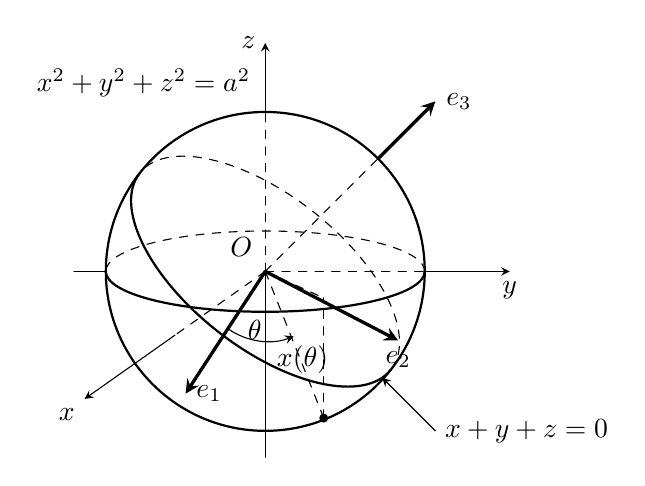
\begin{tikzpicture}[scale=1.35, >=stealth, line cap=round, line join=round]
    % 球面外轮廓圆
    \draw[thick] (0,0) circle (1.5);
    
    % 赤道椭圆: 前半实线，后半虚线
    \draw[dashed] (1.5,0) arc (0:180:1.5 and 0.38);
    \draw[thick] (-1.5,0) arc (180:360:1.5 and 0.38);
    
    % 坐标轴: 原点 O 在球心
    % z 轴向上
    \draw[dashed] (0,0) -- (0,1.5);
    \draw[->] (0,1.5) -- (0,2.15) node[left] {$z$};
    \draw (0,0) -- (0,-1.75);
    
    % y 轴向右水平
    \draw[dashed] (0,0) -- (1.5,0);
    \draw[->] (1.5,0) -- (2.3,0) node[below] {$y$};
    \draw (-1.8,0) -- (-1.5,0);
    
    % x 轴向左前斜下方 (约 215 度)
    \draw[dashed] (0,0) -- (-0.85,-0.6);
    \draw[->] (-0.85,-0.6) -- (-1.7,-1.2) node[below left] {$x$};
    
    % 原点标签 O
    \node[above left] at (-0.03,0.05) {$O$};
    
    % 平面 x+y+z=0 截球的大圆椭圆 C:
    % 原书显示为一个倾斜的大椭圆，长轴约沿 -40°/140° 方向，前半实线，后半虚线
    \begin{scope}[rotate=-38]
      \draw[thick] (-1.5,0) arc (180:360:1.5 and 0.72);
      \draw[dashed] (1.5,0) arc (0:180:1.5 and 0.72);
    \end{scope}
    
    % 基底向量 e_3 (法向量 n0 方向，即 (1,1,1) 方向，在图中指向右上方)
    \draw[dashed] (0,0) -- (1.06,1.06);
    \draw[->,very thick] (1.06,1.06) -- (1.6,1.6) node[right] {$\boldsymbol{e}_{3}$};
    
    % 截面平面内正交基底 e_1 与 e_2:
    % e_1 指向左下方
    \draw[->,very thick] (0,0) -- (-0.75,-1.15) node[right] {$\boldsymbol{e}_{1}$};
    
    % e_2 指向右下方
    \draw[->,very thick] (0,0) -- (1.25,-0.65) node[below] {$\boldsymbol{e}_{2}$};
    
    % 在 C 上取点 x(theta):
    \draw[dashed] (0,0) -- (0.55,-1.38);
    \fill (0.55,-1.38) circle (1.2pt);
    \node[above] at (0.35,-1.05) {$\boldsymbol{x}(\theta)$};
    
    % theta 角弧线 (从 e_1 到 x(theta))
    \draw[->] (-0.35,-0.54) arc (-125:-68:0.65);
    \node at (-0.1,-0.55) {$\theta$};
    
    % 竖直投影辅助虚线: 从 x(theta) 向上做垂直辅助线到赤道面
    \draw[dashed] (0.55,-1.38) -- (0.55,-0.25);
    \draw[dashed] (0,0) -- (0.55,-0.25);
    
    % 公式标注:
    % 左上角: x^2 + y^2 + z^2 = a^2
    \node[above left] at (-0.05,1.55) {$x^{2}+y^{2}+z^{2}=a^{2}$};
    % 右下角: x + y + z = 0 指向截面大圆
    \draw[<-] (1.1,-1.0) -- (1.6,-1.5) node[right] {$x+y+z=0$};
  \end{tikzpicture}
  \caption{}\label{fig:11.1.1}
\end{figure}

于是, 半径为 $a$ 的圆 $C$ 的弧长元为 $\mathrm{d} s=a\,\mathrm{d} \theta$, 或者
\[
  \mathrm{d} s=\left\|\boldsymbol{x}^{\prime}(\theta)\right\| \mathrm{d} \theta=\left\|a\left(-\sin \theta\, \boldsymbol{e}_{1}+\cos \theta\, \boldsymbol{e}_{2}\right)\right\|=a\,\mathrm{d} \theta.
\]
因此, 第一型曲线积分
\begin{align*}
  \int_{C} x y\,\mathrm{d} s &=\int_{0}^{2 \pi} a\left(\frac{1}{\sqrt{6}} \cos \theta+\frac{1}{\sqrt{2}} \sin \theta\right) \cdot a\left(-\frac{2}{\sqrt{6}} \cos \theta\right) \cdot a\,\mathrm{d} \theta \\
  &=a^{3} \int_{0}^{2 \pi}\left(-\frac{2}{6} \cos ^{2} \theta-\sqrt{\frac{2}{6}} \sin \theta \cos \theta\right) \mathrm{d} \theta \\
  &=-\frac{1}{3} a^{3} \int_{0}^{2 \pi} \cos ^{2} \theta\,\mathrm{d} \theta=-\frac{1}{3} a^{3} \int_{0}^{2 \pi} \frac{1+\cos 2 \theta}{2}\,\mathrm{d} \theta \\
  &=-\frac{1}{3} a^{3}\left(\pi+\frac{1}{2} \sin 2 \theta\bigg|_{0} ^{2 \pi}\right)=-\frac{1}{3} \pi a^{3}. \qedhere
\end{align*}
\end{solution}

\begin{solution}[解法 2 (利用对称性)]
由代数与几何两方面的对称性, 有
\[
  \int_{C} x y\,\mathrm{d} s=\int_{C} y z\,\mathrm{d} s=\int_{C} z x\,\mathrm{d} s,
\]
所以,
\begin{align*}
  \int_{C} x y\,\mathrm{d} s &=\frac{1}{3} \int_{C}(x y+y z+z x)\,\mathrm{d} s \\
  &=\frac{1}{6} \int_{C}\left[(x+y+z)^{2}-\left(x^{2}+y^{2}+z^{2}\right)\right] \mathrm{d} s \\
  &=\frac{1}{6} \int_{C}\left(0^{2}-a^{2}\right) \mathrm{d} s=-\frac{1}{6} a^{2} s(C)=-\frac{1}{6} a^{2} \cdot 2 \pi a=-\frac{1}{3} \pi a^{3}. \qedhere
\end{align*}
\end{solution}

上面讨论的第一型曲线积分与曲线的弧长关系密切. 第一型曲面积分与曲面面积的关联也很密切. 因此, 我们必须从曲面的面积讲起.

许多平面图形的面积计算公式, 早在 Euclid 的\textit{几何原本}出现之前就已经建立起来了. 特别是平面多边形的面积计算, 也许是更早一些的事. 对于一般的平面上有界点集的面积, 在\extref{定义 10.2.2}中已经通过二重积分给出.

多面体的表面是由一些平面多边形组成的, 其表面积就是这些平面多边形的面积之和, 因此多面体的表面积的计算就被认为是解决了. 对于弯曲的曲面, 它的面积, 人们想到用内接于该曲面的若干平面三角形组成的图形 (称为折面) 的表面积来逼近是很自然的事. 曲线的弧长正是用内接于该曲线的连续折线的长度来逼近的. 对于弯曲的曲面抱有类似的希望又有什么不合理的呢? 但是, 19 世纪末, H. A. Schwarz 给出了一个著名的例子说明, 即使对于非常简单的曲面, 这种想法也是行不通的.

考虑一个底半径为 $1$, 高为 $1$ 的直圆柱面 $\Sigma$. 若将 $\Sigma$ 沿一条母线剪开, 然后将它平铺在平面上, 就变成了一个边长为 $1$ 与 $2 \pi$ 的矩形. 这个矩形的面积等于 $2 \pi$, 因此 $\Sigma$ 的表面积就应当等于 $2 \pi$. Schwarz 考虑用折面来逼近这个直圆柱面: 用与母线垂直的, 间隔均匀的 $m+1$ 张平面去分割这个直圆柱面, 截出 $m+1$ 个圆周. 然后在每个这样的圆周上, 用 $n$ 个分点将它等分. 这些分点是这样分布的: 上一个圆周上的分点对最靠近它的下一圆周的垂直投影与下一圆周上的相邻两个分点有相等的距离. \cref{fig:11.1.2}中的分点 $A$ 与 $B$, $C$ 就代表这种关系.

\begin{figure}[htbp]
  \centering
  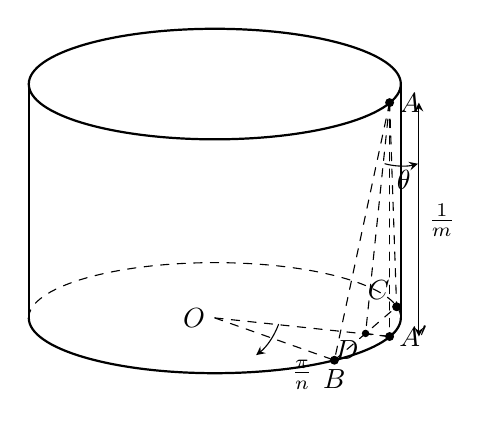
\begin{tikzpicture}[scale=1.35, >=stealth, line cap=round, line join=round]
    % 圆柱顶底面椭圆
    \draw[thick] (0,2.2) ellipse (1.75 and 0.52);
    \draw[dashed] (-1.75,0) arc (180:0:1.75 and 0.52);
    \draw[thick] (-1.75,0) arc (180:360:1.75 and 0.52);
    % 两侧竖直母线
    \draw[thick] (-1.75,2.2) -- (-1.75,0);
    \draw[thick] (1.75,2.2) -- (1.75,0);
    
    % 底面圆心 O
    \coordinate (Obot) at (0,0);
    \node[left] at (Obot) {$O$};
    
    % 顶面点 A
    \coordinate (A) at (1.644, 2.025);
    \fill (A) circle (1.2pt) node[right] {$A$};
    
    % 底面对应投影点 A'
    \coordinate (Ap) at (1.644, -0.175);
    \fill (Ap) circle (1.2pt) node[right] {$A'$};
    \draw[dashed] (A) -- (Ap);
    
    % 高度 1/m
    \draw[<->] (1.92, 2.025) -- (1.92, -0.175);
    \node[right] at (1.92, 0.92) {$\frac{1}{m}$};
    
    % 底面相邻分点 B 和 C
    \coordinate (B) at (1.125, -0.398);
    \coordinate (C) at (1.710, 0.105);
    \fill (B) circle (1.2pt) node[below] {$B$};
    \fill (C) circle (1.2pt) node[above left=-1pt] {$C$};
    
    % 弦 BC 的中点 D
    \coordinate (D) at (1.418, -0.146);
    \fill (D) circle (1.0pt) node[below left=-1pt] {$D$};
    \draw[dashed] (B) -- (C);
    
    % 从 O 连虚线到 A' 和 B
    \draw[dashed] (Obot) -- (Ap);
    \draw[dashed] (Obot) -- (B);
    
    % 夹角 pi/n 在 O 处引出
    \draw[->] (0.60, -0.06) arc (-20:-52:0.65);
    \node[below=1pt] at (0.82, -0.28) {$\frac{\pi}{n}$};
    
    % 连线 A'D
    \draw[dashed] (Ap) -- (D);
    
    % 三角形 ABC 及其在侧面的斜向连线
    \draw[dashed] (A) -- (B);
    \draw[dashed] (A) -- (C);
    \draw[dashed] (A) -- (D);
    
    % 夹角 theta (AA' 与 AD 在 A 点的夹角)
    \draw[->] (1.60, 1.45) arc (-105:-75:0.6);
    \node[right] at (1.62, 1.30) {$\theta$};
  \end{tikzpicture}
  \caption{}\label{fig:11.1.2}
\end{figure}

再将 $A, B, C$ 三点连成一个三角形, 并且设想所有的有这种关系的三个分点都被这样地连成了三角形, 造成了\cref{fig:11.1.3}那样的模型, 它是一个内接于直圆柱面的折面. 这个折面由 $2 m n$ 个全等的三角形组成.

在\cref{fig:11.1.2}中, $\angle B O A^{\prime}=\frac{\pi}{n}$, 从而 $A^{\prime} D=1-\cos \frac{\pi}{n}$, 所以,
\begin{align*}
  A D &=\sqrt{A^{\prime} A^{2}+A^{\prime} D^{2}} \\
      &=\sqrt{\left(\frac{1}{m}\right)^{2}+\left(1-\cos \frac{\pi}{n}\right)^{2}}.
\end{align*}

于是, 三角形 $A B C$ 的面积为
\begin{align*}
  \frac{1}{2} B C \cdot A D &=B D \cdot A D \\
                            &=\sin \frac{\pi}{n} \sqrt{\left(\frac{1}{m}\right)^{2}+\left(1-\cos \frac{\pi}{n}\right)^{2}}.
\end{align*}

\begin{figure}[htbp]
  \centering
  \begin{tikzpicture}[scale=1.1, >=stealth, line cap=round, line join=round]
    \draw[dashed, thin, black!65] (1.516,-1.833) -- (1.690,-1.275);
    \draw[dashed, thin, black!65] (1.750,-1.754) -- (1.690,-1.275);
    \draw[dashed, thin, black!65] (1.750,-1.754) -- (1.237,-1.204);
    \draw[dashed, thin, black!65] (1.516,-1.675) -- (1.237,-1.204);
    \draw[dashed, thin, black!65] (1.516,-1.675) -- (0.453,-1.163);
    \draw[dashed, thin, black!65] (0.875,-1.617) -- (0.453,-1.163);
    \draw[dashed, thin, black!65] (0.875,-1.617) -- (-0.453,-1.163);
    \draw[dashed, thin, black!65] (0.000,-1.596) -- (-0.453,-1.163);
    \draw[dashed, thin, black!65] (0.000,-1.596) -- (-1.237,-1.204);
    \draw[dashed, thin, black!65] (-0.875,-1.617) -- (-1.237,-1.204);
    \draw[dashed, thin, black!65] (-0.875,-1.617) -- (-1.690,-1.275);
    \draw[dashed, thin, black!65] (-1.516,-1.675) -- (-1.690,-1.275);
    \draw[dashed, thin, black!65] (-1.516,-1.675) -- (-1.690,-1.356);
    \draw[dashed, thin, black!65] (1.690,-1.275) -- (1.750,-0.877);
    \draw[dashed, thin, black!65] (1.690,-1.275) -- (1.516,-0.798);
    \draw[dashed, thin, black!65] (1.237,-1.204) -- (1.516,-0.798);
    \draw[dashed, thin, black!65] (1.237,-1.204) -- (0.875,-0.741);
    \draw[dashed, thin, black!65] (0.453,-1.163) -- (0.875,-0.741);
    \draw[dashed, thin, black!65] (0.453,-1.163) -- (0.000,-0.719);
    \draw[dashed, thin, black!65] (-0.453,-1.163) -- (0.000,-0.719);
    \draw[dashed, thin, black!65] (-0.453,-1.163) -- (-0.875,-0.741);
    \draw[dashed, thin, black!65] (-1.237,-1.204) -- (-0.875,-0.741);
    \draw[dashed, thin, black!65] (-1.237,-1.204) -- (-1.516,-0.798);
    \draw[dashed, thin, black!65] (-1.690,-1.275) -- (-1.516,-0.798);
    \draw[dashed, thin, black!65] (-1.690,-1.275) -- (-1.750,-0.877);
    \draw[dashed, thin, black!65] (1.516,-0.956) -- (1.690,-0.398);
    \draw[dashed, thin, black!65] (1.750,-0.877) -- (1.690,-0.398);
    \draw[dashed, thin, black!65] (1.750,-0.877) -- (1.237,-0.327);
    \draw[dashed, thin, black!65] (1.516,-0.798) -- (1.237,-0.327);
    \draw[dashed, thin, black!65] (1.516,-0.798) -- (0.453,-0.286);
    \draw[dashed, thin, black!65] (0.875,-0.741) -- (0.453,-0.286);
    \draw[dashed, thin, black!65] (0.875,-0.741) -- (-0.453,-0.286);
    \draw[dashed, thin, black!65] (0.000,-0.719) -- (-0.453,-0.286);
    \draw[dashed, thin, black!65] (0.000,-0.719) -- (-1.237,-0.327);
    \draw[dashed, thin, black!65] (-0.875,-0.741) -- (-1.237,-0.327);
    \draw[dashed, thin, black!65] (-0.875,-0.741) -- (-1.690,-0.398);
    \draw[dashed, thin, black!65] (-1.516,-0.798) -- (-1.690,-0.398);
    \draw[dashed, thin, black!65] (-1.516,-0.798) -- (-1.690,-0.479);
    \draw[dashed, thin, black!65] (1.690,-0.398) -- (1.750,0.000);
    \draw[dashed, thin, black!65] (1.690,-0.398) -- (1.516,0.079);
    \draw[dashed, thin, black!65] (1.237,-0.327) -- (1.516,0.079);
    \draw[dashed, thin, black!65] (1.237,-0.327) -- (0.875,0.136);
    \draw[dashed, thin, black!65] (0.453,-0.286) -- (0.875,0.136);
    \draw[dashed, thin, black!65] (0.453,-0.286) -- (0.000,0.157);
    \draw[dashed, thin, black!65] (-0.453,-0.286) -- (0.000,0.157);
    \draw[dashed, thin, black!65] (-0.453,-0.286) -- (-0.875,0.136);
    \draw[dashed, thin, black!65] (-1.237,-0.327) -- (-0.875,0.136);
    \draw[dashed, thin, black!65] (-1.237,-0.327) -- (-1.516,0.079);
    \draw[dashed, thin, black!65] (-1.690,-0.398) -- (-1.516,0.079);
    \draw[dashed, thin, black!65] (-1.690,-0.398) -- (-1.750,0.000);
    \draw[dashed, thin, black!65] (1.516,-0.079) -- (1.690,0.479);
    \draw[dashed, thin, black!65] (1.750,0.000) -- (1.690,0.479);
    \draw[dashed, thin, black!65] (1.750,0.000) -- (1.237,0.550);
    \draw[dashed, thin, black!65] (1.516,0.079) -- (1.237,0.550);
    \draw[dashed, thin, black!65] (1.516,0.079) -- (0.453,0.591);
    \draw[dashed, thin, black!65] (0.875,0.136) -- (0.453,0.591);
    \draw[dashed, thin, black!65] (0.875,0.136) -- (-0.453,0.591);
    \draw[dashed, thin, black!65] (0.000,0.157) -- (-0.453,0.591);
    \draw[dashed, thin, black!65] (0.000,0.157) -- (-1.237,0.550);
    \draw[dashed, thin, black!65] (-0.875,0.136) -- (-1.237,0.550);
    \draw[dashed, thin, black!65] (-0.875,0.136) -- (-1.690,0.479);
    \draw[dashed, thin, black!65] (-1.516,0.079) -- (-1.690,0.479);
    \draw[dashed, thin, black!65] (-1.516,0.079) -- (-1.690,0.398);
    \draw[dashed, thin, black!65] (1.690,0.479) -- (1.750,0.877);
    \draw[dashed, thin, black!65] (1.690,0.479) -- (1.516,0.956);
    \draw[dashed, thin, black!65] (1.237,0.550) -- (1.516,0.956);
    \draw[dashed, thin, black!65] (1.237,0.550) -- (0.875,1.013);
    \draw[dashed, thin, black!65] (0.453,0.591) -- (0.875,1.013);
    \draw[dashed, thin, black!65] (0.453,0.591) -- (0.000,1.034);
    \draw[dashed, thin, black!65] (-0.453,0.591) -- (0.000,1.034);
    \draw[dashed, thin, black!65] (-0.453,0.591) -- (-0.875,1.013);
    \draw[dashed, thin, black!65] (-1.237,0.550) -- (-0.875,1.013);
    \draw[dashed, thin, black!65] (-1.237,0.550) -- (-1.516,0.956);
    \draw[dashed, thin, black!65] (-1.690,0.479) -- (-1.516,0.956);
    \draw[dashed, thin, black!65] (-1.690,0.479) -- (-1.750,0.877);
    \draw[dashed, thin, black!65] (1.516,0.798) -- (1.690,1.356);
    \draw[dashed, thin, black!65] (1.750,0.877) -- (1.690,1.356);
    \draw[dashed, thin, black!65] (1.750,0.877) -- (1.237,1.427);
    \draw[dashed, thin, black!65] (1.516,0.956) -- (1.237,1.427);
    \draw[dashed, thin, black!65] (1.516,0.956) -- (0.453,1.467);
    \draw[dashed, thin, black!65] (0.875,1.013) -- (0.453,1.467);
    \draw[dashed, thin, black!65] (0.875,1.013) -- (-0.453,1.467);
    \draw[dashed, thin, black!65] (0.000,1.034) -- (-0.453,1.467);
    \draw[dashed, thin, black!65] (0.000,1.034) -- (-1.237,1.427);
    \draw[dashed, thin, black!65] (-0.875,1.013) -- (-1.237,1.427);
    \draw[dashed, thin, black!65] (-0.875,1.013) -- (-1.690,1.356);
    \draw[dashed, thin, black!65] (-1.516,0.956) -- (-1.690,1.356);
    \draw[dashed, thin, black!65] (-1.516,0.956) -- (-1.690,1.275);
    \draw[dashed, thin, black!65] (1.690,1.356) -- (1.750,1.754);
    \draw[dashed, thin, black!65] (1.690,1.356) -- (1.516,1.833);
    \draw[dashed, thin, black!65] (1.237,1.427) -- (1.516,1.833);
    \draw[dashed, thin, black!65] (1.237,1.427) -- (0.875,1.890);
    \draw[dashed, thin, black!65] (0.453,1.467) -- (0.875,1.890);
    \draw[dashed, thin, black!65] (0.453,1.467) -- (0.000,1.911);
    \draw[dashed, thin, black!65] (-0.453,1.467) -- (0.000,1.911);
    \draw[dashed, thin, black!65] (-0.453,1.467) -- (-0.875,1.890);
    \draw[dashed, thin, black!65] (-1.237,1.427) -- (-0.875,1.890);
    \draw[dashed, thin, black!65] (-1.237,1.427) -- (-1.516,1.833);
    \draw[dashed, thin, black!65] (-1.690,1.356) -- (-1.516,1.833);
    \draw[dashed, thin, black!65] (-1.690,1.356) -- (-1.750,1.754);
    \draw[dashed, thin, black!65] (1.750,-1.754) -- (1.516,-1.675);
    \draw[dashed, thin, black!65] (1.516,-1.675) -- (0.875,-1.617);
    \draw[dashed, thin, black!65] (0.875,-1.617) -- (0.000,-1.596);
    \draw[dashed, thin, black!65] (0.000,-1.596) -- (-0.875,-1.617);
    \draw[dashed, thin, black!65] (-0.875,-1.617) -- (-1.516,-1.675);
    \draw[dashed, thin, black!65] (-1.516,-1.675) -- (-1.750,-1.754);
    \draw[dashed, thin, black!65] (1.690,-1.356) -- (1.690,-1.275);
    \draw[dashed, thin, black!65] (1.690,-1.275) -- (1.237,-1.204);
    \draw[dashed, thin, black!65] (1.237,-1.204) -- (0.453,-1.163);
    \draw[dashed, thin, black!65] (0.453,-1.163) -- (-0.453,-1.163);
    \draw[dashed, thin, black!65] (-0.453,-1.163) -- (-1.237,-1.204);
    \draw[dashed, thin, black!65] (-1.237,-1.204) -- (-1.690,-1.275);
    \draw[dashed, thin, black!65] (-1.690,-1.275) -- (-1.690,-1.356);
    \draw[dashed, thin, black!65] (1.750,-0.877) -- (1.516,-0.798);
    \draw[dashed, thin, black!65] (1.516,-0.798) -- (0.875,-0.741);
    \draw[dashed, thin, black!65] (0.875,-0.741) -- (0.000,-0.719);
    \draw[dashed, thin, black!65] (0.000,-0.719) -- (-0.875,-0.741);
    \draw[dashed, thin, black!65] (-0.875,-0.741) -- (-1.516,-0.798);
    \draw[dashed, thin, black!65] (-1.516,-0.798) -- (-1.750,-0.877);
    \draw[dashed, thin, black!65] (1.690,-0.479) -- (1.690,-0.398);
    \draw[dashed, thin, black!65] (1.690,-0.398) -- (1.237,-0.327);
    \draw[dashed, thin, black!65] (1.237,-0.327) -- (0.453,-0.286);
    \draw[dashed, thin, black!65] (0.453,-0.286) -- (-0.453,-0.286);
    \draw[dashed, thin, black!65] (-0.453,-0.286) -- (-1.237,-0.327);
    \draw[dashed, thin, black!65] (-1.237,-0.327) -- (-1.690,-0.398);
    \draw[dashed, thin, black!65] (-1.690,-0.398) -- (-1.690,-0.479);
    \draw[dashed, thin, black!65] (1.750,0.000) -- (1.516,0.079);
    \draw[dashed, thin, black!65] (1.516,0.079) -- (0.875,0.136);
    \draw[dashed, thin, black!65] (0.875,0.136) -- (0.000,0.157);
    \draw[dashed, thin, black!65] (0.000,0.157) -- (-0.875,0.136);
    \draw[dashed, thin, black!65] (-0.875,0.136) -- (-1.516,0.079);
    \draw[dashed, thin, black!65] (-1.516,0.079) -- (-1.750,0.000);
    \draw[dashed, thin, black!65] (1.690,0.398) -- (1.690,0.479);
    \draw[dashed, thin, black!65] (1.690,0.479) -- (1.237,0.550);
    \draw[dashed, thin, black!65] (1.237,0.550) -- (0.453,0.591);
    \draw[dashed, thin, black!65] (0.453,0.591) -- (-0.453,0.591);
    \draw[dashed, thin, black!65] (-0.453,0.591) -- (-1.237,0.550);
    \draw[dashed, thin, black!65] (-1.237,0.550) -- (-1.690,0.479);
    \draw[dashed, thin, black!65] (-1.690,0.479) -- (-1.690,0.398);
    \draw[dashed, thin, black!65] (1.750,0.877) -- (1.516,0.956);
    \draw[dashed, thin, black!65] (1.516,0.956) -- (0.875,1.013);
    \draw[dashed, thin, black!65] (0.875,1.013) -- (0.000,1.034);
    \draw[dashed, thin, black!65] (0.000,1.034) -- (-0.875,1.013);
    \draw[dashed, thin, black!65] (-0.875,1.013) -- (-1.516,0.956);
    \draw[dashed, thin, black!65] (-1.516,0.956) -- (-1.750,0.877);
    \draw[dashed, thin, black!65] (1.690,1.275) -- (1.690,1.356);
    \draw[dashed, thin, black!65] (1.690,1.356) -- (1.237,1.427);
    \draw[dashed, thin, black!65] (1.237,1.427) -- (0.453,1.467);
    \draw[dashed, thin, black!65] (0.453,1.467) -- (-0.453,1.467);
    \draw[dashed, thin, black!65] (-0.453,1.467) -- (-1.237,1.427);
    \draw[dashed, thin, black!65] (-1.237,1.427) -- (-1.690,1.356);
    \draw[dashed, thin, black!65] (-1.690,1.356) -- (-1.690,1.275);
    \draw[dashed, thin, black!65] (1.750,1.754) -- (1.516,1.833);
    \draw[dashed, thin, black!65] (1.516,1.833) -- (0.875,1.890);
    \draw[dashed, thin, black!65] (0.875,1.890) -- (0.000,1.911);
    \draw[dashed, thin, black!65] (0.000,1.911) -- (-0.875,1.890);
    \draw[dashed, thin, black!65] (-0.875,1.890) -- (-1.516,1.833);
    \draw[dashed, thin, black!65] (-1.516,1.833) -- (-1.750,1.754);
    \draw[thick] (0.000,-1.911) -- (0.453,-1.467);
    \draw[thick] (0.000,-1.911) -- (1.237,-1.427);
    \draw[thick] (0.875,-1.890) -- (1.237,-1.427);
    \draw[thick] (0.875,-1.890) -- (1.690,-1.356);
    \draw[thick] (1.516,-1.833) -- (1.690,-1.356);
    \draw[thick] (1.516,-1.833) -- (1.690,-1.275);
    \draw[thick] (1.750,-1.754) -- (1.690,-1.275);
    \draw[thick] (1.750,-1.754) -- (1.237,-1.204);
    \draw[thick] (-1.516,-1.675) -- (-1.690,-1.356);
    \draw[thick] (-1.750,-1.754) -- (-1.690,-1.356);
    \draw[thick] (-1.750,-1.754) -- (-1.237,-1.427);
    \draw[thick] (-1.516,-1.833) -- (-1.237,-1.427);
    \draw[thick] (-1.516,-1.833) -- (-0.453,-1.467);
    \draw[thick] (-0.875,-1.890) -- (-0.453,-1.467);
    \draw[thick] (-0.875,-1.890) -- (0.453,-1.467);
    \draw[thick] (0.453,-1.467) -- (0.000,-1.034);
    \draw[thick] (0.453,-1.467) -- (0.875,-1.013);
    \draw[thick] (1.237,-1.427) -- (0.875,-1.013);
    \draw[thick] (1.237,-1.427) -- (1.516,-0.956);
    \draw[thick] (1.690,-1.356) -- (1.516,-0.956);
    \draw[thick] (1.690,-1.356) -- (1.750,-0.877);
    \draw[thick] (1.690,-1.275) -- (1.750,-0.877);
    \draw[thick] (-1.690,-1.275) -- (-1.750,-0.877);
    \draw[thick] (-1.690,-1.356) -- (-1.750,-0.877);
    \draw[thick] (-1.690,-1.356) -- (-1.516,-0.956);
    \draw[thick] (-1.237,-1.427) -- (-1.516,-0.956);
    \draw[thick] (-1.237,-1.427) -- (-0.875,-1.013);
    \draw[thick] (-0.453,-1.467) -- (-0.875,-1.013);
    \draw[thick] (-0.453,-1.467) -- (0.000,-1.034);
    \draw[thick] (0.000,-1.034) -- (0.453,-0.591);
    \draw[thick] (0.000,-1.034) -- (1.237,-0.550);
    \draw[thick] (0.875,-1.013) -- (1.237,-0.550);
    \draw[thick] (0.875,-1.013) -- (1.690,-0.479);
    \draw[thick] (1.516,-0.956) -- (1.690,-0.479);
    \draw[thick] (1.516,-0.956) -- (1.690,-0.398);
    \draw[thick] (1.750,-0.877) -- (1.690,-0.398);
    \draw[thick] (1.750,-0.877) -- (1.237,-0.327);
    \draw[thick] (-1.516,-0.798) -- (-1.690,-0.479);
    \draw[thick] (-1.750,-0.877) -- (-1.690,-0.479);
    \draw[thick] (-1.750,-0.877) -- (-1.237,-0.550);
    \draw[thick] (-1.516,-0.956) -- (-1.237,-0.550);
    \draw[thick] (-1.516,-0.956) -- (-0.453,-0.591);
    \draw[thick] (-0.875,-1.013) -- (-0.453,-0.591);
    \draw[thick] (-0.875,-1.013) -- (0.453,-0.591);
    \draw[thick] (0.453,-0.591) -- (0.000,-0.157);
    \draw[thick] (0.453,-0.591) -- (0.875,-0.136);
    \draw[thick] (1.237,-0.550) -- (0.875,-0.136);
    \draw[thick] (1.237,-0.550) -- (1.516,-0.079);
    \draw[thick] (1.690,-0.479) -- (1.516,-0.079);
    \draw[thick] (1.690,-0.479) -- (1.750,0.000);
    \draw[thick] (1.690,-0.398) -- (1.750,0.000);
    \draw[thick] (-1.690,-0.398) -- (-1.750,0.000);
    \draw[thick] (-1.690,-0.479) -- (-1.750,0.000);
    \draw[thick] (-1.690,-0.479) -- (-1.516,-0.079);
    \draw[thick] (-1.237,-0.550) -- (-1.516,-0.079);
    \draw[thick] (-1.237,-0.550) -- (-0.875,-0.136);
    \draw[thick] (-0.453,-0.591) -- (-0.875,-0.136);
    \draw[thick] (-0.453,-0.591) -- (0.000,-0.157);
    \draw[thick] (0.000,-0.157) -- (0.453,0.286);
    \draw[thick] (0.000,-0.157) -- (1.237,0.327);
    \draw[thick] (0.875,-0.136) -- (1.237,0.327);
    \draw[thick] (0.875,-0.136) -- (1.690,0.398);
    \draw[thick] (1.516,-0.079) -- (1.690,0.398);
    \draw[thick] (1.516,-0.079) -- (1.690,0.479);
    \draw[thick] (1.750,0.000) -- (1.690,0.479);
    \draw[thick] (1.750,0.000) -- (1.237,0.550);
    \draw[thick] (-1.516,0.079) -- (-1.690,0.398);
    \draw[thick] (-1.750,0.000) -- (-1.690,0.398);
    \draw[thick] (-1.750,0.000) -- (-1.237,0.327);
    \draw[thick] (-1.516,-0.079) -- (-1.237,0.327);
    \draw[thick] (-1.516,-0.079) -- (-0.453,0.286);
    \draw[thick] (-0.875,-0.136) -- (-0.453,0.286);
    \draw[thick] (-0.875,-0.136) -- (0.453,0.286);
    \draw[thick] (0.453,0.286) -- (0.000,0.719);
    \draw[thick] (0.453,0.286) -- (0.875,0.741);
    \draw[thick] (1.237,0.327) -- (0.875,0.741);
    \draw[thick] (1.237,0.327) -- (1.516,0.798);
    \draw[thick] (1.690,0.398) -- (1.516,0.798);
    \draw[thick] (1.690,0.398) -- (1.750,0.877);
    \draw[thick] (1.690,0.479) -- (1.750,0.877);
    \draw[thick] (-1.690,0.479) -- (-1.750,0.877);
    \draw[thick] (-1.690,0.398) -- (-1.750,0.877);
    \draw[thick] (-1.690,0.398) -- (-1.516,0.798);
    \draw[thick] (-1.237,0.327) -- (-1.516,0.798);
    \draw[thick] (-1.237,0.327) -- (-0.875,0.741);
    \draw[thick] (-0.453,0.286) -- (-0.875,0.741);
    \draw[thick] (-0.453,0.286) -- (0.000,0.719);
    \draw[thick] (0.000,0.719) -- (0.453,1.163);
    \draw[thick] (0.000,0.719) -- (1.237,1.204);
    \draw[thick] (0.875,0.741) -- (1.237,1.204);
    \draw[thick] (0.875,0.741) -- (1.690,1.275);
    \draw[thick] (1.516,0.798) -- (1.690,1.275);
    \draw[thick] (1.516,0.798) -- (1.690,1.356);
    \draw[thick] (1.750,0.877) -- (1.690,1.356);
    \draw[thick] (1.750,0.877) -- (1.237,1.427);
    \draw[thick] (-1.516,0.956) -- (-1.690,1.275);
    \draw[thick] (-1.750,0.877) -- (-1.690,1.275);
    \draw[thick] (-1.750,0.877) -- (-1.237,1.204);
    \draw[thick] (-1.516,0.798) -- (-1.237,1.204);
    \draw[thick] (-1.516,0.798) -- (-0.453,1.163);
    \draw[thick] (-0.875,0.741) -- (-0.453,1.163);
    \draw[thick] (-0.875,0.741) -- (0.453,1.163);
    \draw[thick] (0.453,1.163) -- (0.000,1.596);
    \draw[thick] (0.453,1.163) -- (0.875,1.617);
    \draw[thick] (1.237,1.204) -- (0.875,1.617);
    \draw[thick] (1.237,1.204) -- (1.516,1.675);
    \draw[thick] (1.690,1.275) -- (1.516,1.675);
    \draw[thick] (1.690,1.275) -- (1.750,1.754);
    \draw[thick] (1.690,1.356) -- (1.750,1.754);
    \draw[thick] (-1.690,1.356) -- (-1.750,1.754);
    \draw[thick] (-1.690,1.275) -- (-1.750,1.754);
    \draw[thick] (-1.690,1.275) -- (-1.516,1.675);
    \draw[thick] (-1.237,1.204) -- (-1.516,1.675);
    \draw[thick] (-1.237,1.204) -- (-0.875,1.617);
    \draw[thick] (-0.453,1.163) -- (-0.875,1.617);
    \draw[thick] (-0.453,1.163) -- (0.000,1.596);
    \draw[thick] (0.000,-1.911) -- (0.875,-1.890);
    \draw[thick] (0.875,-1.890) -- (1.516,-1.833);
    \draw[thick] (1.516,-1.833) -- (1.750,-1.754);
    \draw[thick] (1.750,-1.754) -- (1.516,-1.675);
    \draw[thick] (-1.516,-1.675) -- (-1.750,-1.754);
    \draw[thick] (-1.750,-1.754) -- (-1.516,-1.833);
    \draw[thick] (-1.516,-1.833) -- (-0.875,-1.890);
    \draw[thick] (-0.875,-1.890) -- (0.000,-1.911);
    \draw[thick] (0.453,-1.467) -- (1.237,-1.427);
    \draw[thick] (1.237,-1.427) -- (1.690,-1.356);
    \draw[thick] (1.690,-1.356) -- (1.690,-1.275);
    \draw[thick] (-1.690,-1.275) -- (-1.690,-1.356);
    \draw[thick] (-1.690,-1.356) -- (-1.237,-1.427);
    \draw[thick] (-1.237,-1.427) -- (-0.453,-1.467);
    \draw[thick] (-0.453,-1.467) -- (0.453,-1.467);
    \draw[thick] (0.000,-1.034) -- (0.875,-1.013);
    \draw[thick] (0.875,-1.013) -- (1.516,-0.956);
    \draw[thick] (1.516,-0.956) -- (1.750,-0.877);
    \draw[thick] (1.750,-0.877) -- (1.516,-0.798);
    \draw[thick] (-1.516,-0.798) -- (-1.750,-0.877);
    \draw[thick] (-1.750,-0.877) -- (-1.516,-0.956);
    \draw[thick] (-1.516,-0.956) -- (-0.875,-1.013);
    \draw[thick] (-0.875,-1.013) -- (0.000,-1.034);
    \draw[thick] (0.453,-0.591) -- (1.237,-0.550);
    \draw[thick] (1.237,-0.550) -- (1.690,-0.479);
    \draw[thick] (1.690,-0.479) -- (1.690,-0.398);
    \draw[thick] (-1.690,-0.398) -- (-1.690,-0.479);
    \draw[thick] (-1.690,-0.479) -- (-1.237,-0.550);
    \draw[thick] (-1.237,-0.550) -- (-0.453,-0.591);
    \draw[thick] (-0.453,-0.591) -- (0.453,-0.591);
    \draw[thick] (0.000,-0.157) -- (0.875,-0.136);
    \draw[thick] (0.875,-0.136) -- (1.516,-0.079);
    \draw[thick] (1.516,-0.079) -- (1.750,0.000);
    \draw[thick] (1.750,0.000) -- (1.516,0.079);
    \draw[thick] (-1.516,0.079) -- (-1.750,0.000);
    \draw[thick] (-1.750,0.000) -- (-1.516,-0.079);
    \draw[thick] (-1.516,-0.079) -- (-0.875,-0.136);
    \draw[thick] (-0.875,-0.136) -- (0.000,-0.157);
    \draw[thick] (0.453,0.286) -- (1.237,0.327);
    \draw[thick] (1.237,0.327) -- (1.690,0.398);
    \draw[thick] (1.690,0.398) -- (1.690,0.479);
    \draw[thick] (-1.690,0.479) -- (-1.690,0.398);
    \draw[thick] (-1.690,0.398) -- (-1.237,0.327);
    \draw[thick] (-1.237,0.327) -- (-0.453,0.286);
    \draw[thick] (-0.453,0.286) -- (0.453,0.286);
    \draw[thick] (0.000,0.719) -- (0.875,0.741);
    \draw[thick] (0.875,0.741) -- (1.516,0.798);
    \draw[thick] (1.516,0.798) -- (1.750,0.877);
    \draw[thick] (1.750,0.877) -- (1.516,0.956);
    \draw[thick] (-1.516,0.956) -- (-1.750,0.877);
    \draw[thick] (-1.750,0.877) -- (-1.516,0.798);
    \draw[thick] (-1.516,0.798) -- (-0.875,0.741);
    \draw[thick] (-0.875,0.741) -- (0.000,0.719);
    \draw[thick] (0.453,1.163) -- (1.237,1.204);
    \draw[thick] (1.237,1.204) -- (1.690,1.275);
    \draw[thick] (1.690,1.275) -- (1.690,1.356);
    \draw[thick] (-1.690,1.356) -- (-1.690,1.275);
    \draw[thick] (-1.690,1.275) -- (-1.237,1.204);
    \draw[thick] (-1.237,1.204) -- (-0.453,1.163);
    \draw[thick] (-0.453,1.163) -- (0.453,1.163);
    \draw[thick] (0.000,1.596) -- (0.875,1.617);
    \draw[thick] (0.875,1.617) -- (1.516,1.675);
    \draw[thick] (1.516,1.675) -- (1.750,1.754);
    \draw[thick] (1.750,1.754) -- (1.516,1.833);
    \draw[thick] (-1.516,1.833) -- (-1.750,1.754);
    \draw[thick] (-1.750,1.754) -- (-1.516,1.675);
    \draw[thick] (-1.516,1.675) -- (-0.875,1.617);
    \draw[thick] (-0.875,1.617) -- (0.000,1.596);
    \node[below=6pt] at (0,-2.3) {折面 由 $2mn$ 个全等三角形组成};
  \end{tikzpicture}
  \caption{}\label{fig:11.1.3}
\end{figure}

因而折面的面积
\begin{align*}
  S_{m, n} &=2 m n \sin \frac{\pi}{n} \sqrt{\left(\frac{1}{m}\right)^{2}+\left(1-\cos \frac{\pi}{n}\right)^{2}} \\
           &=2 n \sin \frac{\pi}{n} \sqrt{1+m^{2}\left(1-\cos \frac{\pi}{n}\right)^{2}}.
\end{align*}

当 $m$ 与 $n$ 同时无限增加时, 所有那些小三角形的直径趋于零, 但 $S_{m, n}$ 无极限. 实际上, 若令 $m$ 与 $n$ 增长时, 使得比值 $\frac{m}{n^{2}}$ 趋向于一个确定的数 $q$, 即
\[
  \lim \frac{m}{n^{2}}=q.
\]
这就立即推得
\begin{align*}
  \lim S_{m, n} &=\lim 2 \pi \frac{\sin \frac{\pi}{n}}{\frac{\pi}{n}} \sqrt{1+\left(\frac{m}{n^{2}}\right)^{2}\left(\frac{1-\cos \frac{\pi}{n}}{\frac{\pi^{2}}{2 n^{2}}}\right)^{2} \frac{\pi^{4}}{4}} \\
                &=2 \pi \sqrt{1+\frac{q^{2}}{4} \pi^{4}}.
\end{align*}

由此可见, 这个极限依赖于比值 $q$ 的大小, 即依赖于 $m$ 与 $n$ 同时增加的方式. 当 $q=0$ 时, 也只在这个时候, 所说的极限等于 $2 \pi$, 这正是中学立体几何教程中给出的面积.

深入地考察一下\cref{fig:11.1.2}, 便能发现毛病之所在. 当 $q=0$ 时, $m$ 与 $n$ 虽然同时趋于无穷大, 但是 $m$ 趋于无穷大的速度远比 $n^{2}$ 趋于无穷大的速度要慢. 因为
\[
  \tan \theta=\frac{A^{\prime} D}{A A^{\prime}}=\frac{1-\cos \frac{\pi}{n}}{\frac{1}{m}}=\frac{1-\cos \frac{\pi}{n}}{\frac{\pi^{2}}{2 n^{2}}} \cdot \frac{m}{n^{2}} \cdot \frac{\pi^{2}}{2} \to \frac{\pi^{2}}{2} q=0 \quad(m, n \to+\infty),
\]
故那些小三角形可以任意地贴近直圆柱面, 这时 $S_{m, n}$ 的极限确能表示直圆柱面的表面积; 当 $q=+\infty$ 时, $\tan \theta \to \frac{\pi^{2}}{2} q=+\infty \ (m, n \to+\infty)$. 正好相反, 此时这些小三角形几乎变得与直圆柱面的母线 (即轴线) 垂直, 也就是说几乎与直圆柱面的切平面垂直.

因此, 只能放弃用内接于曲面的折面的面积的极限来定义该曲面的面积的想法. 在此, 我们也不去讨论最一般的曲面的面积的定义, 而是假定曲面已经有了连续偏导数的参数表示.

用 $u$ 曲线与 $v$ 曲线将曲面 $\Sigma$ 分成小块. 每小块在曲面的切平面上的投影的面积\allowbreak (\cref{fig:11.1.4}) 可以近似地表示为
\[
  \left\|\boldsymbol{x}_{u}^{\prime} \Delta u \times \boldsymbol{x}_{v}^{\prime} \Delta v\right\|=\left\|\boldsymbol{x}_{u}^{\prime} \times \boldsymbol{x}_{v}^{\prime}\right\| \Delta u \Delta v.
\]

这样, 和式
\[
  \sum\left\|\boldsymbol{x}_{u}^{\prime} \times \boldsymbol{x}_{v}^{\prime}\right\| \Delta u \Delta v
\]
就可以当作 $\Sigma$ 的面积的近似值. 加密 $u$ 曲线与 $v$ 曲线, 通过极限过程, 得到曲面 $\Sigma$ 的面积的精确值. 曲面面积的确切定义如下.

\begin{figure}[htbp]
  \centering
  \begin{tikzpicture}[scale=1.1, >=stealth, line cap=round, line join=round]
    % === 左侧: 参数区域 Delta 平面 (u, v) ===
    \begin{scope}[shift={(0,0)}]
      % 坐标轴 u, v
      \draw[->, thick] (0,0) -- (4.2,0) node[below] {$u$};
      \draw[->, thick] (0,0) -- (0,3.2) node[left] {$v$};
      \node[below left] at (0,0) {$O$};
      
      % 参数区域 Delta 的外边界 (一个倾斜椭圆)
      \draw[thick] (2.0,1.8) ellipse (1.7 and 1.15);
      
      % 网格线
      % 竖直网格线
      \draw (1.5,0) -- (1.5,2.9);
      \draw (2.1,0) -- (2.1,3.0);
      % 水平网格线
      \draw (0,1.2) -- (4.3,1.2);
      \draw (0,1.8) -- (4.1,1.8);
      
      % 阴影微元区域 Delta_ij: [u, u+Delta u] x [v, v+Delta v]
      \fill[pattern=crosshatch dots, pattern color=black!70, black!25] (1.5,1.2) rectangle (2.1,1.8);
      \draw[thick] (1.5,1.2) rectangle (2.1,1.8);
      
      % 四个顶点的标签
      \node[below left] at (1.5,1.2) {\scriptsize $(u,v)$};
      \node[below right] at (2.05,1.2) {\scriptsize $(u+\!\Delta u, v)$};
      \node[above left] at (1.5,1.8) {\scriptsize $(u, v+\!\Delta v)$};
      \node[above right] at (2.05,1.8) {\scriptsize $(u+\!\Delta u, v+\!\Delta v)$};
    \end{scope}

    % 映射箭头 x
    \draw[->, very thick] (4.5,1.7) -- (5.4,1.7) node[above, midway] {$\boldsymbol{x}$};

    % === 右侧: 三维空间中的曲面 Sigma ===
    \begin{scope}[shift={(6.0,-0.2)}]
      % 3D 坐标系 (置于曲面下方)
      \begin{scope}[shift={(0.8,0.3)}]
        \draw[->, thick] (0,0) -- (0,1.2) node[left] {$z$};
        \draw[->, thick] (0,0) -- (1.0,0) node[below] {$y$};
        \draw[->, thick] (0,0) -- (-0.55,-0.55) node[below left] {$x$};
        \node[below right] at (0,0) {$O$};
      \end{scope}
      
      % 曲面轮廓 (双曲/马鞍状曲面网格)
      % 四条外边界曲线
      \draw[thick] (0.2,1.2) .. controls (1.5,2.6) and (3.2,3.3) .. (4.3,3.0);
      \draw[thick] (0.2,1.2) .. controls (1.8,0.8) and (2.2,-0.8) .. (2.6,-1.0);
      \draw[thick] (2.6,-1.0) .. controls (3.4,-0.2) and (4.0,1.5) .. (4.9,1.7);
      \draw[thick] (4.3,3.0) .. controls (4.6,2.6) and (4.8,2.1) .. (4.9,1.7);
      
      % 内部的 u 曲线和 v 曲线
      % v 曲线 (纵向)
      \draw[thick] (1.6,0.3) .. controls (2.0,1.4) and (2.1,2.8) .. (1.8,3.4);
      \draw[thick] (2.5,-0.4) .. controls (2.8,1.2) and (3.0,2.6) .. (3.1,3.2);
      
      % u 曲线 (横向)
      \draw[thick] (0.7,1.7) .. controls (2.0,1.2) and (3.2,2.0) .. (4.5,2.3);
      \draw[thick] (1.2,1.2) .. controls (2.2,0.7) and (3.0,1.4) .. (4.4,1.8);
      
      % 曲面上的微元曲面块 (阴影填充)
      % 顶点对应: P(u,v), P_u, P_v, P_uv
      \coordinate (P00) at (2.05, 0.95);
      \coordinate (P10) at (2.80, 1.15);
      \coordinate (P01) at (1.95, 1.62);
      \coordinate (P11) at (2.75, 1.80);
      
      \fill[pattern=crosshatch dots, pattern color=black!70, black!30] 
        (P00) to[bend left=4] (P10) to[bend right=6] (P11) to[bend right=5] (P01) to[bend left=6] cycle;
        
      % 切平面内的平行四边形微元 (实线线框突出)
      \draw[very thick] (P00) -- (P10) -- (P11) -- (P01) -- cycle;
      
      % 顶点标签
      \node[below=2pt] at (P00) {\scriptsize $\boldsymbol{x}(u,v)$};
      \node[right=2pt] at (P10) {\scriptsize $\boldsymbol{x}(u+\!\Delta u, v)$};
      \node[above left=-1pt] at (P01) {\scriptsize $\boldsymbol{x}(u, v+\!\Delta v)$};
      \node[above right=-1pt] at (P11) {\scriptsize $\boldsymbol{x}(u+\!\Delta u, v+\!\Delta v)$};
    \end{scope}
  \end{tikzpicture}
  \caption{}\label{fig:11.1.4}
\end{figure}

\begin{definition}\label{def:11.1.2}
设 $\Delta$ 为 $\mathbb{R}^{2}$ 中的一个区域, 曲面 $\Sigma$ 有参数表示 $\boldsymbol{x}=\boldsymbol{x}(u, v)=(x(u, v),\allowbreak y(u, v),\allowbreak z(u, v))$, $(u, v) \in \Delta$, 并且设 $\Delta$ 与曲面 $\Sigma$ 上的点有一一对应关系, $\boldsymbol{x}(u, v)$ 是 $C^{1}$ 类的, 在 $\Delta$ 上 $\boldsymbol{x}_{u}^{\prime} \times \boldsymbol{x}_{v}^{\prime} \neq 0$, 即 $\Sigma$ 为正则曲面.

我们称
\[
  \sigma(\Sigma)=\iint_{\Delta}\left\|\boldsymbol{x}_{u}^{\prime} \times \boldsymbol{x}_{v}^{\prime}\right\| \mathrm{d} u \mathrm{d} v
\]
为曲面 $\Sigma$ 的面积, 而称
\[
  \mathrm{d} \boldsymbol{\sigma}=\left\|\boldsymbol{x}_{u}^{\prime} \times \boldsymbol{x}_{v}^{\prime}\right\| \mathrm{d} u \mathrm{d} v
\]
为曲面 $\Sigma$ 的面积元素, 简称面元.
\end{definition}

\begin{lemma}\label{lem:11.1.1}
\cref{def:11.1.2} 不依赖于参数的选择, 即定义是合理的.
\end{lemma}

\begin{proof}
设参数变换 $\boldsymbol{F}: \Delta^{\prime} \to \Delta$, $(s, t) \to (u, v)$ 为 $C^{1}$ 微分同胚, 即 $F$ 为一一映射, $F$ 与 $F^{-1}$ 都是 $C^{1}$ 的. 经变换 $(u, v)=(u(s, t), v(s, t))$ 得到
\begin{align*}
  \left\|\boldsymbol{x}_{s}^{\prime} \times \boldsymbol{x}_{t}^{\prime}\right\| &=\left\|\left(\boldsymbol{x}_{u}^{\prime} u_{s}^{\prime}+\boldsymbol{x}_{v}^{\prime} v_{s}^{\prime}\right) \times\left(\boldsymbol{x}_{u}^{\prime} u_{t}^{\prime}+\boldsymbol{x}_{v}^{\prime} v_{t}^{\prime}\right)\right\| \\
  &=\left|\frac{\partial(u, v)}{\partial(s, t)}\right|\left\|\boldsymbol{x}_{u}^{\prime} \times \boldsymbol{x}_{v}^{\prime}\right\|.
\end{align*}
于是,
\begin{align*}
  \iint_{\Delta}\left\|\boldsymbol{x}_{u}^{\prime} \times \boldsymbol{x}_{v}^{\prime}\right\| \mathrm{d} u \mathrm{d} v &=\iint_{\Delta^{\prime}}\left\|\boldsymbol{x}_{u}^{\prime} \times \boldsymbol{x}_{v}^{\prime}\right\|\left|\frac{\partial(u, v)}{\partial(s, t)}\right| \mathrm{d} s \mathrm{d} t \\
  &=\iint_{\Delta^{\prime}}\left\|\boldsymbol{x}_{s}^{\prime} \times \boldsymbol{x}_{t}^{\prime}\right\| \mathrm{d} s \mathrm{d} t. \qedhere
\end{align*}
\end{proof}

这就证明了曲面面积\cref{def:11.1.2}确实是与参数的选择无关的.

曲面面积公式还有几种表示方法. 因为
\[
  \boldsymbol{x}_{u}^{\prime} \times \boldsymbol{x}_{v}^{\prime}
  =\begin{vmatrix}
    \boldsymbol{e}_{1} & \boldsymbol{e}_{2} & \boldsymbol{e}_{3} \\[2pt]
    \dfrac{\partial x}{\partial u} & \dfrac{\partial y}{\partial u} & \dfrac{\partial z}{\partial u} \\[8pt]
    \dfrac{\partial x}{\partial v} & \dfrac{\partial y}{\partial v} & \dfrac{\partial z}{\partial v}
  \end{vmatrix}
  =\frac{\partial(y, z)}{\partial(u, v)} \boldsymbol{e}_{1}+\frac{\partial(z, x)}{\partial(u, v)} \boldsymbol{e}_{2}+\frac{\partial(x, y)}{\partial(u, v)} \boldsymbol{e}_{3},
\]
(其中 $\left\{\boldsymbol{e}_{1}, \boldsymbol{e}_{2}, \boldsymbol{e}_{3}\right\}$ 为 $\mathbb{R}^{3}$ 中通常直角坐标系下的规范正交基), 所以
\[
  \sigma(\Sigma)=\iint_{\Delta}\left\|\boldsymbol{x}_{u}^{\prime} \times \boldsymbol{x}_{v}^{\prime}\right\| \mathrm{d} u \mathrm{d} v=\iint_{\Delta}\left[\left(\frac{\partial(y, z)}{\partial(u, v)}\right)^{2}+\left(\frac{\partial(z, x)}{\partial(u, v)}\right)^{2}+\left(\frac{\partial(x, y)}{\partial(u, v)}\right)^{2}\right]^{\frac{1}{2}} \mathrm{d} u \mathrm{d} v.
\]

此外, 由
\begin{align*}
  \left\|\boldsymbol{x}_{u}^{\prime} \times \boldsymbol{x}_{v}^{\prime}\right\|^{2}
  &=\left\|\boldsymbol{x}_{u}^{\prime}\right\|^{2}\left\|\boldsymbol{x}_{v}^{\prime}\right\|^{2} \sin ^{2} \theta=\left\|\boldsymbol{x}_{u}^{\prime}\right\|^{2}\left\|\boldsymbol{x}_{v}^{\prime}\right\|^{2}\left(1-\cos ^{2} \theta\right) \\
  &=\left\|\boldsymbol{x}_{u}^{\prime}\right\|^{2}\left\|\boldsymbol{x}_{v}^{\prime}\right\|^{2}-\left(\boldsymbol{x}_{u}^{\prime} \cdot \boldsymbol{x}_{v}^{\prime}\right)^{2}=E G-F^{2}=g_{11} g_{22}-g_{12}^{2},
\end{align*}
其中
\[
  g_{11}=E=\boldsymbol{x}_{u}^{\prime} \cdot \boldsymbol{x}_{u}^{\prime}=\left\|\boldsymbol{x}_{u}^{\prime}\right\|^{2}=\left(\frac{\partial x}{\partial u}\right)^{2}+\left(\frac{\partial y}{\partial u}\right)^{2}+\left(\frac{\partial z}{\partial u}\right)^{2},
\]
\[
  g_{12}=g_{21}=F=\boldsymbol{x}_{u}^{\prime} \cdot \boldsymbol{x}_{v}^{\prime}=\frac{\partial x}{\partial u} \frac{\partial x}{\partial v}+\frac{\partial y}{\partial u} \frac{\partial y}{\partial v}+\frac{\partial z}{\partial u} \frac{\partial z}{\partial v},
\]
\[
  g_{22}=G=\boldsymbol{x}_{v}^{\prime} \cdot \boldsymbol{x}_{v}^{\prime}=\left\|\boldsymbol{x}_{v}^{\prime}\right\|^{2}=\left(\frac{\partial x}{\partial v}\right)^{2}+\left(\frac{\partial y}{\partial v}\right)^{2}+\left(\frac{\partial z}{\partial v}\right)^{2}.
\]
于是,
\begin{align*}
  \sigma(\Sigma) &=\iint_{\Delta}\left\|\boldsymbol{x}_{u}^{\prime} \times \boldsymbol{x}_{v}^{\prime}\right\| \mathrm{d} u \mathrm{d} v=\iint_{\Delta} \sqrt{E G-F^{2}}\,\mathrm{d} u \mathrm{d} v=\iint_{\Delta} \sqrt{g_{11} g_{22}-g_{12}^{2}}\,\mathrm{d} u \mathrm{d} v \\
  &=\iint_{\Delta} \sqrt{\begin{vmatrix} g_{11} & g_{12} \\ g_{21} & g_{22} \end{vmatrix}}\,\mathrm{d} u \mathrm{d} v
\end{align*}
\[
  =\iint_{\Delta} \sqrt{\begin{pmatrix}
    \dfrac{\partial x}{\partial u} & \dfrac{\partial y}{\partial u} & \dfrac{\partial z}{\partial u} \\[8pt]
    \dfrac{\partial x}{\partial v} & \dfrac{\partial y}{\partial v} & \dfrac{\partial z}{\partial v}
  \end{pmatrix}
  \begin{pmatrix}
    \dfrac{\partial x}{\partial u} & \dfrac{\partial x}{\partial v} \\[8pt]
    \dfrac{\partial y}{\partial u} & \dfrac{\partial y}{\partial v} \\[8pt]
    \dfrac{\partial z}{\partial u} & \dfrac{\partial z}{\partial v}
  \end{pmatrix}}\,\mathrm{d} u \mathrm{d} v.
\]

当曲面由
\[
  \boldsymbol{x}(x, y)=(x, y, z(x, y)), \quad(x, y) \in \Delta
\]
表达时, 如果 $z(x, y)$ 有连续偏导数, 则
\[
  \frac{\partial(y, z)}{\partial(x, y)}=-\frac{\partial z}{\partial x}, \quad \frac{\partial(z, x)}{\partial(x, y)}=-\frac{\partial z}{\partial y}, \quad \frac{\partial(x, y)}{\partial(x, y)}=1,
\]
\begin{align*}
  \sigma(\Sigma) &=\iint_{\Delta} \sqrt{\left(\frac{\partial(y, z)}{\partial(x, y)}\right)^{2}+\left(\frac{\partial(z, x)}{\partial(x, y)}\right)^{2}+\left(\frac{\partial(x, y)}{\partial(x, y)}\right)^{2}}\,\mathrm{d} x \mathrm{d} y \\
  &=\iint_{\Delta} \sqrt{1+\left(\frac{\partial z}{\partial x}\right)^{2}+\left(\frac{\partial z}{\partial y}\right)^{2}}\,\mathrm{d} x \mathrm{d} y.
\end{align*}

或者,
\[
  \boldsymbol{x}_{x}^{\prime}(x, y)=\left(1,0, \frac{\partial z}{\partial x}\right), \quad \boldsymbol{x}_{y}^{\prime}(x, y)=\left(0,1, \frac{\partial z}{\partial y}\right),
\]
\[
  E=\boldsymbol{x}_{x}^{\prime} \cdot \boldsymbol{x}_{x}^{\prime}=1+\left(\frac{\partial z}{\partial x}\right)^{2}, \quad F=\boldsymbol{x}_{x}^{\prime} \cdot \boldsymbol{x}_{y}^{\prime}=\frac{\partial z}{\partial x} \frac{\partial z}{\partial y},
\]
\[
  G=\boldsymbol{x}_{y}^{\prime} \cdot \boldsymbol{x}_{y}^{\prime}=1+\left(\frac{\partial z}{\partial y}\right)^{2},
\]
\[
  E G-F^{2}=\left[1+\left(\frac{\partial z}{\partial x}\right)^{2}\right]\left[1+\left(\frac{\partial z}{\partial y}\right)^{2}\right]-\left(\frac{\partial z}{\partial x} \frac{\partial z}{\partial y}\right)^{2}=1+\left(\frac{\partial z}{\partial x}\right)^{2}+\left(\frac{\partial z}{\partial y}\right)^{2},
\]
\[
  \iint_{\Delta} \sqrt{E G-F^{2}}\,\mathrm{d} x \mathrm{d} y=\iint_{\Delta} \sqrt{1+\left(\frac{\partial z}{\partial x}\right)^{2}+\left(\frac{\partial z}{\partial y}\right)^{2}}\,\mathrm{d} x \mathrm{d} y.
\]

\begin{remark}\label{rem:11.1.1}
(1) \cref{def:11.1.2}中关于 $\boldsymbol{x}: \Delta \to \Sigma$ 是一一对应的假设是为防止曲面上出现重点 (即虽 $\left(u_{1}, v_{1}\right) \neq\left(u_{2}, v_{2}\right)$, 但 $\boldsymbol{x}\left(u_{1}, v_{1}\right)=\boldsymbol{x}\left(u_{2}, v_{2}\right)$). 但是, 如果曲面 $\Sigma$ 上只含孤立重点, 或者重点的集合对应于 $\Delta$ 中的零面积集, 面积公式仍成立.

(2) 平面图形也可以看成是一张曲面. 如果 $\Delta$ 是 $x O y$ 平面上的点集, 它的参数表示为
\[
  \boldsymbol{x}=\boldsymbol{x}(x, y)=(x, y, 0), \quad(x, y) \in \Delta.
\]
此时,
\[
  \boldsymbol{x}_{x}^{\prime}=(1,0,0), \quad \boldsymbol{x}_{y}^{\prime}=(0,1,0).
\]
从而
\[
  \mathrm{d} \boldsymbol{\sigma}=\left\|\boldsymbol{x}_{x}^{\prime} \times \boldsymbol{x}_{y}^{\prime}\right\| \mathrm{d} x \mathrm{d} y=\mathrm{d} x \mathrm{d} y, \quad \sigma(\Delta)=\iint_{\Delta} \mathrm{d} x \mathrm{d} y,
\]
这正是平面图形面积的定义. 这说明, 一般曲面面积的定义和过去已给出的平面图形面积的定义没有冲突, 是一致的.

(3) 上述关于 $\mathbb{R}^{3}$ 中二维参数曲面面积公式的讨论能否推广到 $\mathbb{R}^{n}$ 中 $n-1$ 维参数超曲面? 显然, 法向 $\boldsymbol{x}_{u}^{\prime} \times \boldsymbol{x}_{v}^{\prime}$ 中的叉积 "$\times$" 不易推广. 面积公式如何推广呢? 请看\cref{def:11.1.3}.
\end{remark}

\begin{definition}\label{def:11.1.3}
设 $\Delta$ 为 $\mathbb{R}^{n-1}$ 中的一个区域, $\mathbb{R}^{n}$ 中 $n-1$ 维超曲面 (余维数为 $n-(n-1)=1$) $\Sigma$ 有参数表示
\[
  \boldsymbol{x}=\boldsymbol{x}\left(u_{1}, u_{2}, \cdots, u_{n-1}\right)=\left(x_{1}\left(u_{1}, u_{2}, \cdots, u_{n-1}\right), x_{2}\left(u_{1}, u_{2}, \cdots, u_{n-1}\right), \cdots, x_{n}\left(u_{1}, u_{2}, \cdots, u_{n-1}\right)\right),
\]
$\boldsymbol{u}=\left(u_{1}, u_{2}, \cdots, u_{n-1}\right) \in \Delta$, 并且设 $\Delta$ 与曲面 $\Sigma$ 上的点有一一对应关系, $\boldsymbol{x}\left(u_{1}, u_{2}, \cdots, u_{n-1}\right)$ 是 $C^{1}$ 类的, 在 $\Delta$ 上 $\operatorname{rank}\left\{\boldsymbol{x}_{u_{1}}^{\prime}, \boldsymbol{x}_{u_{2}}^{\prime}, \cdots, \boldsymbol{x}_{u_{n-1}}^{\prime}\right\}=n-1$, 即 $\Sigma$ 为正则曲面.

设 $\left\{\boldsymbol{e}_{1}, \boldsymbol{e}_{2}, \cdots, \boldsymbol{e}_{n}\right\}$ 为 $\mathbb{R}^{n}$ 中通常直角坐标系下的规范正交基. 根据行列式的性质,
\[
  \begin{vmatrix}
    \boldsymbol{e}_{1} & \cdots & \boldsymbol{e}_{n} \\
    \boldsymbol{x}_{u_{1}}^{\prime} & & \\
    \vdots & & \\
    \boldsymbol{x}_{u_{n-1}}^{\prime} & &
  \end{vmatrix}
  =\begin{vmatrix}
    \boldsymbol{e}_{1} & \cdots & \boldsymbol{e}_{n} \\
    x_{1 u_{1}}^{\prime} & \cdots & x_{n u_{1}}^{\prime} \\
    \vdots & & \vdots \\
    x_{1 u_{n-1}}^{\prime} & \cdots & x_{n u_{n-1}}^{\prime}
  \end{vmatrix}
  \overset{\text{def}}{=} \boldsymbol{x}_{u_{1}}^{\prime} \times \cdots \times \boldsymbol{x}_{u_{n-1}}^{\prime}
\]
都与 $\boldsymbol{x}_{u_{1}}^{\prime}, \boldsymbol{x}_{u_{2}}^{\prime}, \cdots, \boldsymbol{x}_{u_{n-1}}^{\prime}$ 正交, 并且从 $\operatorname{rank}\left\{\boldsymbol{x}_{u_{1}}^{\prime}, \boldsymbol{x}_{u_{2}}^{\prime}, \cdots, \boldsymbol{x}_{u_{n-1}}^{\prime}\right\}=n-1$ 立即推得它是 $\Sigma$ 在点 $\boldsymbol{x}\left(u_{1}, u_{2}, \cdots, u_{n-1}\right)$ 处的一个非零法向量. 当 $n=3$ 时, 它就是 $\boldsymbol{x}_{u_{1}}^{\prime} \times \boldsymbol{x}_{u_{2}}^{\prime}$. 因此上述引进的 $\mathbb{R}^{n}$ 中的 $n-1$ 维超曲面 $\Sigma$ 的法向量的表示正是 $\boldsymbol{x}_{u_{1}}^{\prime} \times \boldsymbol{x}_{u_{2}}^{\prime}$ 表示的推广. 设 $\boldsymbol{n}_{0}$ 为 $\Sigma$ 的单位法向量, 它与 $\boldsymbol{x}_{u_{1}}^{\prime} \times \cdots \times \boldsymbol{x}_{u_{n-1}}^{\prime}$ 方向一致. 易见,
\begin{align*}
  \sum_{i=1}^{n} & \left((-1)^{1+i} \frac{\partial\left(x_{1}, \cdots, x_{i-1}, x_{i+1}, \cdots, x_{n}\right)}{\partial\left(u_{1}, u_{2}, \cdots, u_{n-1}\right)}\right)^{2}=\left\|\boldsymbol{x}_{u_{1}}^{\prime} \times \cdots \times \boldsymbol{x}_{u_{n-1}}^{\prime}\right\|^{2} \\
  & =\left[\left(\boldsymbol{x}_{u_{1}}^{\prime} \times \cdots \times \boldsymbol{x}_{u_{n-1}}^{\prime}\right) \cdot \boldsymbol{n}_{0}\right]^{2}
    =\begin{vmatrix} \boldsymbol{n}_{0} \\ \boldsymbol{x}_{u_{1}}^{\prime} \\ \vdots \\ \boldsymbol{x}_{u_{n-1}}^{\prime} \end{vmatrix}^{2} \\
  & =\operatorname{det}\begin{pmatrix}
      \boldsymbol{n}_{0} \\ \boldsymbol{x}_{u_{1}}^{\prime} \\ \vdots \\ \boldsymbol{x}_{u_{n-1}}^{\prime}
    \end{pmatrix}
    \begin{pmatrix}
      \boldsymbol{n}_{0} \\ \boldsymbol{x}_{u_{1}}^{\prime} \\ \vdots \\ \boldsymbol{x}_{u_{n-1}}^{\prime}
    \end{pmatrix}^{\mathrm{T}}
  =\operatorname{det}\begin{pmatrix}
      1 & 0 & \cdots & 0 \\
      0 & \boldsymbol{x}_{u_{1}}^{\prime} \cdot \boldsymbol{x}_{u_{1}}^{\prime} & \cdots & \boldsymbol{x}_{u_{1}}^{\prime} \cdot \boldsymbol{x}_{u_{n-1}}^{\prime} \\
      \vdots & \vdots & & \vdots \\
      0 & \boldsymbol{x}_{u_{n-1}}^{\prime} \cdot \boldsymbol{x}_{u_{1}}^{\prime} & \cdots & \boldsymbol{x}_{u_{n-1}}^{\prime} \cdot \boldsymbol{x}_{u_{n-1}}^{\prime}
    \end{pmatrix}
  =\operatorname{det}\begin{pmatrix}
      g_{11} & \cdots & g_{1, n-1} \\
      \vdots & & \vdots \\
      g_{n-1,1} & \cdots & g_{n-1, n-1}
    \end{pmatrix}.
\end{align*}
根据下面的\cref{lem:11.1.2}知:
\[
  \left\|\boldsymbol{x}_{u_{1}}^{\prime} \times \boldsymbol{x}_{u_{2}}^{\prime} \times \cdots \times \boldsymbol{x}_{u_{n-1}}^{\prime}\right\|=\sqrt{\operatorname{det}\begin{pmatrix}
    g_{11} & \cdots & g_{1, n-1} \\
    \vdots & & \vdots \\
    g_{n-1,1} & \cdots & g_{n-1, n-1}
  \end{pmatrix}}
\]
恰是由向量 $\boldsymbol{x}_{u_{1}}^{\prime}, \boldsymbol{x}_{u_{2}}^{\prime}, \cdots, \boldsymbol{x}_{u_{n-1}}^{\prime}$ 张成的平行 $2 n-2$ 面体的面积 (也可称为体积).

如果用 $u_{i}\ (i=1,2, \cdots, n-1)$ 曲线将曲面 $\Sigma$ 分成小块, 每小块在超曲面的切空间上的投影的面积 (或体积) 可以近似地表示为
\[
  \left\|\boldsymbol{x}_{u_{1}}^{\prime} \Delta u_{1} \times \cdots \times \boldsymbol{x}_{u_{n-1}}^{\prime} \Delta u_{n-1}\right\|=\left\|\boldsymbol{x}_{u_{1}}^{\prime} \times \cdots \times \boldsymbol{x}_{u_{n-1}}^{\prime}\right\| \Delta u_{1} \cdots \Delta u_{n-1}.
\]

这样, 和式
\[
  \sum\left\|\boldsymbol{x}_{u_{1}}^{\prime} \times \cdots \times \boldsymbol{x}_{u_{n-1}}^{\prime}\right\| \Delta u_{1} \cdots \Delta u_{n-1}
\]
就可以当作 $\Sigma$ 的面积 (或体积) 的近似值. 加密 $u_{i}\ (i=1,2, \cdots, n-1)$ 曲线, 通过极限过程, 得到超曲面 $\Sigma$ 的面积 (或体积) 的精确值. 称
\begin{align*}
  \sigma(\Sigma) &=\idotsint_{\Delta}\left\|\boldsymbol{x}_{u_{1}}^{\prime} \times \cdots \times \boldsymbol{x}_{u_{n-1}}^{\prime}\right\| \mathrm{d} u_{1} \cdots \mathrm{d} u_{n-1} \\
  &=\idotsint_{\Delta} \sqrt{\operatorname{det}\begin{pmatrix}
      g_{11} & \cdots & g_{1, n-1} \\
      \vdots & & \vdots \\
      g_{n-1,1} & \cdots & g_{n-1, n-1}
    \end{pmatrix}}\,\mathrm{d} u_{1} \cdots \mathrm{d} u_{n-1}
\end{align*}
为曲面 $\Sigma$ 的面积 (或体积, 此时也可记为 $v(\Sigma)$), 而称
\begin{align*}
  \mathrm{d} \sigma &=\left\|\boldsymbol{x}_{u_{1}}^{\prime} \times \cdots \times \boldsymbol{x}_{u_{n-1}}^{\prime}\right\| \mathrm{d} u_{1} \cdots \mathrm{d} u_{n-1} \\
  &=\sqrt{\operatorname{det}\begin{pmatrix}
      g_{11} & \cdots & g_{1, n-1} \\
      \vdots & & \vdots \\
      g_{n-1,1} & \cdots & g_{n-1, n-1}
    \end{pmatrix}}\,\mathrm{d} u_{1} \cdots \mathrm{d} u_{n-1}
\end{align*}
为曲面 $\Sigma$ 的面积元素 (或体积元素), 简称面元 (或体积元).

当曲面是由
\[
  \boldsymbol{x}\left(x_{1}, x_{2}, \cdots, x_{n-1}\right)=\left(x_{1}, x_{2}, \cdots, x_{n-1}, x_{n}\left(x_{1}, x_{2}, \cdots, x_{n-1}\right)\right), \quad\left(x_{1}, x_{2}, \cdots, x_{n-1}\right) \in \Delta
\]
表示时 ($x_{n}\left(x_{1}, x_{2}, \cdots, x_{n-1}\right)$ 有连续偏导数), $\Sigma$ 的面积元素为 (参见复习题 11 题 3)
\[
  \mathrm{d} \sigma=\sqrt{1+\left(\frac{\partial x_{n}}{\partial x_{1}}\right)^{2}+\cdots+\left(\frac{\partial x_{n}}{\partial x_{n-1}}\right)^{2}}\,\mathrm{d} x_{1} \cdots \mathrm{d} x_{n-1}.
\]
而 $\Sigma$ 的面积为
\[
  \sigma(\Sigma)=\idotsint \sqrt{1+\left(\frac{\partial x_{n}}{\partial x_{1}}\right)^{2}+\cdots+\left(\frac{\partial x_{n}}{\partial x_{n-1}}\right)^{2}}\,\mathrm{d} x_{1} \cdots \mathrm{d} x_{n-1}.
\]

类似\cref{lem:11.1.1}, \cref{def:11.1.3}与参数选择无关, 因而定义是合理的. 也就是说,
\begin{align*}
  \idotsint_{\Delta} & \left\|\boldsymbol{x}_{u_{1}}^{\prime} \times \cdots \times \boldsymbol{x}_{u_{n-1}}^{\prime}\right\| \mathrm{d} u_{1} \cdots \mathrm{d} u_{n-1} \\
  & =\idotsint_{\Delta}\left\|\boldsymbol{x}_{u_{1}}^{\prime} \times \cdots \times \boldsymbol{x}_{u_{n-1}}^{\prime}\right\|\left|\frac{\partial\left(u_{1}, \cdots, u_{n-1}\right)}{\partial\left(s_{1}, \cdots, s_{n-1}\right)}\right| \mathrm{d} s_{1} \cdots \mathrm{d} s_{n-1} \\
  & =\idotsint_{\Delta^{\prime}}\left\|\boldsymbol{x}_{s_{1}}^{\prime} \times \cdots \times \boldsymbol{x}_{s_{n-1}}^{\prime}\right\| \mathrm{d} s_{1} \cdots \mathrm{d} s_{n-1}.
\end{align*}

根据上述推导, $\Sigma$ 的面积公式也有下面几种表示方法:
\begin{align*}
  \sigma(\Sigma) &=\idotsint_{\Delta}\left\|\boldsymbol{x}_{u_{1}}^{\prime} \times \cdots \times \boldsymbol{x}_{u_{n-1}}^{\prime}\right\| \mathrm{d} u_{1} \cdots \mathrm{d} u_{n-1} \\
  &=\idotsint_{\Delta}\left[\sum_{i=1}^{n}\left(\frac{\partial\left(x_{1}, \cdots, x_{i-1}, x_{i+1}, \cdots, x_{n}\right)}{\partial\left(u_{1}, \cdots, u_{n-1}\right)}\right)^{2}\right]^{\frac{1}{2}} \mathrm{d} u_{1} \cdots \mathrm{d} u_{n-1},
\end{align*}
\begin{align*}
  \sigma(\Sigma) &=\idotsint_{\Delta} \sqrt{\operatorname{det}\begin{pmatrix}
      g_{11} & \cdots & g_{1, n-1} \\
      \vdots & & \vdots \\
      g_{n-1,1} & \cdots & g_{n-1, n-1}
    \end{pmatrix}}\,\mathrm{d} u_{1} \cdots \mathrm{d} u_{n-1} \\
  &=\idotsint_{\Delta} \sqrt{\operatorname{det}\!\left(\begin{pmatrix}
      \dfrac{\partial x_{1}}{\partial u_{1}} & \cdots & \dfrac{\partial x_{n}}{\partial u_{1}} \\[8pt]
      \vdots & & \vdots \\[4pt]
      \dfrac{\partial x_{1}}{\partial u_{n-1}} & \cdots & \dfrac{\partial x_{n}}{\partial u_{n-1}}
    \end{pmatrix}
    \begin{pmatrix}
      \dfrac{\partial x_{1}}{\partial u_{1}} & \cdots & \dfrac{\partial x_{1}}{\partial u_{n-1}} \\[8pt]
      \vdots & & \vdots \\
      \dfrac{\partial x_{n}}{\partial u_{1}} & \cdots & \dfrac{\partial x_{n}}{\partial u_{n-1}}
    \end{pmatrix}\right)}\,\mathrm{d} u_{1} \cdots \mathrm{d} u_{n-1}.
\end{align*}
\end{definition}

\begin{lemma}\label{lem:11.1.2}
$\mathbb{R}^{n}$ 中由 $k$ 个向量 $\boldsymbol{a}^{i}=\left(a_{1}^{i}, a_{2}^{i}, \cdots, a_{n}^{i}\right)(i=1,2, \cdots, k)$ 张成的平行 $2 k$ 面体 $V_{k}$ 的体积
\begin{align*}
  v\left(V_{k}\right) &=\sqrt{\operatorname{det}\begin{pmatrix}
      a_{1}^{1} & \cdots & a_{n}^{1} \\
      \vdots & & \vdots \\
      a_{1}^{k} & \cdots & a_{n}^{k}
    \end{pmatrix}
    \begin{pmatrix}
      a_{1}^{1} & \cdots & a_{1}^{k} \\
      \vdots & & \vdots \\
      a_{n}^{1} & \cdots & a_{n}^{k}
    \end{pmatrix}}=\sqrt{\operatorname{det}\begin{pmatrix}
      \boldsymbol{a}^{1} \cdot \boldsymbol{a}^{1} & \cdots & \boldsymbol{a}^{1} \cdot \boldsymbol{a}^{k} \\
      \vdots & & \vdots \\
      \boldsymbol{a}^{k} \cdot \boldsymbol{a}^{1} & \cdots & \boldsymbol{a}^{k} \cdot \boldsymbol{a}^{k}
    \end{pmatrix}} \\
  &=\sqrt{\operatorname{det}\begin{pmatrix}
      g_{11} & \cdots & g_{1 k} \\
      \vdots & & \vdots \\
      g_{k 1} & \cdots & g_{k k}
    \end{pmatrix}}.
\end{align*}
特别地, 当 $\left\{\boldsymbol{a}^{1}, \boldsymbol{a}^{2}, \cdots, \boldsymbol{a}^{k}\right\}$ 线性相关时, $v\left(V_{k}\right)=0$.
\end{lemma}

% 注：原书此处（Paddle 行 423 / MinerU 行 64 附近）的推导 OCR 质量很差，
% 行列式的行结构被识别错乱。下面按 Gram 行列式的标准证明骨架 + OCR 残留的
% 符号（1/√det(Gram_{k-1})、带 ē 与 a^i 的行列式、乘以 √det(Gram_{k-1})）
% 复原，未增删数学内容。若日后能核对原书影印页，应复核此处。
\begin{proof}[证法 1 (归纳法)]
当 $l=1$ 时, $v\left(V_{1}\right)$ 就是向量 $\boldsymbol{a}^{1}$ 的长度, 即
\[
  v\left(V_{1}\right)=\left\|\boldsymbol{a}^{1}\right\|=\sqrt{\boldsymbol{a}^{1} \cdot \boldsymbol{a}^{1}}=\sqrt{\operatorname{det}\left(\boldsymbol{a}^{1} \cdot \boldsymbol{a}^{1}\right)}.
\]
假设当 $l=k-1$ 时公式成立. 则当 $l=k$ 时, 设 $\left\{\overline{\boldsymbol{e}}_{1}, \overline{\boldsymbol{e}}_{2}, \cdots, \overline{\boldsymbol{e}}_{k}\right\}$ 为由 $\left\{\boldsymbol{a}^{1}, \boldsymbol{a}^{2}, \cdots, \boldsymbol{a}^{k}\right\}$ 张成的线性子空间中的规范正交基, 而 $\left\{\overline{\boldsymbol{e}}_{1}, \overline{\boldsymbol{e}}_{2}, \cdots, \overline{\boldsymbol{e}}_{k-1}\right\}$ 为由 $\left\{\boldsymbol{a}^{1}, \boldsymbol{a}^{2}, \cdots, \boldsymbol{a}^{k-1}\right\}$ 张成的线性子空间中的规范正交基 (\cref{fig:11.1.5}).

\begin{figure}[htbp]
  \centering
  \begin{tikzpicture}[scale=1.35, >=stealth, line cap=round, line join=round]
    % 原点 O
    \coordinate (O) at (0,0);
    \node[below left] at (O) {$O$};
    
    % 底面平行多面体 V_{k-1} 由 a^1, ..., a^{k-1} 张成
    % a^1 指向右略偏上
    \coordinate (A1) at (2.5, 0.15);
    % a^{k-1} 指向右上
    \coordinate (Ak_minus) at (0.9, 0.7);
    \coordinate (BaseCorner) at ($(A1) + (Ak_minus)$);
    
    % 侧向平行四边形顶点 (a^k)
    \coordinate (Ak) at (0.45, 2.05);
    
    % 顶面顶点
    \coordinate (Top1) at ($(Ak) + (A1)$);
    \coordinate (Top2) at ($(Ak) + (Ak_minus)$);
    \coordinate (TopCorner) at ($(Ak) + (BaseCorner)$);
    
    % 1. 虚线绘制内部不可见棱 (底面后边与侧面内边)
    \draw[dashed, thick] (O) -- (Ak_minus);
    \draw[dashed, thick] (Ak_minus) -- (BaseCorner);
    \draw[dashed, thick] (Ak_minus) -- (Top2);
    
    % 2. 实线绘制外部可见棱
    \draw[very thick] (O) -- (A1) node[below=1pt] {$\boldsymbol{a}^{1}$};
    \draw[very thick] (A1) -- (BaseCorner);
    \draw[very thick] (O) -- (Ak) node[left] {$\boldsymbol{a}^{k}$};
    \draw[very thick] (A1) -- (Top1);
    \draw[very thick] (BaseCorner) -- (TopCorner);
    
    % 顶面四条棱全可见
    \draw[very thick] (Ak) -- (Top1);
    \draw[very thick] (Top1) -- (TopCorner);
    \draw[very thick] (TopCorner) -- (Top2);
    \draw[very thick] (Top2) -- (Ak);
    
    % 底面标注 V_{k-1}
    \node[above] at (1.95, 0.20) {\small $V_{k-1}$};
    
    % 标记 a^{k-1} 向量
    \node[above=2pt] at (0.95, 0.60) {$\boldsymbol{a}^{k-1}$};
    
    % 高度 h: 从 a^k (Ak) 向底面所在子空间引垂线
    % 垂足 H 落在底面所在平面内
    \coordinate (H) at (0.75, 0.35);
    \draw[dashed, thick] (Ak) -- (H);
    % 垂足直角标记
    \draw (0.65, 0.43) -- (0.72, 0.50) -- (0.82, 0.42);
    
    % 高度标注 h (带弯曲指引线，忠实复现原书)
    \draw[->, thin] (0.85, 1.4) to[out=-60, in=30] (0.76, 0.85);
    \node[right] at (0.80, 1.45) {$h$};
    
    % 从原点 O 到垂足 H 的虚线连线 (即 a^k 在底面子空间的投影向量)
    \draw[dashed] (O) -- (H);
  \end{tikzpicture}
  \caption{}\label{fig:11.1.5}
\end{figure}

于是,
\begin{align*}
  v\left(V_{k}\right) &=h\, v\left(V_{k-1}\right) \\
  &=\left|\frac{1}{\sqrt{\operatorname{det}\begin{pmatrix}
      \boldsymbol{a}^{1} \cdot \boldsymbol{a}^{1} & \cdots & \boldsymbol{a}^{1} \cdot \boldsymbol{a}^{k-1} \\
      \vdots & & \vdots \\
      \boldsymbol{a}^{k-1} \cdot \boldsymbol{a}^{1} & \cdots & \boldsymbol{a}^{k-1} \cdot \boldsymbol{a}^{k-1}
    \end{pmatrix}}}
    \begin{vmatrix}
      \overline{\boldsymbol{e}}_{1} & \cdots & \overline{\boldsymbol{e}}_{k} \\
      \boldsymbol{a}^{1} & & \\
      \vdots & & \boldsymbol{a}^{k-1} \\
      & \boldsymbol{a}^{k} &
    \end{vmatrix}\right| \\
  &\quad \cdot \sqrt{\operatorname{det}\begin{pmatrix}
      \boldsymbol{a}^{1} \cdot \boldsymbol{a}^{1} & \cdots & \boldsymbol{a}^{1} \cdot \boldsymbol{a}^{k-1} \\
      \vdots & & \vdots \\
      \boldsymbol{a}^{k-1} \cdot \boldsymbol{a}^{1} & \cdots & \boldsymbol{a}^{k-1} \cdot \boldsymbol{a}^{k-1}
    \end{pmatrix}} \\
  &=\left|\operatorname{det}\begin{pmatrix} \boldsymbol{a}^{1} \\ \vdots \\ \boldsymbol{a}^{k} \end{pmatrix}\right|
    =\sqrt{\operatorname{det}\begin{pmatrix}
      \boldsymbol{a}^{1} \cdot \boldsymbol{a}^{1} & \cdots & \boldsymbol{a}^{1} \cdot \boldsymbol{a}^{k} \\
      \vdots & & \vdots \\
      \boldsymbol{a}^{k} \cdot \boldsymbol{a}^{1} & \cdots & \boldsymbol{a}^{k} \cdot \boldsymbol{a}^{k}
    \end{pmatrix}}. \qedhere
\end{align*}
\end{proof}

\begin{proof}[证法 2]
设 $\left\{\overline{\boldsymbol{e}}_{1}, \overline{\boldsymbol{e}}_{2}, \cdots, \overline{\boldsymbol{e}}_{k}\right\}$ 如证法 1 所述. 令
\[
  \boldsymbol{a}^{i}=\sum_{j=1}^{k} \overline{a}_{i j} \overline{\boldsymbol{e}}_{j}.
\]
作线性变换, 使
\[
  \overline{\boldsymbol{e}}_{i} \to \boldsymbol{a}^{i}, \quad i=1,2, \cdots, k,
\]
\begin{align*}
  \sum_{i=1}^{k} u_{i} \overline{\boldsymbol{e}}_{i} \to \sum_{j=1}^{k} v_{j} \overline{\boldsymbol{e}}_{j} &=\boldsymbol{x}=\sum_{i=1}^{k} u_{i} \boldsymbol{a}^{i}=\sum_{i=1}^{k} u_{i}\left(\sum_{j=1}^{k} \overline{a}_{i j} \overline{\boldsymbol{e}}_{j}\right) \\
  &=\sum_{j=1}^{k}\left(\sum_{i=1}^{k} \overline{a}_{i j} u_{i}\right) \overline{\boldsymbol{e}}_{j}, \quad v_{j}=\sum_{i=1}^{k} \overline{a}_{i j} u_{i}.
\end{align*}
于是,
\begin{align*}
  v\left(V_{k}\right) &=\idotsint_{V_{k}} \mathrm{d} v_{1} \cdots \mathrm{d} v_{k} \reason{变量代换} \idotsint\left|\frac{\partial\left(v_{1}, \cdots, v_{k}\right)}{\partial\left(u_{1}, \cdots, u_{k}\right)}\right| \mathrm{d} u_{1} \cdots \mathrm{d} u_{k} \\
  &=\idotsint_{[0,1]^{k}}\left|\operatorname{det}\begin{pmatrix}
      \overline{a}_{11} & \cdots & \overline{a}_{k 1} \\
      \vdots & & \vdots \\
      \overline{a}_{1 k} & \cdots & \overline{a}_{k k}
    \end{pmatrix}\right| \mathrm{d} u_{1} \cdots \mathrm{d} u_{k}=\left|\operatorname{det}\begin{pmatrix}
      \overline{a}_{11} & \cdots & \overline{a}_{k 1} \\
      \vdots & & \vdots \\
      \overline{a}_{1 k} & \cdots & \overline{a}_{k k}
    \end{pmatrix}\right| \\
  &=\sqrt{\operatorname{det}\begin{pmatrix}
      \overline{a}_{11} & \cdots & \overline{a}_{k 1} \\
      \vdots & & \vdots \\
      \overline{a}_{1 k} & \cdots & \overline{a}_{k k}
    \end{pmatrix}
    \begin{pmatrix}
      \overline{a}_{11} & \cdots & \overline{a}_{1 k} \\
      \vdots & & \vdots \\
      \overline{a}_{k 1} & \cdots & \overline{a}_{k k}
    \end{pmatrix}}=\sqrt{\operatorname{det}\begin{pmatrix}
      \boldsymbol{a}^{1} \cdot \boldsymbol{a}^{1} & \cdots & \boldsymbol{a}^{1} \cdot \boldsymbol{a}^{k} \\
      \vdots & & \vdots \\
      \boldsymbol{a}^{k} \cdot \boldsymbol{a}^{1} & \cdots & \boldsymbol{a}^{k} \cdot \boldsymbol{a}^{k}
    \end{pmatrix}} \\
  &=\sqrt{\operatorname{det}\begin{pmatrix}
      a_{1}^{1} & \cdots & a_{n}^{1} \\
      \vdots & & \vdots \\
      a_{1}^{k} & \cdots & a_{n}^{k}
    \end{pmatrix}
    \begin{pmatrix}
      a_{1}^{1} & \cdots & a_{1}^{k} \\
      \vdots & & \vdots \\
      a_{n}^{1} & \cdots & a_{n}^{k}
    \end{pmatrix}}. \qedhere
\end{align*}
\end{proof}

从\cref{lem:11.1.2}立即可以给出 $\mathbb{R}^{n}$ 中 $k$ 维 $C^{1}$ 正则曲面的面积 (或体积) 公式.

\begin{definition}\label{def:11.1.4}
设 $\Delta$ 为 $\mathbb{R}^{k}$ 中的一个区域, $\mathbb{R}^{n}$ 中 $k$ 维曲面 (余维数为 $n-k$) $\Sigma$ 有参数表示
\[
  \boldsymbol{x}=\boldsymbol{x}\left(u_{1}, u_{2}, \cdots, u_{k}\right)=\left(x_{1}\left(u_{1}, \cdots, u_{k}\right), x_{2}\left(u_{1}, \cdots, u_{k}\right), \cdots, x_{n}\left(u_{1}, \cdots, u_{k}\right)\right),
\]
$\boldsymbol{u}=\left(u_{1}, u_{2}, \cdots, u_{k}\right) \in \Delta$, 并且设 $\Delta$ 与曲面 $\Sigma$ 上的点有一一对应关系, $\boldsymbol{x}\left(u_{1}, u_{2}, \cdots, u_{k}\right)$ 是 $C^{1}$ 类的, 在 $\Delta$ 上 $\operatorname{rank}\left\{\boldsymbol{x}_{u_{1}}^{\prime}, \boldsymbol{x}_{u_{2}}^{\prime}, \cdots, \boldsymbol{x}_{u_{k}}^{\prime}\right\}=k$, 即 $\Sigma$ 为正则曲面.

如果用 $u_{i}\ (i=1,2, \cdots, k)$ 曲线将曲面 $\Sigma$ 分成小块, 每小块在曲面的切空间上的投影的面积 (或体积) 可以近似地表示为
\[
  \sqrt{\operatorname{det}\begin{pmatrix}
    g_{11} & \cdots & g_{1 k} \\
    \vdots & & \vdots \\
    g_{k 1} & \cdots & g_{k k}
  \end{pmatrix}} \Delta u_{1} \cdots \Delta u_{k}.
\]

这样, 和式
\[
  \sum \sqrt{\operatorname{det}\begin{pmatrix}
    g_{11} & \cdots & g_{1 k} \\
    \vdots & & \vdots \\
    g_{k 1} & \cdots & g_{k k}
  \end{pmatrix}} \Delta u_{1} \cdots \Delta u_{k}
\]
就可以当作 $\Sigma$ 的面积 (或体积) 的近似值. 加密 $u_{i}\ (i=1,2, \cdots, k)$ 曲线, 通过极限过程, 得到曲面 $\Sigma$ 的面积 (或体积) 的精确值. 称
\begin{align*}
  \sigma(\Sigma) &=\idotsint_{\Delta} \sqrt{\operatorname{det}\begin{pmatrix}
      g_{11} & \cdots & g_{1 k} \\
      \vdots & & \vdots \\
      g_{k 1} & \cdots & g_{k k}
    \end{pmatrix}}\,\mathrm{d} u_{1} \cdots \mathrm{d} u_{k} \\
  &=\idotsint_{\Delta} \sqrt{\operatorname{det}\!\left(\begin{pmatrix}
      \dfrac{\partial x_{1}}{\partial u_{1}} & \cdots & \dfrac{\partial x_{n}}{\partial u_{1}} \\[8pt]
      \vdots & & \vdots \\[4pt]
      \dfrac{\partial x_{1}}{\partial u_{k}} & \cdots & \dfrac{\partial x_{n}}{\partial u_{k}}
    \end{pmatrix}
    \begin{pmatrix}
      \dfrac{\partial x_{1}}{\partial u_{1}} & \cdots & \dfrac{\partial x_{1}}{\partial u_{k}} \\[8pt]
      \vdots & & \vdots \\
      \dfrac{\partial x_{n}}{\partial u_{1}} & \cdots & \dfrac{\partial x_{n}}{\partial u_{k}}
    \end{pmatrix}\right)}\,\mathrm{d} u_{1} \cdots \mathrm{d} u_{k}
\end{align*}
为曲面 $\Sigma$ 的面积 (或体积, 此时也可记为 $v(\Sigma)$), 而称
\[
  \mathrm{d} \sigma=\sqrt{\operatorname{det}\begin{pmatrix}
    g_{11} & \cdots & g_{1 k} \\
    \vdots & & \vdots \\
    g_{k 1} & \cdots & g_{k k}
  \end{pmatrix}}\,\mathrm{d} u_{1} \cdots \mathrm{d} u_{k}
\]
为曲面 $\Sigma$ 的面积元素 (或体积元素), 简称面元 (或体积元).

类似\cref{lem:11.1.1}, \cref{def:11.1.4}与参数选择无关, 因而定义是合理的. 也就是
\begin{align*}
  & \idotsint_{\Delta} \sqrt{\operatorname{det}\begin{pmatrix}
      g_{11} & \cdots & g_{1 k} \\
      \vdots & & \vdots \\
      g_{k 1} & \cdots & g_{k k}
    \end{pmatrix}}\,\mathrm{d} u_{1} \cdots \mathrm{d} u_{k} \\
  ={} & \idotsint_{\Delta} \sqrt{\operatorname{det}\!\left[\begin{pmatrix}
      \dfrac{\partial s_{1}}{\partial u_{1}} & \cdots & \dfrac{\partial s_{k}}{\partial u_{1}} \\
      \vdots & & \vdots \\
      \dfrac{\partial s_{1}}{\partial u_{k}} & \cdots & \dfrac{\partial s_{k}}{\partial u_{k}}
    \end{pmatrix}
    \begin{pmatrix}
      \overline{g}_{11} & \cdots & \overline{g}_{1 k} \\
      \vdots & & \vdots \\
      \overline{g}_{k 1} & \cdots & \overline{g}_{k k}
    \end{pmatrix}
    \begin{pmatrix}
      \dfrac{\partial s_{1}}{\partial u_{1}} & \cdots & \dfrac{\partial s_{1}}{\partial u_{k}} \\
      \vdots & & \vdots \\
      \dfrac{\partial s_{k}}{\partial u_{1}} & \cdots & \dfrac{\partial s_{k}}{\partial u_{k}}
    \end{pmatrix}\right]}\,\mathrm{d} u_{1} \cdots \mathrm{d} u_{k} \\
  ={} & \idotsint_{\Delta} \sqrt{\operatorname{det}\begin{pmatrix}
      \overline{g}_{11} & \cdots & \overline{g}_{1 k} \\
      \vdots & & \vdots \\
      \overline{g}_{k 1} & \cdots & \overline{g}_{k k}
    \end{pmatrix}}\left|\frac{\partial\left(s_{1}, \cdots, s_{k}\right)}{\partial\left(u_{1}, \cdots, u_{k}\right)}\right| \mathrm{d} u_{1} \cdots \mathrm{d} u_{k} \\
  ={} & \idotsint_{\Delta^{\prime}} \sqrt{\operatorname{det}\begin{pmatrix}
      \overline{g}_{11} & \cdots & \overline{g}_{1 k} \\
      \vdots & & \vdots \\
      \overline{g}_{k 1} & \cdots & \overline{g}_{k k}
    \end{pmatrix}}\,\mathrm{d} s_{1} \cdots \mathrm{d} s_{k},
\end{align*}
\[
  \overline{g}_{l t}=\boldsymbol{x}_{s_{l}}^{\prime} \cdot \boldsymbol{x}_{s_{t}}^{\prime}, \quad g_{i j}=\boldsymbol{x}_{u_{i}}^{\prime} \cdot \boldsymbol{x}_{u_{j}}^{\prime}=\left(\sum_{l=1}^{k} \boldsymbol{x}_{s_{l}}^{\prime} \frac{\partial s_{l}}{\partial u_{i}}\right) \cdot\left(\sum_{t=1}^{k} \boldsymbol{x}_{s_{t}}^{\prime} \frac{\partial s_{t}}{\partial u_{j}}\right)=\sum_{l, t=1}^{k} \overline{g}_{l t} \frac{\partial s_{l}}{\partial u_{i}} \frac{\partial s_{t}}{\partial u_{j}}.
\]
\end{definition}

\begin{definition}\label{def:11.1.5}
设 $\Sigma$ 是 $\mathbb{R}^{n}$ 中的一张 $k$ 维有面积的曲面片, $f: \Sigma \to \mathbb{R}$ 为函数. 分割 $T$ 将 $\Sigma$ 分成若干更小的曲面片 $\Sigma_{1}, \Sigma_{2}, \cdots, \Sigma_{m}$. 定义分割的模 (宽度)\allowbreak $\|T\|=\max \bigl\{\operatorname{diam} \Sigma_{i} \mid\allowbreak i=1,2, \cdots, m\bigr\}$. 在每一小块上取一点 $\boldsymbol{\xi}^{i}$, 如果
\[
  \sum_{i=1}^{m} f\left(\boldsymbol{\xi}^{i}\right) \sigma\left(\boldsymbol{\Sigma}_{i}\right)
\]
当 $\|T\| \to 0$ 时有有限的极限, 并且其极限值不依赖于点 $\boldsymbol{\xi}^{i}$ 在 $\Sigma_{i}$ 上的选择, 就称此极限值为函数 $f$ 沿曲面 $\Sigma$ 的第一型曲面积分, 记作
\[
  \int_{\Sigma} f\,\mathrm{d} \sigma=\lim _{\|T\| \to 0} \sum_{i=1}^{m} f\left(\boldsymbol{\xi}^{i}\right) \sigma\left(\boldsymbol{\Sigma}_{i}\right).
\]
当 $f$ 连续, $\Sigma$ 有 $C^{1}$ 参数表示时, 有
\[
  \int_{\Sigma} f\,\mathrm{d} \sigma=\idotsint_{\Delta} f \circ \boldsymbol{x}\left(u_{1}, u_{2}, \cdots, u_{k}\right) \sqrt{\operatorname{det}\left(g_{i j}\right)}\,\mathrm{d} u_{1} \cdots \mathrm{d} u_{k}.
\]
类似\cref{lem:11.1.1}, 上述公式与参数无关. 因此, 也可用右边的 $k$ 重积分来定义第一型曲面积分.
\end{definition}

\begin{example}\label{ex:11.1.4}
计算中心在原点半径为 $a>0$ 的球面
\[
  \Sigma=\mathrm{S}^{2}(a)=\left\{(x, y, z) \mid x^{2}+y^{2}+z^{2}=a^{2}\right\}
\]
的面积 $\sigma(\Sigma)=\sigma\left(S^{2}(a)\right)$.
\end{example}

\begin{solution}[解法 1]
由对称性, 只需计算上半球面的面积, 然后乘以 $2$. $\forall \varepsilon \in(0, a)$, 考虑球面在平面 $z=\varepsilon$ 以上的那一部分 $\Sigma_{\varepsilon}$, 则有
\begin{align*}
  \sigma\left(S^{2}(a)\right) &=\sigma(\Sigma)=2 \lim _{\varepsilon \to 0^{+}} \sigma\left(\Sigma_{\varepsilon}\right) \\
  &=2 \lim _{\varepsilon \to 0^{+}} \iint_{x^{2}+y^{2} \leqslant a^{2}-\varepsilon^{2}} \sqrt{1+\left(\frac{\partial z}{\partial x}\right)^{2}+\left(\frac{\partial z}{\partial y}\right)^{2}}\,\mathrm{d} x \mathrm{d} y \\
  &=2 \lim _{\varepsilon \to 0^{+}} \iint_{x^{2}+y^{2} \leqslant a^{2}-\varepsilon^{2}} \sqrt{1+\left(-\frac{x}{z}\right)^{2}+\left(-\frac{y}{z}\right)^{2}}\,\mathrm{d} x \mathrm{d} y \\
  &=2 \lim _{\varepsilon \to 0^{+}} \iint_{x^{2}+y^{2} \leqslant a^{2}-\varepsilon^{2}} \frac{\sqrt{x^{2}+y^{2}+z^{2}}}{\sqrt{a^{2}-x^{2}-y^{2}}}\,\mathrm{d} x \mathrm{d} y \\
  &\reason{极坐标变换} 2 \lim _{\varepsilon \to 0^{+}} \int_{0}^{2 \pi} \mathrm{d} \varphi \int_{0}^{\sqrt{a^{2}-\varepsilon^{2}}} \frac{a}{\sqrt{a^{2}-r^{2}}} r\,\mathrm{d} r \\
  &=2 \lim _{\varepsilon \to 0^{+}} 2 \pi a\left(-\sqrt{a^{2}-r^{2}}\right)\bigg|_{0} ^{\sqrt{a^{2}-\varepsilon^{2}}}=2 \lim _{\varepsilon \to 0^{+}} 2 \pi a(a-\varepsilon)=4 \pi a^{2}.
\end{align*}
或者, 应用广义积分
\begin{align*}
  \sigma\left(S^{2}(a)\right) &=2 \iint_{x^{2}+y^{2} \leqslant a^{2}} \sqrt{1+\left(\frac{\partial z}{\partial x}\right)^{2}+\left(\frac{\partial z}{\partial y}\right)^{2}}\,\mathrm{d} x \mathrm{d} y \\
  &=2 \iint_{x^{2}+y^{2} \leqslant a^{2}} \sqrt{1+\left(-\frac{x}{z}\right)^{2}+\left(-\frac{y}{z}\right)^{2}}\,\mathrm{d} x \mathrm{d} y \\
  &=2 \iint_{x^{2}+y^{2} \leqslant a^{2}} \frac{\sqrt{x^{2}+y^{2}+z^{2}}}{\sqrt{a^{2}-x^{2}-y^{2}}}\,\mathrm{d} x \mathrm{d} y
    \reason{极坐标变换} 2 a \int_{0}^{2 \pi} \mathrm{d} \varphi \int_{0}^{a} \frac{r}{\sqrt{a^{2}-r^{2}}}\,\mathrm{d} r \\
  &=4 \pi a\left(-\sqrt{a^{2}-r^{2}}\right)\bigg|_{0} ^{a}=4 \pi a^{2}. \qedhere
\end{align*}
\end{solution}

\begin{solution}[解法 2]
\begin{align*}
  \sigma\left(S^{2}(a)\right) &=2 a \iint_{x^{2}+y^{2} \leqslant a^{2}} \frac{\mathrm{d} x \mathrm{d} y}{\sqrt{a^{2}-x^{2}-y^{2}}}
    \reason{对称性} 8 a \int_{0}^{a} \mathrm{d} x \int_{0}^{\sqrt{a^{2}-x^{2}}} \frac{\mathrm{d} y}{\sqrt{a^{2}-x^{2}-y^{2}}} \\
  &=8 a \int_{0}^{a} \arcsin \frac{y}{\sqrt{a^{2}-x^{2}}}\bigg|_{y=0} ^{y=\sqrt{a^{2}-x^{2}}} \mathrm{d} x=8 a \cdot \frac{\pi}{2} \int_{0}^{a} \mathrm{d} x=4 \pi a^{2}. \qedhere
\end{align*}
\end{solution}

\begin{solution}[解法 3]
参阅第一册\extref{例 6.6.12}.
\end{solution}

\begin{solution}[解法 4]
因为 $S^{2}(a)$ 为球面, 自然应想到球面坐标
\begin{align*}
  \boldsymbol{x}(\theta, \varphi) &=\left(x(\theta, \varphi), y(\theta, \varphi), z(\theta, \varphi)\right) \\
  &=\left(a \sin \theta \cos \varphi, a \sin \theta \sin \varphi, a \cos \theta\right),
\end{align*}
故有
\begin{align*}
  \boldsymbol{x}_{\theta}^{\prime} &=\left(a \cos \theta \cos \varphi, a \cos \theta \sin \varphi,-a \sin \theta\right), \\
  \boldsymbol{x}_{\varphi}^{\prime} &=\left(-a \sin \theta \sin \varphi, a \sin \theta \cos \varphi, 0\right),
\end{align*}
\[
  E=\boldsymbol{x}_{\theta}^{\prime} \cdot \boldsymbol{x}_{\theta}^{\prime}=a^{2}, \quad F=\boldsymbol{x}_{\theta}^{\prime} \cdot \boldsymbol{x}_{\varphi}^{\prime}=0\ (\text{即}\ \boldsymbol{x}_{\theta}^{\prime} \perp \boldsymbol{x}_{\varphi}^{\prime}), \quad G=\boldsymbol{x}_{\varphi}^{\prime} \cdot \boldsymbol{x}_{\varphi}^{\prime}=a^{2} \sin ^{2} \theta.
\]
于是, $\mathrm{d} \sigma=\sqrt{E G-F^{2}}\,\mathrm{d} \theta \mathrm{d} \varphi=a^{2} \sin \theta \mathrm{d} \theta \mathrm{d} \varphi$,
\[
  \sigma\left(S^{2}(a)\right)=\int_{0}^{2 \pi} \mathrm{d} \varphi \int_{0}^{\pi} a^{2} \sin \theta\,\mathrm{d} \theta=2 \pi a^{2}(-\cos \theta)\bigg|_{0} ^{\pi}=4 \pi a^{2}. \qedhere
\]
\end{solution}

\begin{figure}[htbp]
  \centering
  \begin{tikzpicture}[scale=1.45, >=stealth, line cap=round, line join=round]
    % 球面外轮廓大圆
    \draw[thick] (0,0) circle (1.8);
    
    % 赤道椭圆: 后半虚线，前半实线
    \draw[dashed] (1.8,0) arc (0:180:1.8 and 0.45);
    \draw[thick] (-1.8,0) arc (180:360:1.8 and 0.45);
    
    % 坐标轴
    % z 轴
    \draw[dashed] (0,0) -- (0,1.8);
    \draw[->, thick] (0,1.8) -- (0,2.4) node[left] {$z$};
    \draw (0,-1.8) -- (0,-2.1);
    
    % y 轴
    \draw[dashed] (0,0) -- (1.8,0);
    \draw[->, thick] (1.8,0) -- (2.5,0) node[below] {$y$};
    \node[below right] at (1.8,0) {$a$};
    \draw (-2.0,0) -- (-1.8,0);
    
    % x 轴 (左前约 215 度)
    \draw[dashed] (0,0) -- (-1.02,-0.72);
    \draw[->, thick] (-1.02,-0.72) -- (-1.8,-1.27) node[below left] {$x$};
    \node[below right] at (-1.02,-0.72) {$a$};
    
    \node[above left] at (0,0) {$O$};
    
    % 经线与纬线圈截出的球面微元:
    % 纬线圆 1 (上): 高度 z = 1.05, 半径 r = sqrt(1.8^2 - 1.05^2) = 1.46
    \draw[dashed] (1.46,1.05) arc (0:180:1.46 and 0.36);
    \draw[thick] (-1.46,1.05) arc (180:360:1.46 and 0.36);
    
    % 纬线圆 2 (下): 高度 z = 0.55, 半径 r = sqrt(1.8^2 - 0.55^2) = 1.71
    \draw[dashed] (1.71,0.55) arc (0:180:1.71 and 0.42);
    \draw[thick] (-1.71,0.55) arc (180:360:1.71 and 0.42);
    
    % 经线大圆弧 1 与 2:
    % 经线 1: 经度 phi 约 60 度
    \draw[thick] (0,1.8) to[out=-70, in=70] (0.35,-1.76);
    % 经线 2: 经度 phi + dphi 约 80 度
    \draw[thick] (0,1.8) to[out=-55, in=80] (0.85,-1.65);
    
    % 阴影微元块: 经纬线交接的面元
    \coordinate (M1) at (0.28, 1.01);
    \coordinate (M2) at (0.64, 0.98);
    \coordinate (M3) at (0.86, 0.46);
    \coordinate (M4) at (0.42, 0.50);
    
    \fill[pattern=crosshatch dots, pattern color=black!80, black!25] 
      (M1) to[bend left=3] (M2) to[bend left=4] (M3) to[bend right=3] (M4) to[bend right=4] cycle;
    \draw[very thick] 
      (M1) to[bend left=3] (M2) to[bend left=4] (M3) to[bend right=3] (M4) to[bend right=4] cycle;
      
    % 从球心 O 到微元顶角连线
    \draw[dashed] (0,0) -- (M1);
    \draw[dashed] (0,0) -- (M2);
    
    % 角度标注:
    % 天顶角弧线 a theta
    \draw[->] (0,0.85) arc (90:70:0.85);
    \node[left] at (0.12,0.95) {$a\theta$};
    
    % 赤道面方位角 phi:
    \draw[dashed] (0,0) -- (-0.25,-0.38);
    \draw[dashed] (0,0) -- (0.15,-0.42);
    \draw[->] (-0.35,-0.25) arc (215:285:0.42);
    \node[below] at (-0.15,-0.25) {$\varphi$};
    
    % 面元边长标注:
    % 经线边: ||x'_theta|| = a d theta
    \draw[<-] (0.64,0.48) -- (0.85,0.0) node[right] {$\|\boldsymbol{x}_{\theta}^{\prime}\|=a\,\mathrm{d}\theta$};
    % 纬线边: ||x'_phi|| = a sin theta d phi
    \draw[<-] (0.46,1.00) -- (0.95,1.25) node[right] {$\|\boldsymbol{x}_{\varphi}^{\prime}\|=a\sin\theta\,\mathrm{d}\varphi$};
  \end{tikzpicture}
  \caption{}\label{fig:11.1.6}
\end{figure}

注意, 由于 $\boldsymbol{x}_{\theta}^{\prime} \perp \boldsymbol{x}_{\varphi}^{\prime}$, $\left\|\boldsymbol{x}_{\theta}^{\prime}\right\| \mathrm{d} \theta=a\,\mathrm{d} \theta$, $\left\|\boldsymbol{x}_{\varphi}^{\prime}\right\| \mathrm{d} \varphi=a \sin \theta\,\mathrm{d} \varphi$ (都可从\cref{fig:11.1.6}看出) 得到
\[
  \mathrm{d} \sigma=\left\|\boldsymbol{x}_{\theta}^{\prime} \times \boldsymbol{x}_{\varphi}^{\prime}\right\| \mathrm{d} \theta \mathrm{d} \varphi=\left\|\boldsymbol{x}_{\theta}^{\prime}\right\| \mathrm{d} \theta \cdot\left\|\boldsymbol{x}_{\varphi}^{\prime}\right\| \mathrm{d} \varphi=a\,\mathrm{d} \theta \cdot a \sin \theta\,\mathrm{d} \varphi=a^{2} \sin \theta\,\mathrm{d} \theta \mathrm{d} \varphi.
\]
球面坐标的这个面积元应该熟记, 不必每次重复计算.

\begin{example}\label{ex:11.1.5}
计算球面 $x^{2}+y^{2}+z^{2}=a^{2}$ 被柱面 $x^{2}+y^{2}=a x$ 所截下的球面片 $\Sigma$ (\cref{fig:11.1.7}) 的面积 $\sigma(\Sigma)$.
\end{example}

\begin{solution}
用球面坐标来计算. 将 $(x, y, z)=(a \sin \theta \cos \varphi, a \sin \theta \sin \varphi, a \cos \theta)$ 代入 $x^{2}+y^{2}=a x$ 得到
\[
  a^{2} \sin ^{2} \theta=a^{2} \sin \theta \cos \varphi, \quad \sin \theta=\cos \varphi=\sin \left(\frac{\pi}{2}-\varphi\right).
\]
当点在第一卦限中变化时, $\theta, \varphi \in\left[0, \frac{\pi}{2}\right]$, 故得到球面 $x^{2}+y^{2}+z^{2}=a^{2}$ 与柱面 $x^{2}+y^{2}=a x$ 的交线的球面坐标方程为 $\theta=\frac{\pi}{2}-\varphi$. 因此, $\Delta$ 是三角形区域
\[
  \Delta=\left\{(\theta, \varphi) \mid \theta, \varphi \geqslant 0,\ \theta+\varphi \leqslant \frac{\pi}{2}\right\}.
\]
于是,
\begin{align*}
  \sigma(\Sigma) &=4 \iint_{\Delta} a^{2} \sin \theta\,\mathrm{d} \theta \mathrm{d} \varphi=4 a^{2} \int_{0}^{\frac{\pi}{2}} \mathrm{d} \varphi \int_{0}^{\frac{\pi}{2}-\varphi} \sin \theta\,\mathrm{d} \theta \\
  &=4 a^{2} \int_{0}^{\frac{\pi}{2}}(-\cos \theta)\bigg|_{0} ^{\frac{\pi}{2}-\varphi} \mathrm{d} \varphi=4 a^{2} \int_{0}^{\frac{\pi}{2}}(1-\sin \varphi)\,\mathrm{d} \varphi \\
  &=4 a^{2}\left(\frac{\pi}{2}-1\right)=2 a^{2}(\pi-2). \qedhere
\end{align*}
\end{solution}

\begin{figure}[htbp]
  \centering
  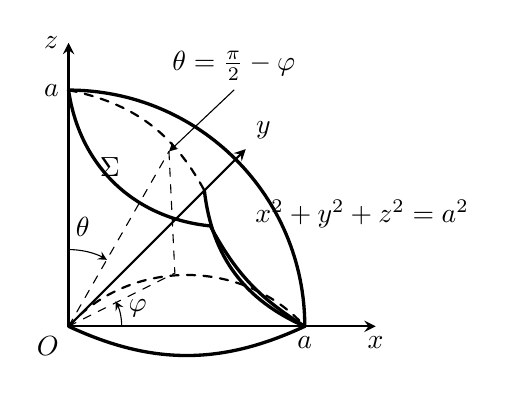
\begin{tikzpicture}[scale=1.5, >=stealth, line cap=round, line join=round]
    % 原点
    \coordinate (O) at (0,0);
    \node[below left] at (O) {$O$};
    
    % 坐标轴
    % z 轴向上
    \draw[->, thick] (0,0) -- (0,2.4) node[left] {$z$};
    % x 轴向右
    \draw[->, thick] (0,0) -- (2.6,0) node[below] {$x$};
    % y 轴向斜右上 (约 45 度)
    \draw[->, thick] (0,0) -- (1.5,1.5) node[above right] {$y$};
    
    % 球面在第一卦限的大圆轮廓
    % xOz 平面内圆弧 (半径 a = 2.0)
    \draw[very thick] (2.0,0) arc (0:90:2.0);
    \node[left] at (0,2.0) {$a$};
    \node[below] at (2.0,0) {$a$};
    
    % yOz 平面内的球面大圆弧 (虚线透视)
    \draw[dashed, thick] (0,2.0) to[bend left=25] (1.15,1.15);
    
    % xOy 平面内赤道大圆弧
    \draw[very thick] (2.0,0) to[bend left=30] (1.15,1.15);
    
    % 底面上柱面 x^2+y^2=ax 的半圆弧 (以 (1.0, 0) 为圆心，半径 1.0)
    \draw[dashed, thick] (0,0) to[bend left=48] (2.0,0);
    \draw[very thick] (0,0) to[bend right=25] (2.0,0);
    
    % 空间交线曲线: 球面与圆柱面交线 (在第一卦限的马鞍形空间拱线)
    % 从 (0,a) 到 (a,0) 弯曲
    \draw[very thick] (0,2.0) to[bend right=38] (1.2,0.85) to[bend right=15] (2.0,0);
    
    % 空间截面曲面片 Sigma 标注
    \node at (0.35,1.35) {$\Sigma$};
    
    % 球坐标辅助线与夹角 theta, phi:
    % 柱面上某一对应点 P
    \coordinate (P) at (0.85, 1.48);
    \coordinate (Pbot) at (0.90, 0.45);
    \draw[dashed] (P) -- (Pbot);
    \draw[dashed] (O) -- (P);
    \draw[dashed] (O) -- (Pbot);
    
    % 夹角 phi (在底面)
    \draw[->] (0.45,0) arc (0:28:0.45);
    \node[above right=-1pt] at (0.45,0.02) {$\varphi$};
    
    % 夹角 theta (与 z 轴夹角)
    \draw[->] (0,0.65) arc (90:60:0.65);
    \node[above] at (0.12,0.68) {$\theta$};
    
    % 方程指引关系
    \draw[<-] (P) -- (1.4, 2.0) node[above] {$\theta = \frac{\pi}{2} - \varphi$};
    \node[right] at (1.5, 0.95) {$x^{2}+y^{2}+z^{2}=a^{2}$};
  \end{tikzpicture}
  \caption{}\label{fig:11.1.7}
\end{figure}

\begin{example}\label{ex:11.1.6}
计算环面 $\Sigma: \boldsymbol{x}(\theta, \varphi)=((b+a \cos \theta) \cos \varphi,(b+a \cos \theta) \sin \varphi, a \sin \theta)$, $0 \leqslant \theta, \varphi \leqslant 2 \pi\ (0<a<b)$ 的表面积 $\sigma(\Sigma)$ (\cref{fig:11.1.8}).
\end{example}

\begin{solution}
\[
  \boldsymbol{x}_{\theta}^{\prime}=\left(-a \sin \theta \cos \varphi,-a \sin \theta \sin \varphi, a \cos \theta\right),
\]
\[
  \boldsymbol{x}_{\varphi}^{\prime}=\left(-(b+a \cos \theta) \sin \varphi,(b+a \cos \theta) \cos \varphi, 0\right),
\]
\[
  E=\boldsymbol{x}_{\theta}^{\prime} \cdot \boldsymbol{x}_{\theta}^{\prime}=a^{2}, \quad F=\boldsymbol{x}_{\theta}^{\prime} \cdot \boldsymbol{x}_{\varphi}^{\prime}=0\ \left(\boldsymbol{x}_{\theta}^{\prime} \perp \boldsymbol{x}_{\varphi}^{\prime}\right),
\]
\[
  G=\boldsymbol{x}_{\varphi}^{\prime} \cdot \boldsymbol{x}_{\varphi}^{\prime}=(b+a \cos \theta)^{2}.
\]
由此得到
\begin{align*}
  \sigma(\Sigma) &=\iint_{\substack{0 \leqslant \theta \leqslant 2 \pi \\ 0 \leqslant \varphi \leqslant 2 \pi}} \sqrt{E G-F^{2}}\,\mathrm{d} \theta \mathrm{d} \varphi \\
  &=\int_{0}^{2 \pi} \mathrm{d} \varphi \int_{0}^{2 \pi} a(b+a \cos \theta)\,\mathrm{d} \theta=2 \pi a\left(2 \pi b+a \sin \theta\bigg|_{0} ^{2 \pi}\right) \\
  &=4 \pi^{2} a b. \qedhere
\end{align*}
\end{solution}

\begin{figure}[htbp]
  \centering
  \begin{tikzpicture}[scale=1.45, >=stealth, line cap=round, line join=round]
    % 坐标轴
    \draw[->, thick] (-0.8,0) -- (3.6,0) node[below] {$x$};
    \draw[->, thick] (0,-1.5) -- (0,1.8) node[left] {$y$};
    \node[below left] at (0,0) {$O$};
    
    % 生成圆: 中心在 (b,0)，半径为 a (取 b=2.0, a=0.95)
    \coordinate (C) at (2.0,0);
    \draw[very thick] (C) circle (0.95);
    \node[below] at (2.0,0) {$b$};
    
    % 半径线段与角度 theta
    \coordinate (P) at ($(C) + (48:0.95)$);
    \draw[very thick] (C) -- (P);
    
    % 半径长 a 标注
    \node[above left] at ($(C)!0.55!(P)$) {$a$};
    
    % 夹角 theta
    \draw[->] (2.35,0) arc (0:48:0.35);
    \node[right] at (2.35,0.15) {$\theta$};
    
    % 圆方程标注
    \node[above right] at (1.65,0.98) {$(x-b)^{2}+y^{2}=a^{2}$};
  \end{tikzpicture}
  \caption{}\label{fig:11.1.8}
\end{figure}

\begin{example}\label{ex:11.1.7}
计算摆线一拱 $(x, y)=(a(t-\sin t), a(1-\cos t)), 0 \leqslant t \leqslant 2 \pi$ 绕 $x$ 轴旋转一周所得曲面 $\Sigma$ 的面积 $\sigma(\Sigma)$ (见第一册\extref{图 6.6.4}).
\end{example}

\begin{solution}[解法 1]
设摆线一拱为 $C$, 则
\begin{align*}
  \sigma(\Sigma) &=\int_{C} 2 \pi y\,\mathrm{d} s=2 \pi \int_{0}^{2 \pi} a(1-\cos t) \sqrt{\left[x^{\prime}(t)\right]^{2}+\left[y^{\prime}(t)\right]^{2}}\,\mathrm{d} t \\
  &=2 \pi a \int_{0}^{2 \pi}(1-\cos t) \sqrt{a^{2}(1-\cos t)^{2}+a^{2} \sin ^{2} t}\,\mathrm{d} t \\
  &=2 \pi a^{2} \int_{0}^{2 \pi}(1-\cos t) \sqrt{2(1-\cos t)}\,\mathrm{d} t=8 \pi a^{2} \int_{0}^{2 \pi} \sin ^{3} \frac{t}{2}\,\mathrm{d} t \\
  &=16 \pi a^{2} \int_{0}^{2 \pi}\left(\cos ^{2} \frac{t}{2}-1\right) \mathrm{d} \cos \frac{t}{2}=16 \pi a^{2}\left(\frac{\cos ^{3} \frac{t}{2}}{3}-\cos \frac{t}{2}\right)\bigg|_{0} ^{2 \pi}=\frac{64}{3} \pi a^{2}. \qedhere
\end{align*}
\end{solution}

\begin{solution}[解法 2]
旋转曲面 $\Sigma$ 的参数表示为
\begin{align*}
  \boldsymbol{x}(t, \varphi) &=(x(t, \varphi), y(t, \varphi), z(t, \varphi)) \\
  &=(a(t-\sin t), a(1-\cos t) \cos \varphi, a(1-\cos t) \sin \varphi), \\
  &\quad 0 \leqslant t \leqslant 2 \pi, \quad 0 \leqslant \varphi \leqslant 2 \pi.
\end{align*}
\[
  \boldsymbol{x}_{t}^{\prime}=(a(1-\cos t), a \sin t \cos \varphi, a \sin t \sin \varphi),
\]
\[
  \boldsymbol{x}_{\varphi}^{\prime}=(0,-a(1-\cos t) \sin \varphi, a(1-\cos t) \cos \varphi).
\]
\[
  E=\boldsymbol{x}_{t}^{\prime} \cdot \boldsymbol{x}_{t}^{\prime}=a^{2}\left[(1-\cos t)^{2}+\sin ^{2} t\right]=2 a^{2}(1-\cos t),
\]
\[
  F=\boldsymbol{x}_{t}^{\prime} \cdot \boldsymbol{x}_{\varphi}^{\prime}=0 \quad\left(\boldsymbol{x}_{t}^{\prime} \perp \boldsymbol{x}_{\varphi}^{\prime}\right).
\]
\[
  G=\boldsymbol{x}_{\varphi}^{\prime} \cdot \boldsymbol{x}_{\varphi}^{\prime}=a^{2}(1-\cos t)^{2}.
\]
\begin{align*}
  \sigma(\Sigma) &=\iint_{\substack{0 \leqslant t \leqslant 2 \pi \\ 0 \leqslant \varphi \leqslant 2 \pi}} \sqrt{E G-F^{2}}\,\mathrm{d} t \mathrm{d} \varphi=\iint_{\substack{0 \leqslant t \leqslant 2 \pi \\ 0 \leqslant \varphi \leqslant 2 \pi}} \sqrt{2} a^{2} \sqrt{(1-\cos t)^{3}}\,\mathrm{d} t \mathrm{d} \varphi \\
  &=4 a^{2} \int_{0}^{2 \pi} \sin ^{3} \frac{t}{2}\,\mathrm{d} t \int_{0}^{2 \pi} \mathrm{d} \varphi=8 \pi a^{2} \int_{0}^{2 \pi} \sin ^{3} \frac{t}{2}\,\mathrm{d} t=\frac{64}{3} \pi a^{2}. \qedhere
\end{align*}
\end{solution}

\begin{example}\label{ex:11.1.8}
将抛物线 $C: y=\sqrt{x}, 0 \leqslant x \leqslant a$ 绕 $x$ 轴旋转一周得旋转抛物面 $\Sigma$, 求它的面积 $\sigma(\Sigma)$.
\end{example}

\begin{solution}[解法 1]
\begin{align*}
  \sigma(\Sigma) &=\int_{C} 2 \pi y\,\mathrm{d} s=2 \pi \int_{0}^{a} \sqrt{x} \sqrt{1+\left[y^{\prime}(x)\right]^{2}}\,\mathrm{d} x \\
  &=2 \pi \int_{0}^{a} \sqrt{x} \sqrt{1+\frac{1}{4 x}}\,\mathrm{d} x=2 \pi \int_{0}^{a} \sqrt{x+\frac{1}{4}}\,\mathrm{d} x \\
  &=2 \pi \cdot \frac{2}{3}\left(x+\frac{1}{4}\right)^{\frac{3}{2}}\bigg|_{0} ^{a}=\frac{4 \pi}{3}\left[\left(a+\frac{1}{4}\right)^{\frac{3}{2}}-\frac{1}{8}\right] \\
  &=\frac{\pi}{6}\left[(4 a+1)^{\frac{3}{2}}-1\right]. \qedhere
\end{align*}
\end{solution}

\begin{solution}[解法 2]
旋转抛物面的参数表示为
\[
  \boldsymbol{x}(x, \varphi)=\left(x, \sqrt{x} \cos \varphi, \sqrt{x} \sin \varphi\right), \quad 0 \leqslant x \leqslant a,\ 0 \leqslant \varphi \leqslant 2 \pi.
\]
\[
  \boldsymbol{x}_{x}^{\prime}=\left(1, \frac{1}{2 \sqrt{x}} \cos \varphi, \frac{1}{2 \sqrt{x}} \sin \varphi\right),
\]
\[
  \boldsymbol{x}_{\varphi}^{\prime}=(0,-\sqrt{x} \sin \varphi, \sqrt{x} \cos \varphi).
\]
\[
  E=\boldsymbol{x}_{x}^{\prime} \cdot \boldsymbol{x}_{x}^{\prime}=1+\frac{1}{4 x},
\]
\[
  F=\boldsymbol{x}_{x}^{\prime} \cdot \boldsymbol{x}_{\varphi}^{\prime}=0 \quad\left(\boldsymbol{x}_{x}^{\prime} \perp \boldsymbol{x}_{\varphi}^{\prime}\right),
\]
\[
  G=\boldsymbol{x}_{\varphi}^{\prime} \cdot \boldsymbol{x}_{\varphi}^{\prime}=x.
\]
\begin{align*}
  \sigma(\Sigma) &=\iint_{\substack{0 \leqslant x \leqslant a \\ 0 \leqslant \varphi \leqslant 2 \pi}} \sqrt{E G-F^{2}}\,\mathrm{d} x \mathrm{d} \varphi=\iint_{\substack{0 \leqslant x \leqslant a \\ 0 \leqslant \varphi \leqslant 2 \pi}} \sqrt{x+\frac{1}{4}}\,\mathrm{d} x \mathrm{d} \varphi \\
  &=\int_{0}^{2 \pi} \mathrm{d} \varphi \int_{0}^{a} \sqrt{x+\frac{1}{4}}\,\mathrm{d} x \reason{由解法 1} \frac{\pi}{6}\left[(4 a+1)^{\frac{3}{2}}-1\right]. \qedhere
\end{align*}
\end{solution}

下面考虑一般的旋转曲面.

\begin{example}\label{ex:11.1.9}
将 $x O y$ 平面上的曲线 $C:(x, y)=(x(t), y(t)), \alpha \leqslant t \leqslant \beta$ 绕 $x$ 轴旋转一周得旋转曲面 $\Sigma$, 其中 $x(t), y(t)$ 都为 $C^{1}$ 函数. 求它的面积 $\sigma(\Sigma)$.
\end{example}

\begin{solution}[解法 1]
\[
  \sigma(\Sigma)=\int_{C} 2 \pi y\,\mathrm{d} s=2 \pi \int_{\alpha}^{\beta} y(t) \sqrt{\left[x^{\prime}(t)\right]^{2}+\left[y^{\prime}(t)\right]^{2}}\,\mathrm{d} t. \qedhere
\]
\end{solution}

\begin{solution}[解法 2]
旋转曲面 $\Sigma$ 的参数表示为
\[
  \boldsymbol{x}(t, \varphi)=(x(t), y(t) \cos \varphi, y(t) \sin \varphi), \quad \alpha \leqslant t \leqslant \beta,\ 0 \leqslant \varphi \leqslant 2 \pi.
\]
\[
  \boldsymbol{x}_{t}^{\prime}=\left(x^{\prime}(t), y^{\prime}(t) \cos \varphi, y^{\prime}(t) \sin \varphi\right),
\]
\[
  \boldsymbol{x}_{\varphi}^{\prime}=(0,-y(t) \sin \varphi, y(t) \cos \varphi).
\]
\[
  E=\boldsymbol{x}_{t}^{\prime} \cdot \boldsymbol{x}_{t}^{\prime}=\left[x^{\prime}(t)\right]^{2}+\left[y^{\prime}(t)\right]^{2},
\]
\[
  F=\boldsymbol{x}_{t}^{\prime} \cdot \boldsymbol{x}_{\varphi}^{\prime}=0 \quad\left(\boldsymbol{x}_{t}^{\prime} \perp \boldsymbol{x}_{\varphi}^{\prime}\right),
\]
\[
  G=\boldsymbol{x}_{\varphi}^{\prime} \cdot \boldsymbol{x}_{\varphi}^{\prime}=y^{2}(t).
\]
\begin{align*}
  \sigma(\Sigma) &=\iint_{\substack{\alpha \leqslant t \leqslant \beta \\ 0 \leqslant \varphi \leqslant 2 \pi}} \sqrt{E G-F^{2}}\,\mathrm{d} t \mathrm{d} \varphi=\iint_{\substack{\alpha \leqslant t \leqslant \beta \\ 0 \leqslant \varphi \leqslant 2 \pi}} y(t) \sqrt{\left[x^{\prime}(t)\right]^{2}+\left[y^{\prime}(t)\right]^{2}}\,\mathrm{d} t \mathrm{d} \varphi \\
  &=\int_{0}^{2 \pi} \mathrm{d} \varphi \int_{\alpha}^{\beta} y(t) \sqrt{\left[x^{\prime}(t)\right]^{2}+\left[y^{\prime}(t)\right]^{2}}\,\mathrm{d} t=2 \pi \int_{\alpha}^{\beta} y(t) \sqrt{\left[x^{\prime}(t)\right]^{2}+\left[y^{\prime}(t)\right]^{2}}\,\mathrm{d} t. \qedhere
\end{align*}
\end{solution}

\begin{example}\label{ex:11.1.10}
计算 $\mathbb{R}^{n}$ 中以原点为中心 $a>0$ 为半径的 $n-1$ 维球面 $S^{n-1}(a)$ 的面积 $\sigma\left(S^{n-1}(a)\right)$.
\end{example}

\begin{solution}[解法 1]
应用 $n-1$ 维球面坐标变换
\[
  \left\{\begin{aligned}
    x_{1} &=a \cos \theta_{1}, \\
    x_{2} &=a \sin \theta_{1} \cos \theta_{2}, \\
    x_{3} &=a \sin \theta_{1} \sin \theta_{2} \cos \theta_{3}, \\
    & \vdots \\
    x_{n-1} &=a \sin \theta_{1} \sin \theta_{2} \sin \theta_{3} \cdots \sin \theta_{n-2} \cos \theta_{n-1}, \\
    x_{n} &=a \sin \theta_{1} \sin \theta_{2} \sin \theta_{3} \cdots \sin \theta_{n-2} \sin \theta_{n-1},
  \end{aligned}\right.
\]
\[
  0 \leqslant \theta_{1}, \theta_{2}, \cdots, \theta_{n-2} \leqslant \pi, \quad 0 \leqslant \theta_{n-1} \leqslant 2 \pi.
\]
读者可以证明 $n-1$ 维球面 $S^{n-1}(a)$ 的面积元为 (复习题 11 题 2)
\begin{align*}
  \mathrm{d} \sigma &=\sqrt{\operatorname{det}\begin{pmatrix}
      g_{11} & \cdots & g_{1, n-1} \\
      \vdots & & \vdots \\
      g_{n-1,1} & \cdots & g_{n-1, n-1}
    \end{pmatrix}}\,\mathrm{d} \theta_{1} \mathrm{d} \theta_{2} \cdots \mathrm{d} \theta_{n-1} \\
  &=a^{n-1} \sin ^{n-2} \theta_{1} \sin ^{n-3} \theta_{2} \cdots \sin \theta_{n-2}\,\mathrm{d} \theta_{1} \mathrm{d} \theta_{2} \cdots \mathrm{d} \theta_{n-1}.
\end{align*}
因此, $S^{n-1}(a)$ 的面积为
\begin{align*}
  \sigma\left(S^{n-1}(a)\right) &=\int_{\substack{0 \leqslant \theta_{1}, \theta_{2}, \cdots, \theta_{n-2} \leqslant \pi \\ 0 \leqslant \theta_{n-1} \leqslant 2 \pi}} a^{n-1} \sin ^{n-2} \theta_{1} \sin ^{n-3} \theta_{2} \cdots \sin \theta_{n-2}\,\mathrm{d} \theta_{1} \cdots \mathrm{d} \theta_{n-1} \\
  &=a^{n-1} \cdot n \int_{0}^{1} r^{n-1}\,\mathrm{d} r \int_{\substack{0 \leqslant \theta_{1}, \theta_{2}, \cdots, \theta_{n-2} \leqslant \pi \\ 0 \leqslant \theta_{n-1} \leqslant 2 \pi}} \sin ^{n-2} \theta_{1} \sin ^{n-3} \theta_{2} \cdots \sin \theta_{n-2}\,\mathrm{d} \theta_{1} \cdots \mathrm{d} \theta_{n-1} \\
  &=n a^{n-1} v\left(B_{n}(1)\right)=\left\{\begin{aligned}
      &2 k a^{2 k-1} \cdot \frac{\pi^{k}}{k!}, & & n=2 k, \\
      &(2 k-1) a^{2 k-2} \cdot \frac{2^{k} \pi^{k-1}}{(2 k-1)!!}, & & n=2 k-1
    \end{aligned}\right. \\
  &=\left\{\begin{aligned}
      &\frac{2 \pi^{k}}{(k-1)!} a^{2 k-1}, & & n=2 k, \\
      &\frac{2^{k} \pi^{k-1}}{(2 k-3)!!} a^{2 k-2}, & & n=2 k-1
    \end{aligned}\right. \\
  &=\frac{2 \pi^{\frac{n}{2}}}{\Gamma\left(\frac{n}{2}\right)} a^{n-1}. \qedhere
\end{align*}
\end{solution}

\begin{solution}[解法 2]
因为 $x_{1}^{2}+x_{2}^{2}+\cdots+x_{n}^{2}=a^{2},\ 2 x_{i}+2 x_{n} \cdot \frac{\partial x_{n}}{\partial x_{i}}=0$, 即
\[
  \frac{\partial x_{n}}{\partial x_{i}}=-\frac{x_{i}}{x_{n}}.
\]
所以 $S^{n-1}(a)$ 的上半球面可由方程
\[
  x_{n}=\sqrt{a^{2}-\left(x_{1}^{2}+x_{2}^{2}+\cdots+x_{n-1}^{2}\right)}, \quad x_{1}^{2}+x_{2}^{2}+\cdots+x_{n-1}^{2} \leqslant a^{2}
\]
确定. 于是,
\begin{align*}
  \sigma\left(S^{n-1}(a)\right) &=2 \idotsint_{x_{1}^{2}+x_{2}^{2}+\cdots+x_{n-1}^{2} \leqslant a^{2}} \sqrt{1+\left(\frac{\partial x_{n}}{\partial x_{1}}\right)^{2}+\cdots+\left(\frac{\partial x_{n}}{\partial x_{n-1}}\right)^{2}}\,\mathrm{d} x_{1} \cdots \mathrm{d} x_{n-1} \\
  &=2 \idotsint_{x_{1}^{2}+\cdots+x_{n-1}^{2} \leqslant a^{2}} \sqrt{1+\left(-\frac{x_{1}}{x_{n}}\right)^{2}+\cdots+\left(-\frac{x_{n-1}}{x_{n}}\right)^{2}}\,\mathrm{d} x_{1} \cdots \mathrm{d} x_{n-1} \\
  &=2 \idotsint_{x_{1}^{2}+\cdots+x_{n-1}^{2} \leqslant a^{2}} \frac{a}{x_{n}}\,\mathrm{d} x_{1} \cdots \mathrm{d} x_{n-1} \\
  &\reasonb{\extref{例 10.5.14}} {x_{i}=a y_{i},\ i=1,2, \cdots, n-1} 2 \idotsint_{y_{1}^{2}+\cdots+y_{n-1}^{2} \leqslant 1} \\
  &\quad \frac{a}{\sqrt{a^{2}-a^{2}\left(y_{1}^{2}+\cdots+y_{n-1}^{2}\right)}}\, a^{n-1}\,\mathrm{d} y_{1} \cdots \mathrm{d} y_{n-1} \\
  &=2 a^{n-1} \idotsint_{y_{1}^{2}+\cdots+y_{n-1}^{2} \leqslant 1} \frac{\mathrm{d} y_{1} \cdots \mathrm{d} y_{n-1}}{\sqrt{1-\left(y_{1}^{2}+\cdots+y_{n-1}^{2}\right)}}=a^{n-1} \sigma\left(S^{n-1}(1)\right) \\
  &\reason{\extref{例 10.5.14}}\left\{\begin{aligned}
      &\frac{2 \pi^{k}}{(k-1)!} a^{2 k-1}, & & n=2 k, \\
      &\frac{2^{k} \pi^{k-1}}{(2 k-3)!!} a^{2 k-2}, & & n=2 k-1
    \end{aligned}\right. \\
  &=\frac{2 \pi^{\frac{n}{2}}}{\Gamma\left(\frac{n}{2}\right)} a^{n-1}. \qedhere
\end{align*}
\end{solution}

\begin{example}\label{ex:11.1.11}
设 $\Sigma$ 为锥面 $z^{2}=k^{2}\left(x^{2}+y^{2}\right)(k>0)$ 被柱面 $x^{2}+y^{2}=2 a x$ 截下的部分. 计算曲面积分
\[
  \iint_{\Sigma}\left(y^{2} z^{2}+z^{2} x^{2}+x^{2} y^{2}\right) \mathrm{d} \sigma.
\]
\end{example}

\begin{solution}
设 $\Sigma$ 的上半部为
\[
  z=k \sqrt{x^{2}+y^{2}}, \quad x^{2}+y^{2} \leqslant 2 a x, \quad z>0,
\]
故面积元为
\[
  \mathrm{d} \sigma=\sqrt{1+\left(\frac{\partial z}{\partial x}\right)^{2}+\left(\frac{\partial z}{\partial y}\right)^{2}}\,\mathrm{d} x \mathrm{d} y=\sqrt{1+\frac{k^{2} x^{2}}{x^{2}+y^{2}}+\frac{k^{2} y^{2}}{x^{2}+y^{2}}}\,\mathrm{d} x \mathrm{d} y=\sqrt{1+k^{2}}\,\mathrm{d} x \mathrm{d} y.
\]
\begin{align*}
  \iint_{\Sigma} & \left(y^{2} z^{2}+z^{2} x^{2}+x^{2} y^{2}\right) \mathrm{d} \sigma \\
  &\reason{对称性} 4 \iint_{\substack{x^{2}+y^{2} \leqslant 2 a x \\ x, y \geqslant 0}}\left[\left(x^{2}+y^{2}\right) k^{2}\left(x^{2}+y^{2}\right)+x^{2} y^{2}\right] \sqrt{1+k^{2}}\,\mathrm{d} x \mathrm{d} y \\
  &=4 \sqrt{1+k^{2}} \iint_{\substack{x^{2}+y^{2} \leqslant 2 a x \\ x, y \geqslant 0}}\left[k^{2}\left(x^{2}+y^{2}\right)^{2}+x^{2} y^{2}\right] \mathrm{d} x \mathrm{d} y \\
  &\reason{极坐标变换} 4 \sqrt{1+k^{2}} \int_{0}^{\frac{\pi}{2}} \mathrm{d} \varphi \int_{0}^{2 a \cos \varphi}\left[k^{2} r^{4}+r^{4} \sin ^{2} \varphi \cos ^{2} \varphi\right] r\,\mathrm{d} r \\
  &=4 \sqrt{1+k^{2}} \int_{0}^{\frac{\pi}{2}}\left(k^{2}+\sin ^{2} \varphi \cos ^{2} \varphi\right) \frac{r^{6}}{6}\bigg|_{0} ^{2 a \cos \varphi} \mathrm{d} \varphi \\
  &=\frac{128 a^{6}}{3} \sqrt{1+k^{2}} \int_{0}^{\frac{\pi}{2}}\left(k^{2}+\sin ^{2} \varphi \cos ^{2} \varphi\right) \cos ^{6} \varphi\,\mathrm{d} \varphi \\
  &=\frac{128 a^{6}}{3} \sqrt{1+k^{2}} \int_{0}^{\frac{\pi}{2}}\left(k^{2} \cos ^{6} \varphi+\cos ^{8} \varphi-\cos ^{10} \varphi\right) \mathrm{d} \varphi \\
  &=\frac{128 a^{6}}{3} \sqrt{1+k^{2}}\left(k^{2} \cdot \frac{5 \times 3}{6 \times 4 \times 2}+\frac{7 \times 5 \times 3}{8 \times 6 \times 4 \times 2}-\frac{9 \times 7 \times 5 \times 3}{10 \times 8 \times 6 \times 4 \times 2}\right) \frac{\pi}{2} \\
  &=\frac{128 a^{6}}{3} \sqrt{1+k^{2}} \cdot \frac{5}{16}\left(k^{2}+\frac{7}{8}-\frac{63}{80}\right) \cdot \frac{\pi}{2}=\frac{\pi}{12}\left(80 k^{2}+7\right) \sqrt{1+k^{2}} a^{6}. \qedhere
\end{align*}
\end{solution}

\begin{example}\label{ex:11.1.12}
设 $\Sigma=\left\{(x, y, z) \mid x^{2}+y^{2}=a^{2},\ 0 \leqslant z \leqslant h\right\}$ 为圆柱面. 计算第一型曲面积分
\[
  \iint_{\Sigma}\left(x^{4}+y^{4}\right) \mathrm{d} \sigma.
\]
\end{example}

\begin{solution}
由于 $\Sigma$ 为圆柱面, 故采用柱面坐标变换
\[
  \boldsymbol{x}(\varphi, z)=(x, y, z)=(a \cos \varphi, a \sin \varphi, z).
\]
于是,
\[
  \boldsymbol{x}_{\varphi}^{\prime}=(-a \sin \varphi, a \cos \varphi, 0),
\]
\[
  \boldsymbol{x}_{z}^{\prime}=(0,0,1),
\]
\[
  E=\boldsymbol{x}_{\varphi}^{\prime} \cdot \boldsymbol{x}_{\varphi}^{\prime}=a^{2}, \quad F=\boldsymbol{x}_{\varphi}^{\prime} \cdot \boldsymbol{x}_{z}^{\prime}=0 \quad\left(\boldsymbol{x}_{\varphi}^{\prime} \perp \boldsymbol{x}_{z}^{\prime}\right), \quad G=\boldsymbol{x}_{z}^{\prime} \cdot \boldsymbol{x}_{z}^{\prime}=1.
\]
面积元为 $\mathrm{d} \sigma=\sqrt{E G-F^{2}}\,\mathrm{d} \varphi \mathrm{d} z=a\,\mathrm{d} \varphi \mathrm{d} z$. 从而第一型曲面积分
\begin{align*}
  \iint_{\Sigma} & \left(x^{4}+y^{4}\right) \mathrm{d} \sigma \reason{对称性} 2 \iint_{\Sigma} y^{4}\,\mathrm{d} \sigma \reason{柱面坐标变换} 2 \iint_{\substack{0 \leqslant \varphi \leqslant 2 \pi \\ 0 \leqslant z \leqslant h}} a^{4} \sin ^{4} \varphi \cdot a\,\mathrm{d} \varphi \mathrm{d} z \\
  &=8 a^{5} \int_{0}^{\frac{\pi}{2}} \sin ^{4} \varphi\,\mathrm{d} \varphi \cdot \int_{0}^{h} \mathrm{d} z=8 a^{5} h \cdot \frac{3 \cdot 1}{4 \cdot 2} \cdot \frac{\pi}{2}=\frac{3}{2} \pi h a^{5}. \qedhere
\end{align*}
\end{solution}

\begin{example}\label{ex:11.1.13}
设 $\Sigma=\left\{(x, y, z) \mid x^{2}+y^{2}+z^{2}=a^{2},\ z \geqslant 0\right\}$ 为半球面. 计算第一型曲面积分
\[
  \iint_{\Sigma}(x+y+z)\,\mathrm{d} \sigma.
\]
\end{example}

\begin{solution}
因为 $\int_{\Sigma} x\,\mathrm{d} \sigma \reason{$x$ 为奇函数} 0$, $\int_{\Sigma} y\,\mathrm{d} \sigma \reason{$y$ 为奇函数} 0$, 故
\begin{align*}
  \iint_{\Sigma}(x+y+z)\,\mathrm{d} \sigma &=\iint_{\Sigma} z\,\mathrm{d} \sigma=\iint_{x^{2}+y^{2} \leqslant a^{2}} z \sqrt{1+\left(\frac{\partial z}{\partial x}\right)^{2}+\left(\frac{\partial z}{\partial y}\right)^{2}}\,\mathrm{d} x \mathrm{d} y \\
  &=\iint_{x^{2}+y^{2} \leqslant a^{2}} z \sqrt{1+\left(-\frac{x}{z}\right)^{2}+\left(-\frac{y}{z}\right)^{2}}\,\mathrm{d} x \mathrm{d} y=\iint_{x^{2}+y^{2} \leqslant a^{2}} z \cdot \frac{a}{z}\,\mathrm{d} x \mathrm{d} y \\
  &=a \cdot \pi a^{2}=\pi a^{3}. \qedhere
\end{align*}
\end{solution}

\begin{example}\label{ex:11.1.14}
设 $S^{2}(a)$ 是以原点为中心 $a$ 为半径的球面, 即 $x^{2}+y^{2}+z^{2}=a^{2}$. 计算第一型曲面积分 $\iint_{S^{2}(a)} x^{2}\,\mathrm{d} \sigma$.
\end{example}

\begin{solution}[解法 1]
应用球面坐标, 有
\begin{align*}
  \iint_{S^{2}(a)} x^{2}\,\mathrm{d} \sigma &=\iint_{\substack{0 \leqslant \varphi \leqslant 2 \pi \\ 0 \leqslant \theta \leqslant \pi}} a^{2} \sin ^{2} \theta \cos ^{2} \varphi \cdot a^{2} \sin \theta\,\mathrm{d} \theta \mathrm{d} \varphi \\
  &=a^{4} \int_{0}^{2 \pi} \cos ^{2} \varphi\,\mathrm{d} \varphi \int_{0}^{\pi} \sin ^{3} \theta\,\mathrm{d} \theta=8 a^{4} \int_{0}^{\frac{\pi}{2}} \cos ^{2} \varphi\,\mathrm{d} \varphi \int_{0}^{\frac{\pi}{2}} \sin ^{3} \theta\,\mathrm{d} \theta \\
  &=8 a^{4} \cdot \frac{\pi}{4} \cdot \frac{2}{3}=\frac{4}{3} \pi a^{4}. \qedhere
\end{align*}
\end{solution}

\begin{solution}[解法 2]
由对称性显然有
\[
  \iint_{S^{2}(a)} x^{2}\,\mathrm{d} \sigma=\iint_{S^{2}(a)} y^{2}\,\mathrm{d} \sigma=\iint_{S^{2}(a)} z^{2}\,\mathrm{d} \sigma.
\]
将上面三式相加得到
\begin{align*}
  \iint_{S^{2}(a)} x^{2}\,\mathrm{d} \sigma &=\frac{1}{3} \iint_{S^{2}(a)}\left(x^{2}+y^{2}+z^{2}\right) \mathrm{d} \sigma=\frac{a^{2}}{3} \iint_{S^{2}(a)} \mathrm{d} \sigma=\frac{a^{2}}{3} \sigma\left(S^{2}(a)\right) \\
  &=\frac{a^{2}}{3} \cdot 4 \pi a^{2}=\frac{4}{3} \pi a^{4}. \qedhere
\end{align*}
\end{solution}

\begin{example}\label{ex:11.1.15}
设 $\Sigma$ 是球面 $x^{2}+y^{2}+z^{2}=a^{2}$ 被平面 $z=h\ (0<h<a)$ 所截的顶部 (\cref{fig:11.1.9}), 计算第一型曲面积分 $\iint_{\Sigma} \frac{\mathrm{d} \sigma}{z}$.
\end{example}

\begin{solution}
曲面 $\Sigma$ 的参数表示为 $\boldsymbol{x}(x, y)=(x, y, z)=(x, y, \sqrt{a^{2}-x^{2}-y^{2}})$, 其中 $\Delta=\{(x, y) \mid x^{2}+y^{2} \leqslant a^{2}-h^{2}\}$. 由于面积元
\[
  \mathrm{d} \sigma=\sqrt{1+\left(z_{x}^{\prime}\right)^{2}+\left(z_{y}^{\prime}\right)^{2}}\,\mathrm{d} x \mathrm{d} y=\frac{a}{\sqrt{a^{2}-x^{2}-y^{2}}}\,\mathrm{d} x \mathrm{d} y,
\]
所以,
\begin{align*}
  \iint_{\Sigma} \frac{\mathrm{d} \sigma}{z} &=\iint_{\Delta} \frac{1}{\sqrt{a^{2}-x^{2}-y^{2}}} \cdot \frac{a}{\sqrt{a^{2}-x^{2}-y^{2}}}\,\mathrm{d} x \mathrm{d} y \\
  &\reason{极坐标变换} a \int_{0}^{2 \pi} \mathrm{d} \varphi \int_{0}^{\sqrt{a^{2}-h^{2}}} \frac{r}{a^{2}-r^{2}}\,\mathrm{d} r \\
  &=-\pi a \ln \left(a^{2}-r^{2}\right)\bigg|_{0} ^{\sqrt{a^{2}-h^{2}}}=\pi a\left(\ln a^{2}-\ln h^{2}\right) \\
  &=2 \pi a \ln \frac{a}{h}. \qedhere
\end{align*}
\end{solution}

\begin{figure}[htbp]
  \centering
  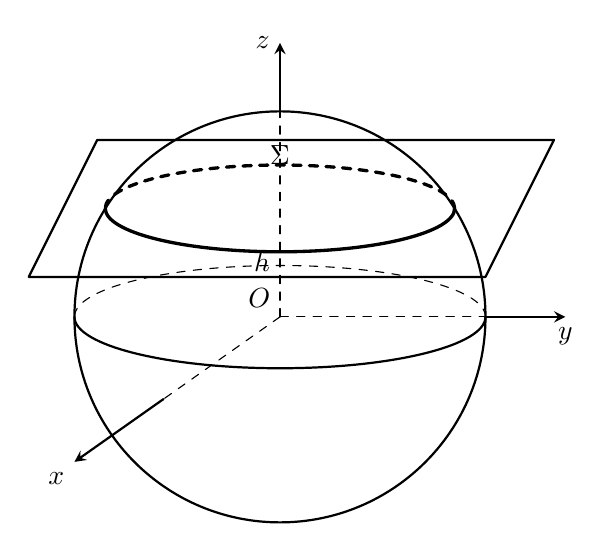
\begin{tikzpicture}[scale=1.45, >=stealth, line cap=round, line join=round]
    % 球面外轮廓圆
    \draw[thick] (0,0) circle (1.8);
    
    % 赤道椭圆: 后半虚线，前半实线
    \draw[dashed] (1.8,0) arc (0:180:1.8 and 0.45);
    \draw[thick] (-1.8,0) arc (180:360:1.8 and 0.45);
    
    % 坐标轴
    % z 轴
    \draw[dashed] (0,0) -- (0,1.8);
    \draw[->, thick] (0,1.8) -- (0,2.4) node[left] {$z$};
    
    % y 轴
    \draw[dashed] (0,0) -- (1.8,0);
    \draw[->, thick] (1.8,0) -- (2.5,0) node[below] {$y$};
    
    % x 轴 (左前约 215 度)
    \draw[dashed] (0,0) -- (-1.02,-0.72);
    \draw[->, thick] (-1.02,-0.72) -- (-1.8,-1.27) node[below left] {$x$};
    
    \node[above left] at (0,0) {$O$};
    
    % 水平截平面 z=h (高度 h = 0.95, 截圆半径 r = sqrt(1.8^2 - 0.95^2) = 1.53)
    % 切面板 (透视平行四边形)
    \draw[thick] (-2.2,0.95-0.6) -- (1.8,0.95-0.6) -- (2.4,0.95+0.6) -- (-1.6,0.95+0.6) -- cycle;
    
    % 截出的小圆 (截面椭圆: 后半虚线，前半实线)
    \draw[dashed, very thick] (1.53,0.95) arc (0:180:1.53 and 0.38);
    \draw[very thick] (-1.53,0.95) arc (180:360:1.53 and 0.38);
    
    % 截面高度 h 标注 (在 z 轴上)
    \node[left] at (0,0.48) {$h$};
    
    % 球冠截顶部分顶部标注 Sigma
    \node[above] at (0,1.25) {$\Sigma$};
  \end{tikzpicture}
  \caption{}\label{fig:11.1.9}
\end{figure}

\begin{example}\label{ex:11.1.16}
设 $\Sigma$ 为螺旋面 (\cref{fig:11.1.10}) 的一部分, 它的参数表示为
\begin{align*}
  \boldsymbol{x}(u, v) &=(x(u, v), y(u, v), z(u, v)) \\
  &=(u \cos v, u \sin v, v),
\end{align*}
\[
  (u, v) \in \Delta=[0, a] \times[0,2 \pi].
\]
计算第一型曲面积分 $\iint_{\Sigma} z\,\mathrm{d} \sigma$.
\end{example}

\begin{solution}
$\boldsymbol{x}_{u}^{\prime}=(\cos v, \sin v, 0)$,
\[
  \boldsymbol{x}_{v}^{\prime}=(-u \sin v, u \cos v, 1),
\]
\[
  E=\boldsymbol{x}_{u}^{\prime} \cdot \boldsymbol{x}_{u}^{\prime}=1,
\]
\[
  F=\boldsymbol{x}_{u}^{\prime} \cdot \boldsymbol{x}_{v}^{\prime}=0 \quad\left(\boldsymbol{x}_{u}^{\prime} \perp \boldsymbol{x}_{v}^{\prime}\right), \quad G=\boldsymbol{x}_{v}^{\prime} \cdot \boldsymbol{x}_{v}^{\prime}=1+u^{2}.
\]
于是,
\begin{align*}
  \iint_{\Sigma} z\,\mathrm{d} \sigma &=\iint_{\Delta} v \sqrt{E G-F^{2}}\,\mathrm{d} u \mathrm{d} v=\int_{0}^{a} \sqrt{1+u^{2}}\,\mathrm{d} u \int_{0}^{2 \pi} v\,\mathrm{d} v \\
  &=\left[\frac{u}{2} \sqrt{1+u^{2}}+\frac{1}{2} \ln \left(u+\sqrt{1+u^{2}}\right)\right]\bigg|_{0} ^{a} \cdot \frac{v^{2}}{2}\bigg|_{0} ^{2 \pi} \\
  &=\pi^{2}\left[a \sqrt{1+a^{2}}+\ln \left(a+\sqrt{1+a^{2}}\right)\right]. \qedhere
\end{align*}
\end{solution}

\begin{figure}[htbp]
  \centering
  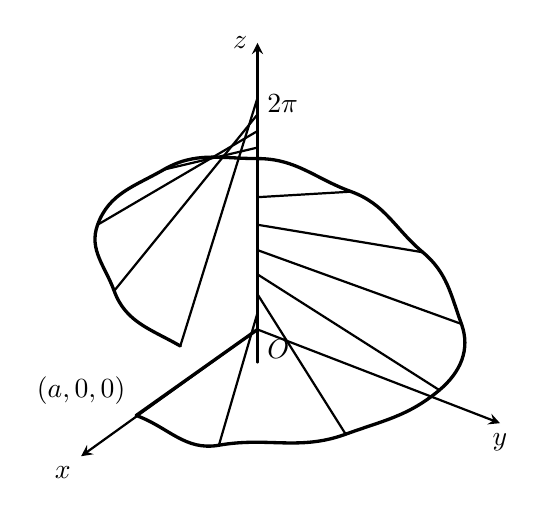
\begin{tikzpicture}[scale=1.4, >=stealth, line cap=round, line join=round]
    % 坐标轴
    % z 轴向上
    \draw[->, thick] (0,-0.3) -- (0,2.6) node[left] {$z$};
    % x 轴向左前 (约 215 度)
    \draw[->, thick] (0,0) -- (-1.6,-1.15) node[below left] {$x$};
    % y 轴向右下 (约 -30 度)
    \draw[->, thick] (0,0) -- (2.2,-0.85) node[below] {$y$};
    \node[below right] at (0,0) {$O$};
    
    % 螺旋面参数曲面片:
    % 从 x 轴上点 (a, 0, 0) 开始，绕 z 轴逆时针旋转上升一周 (0 <= v <= 2pi)
    % 辐射母线 (外端为螺旋线，内端在 z 轴)
    % 起点母线
    \coordinate (Start) at (-1.1,-0.78);
    \draw[very thick] (0,0) -- (Start) node[above left] {$(a,0,0)$};
    
    % 螺旋线上升轮廓 (用光滑贝塞尔曲线连接各母线外端点)
    % 采样辐射母线 (v = 0 到 360 度，对应 z 从 0 到 1.85)
    \coordinate (P0) at (-1.10, -0.78);
    \coordinate (P1) at (-0.35, -1.05);
    \coordinate (P2) at (0.80, -0.95);
    \coordinate (P3) at (1.65, -0.55);
    \coordinate (P4) at (1.85, 0.05);
    \coordinate (P5) at (1.50, 0.70);
    \coordinate (P6) at (0.85, 1.25);
    \coordinate (P7) at (0.00, 1.55);
    \coordinate (P8) at (-0.85, 1.45);
    \coordinate (P9) at (-1.45, 0.95);
    \coordinate (P10) at (-1.30, 0.35);
    \coordinate (P11) at (-0.70, -0.15);
    
    % 绘制辐射母线
    \draw[thick] (0,0.15) -- (P1);
    \draw[thick] (0,0.32) -- (P2);
    \draw[thick] (0,0.50) -- (P3);
    \draw[thick] (0,0.72) -- (P4);
    \draw[thick] (0,0.95) -- (P5);
    \draw[thick] (0,1.20) -- (P6);
    \draw[thick] (0,1.45) -- (P7);
    \draw[thick] (0,1.65) -- (P8);
    \draw[thick] (0,1.80) -- (P9);
    \draw[thick] (0,1.95) -- (P10);
    \draw[thick] (0,2.10) -- (P11);
    
    % 顶端母线与高度 2pi 标注
    \node[right] at (0,2.05) {$2\pi$};
    
    % 外边界螺旋线
    \draw[very thick] (P0) to[out=-20, in=190] (P1) to[out=10, in=200] (P2) to[out=20, in=220] (P3)
      to[out=40, in=-70] (P4) to[out=110, in=-40] (P5) to[out=140, in=-20] (P6)
      to[out=160, in=0] (P7) to[out=180, in=30] (P8) to[out=210, in=70] (P9)
      to[out=250, in=110] (P10) to[out=290, in=150] (P11);
      
    % 内轴线
    \draw[very thick] (0,0) -- (0,2.10);
  \end{tikzpicture}
  \caption{}\label{fig:11.1.10}
\end{figure}

\begin{exblock}{练习题 11.1}
\item 计算下列第一型曲线积分:
\begin{enumerate}[label=(\arabic*),leftmargin=2.6em,itemsep=0.15\baselineskip,topsep=0.2\baselineskip]
  \item $\int_{C}\left(x^{2}+y^{2}\right)^{n} \mathrm{d} s,\ C:\ (x, y)=(a \cos t, a \sin t),\ 0 \leqslant t \leqslant 2 \pi,\ n \in \mathbb{Z}_{+},\ a>0$;
  \item $\int_{C}(x+y)\,\mathrm{d} s,\ C$: 顶点为 $(0,0),(1,0),(0,1)$ 的三角形边界;
  \item $\int_{C} z\,\mathrm{d} s,\ C$: 圆锥螺线 $(x, y, z)=(t \cos t, t \sin t, t),\ t \in[0,2 \pi]$;
  \item $\int_{C} x^{2}\,\mathrm{d} s,\ C$: 圆周 $x^{2}+y^{2}+z^{2}=a^{2},\ x+y+z=0$;
  \item $\int_{C} z\,\mathrm{d} s,\ C:\ x^{2}+y^{2}=z^{2},\ y^{2}=a x$, 由 $(0,0,0)$ 到 $(a, a, \sqrt{2} a)$ 之间的一段, 其中 $a>0$;
  \item $\int_{C} y^{2}\,\mathrm{d} s,\ C$: 旋轮线的一拱, $(x, y)=(a(t-\sin t), a(1-\cos t)),\ 0 \leqslant t \leqslant 2 \pi$.
\end{enumerate}

\item 考察椭圆
\[
  \frac{x^{2}}{a^{2}}+\frac{y^{2}}{b^{2}}=1 \quad(a>b \geqslant 0),
\]
称
\[
  e=\sqrt{\frac{a^{2}-b^{2}}{a^{2}}}
\]
为该椭圆的离心率. 试通过 $e$ 和曲线积分来表示椭圆的周长.

\item 曲线 $C$ 用极坐标方程 $r=f(\varphi)(\alpha \leqslant \varphi \leqslant \beta)$ 所表示, 其中 $f$ 连续可导. 证明: $C$ 的长度为
\[
  \int_{\alpha}^{\beta} \sqrt{f^{2}(\varphi)+\left[f^{\prime}(\varphi)\right]^{2}}\,\mathrm{d} \varphi.
\]
利用这公式表达题 2 中椭圆的周长.

\item 计算下列曲面的面积:
\begin{enumerate}[label=(\arabic*),leftmargin=2.6em,itemsep=0.15\baselineskip,topsep=0.2\baselineskip]
  \item 锥面 $z=\sqrt{x^{2}+y^{2}}$ 被圆柱面 $x^{2}+y^{2}=2 x$ 截下的部分;
  \item 圆柱面 $x^{2}+z^{2}=a^{2}$ 被圆柱面 $x^{2}+y^{2}=a^{2}$ 截下的部分 $(a>0)$;
  \item 圆柱面介于平面 $x+z=0$ 与 $x-y=0$ 之间的部分;
  \item 球面 $x^{2}+y^{2}+z^{2}=a^{2}$ 被椭圆柱面
    \[
      \frac{x^{2}}{a^{2}}+\frac{y^{2}}{b^{2}}=1 \quad(0<b \leqslant a)
    \]
    所截下的部分;
  \item 马鞍面 $a z=x y$ 被圆柱面 $x^{2}+y^{2}=a^{2}$ 截下的部分 $(a>0)$;
  \item 抛物面 $x^{2}+y^{2}=2 a z$ 被柱面 $\left(x^{2}+y^{2}\right)^{2}=2 a^{2} x y$ 截下的部分 $(a>0)$;
  \item 螺旋面 $(x, y, z)=(r \cos \theta, r \sin \theta, h \theta),\ (r, \theta) \in(0, a) \times[0,2 \pi]$.
\end{enumerate}

\item 计算下列第一型曲面积分:
\begin{enumerate}[label=(\arabic*),leftmargin=2.6em,itemsep=0.15\baselineskip,topsep=0.2\baselineskip]
  \item $\iint_{\Sigma} \frac{\mathrm{d} \sigma}{(1+x+y)^{2}}$, 其中 $\Sigma$ 为四面体 $x+y+z \leqslant 1,\ x, y, z \geqslant 0$ 的边界;
  \item $\iint_{\Sigma}|x y z| \mathrm{d} \sigma,\ \Sigma:\ z=x^{2}+y^{2},\ z \leqslant 1$;
  \item $\iint_{\Sigma}(x y+y z+z x) \mathrm{d} \sigma,\ \Sigma:\ z=\sqrt{x^{2}+y^{2}}$ 被圆柱面 $x^{2}+y^{2}=2 x$ 割下的部分.
\end{enumerate}
\end{exblock}

\begin{exblock}{思考题 11.1}
\item 设 $\Sigma$ 为单位球面 $x^{2}+y^{2}+z^{2}=1$. 证明:
\[
  \iint_{\Sigma} f(a x+b y+c z)\,\mathrm{d} \sigma=2 \pi \int_{-1}^{1} f\left(\sqrt{a^{2}+b^{2}+c^{2}}\, t\right) \mathrm{d} t.
\]

\item 设 $\Sigma(t)$ 是平面 $x+y+z=t$ 被球面 $x^{2}+y^{2}+z^{2}=1$ 截下的部分, 且
\[
  F(x, y, z)=1-\left(x^{2}+y^{2}+z^{2}\right).
\]
证明: 对于 $|t| \leqslant \sqrt{3}$ 时, 有
\[
  \iint_{\Sigma(t)} F(x, y, z)\,\mathrm{d} \sigma=\frac{\pi}{18}\left(3-t^{2}\right).
\]

\item 对常数 $a>0$, 定义函数
\[
  f(x, y, z)=\left\{\begin{aligned}
    &1, & & x^{2}+y^{2}+z^{2} \leqslant a^{2}, \\
    &0, & & x^{2}+y^{2}+z^{2}>a^{2}.
  \end{aligned}\right.
\]
设 $\mathbb{R}^{3}$ 中的点 $(\xi, \eta, \zeta)$ 满足 $\xi^{2}+\eta^{2}+\zeta^{2}>a^{2}$, 计算第一型曲面积分
\[
  F(\xi, \eta, \zeta, t)=\iint_{\Sigma(t)} f(x, y, z)\,\mathrm{d} \sigma,
\]
其中 $\Sigma(t)$ 为球面 $(x-\xi)^{2}+(y-\eta)^{2}+(z-\zeta)^{2}=t^{2}$.

\item 设 $C$ 为右半 $y O z$ 平面中的 $C^{1}$ 简单曲线 $(y, z)=(\psi(u), \varphi(u)),\ a \leqslant u \leqslant b$. 让 $C$ 绕 $z$ 轴旋转一周得到旋转曲面 $\Sigma$, 其参数表示为
\begin{align*}
  \boldsymbol{x}(u, v) &=(x(u, v), y(u, v), z(u, v))=(\psi(u) \cos v, \psi(u) \sin v, \varphi(u)), \\
  & \quad a \leqslant u \leqslant b, \quad 0 \leqslant v \leqslant 2 \pi, \quad \psi(u)>0.
\end{align*}
求面积元 $\mathrm{d} \sigma$, 并证明 $\Sigma$ 的面积
\[
  \sigma(\Sigma)=2 \pi \int_{a}^{b} \psi(u) \sqrt{\left[\varphi^{\prime}(u)\right]^{2}+\left[\psi^{\prime}(u)\right]^{2}}\,\mathrm{d} u.
\]
\end{exblock}

% ==================================================================
%  §11.2  曲线、曲面及流形的定向
%  源：徐森林、薛春华《数学分析》第二册, 印刷页 322-332
%  底本：PaddleOCR-VL 为主, MinerU 交叉核对
%  约定：全西文标点; \[\] 表行间公式; align*/aligned 表多行;
%        定理/证明以 \qedhere 收 □, 不需 □ 的用 \noqedhere 抑制
%        章节标题（\chapter/\section）按原书原文保留顿号「、」,
%        正文一律不得出现中文标点（规范 §1.3）
%  图：图11.2.1-11.2.6、11.2.8-11.2.12、11.2.17 用 TikZ 绘;
%      图11.2.7、11.2.13、11.2.14（Möbius 带状图）与图11.2.15、11.2.16
%      （左右手系）TikZ 难以保真, 按规范 §5.1 用原书截图（figures/）。
%  按「原书优先」照录原书排版/笔误之处：
%      · 例11.2.1 中「由 $(-y,x)\perp(x,y)=\boldsymbol{x}$ 也可看出 ...」
%      · 例11.2.4 首行原书作 $\boldsymbol{x}'(\theta,z)$（带撇）
%      · 例11.2.5 中 $\boldsymbol{n}(\theta,0)$ 的行列式第三行首元素
%        原书印作 $-\sin\theta\cos\theta$（由结果反推应为 $\cos2\theta$）
%      · 定义11.2.4 条件 (3) 中原书印作 $\varphi_{n}^{\beta}$（应为 $u_{n}^{\beta}$）
%  订正 OCR 之处：
%      · 希腊字母 α 被 OCR 识成拉丁 a（已由原书影印页确认为 α）
%      · 「定义为」符号实为 \doteq（≐, 点上加于等号）
%      · \underset{\cdot}{连} 系 OCR 伪影, 实为「连续」
% ==================================================================
\section{曲线、曲面及流形的定向}

为了给出定向曲线上的第二型曲线积分, 定向曲面上的第二型曲面积分以及定向流形上的外微分形式的积分, 必须引进曲线, 曲面及流形可定向与定向的概念, 这是一个极其重要又是关键的概念. 它是由 Poincare 首先提出来的.

\begin{definition}\label{def:11.2.1}
设 $C$ 为空间 $\mathbb{R}^{n}$ 中的 $C^{1}$ 曲线. 如果沿 $C$ 有处处非零的连续变动的切向量场, 则称 $C$ 是可定向的 (\cref{fig:11.2.1}, 简记为\cref{fig:11.2.2}).
\end{definition}

\begin{figure}[htbp]
  \centering
  \begin{minipage}[b]{0.46\linewidth}
    \centering
    \begin{tikzpicture}[scale=1.15, >=stealth, line cap=round, line join=round]
      % 曲线 C 坐标轨迹 (三次贝塞尔曲线)
      \coordinate (P0) at (-2.0, -0.6);
      \coordinate (P1) at (-1.1,  0.55);
      \coordinate (P2) at (-0.2,  0.75);
      \coordinate (P3) at ( 0.6,  0.35);
      \coordinate (P4) at ( 1.3, -0.45);
      \coordinate (P5) at ( 2.0, -0.25);
      
      % 绘制光滑曲线 C
      \draw[very thick] plot[smooth, tension=0.85] coordinates {(P0) (P1) (P2) (P3) (P4) (P5)};
      \node[right] at (P5) {$C$};
      
      % 沿曲线取若干采样点，引出切向量场 tau (带箭头的切线向量)
      % 点 1: 约 P0 附近
      \coordinate (Q1) at (-1.60, -0.05);
      \draw[->, thick, ThemeColor] (Q1) -- ++(0.55, 0.45);
      \fill (Q1) circle (1.2pt);
      
      % 点 2: 约波峰 P2 附近
      \coordinate (Q2) at (-0.35, 0.74);
      \draw[->, thick, ThemeColor] (Q2) -- ++(0.70, 0.05);
      \fill (Q2) circle (1.2pt);
      
      % 点 3: 下坡段
      \coordinate (Q3) at (0.85, 0.05);
      \draw[->, thick, ThemeColor] (Q3) -- ++(0.55, -0.42);
      \fill (Q3) circle (1.2pt);
      
      % 点 4: 波谷回升段
      \coordinate (Q4) at (1.55, -0.40);
      \draw[->, thick, ThemeColor] (Q4) -- ++(0.60, 0.22);
      \fill (Q4) circle (1.2pt);
    \end{tikzpicture}
    \caption{}\label{fig:11.2.1}
  \end{minipage}\hfill
  \begin{minipage}[b]{0.46\linewidth}
    \centering
    \begin{tikzpicture}[scale=1.15, >=stealth, line cap=round, line join=round]
      % 同样的曲线 C，但带有曲线上嵌入的定向箭头
      \coordinate (P0) at (-2.0, -0.6);
      \coordinate (P1) at (-1.1,  0.55);
      \coordinate (P2) at (-0.2,  0.75);
      \coordinate (P3) at ( 0.6,  0.35);
      \coordinate (P4) at ( 1.3, -0.45);
      \coordinate (P5) at ( 2.0, -0.25);
      
      \draw[very thick, postaction={decorate}, decoration={markings,
        mark=at position 0.18 with {\arrow[thick]{>}},
        mark=at position 0.52 with {\arrow[thick]{>}},
        mark=at position 0.85 with {\arrow[thick]{>}}}]
        plot[smooth, tension=0.85] coordinates {(P0) (P1) (P2) (P3) (P4) (P5)};
      \node[right] at (P5) {$C$};
    \end{tikzpicture}
    \caption{}\label{fig:11.2.2}
  \end{minipage}
\end{figure}

如果 $C$ 有 $C^{1}$ 参数表示 $\boldsymbol{x}:[\alpha, \beta] \to \mathbb{R}^{n}$, 沿参数增加的方向或切向量场 $\boldsymbol{x}^{\prime}(t)$ 的指向确定了 $C$ 的一个定向, 记此定向曲线为 $\overrightarrow{C}$. 而参数减少的方向或 $-\boldsymbol{x}^{\prime}(t)$ 的指向确定了 $C$ 的另一个相反的定向, 记为 $\overrightarrow{C}^{-}$, 或称为 $\overrightarrow{C}$ 的负向. 如果参数定义域为 $[\alpha, \beta]$, 则 $f([\alpha, \beta])$ 为\textbf{道路连通集}, 所以 $C$ 恰有两个上述相反的定向.

如果 $C$ 由两个不相连接的道路连通部分, 则它恰有 4 个不同的定向.

\begin{example}\label{ex:11.2.1}
平面 $\mathbb{R}^{2}$ 上的圆 $C: x^{2}+y^{2}=R^{2}$.
\end{example}

参数表示为
\[
  \boldsymbol{x}(\theta)=(x(\theta), y(\theta))=(R \cos \theta, R \sin \theta), \quad 0 \leqslant \theta \leqslant 2 \pi,
\]
切向量场为
\[
  \boldsymbol{x}^{\prime}(\theta)=\left(x^{\prime}(\theta), y^{\prime}(\theta)\right)=(-R \sin \theta, R \cos \theta).
\]
从 $\theta=0$ 到 $\theta=2 \pi$ 确定了圆 $C$ 的一个定向, 它是逆时针方向的定向圆, 记为 $\overrightarrow{C}$ (\cref{fig:11.2.3}); 而从 $\theta=2 \pi$ 到 $\theta=0$ 确定了圆 $\overrightarrow{C}$ 的相反定向, 它是顺时针方向的定向圆, 记为 $\overrightarrow{C}^{-}$ (\cref{fig:11.2.4}).

实际上, 不用圆 $C$ 的参数表示, 由 $(-y, x) \perp(x, y)=\boldsymbol{x}$ 也可看出 $(-y, x)$ 是沿 $C$ 的逆时针方向的连续的单位切向量场 (当然处处非零). 而 $(-y, x)=(-R \sin \theta, R \cos \theta)$ 表明两种讨论的结果是一致的.

\begin{figure}[htbp]
  \centering
  \begin{minipage}[b]{0.48\linewidth}
    \centering
    \begin{tikzpicture}[scale=1.15, >=stealth, line cap=round, line join=round]
      % 坐标轴
      \draw[->] (-1.9, 0) -- (1.9, 0) node[below right] {$x$};
      \draw[->] (0, -1.8) -- (0, 1.8) node[right] {$y$};
      \node[below left] at (0,0) {$O$};
      
      % 定向圆 (逆时针箭头)
      \draw[thick, postaction={decorate}, decoration={markings,
        mark=at position 0.12 with {\arrow[thick]{>}},
        mark=at position 0.38 with {\arrow[thick]{>}},
        mark=at position 0.62 with {\arrow[thick]{>}},
        mark=at position 0.88 with {\arrow[thick]{>}}}]
        (0,0) circle (1.3);
      
      % 半径与点 P
      \coordinate (P) at (50:1.3);
      \draw (0,0) -- (P);
      \fill (P) circle (1.3pt);
      \node[right=2pt] at (P) {$\boldsymbol{x}=(R \cos \theta, R \sin \theta)$};
      
      % 切向量 (逆时针方向，垂直于半径 OP)
      \draw[->, very thick, ThemeColor] (P) -- ++(-0.95*0.766, 0.95*0.643) 
        node[above=2pt, inner sep=1pt] {$\boldsymbol{x}^{\prime}=(-R \sin \theta, R \cos \theta)$};
        
      % 直角符号
      \coordinate (A) at ($(P)!0.16!(0,0)$);
      \coordinate (B) at ($(P)!0.16!90:(0,0)$);
      \draw (A) -- ($(A)+(B)-(P)$) -- (B);
      
      % 夹角 theta
      \draw (0.40,0) arc (0:50:0.40);
      \node at (0.55,0.22) {$\theta$};
      \node[below] at (0.75, -0.05) {$R$};
      \node at (0, -2.15) {定向圆 $\overrightarrow{C}$};
    \end{tikzpicture}
    \caption{}\label{fig:11.2.3}
  \end{minipage}\hfill
  \begin{minipage}[b]{0.48\linewidth}
    \centering
    \begin{tikzpicture}[scale=1.15, >=stealth, line cap=round, line join=round]
      % 坐标轴
      \draw[->] (-1.9, 0) -- (1.9, 0) node[below right] {$x$};
      \draw[->] (0, -1.8) -- (0, 1.8) node[right] {$y$};
      \node[below left] at (0,0) {$O$};
      
      % 定向圆 (顺时针箭头)
      \draw[thick, postaction={decorate}, decoration={markings,
        mark=at position 0.12 with {\arrow[thick]{<}},
        mark=at position 0.38 with {\arrow[thick]{<}},
        mark=at position 0.62 with {\arrow[thick]{<}},
        mark=at position 0.88 with {\arrow[thick]{<}}}]
        (0,0) circle (1.3);
      
      % 半径与点 P
      \coordinate (P) at (50:1.3);
      \draw (0,0) -- (P);
      \fill (P) circle (1.3pt);
      \node[right=2pt] at (P) {$\boldsymbol{x}$};
      
      % 切向量 (顺时针方向，垂直于半径 OP)
      \draw[->, very thick, ThemeColor] (P) -- ++(0.95*0.766, -0.95*0.643);
      
      % 直角符号
      \coordinate (A) at ($(P)!0.16!(0,0)$);
      \coordinate (B) at ($(P)!0.16!-90:(0,0)$);
      \draw (A) -- ($(A)+(B)-(P)$) -- (B);
      
      % 夹角 theta
      \draw (0.40,0) arc (0:50:0.40);
      \node at (0.55,0.22) {$\theta$};
      \node[below] at (0.75, -0.05) {$R$};
      \node at (0, -2.15) {定向圆 $\overrightarrow{C}^{-}$};
    \end{tikzpicture}
    \caption{}\label{fig:11.2.4}
  \end{minipage}
\end{figure}

\begin{example}\label{ex:11.2.2}
$\mathbb{R}^{3}$ 中的圆柱螺线 $C: \boldsymbol{x}(\theta)=(x(\theta), y(\theta), z(\theta))=(R \cos \theta, R \sin \theta, b \theta)$, $R>0$, $b>0$.
\end{example}

切向量场
\[
  \boldsymbol{x}^{\prime}(\theta)=\left(x^{\prime}(\theta), y^{\prime}(\theta), z^{\prime}(\theta)\right)=(-R \sin \theta, R \cos \theta, b) \neq(0,0,0).
\]
当 $\theta$ 增加时, 它确定了圆柱螺线 $C$ 的一个定向, 记此定向曲线为 $\overrightarrow{C}$ (\cref{fig:11.2.5}); 当 $\theta$ 减少时, 它确定了圆柱螺线 $C$ 的一个相反方向, 记此定向曲线为 $\overrightarrow{C}^{-}$.

\begin{figure}[htbp]
  \centering
  \begin{tikzpicture}[scale=1.1, >=stealth, line cap=round, line join=round]
    % 上下两底面椭圆
    \draw[thick] (0, 2.1) ellipse (1.25 and 0.35);
    \draw[thick] (-1.25, -2.1) arc (180:360:1.25 and 0.35);
    \draw[dashed] (-1.25, -2.1) arc (180:0:1.25 and 0.35);
    
    % 两侧母线
    \draw[thick] (-1.25, 2.1) -- (-1.25, -2.1);
    \draw[thick] (1.25, 2.1) -- (1.25, -2.1);
    
    % 坐标轴: z 轴竖直向上
    \draw[dashed] (0, -2.1) -- (0, 2.1);
    \draw[->, thick] (0, 2.1) -- (0, 2.8) node[left] {$z$};
    
    % y 轴向右偏前
    \draw[dashed] (0, -2.1) -- (1.25, -2.1);
    \draw[->, thick] (1.25, -2.1) -- (2.2, -1.8) node[below] {$y$};
    
    % x 轴向左前
    \draw[dashed] (0, -2.1) -- (-0.8, -2.6);
    \draw[->, thick] (-0.8, -2.6) -- (-1.5, -3.1) node[below left] {$x$};
    \node[below right] at (0, -2.1) {$O$};
    
    % 圆柱螺线: 采用角度计算，避免弧度过大导致的 Dimension too large
    % 第一圈前段 (-90 到 90, 前侧实线)
    \draw[very thick]
      plot[domain=-90:90, samples=25, smooth, variable=\t] 
      ({1.25*sin(\t)}, {-2.1 + 0.95*(\t + 90)/180 + 0.35*cos(\t)});
    \draw[very thick, ->] ({1.25*sin(-5)}, {-2.1 + 0.95*85/180 + 0.35*cos(-5)}) -- 
                         ({1.25*sin(10)}, {-2.1 + 0.95*100/180 + 0.35*cos(10)});
      
    % 第一圈后段 (90 到 270, 后侧虚线)
    \draw[dashed, thick]
      plot[domain=90:270, samples=25, smooth, variable=\t] 
      ({1.25*sin(\t)}, {-1.15 + 0.95*(\t - 90)/180 - 0.35*cos(\t - 180)});
      
    % 第二圈前段 (前侧实线)
    \draw[very thick]
      plot[domain=-90:90, samples=25, smooth, variable=\t] 
      ({1.25*sin(\t)}, {-0.2 + 0.95*(\t + 90)/180 + 0.35*cos(\t)});
    \draw[very thick, ->] ({1.25*sin(-5)}, {-0.2 + 0.95*85/180 + 0.35*cos(-5)}) -- 
                         ({1.25*sin(10)}, {-0.2 + 0.95*100/180 + 0.35*cos(10)});
      
    % 第二圈后段 (后侧虚线)
    \draw[dashed, thick]
      plot[domain=90:270, samples=25, smooth, variable=\t] 
      ({1.25*sin(\t)}, {0.75 + 0.95*(\t - 90)/180 - 0.35*cos(\t - 180)});
      
    % 第三段到顶 (前侧实线)
    \draw[very thick]
      plot[domain=-90:0, samples=15, smooth, variable=\t] 
      ({1.25*sin(\t)}, {1.7 + 0.40*(\t + 90)/90 + 0.35*cos(\t)});
    \draw[very thick, ->] ({1.25*sin(-45)}, {1.7 + 0.40*45/90 + 0.35*cos(-45)}) -- 
                         ({1.25*sin(-30)}, {1.7 + 0.40*60/90 + 0.35*cos(-30)});

    % 方程标注
    \node[right] at (1.35, 0.4) {$\boldsymbol{x}(\theta)=(R \cos \theta, R \sin \theta, b \theta)$};
    \node[below] at (0, -3.2) {定向圆柱螺线 $\overrightarrow{C}$};
  \end{tikzpicture}
  \caption{}\label{fig:11.2.5}
\end{figure}

\begin{definition}\label{def:11.2.2}
$\mathbb{R}^{n}$ 中 $n-1$ 维超曲面的定向.

设 $\Sigma$ 为 $\mathbb{R}^{n}$ 中的 $n-1$ 维 $C^{1}$ 超曲面 (即 $n-1$ 维 $C^{1}$ 流形). 如果 $\Sigma$ 有连续变动的处处非零的法向量场, 则称曲面 $\Sigma$ 是可定向的 (\cref{fig:11.2.6}); 否则 $\Sigma$ 称为不可定向的 (\cref{fig:11.2.7}).
\end{definition}

显然, 如果 $\Sigma$ 上的一个处处非零的连续法向量场 $\boldsymbol{n}$ 确定了 $\Sigma$ 的一个定向, 记此定向曲面为 $\overrightarrow{\Sigma}$, 则 $-\boldsymbol{n}$ 确定了 $\Sigma$ 的另一个相反的定向, 记此定向曲面为 $\overrightarrow{\Sigma}^{-}$. 而道路连通 (这里等价于连通) 的超曲面 $\Sigma$ 恰有两个定向 (\cref{fig:11.2.6}).

\begin{figure}[htbp]
  \centering
  \begin{minipage}[b]{0.48\linewidth}
    \centering
    \begin{tikzpicture}[scale=1.1, >=stealth, line cap=round, line join=round]
      % 波浪形双侧曲面片
      \draw[thick] (-2.0, 0.1) .. controls (-1.3, 1.1) and (-0.6, 1.1) .. (0, 0.2)
                   .. controls (0.6, -0.6) and (1.3, 0.2) .. (2.0, -0.1);
      \draw[thick] (-2.0, -0.3) .. controls (-1.3, 0.7) and (-0.6, 0.7) .. (0, -0.2)
                   .. controls (0.6, -1.0) and (1.3, -0.2) .. (2.0, -0.5);
      \draw[thick] (-2.0, 0.1) -- (-2.0, -0.3);
      \draw[thick] (2.0, -0.1) -- (2.0, -0.5);
      
      % 连续法向量场 n
      \foreach \x/\y in {-1.3/0.82, -0.4/0.50, 0.7/0.05, 1.4/-0.02}{
        \draw[->, thick, ThemeColor] (\x,\y) -- ++(0.06, 0.65);
      }
      \node[above] at (-1.3, 1.5) {$\boldsymbol{n}$};
      \node[above] at (0.7, 0.75) {$\boldsymbol{n}$};
      \node[below] at (-1.5, -0.6) {$\overrightarrow{\Sigma}$};
      
      % 局部曲面片标注
      \node at (0, -1.35) {可定向曲面 (双侧曲面)};
    \end{tikzpicture}
    \caption{}\label{fig:11.2.6}
  \end{minipage}\hfill
  \begin{minipage}[b]{0.48\linewidth}
    \centering
    \includegraphics[width=0.92\linewidth]{ch11-fig-11.2.7}
    \caption{}\label{fig:11.2.7}
  \end{minipage}
\end{figure}

连通的可定向曲面也称为双侧曲面; 连通的不可定向曲面也称为单侧曲面. 注意, 如果 $\Sigma$ 有两个不相连接的道路连通部分, 且可定向, 则它恰有 4 个定向.

\begin{example}\label{ex:11.2.3}
球面 $\Sigma=S^{2}(R): F(x, y, z)=x^{2}+y^{2}+z^{2}-R^{2}=0$.
\end{example}

法向量场为 $\left(F_{x}^{\prime}, F_{y}^{\prime}, F_{z}^{\prime}\right)=(2 x, 2 y, 2 z)$. 从而 $\boldsymbol{n}_{\text{外}}=(x, y, z)$ 为球面 $\Sigma=S^{2}(R)$ 的一个处处非零的连续法向量场, 它确定了该球面的一个定向, 称为外法向 (外侧), 记作 $\overrightarrow{\Sigma}$ (\cref{fig:11.2.8}); 而 $\boldsymbol{n}_{\text{内}}=-\boldsymbol{n}_{\text{外}}=(-x,-y,-z)$ 确定了该球面的另一个相反定向, 称为内法向 (内侧), 记作 $\overrightarrow{\Sigma}^{-}$ (\cref{fig:11.2.9}).

\begin{figure}[htbp]
  \centering
  \begin{minipage}[b]{0.48\linewidth}
    \centering
    \begin{tikzpicture}[scale=1.15, >=stealth, line cap=round, line join=round]
      % 球面外轮廓与赤道圆
      \draw[thick] (0,0) circle (1.35);
      \draw[thick] (-1.35,0) arc (180:360:1.35 and 0.42);
      \draw[dashed] (-1.35,0) arc (180:0:1.35 and 0.42);
      
      % 坐标轴
      \draw[dashed] (0,0) -- (0,1.35);
      \draw[->, thick] (0,1.35) -- (0,2.0) node[above] {$z$};
      \draw[dashed] (0,0) -- (1.35,0);
      \draw[->, thick] (1.35,0) -- (2.0,0) node[right] {$y$};
      \node[below left] at (0,0) {$O$};
      
      % 球面上点 P 与外法向量
      \coordinate (P) at (45:1.35);
      \draw (0,0) -- (P);
      \fill (P) circle (1.3pt);
      \draw[->, very thick, ThemeColor] (P) -- ++(45:0.85) node[right] {$\boldsymbol{n}_{\text{外}}$};
      
      % 半径角
      \draw (0.35,0) arc (0:45:0.35);
      \node at (0.48,0.22) {$R$};
      \node at (0, -1.8) {外侧 $\overrightarrow{\Sigma}$};
    \end{tikzpicture}
    \caption{}\label{fig:11.2.8}
  \end{minipage}\hfill
  \begin{minipage}[b]{0.48\linewidth}
    \centering
    \begin{tikzpicture}[scale=1.15, >=stealth, line cap=round, line join=round]
      % 球面外轮廓与赤道圆
      \draw[thick] (0,0) circle (1.35);
      \draw[thick] (-1.35,0) arc (180:360:1.35 and 0.42);
      \draw[dashed] (-1.35,0) arc (180:0:1.35 and 0.42);
      
      % 坐标轴
      \draw[dashed] (0,0) -- (0,1.35);
      \draw[->, thick] (0,1.35) -- (0,2.0) node[above] {$z$};
      \draw[dashed] (0,0) -- (1.35,0);
      \draw[->, thick] (1.35,0) -- (2.0,0) node[right] {$y$};
      \node[below left] at (0,0) {$O$};
      
      % 球面上点 P 与内法向量
      \coordinate (P) at (45:1.35);
      \draw (0,0) -- (P);
      \fill (P) circle (1.3pt);
      \draw[->, very thick, ThemeColor] (P) -- ($(P)!0.65!(0,0)$) node[midway, left=2pt] {$\boldsymbol{n}_{\text{内}}$};
      
      % 半径角
      \draw (0.35,0) arc (0:45:0.35);
      \node at (0.48,0.22) {$R$};
      \node at (0, -1.8) {内侧 $\overrightarrow{\Sigma}^{-}$};
    \end{tikzpicture}
    \caption{}\label{fig:11.2.9}
  \end{minipage}
\end{figure}

因为球面 $\Sigma=S^{n}(R)$ 道路连通, 所以它恰有两个定向 (恰有两侧, 外侧与内侧). 蚂蚁能爬遍一侧, 但不能从一侧爬到另一侧.

应用球面坐标有
\begin{align*}
  \boldsymbol{x}(\theta, \varphi) &=(x(\theta, \varphi), y(\theta, \varphi), z(\theta, \varphi)) \\
                                 &=(R \sin \theta \cos \varphi, R \sin \theta \sin \varphi, R \cos \theta), \\
  \boldsymbol{x}_{\theta}^{\prime} &=(R \cos \theta \cos \varphi, R \cos \theta \sin \varphi,-R \sin \theta), \\
  \boldsymbol{x}_{\varphi}^{\prime} &=(-R \sin \theta \sin \varphi, R \sin \theta \cos \varphi, 0).
\end{align*}
法向量场为
\begin{align*}
  \boldsymbol{x}_{\theta}^{\prime} \times \boldsymbol{x}_{\varphi}^{\prime}
  &=\begin{vmatrix}
      \boldsymbol{e}_{1} & \boldsymbol{e}_{2} & \boldsymbol{e}_{3} \\
      R \cos \theta \cos \varphi & R \cos \theta \sin \varphi & -R \sin \theta \\
      -R \sin \theta \sin \varphi & R \sin \theta \cos \varphi & 0
    \end{vmatrix} \\
  &=\left(R^{2} \sin ^{2} \theta \cos \varphi, R^{2} \sin ^{2} \theta \sin \varphi, R^{2} \sin \theta \cos \theta\right) \\
  &=R^{2} \sin \theta(\sin \theta \cos \varphi, \sin \theta \sin \varphi, \cos \theta).
\end{align*}
当 $\theta=0, \pi$ 时, $\boldsymbol{x}_{\theta}^{\prime} \times \boldsymbol{x}_{\varphi}^{\prime}=\boldsymbol{0}$, 这是由于选择 $(\theta, \varphi)$ 作为参数造成``北极''与``南极''为奇异点. 但是,
\[
  \left(\frac{x}{R}, \frac{y}{R}, \frac{z}{R}\right)=(\sin \theta \cos \varphi, \sin \theta \sin \varphi, \cos \theta)=\boldsymbol{n}_{0}
\]
为球面 $\Sigma=S^{2}(R)$ 的连续的单位法向量场, 它确定了一个定向, 它就是外法向球面 $\overrightarrow{\Sigma}$.

\begin{example}\label{ex:11.2.4}
$\mathbb{R}^{3}$ 中柱面 $\Sigma: F(x, y, z)=x^{2}+y^{2}-R^{2}=0$.
\end{example}

法向量场为 $\left(F_{x}^{\prime}, F_{y}^{\prime}, F_{z}^{\prime}\right)=(2 x, 2 y, 0)$. 从而 $\boldsymbol{n}_{\text{外}}=(x, y, 0)$ 为柱面 $\Sigma$ 上的处处非零的连续法向量场, 它确定了该柱面的一个定向 (外侧) $\overrightarrow{\Sigma}$ (\cref{fig:11.2.10}); 而 $\boldsymbol{n}_{\text{内}}=-\boldsymbol{n}_{\text{外}}=(-x,-y,0)$ 确定了该柱面的另一个相反的定向 (内侧) $\overrightarrow{\Sigma}^{-}$ (\cref{fig:11.2.11}).

\begin{figure}[htbp]
  \centering
  \begin{minipage}[b]{0.48\linewidth}
    \centering
    \begin{tikzpicture}[scale=1.1, >=stealth, line cap=round, line join=round]
      % 柱面两端椭圆与母线
      \draw[thick] (0, 1.8) ellipse (1.1 and 0.32);
      \draw[thick] (-1.1, -1.8) arc (180:360:1.1 and 0.32);
      \draw[dashed] (-1.1, -1.8) arc (180:0:1.1 and 0.32);
      \draw[thick] (-1.1, 1.8) -- (-1.1, -1.8);
      \draw[thick] (1.1, 1.8) -- (1.1, -1.8);
      
      % 坐标轴
      \draw[dashed] (0, -1.8) -- (0, 1.8);
      \draw[->, thick] (0, 1.8) -- (0, 2.4) node[above] {$z$};
      \draw[->, thick] (0, 0) -- (1.8, 0.6) node[above right] {$y$};
      \node[below left] at (0,0) {$O$};
      
      % 外法向量 (向柱面外侧)
      \draw[->, very thick, ThemeColor] (-1.1, 0.2) -- ++(-0.75, 0) node[left] {$\boldsymbol{n}_{\text{外}}$};
      \draw[->, very thick, ThemeColor] (1.1, -0.4) -- ++(0.75, 0) node[right] {$\boldsymbol{n}_{\text{外}}$};
      
      \node at (0, -2.4) {外侧 $\overrightarrow{\Sigma}$};
    \end{tikzpicture}
    \caption{}\label{fig:11.2.10}
  \end{minipage}\hfill
  \begin{minipage}[b]{0.48\linewidth}
    \centering
    \begin{tikzpicture}[scale=1.1, >=stealth, line cap=round, line join=round]
      % 柱面两端椭圆与母线
      \draw[thick] (0, 1.8) ellipse (1.1 and 0.32);
      \draw[thick] (-1.1, -1.8) arc (180:360:1.1 and 0.32);
      \draw[dashed] (-1.1, -1.8) arc (180:0:1.1 and 0.32);
      \draw[thick] (-1.1, 1.8) -- (-1.1, -1.8);
      \draw[thick] (1.1, 1.8) -- (1.1, -1.8);
      
      % 坐标轴
      \draw[dashed] (0, -1.8) -- (0, 1.8);
      \draw[->, thick] (0, 1.8) -- (0, 2.4) node[above] {$z$};
      \draw[->, thick] (0, 0) -- (1.8, 0.6) node[above right] {$y$};
      \node[below left] at (0,0) {$O$};
      
      % 内法向量 (向柱面内部轴线)
      \draw[->, very thick, ThemeColor] (-1.1, 0.2) -- ++(0.70, 0) node[right] {$\boldsymbol{n}_{\text{内}}$};
      \draw[->, very thick, ThemeColor] (1.1, -0.4) -- ++(-0.70, 0) node[left] {$\boldsymbol{n}_{\text{内}}$};
      
      \node at (0, -2.4) {内侧 $\overrightarrow{\Sigma}^{-}$};
    \end{tikzpicture}
    \caption{}\label{fig:11.2.11}
  \end{minipage}
\end{figure}

因为柱面 $\Sigma$ 是道路连通的, 所以它恰有两个定向 (恰有两侧, 外侧与内侧). 蚂蚁能爬遍一侧, 但不能从一侧爬到另一侧.

应用柱面坐标有
\begin{align*}
  \boldsymbol{x}^{\prime}(\theta, z) &=(x(\theta, z), y(\theta, z), z(\theta, z))=(R \cos \theta, R \sin \theta, z), \\
  \boldsymbol{x}_{\theta}^{\prime} &=(-R \sin \theta, R \cos \theta, 0), \\
  \boldsymbol{x}_{z}^{\prime} &=(0,0,1).
\end{align*}
法向量场
\begin{align*}
  \boldsymbol{x}_{\theta}^{\prime} \times \boldsymbol{x}_{z}^{\prime}
  &=\begin{vmatrix}
      \boldsymbol{e}_{1} & \boldsymbol{e}_{2} & \boldsymbol{e}_{3} \\
      -R \sin \theta & R \cos \theta & 0 \\
      0 & 0 & 1
    \end{vmatrix} \\
  &=(R \cos \theta, R \sin \theta, 0)=(x, y, 0)=\boldsymbol{n}_{\text{外}}
\end{align*}
为该柱面上的处处非零的连续法向量场, 它确定了 $\overrightarrow{\Sigma}$ (外侧).

\begin{example}\label{ex:11.2.5}
Möbius 带 $\Sigma$.
\end{example}

不可定向的曲面的一个著名例子称为\textbf{Möbius 带}. 设想有一张矩形纸带 (\cref{fig:11.2.12}), 记作 $ABB_{1}A_{1}$, 用手捏着它的两头, 然后像拧麻花一样将它扭转过来, 再将线段 $AB$ 与线段 $A_{1}B_{1}$ 粘贴起来, 但要使 $A$ 与 $B_{1}$ 粘合, 而 $B$ 与 $A_{1}$ 粘合, 这样得到的曲面就称为 Möbius 带 (\cref{fig:11.2.13}). 记这张曲面为 $\Sigma$ 或 $M$.

\begin{figure}[htbp]
  \centering
  \begin{minipage}[b]{0.48\linewidth}
    \centering
    \begin{tikzpicture}[scale=1.1, >=stealth, line cap=round, line join=round]
      % 矩形纸带长条
      \draw[thick] (-2.2, -0.4) rectangle (2.2, 0.4);
      
      % 四个顶点标注
      \node[below left] at (-2.2, -0.4) {$A$};
      \node[above left] at (-2.2,  0.4) {$B$};
      \node[below right] at ( 2.2, -0.4) {$A_{1}$};
      \node[above right] at ( 2.2,  0.4) {$B_{1}$};
      
      % 两端弯折准备粘合的提示弯箭头
      % A 粘合到 B1，B 粘合到 A1
      \draw[->, thick, ThemeColor] (-2.2, 0.4) to[out=130, in=50] (-2.2, -0.4);
      \draw[->, thick, ThemeColor] ( 2.2, -0.4) to[out=-50, in=-130] ( 2.2, 0.4);
      
      \node at (0, -0.9) {矩形纸带 $ABB_{1}A_{1}$};
    \end{tikzpicture}
    \caption{}\label{fig:11.2.12}
  \end{minipage}\hfill
  \begin{minipage}[b]{0.48\linewidth}
    \centering
    \includegraphics[width=0.92\linewidth]{ch11-fig-11.2.13}
    \caption{}\label{fig:11.2.13}
  \end{minipage}
\end{figure}

在 $\Sigma$ 上任取一点 $P$, 在 $P$ 点处指定一个单位法向量, 当点 $P$ 在曲面 $\Sigma$ 上沿其中心线连续变化时, 这个单位法向量也连续地改变, 当点 $P$ 扫过一圈仍回到原来的出发点时, 这时的单位法向量的方向正好与最初的单位法向量的方向相反. 这就说明 Möbius 带是不可定向的 (严格证明应该用反证法), 即它是单侧曲面. 蚂蚁在 Möbius 带上无需越过它的边界就能爬遍所有的地方. 换另一种通俗的说法, 那就是, 有一个人提着红色油漆桶来刷 Möbius 带, 那么他可以将 Möbius 带的所有部分全都刷上红色油漆, 而无需越过它的边界. 对于双侧曲面 (如球面, 柱面等) 是绝对做不到的!

上述只是一种定性的描述, 就连连续变动的单位法向量场的描述也是不具体的. 现在我们给出 Möbius 带的一个参数表示, 并计算它的法向量场. Möbius 带的参数表示为
\begin{align*}
  \boldsymbol{x}(\theta, t) &=((1-t \sin \theta) \cos 2 \theta,(1-t \sin \theta) \sin 2 \theta, t \cos \theta) \\
                            &=(\cos 2 \theta, \sin 2 \theta, 0)+t(-\sin \theta \cos 2 \theta,-\sin \theta \sin 2 \theta, \cos \theta),
\end{align*}
\[
  0 \leqslant \theta \leqslant \pi, \quad|t| \leqslant h,
\]
其中 $h$ 为充分小的正数.
\begin{align*}
  \boldsymbol{x}_{\theta}^{\prime} &=(-2 \sin 2 \theta, 2 \cos 2 \theta, 0) \\
                                   &\quad +t(2 \sin \theta \sin 2 \theta-\cos \theta \cos 2 \theta,-2 \sin \theta \cos 2 \theta-\cos \theta \sin 2 \theta,-\sin \theta), \\
  \boldsymbol{x}_{t}^{\prime} &=(-\sin \theta \cos 2 \theta,-\sin \theta \sin 2 \theta, \cos \theta).
\end{align*}
\textbf{重点}\quad$\boldsymbol{x}(\pi, 0)=\boldsymbol{x}(0,0)$.

中心线 $t=0$, $\boldsymbol{x}(\theta, 0)=(\cos 2 \theta, \sin 2 \theta, 0)$ 为 $x O y$ 平面上的圆.

沿中心线的法向量场
\begin{align*}
  \boldsymbol{n}(\theta, 0) &=\boldsymbol{x}_{\theta}^{\prime}(\theta, 0) \times \boldsymbol{x}_{t}^{\prime}(\theta, 0) \\
                            &=(-2 \sin 2 \theta, 2 \cos 2 \theta, 0) \times(-\sin \theta \cos 2 \theta,-\sin \theta \sin 2 \theta, \cos \theta) \\
                            &=\begin{vmatrix}
                               \boldsymbol{e}_{1} & \boldsymbol{e}_{2} & \boldsymbol{e}_{3} \\
                               -2 \sin 2 \theta & 2 \cos 2 \theta & 0 \\
                               -\sin \theta \cos \theta & -\sin \theta \sin 2 \theta & \cos \theta
                             \end{vmatrix} \\
                            &=(2 \cos \theta \cos 2 \theta, 2 \sin 2 \theta \cos \theta, 2 \sin \theta).
\end{align*}
特别地
\[
  \boldsymbol{n}(0,0)=(0,2,0) \times(0,0,1)=(2,0,0),
\]
\[
  \boldsymbol{n}(\pi, 0)=(0,2,0) \times(0,0,-1)=(-2,0,0)=-\boldsymbol{n}(0,0),
\]
故沿中心线, 当 $\theta$ 从 0 连续变到 $\pi$ 时, 法向量 $\boldsymbol{n}(\theta, 0)$ 从 $\boldsymbol{n}(0,0)=(2,0,0)$ 连续变到 $\boldsymbol{n}(\pi, 0)=-\boldsymbol{n}(0,0)=(-2,0,0)$ (相反方向). 应用反证法可知 Möbius 带是不可定向的 (\cref{fig:11.2.14}).

\begin{definition}\label{def:11.2.3}
$\mathbb{R}^{n}$ 中 $n$ 维连通开集 $\Sigma$ 有两个定向, 一个是右手系 (\cref{fig:11.2.15}), 另一个是左手系 (\cref{fig:11.2.16}).
\end{definition}

\begin{figure}[htbp]
  \centering
  \includegraphics[width=0.52\linewidth]{ch11-fig-11.2.14}
  \caption{}\label{fig:11.2.14}
\end{figure}

\begin{figure}[htbp]
  \centering
  \begin{minipage}[b]{0.26\linewidth}
    \centering
    \includegraphics[width=\linewidth]{ch11-fig-11.2.15}
    \caption{}\label{fig:11.2.15}
  \end{minipage}\qquad
  \begin{minipage}[b]{0.29\linewidth}
    \centering
    \includegraphics[width=\linewidth]{ch11-fig-11.2.16}
    \caption{}\label{fig:11.2.16}
  \end{minipage}
\end{figure}

如果上述 $n$ 维开集有参数表示 $\boldsymbol{x}: \Delta \to \Sigma$, $\left(u_{1}, u_{2}, \cdots, u_{n}\right) \to \boldsymbol{x}\left(u_{1}, u_{2}, \cdots, u_{n}\right)=\left(x_{1}\left(u_{1}, u_{2}, \cdots, u_{n}\right), x_{2}\left(u_{1}, u_{2}, \cdots, u_{n}\right), \cdots, x_{n}\left(u_{1}, u_{2}, \cdots, u_{n}\right)\right)$, 则
\[
  \frac{\partial\left(x_{1}, x_{2}, \cdots, x_{n}\right)}{\partial\left(u_{1}, u_{2}, \cdots, u_{n}\right)}
  \begin{cases}
    >0, & \left(u_{1}, u_{2}, \cdots, u_{n}\right) \text{ 为右手系参数}, \\
    <0, & \left(u_{1}, u_{2}, \cdots, u_{n}\right) \text{ 为左手系参数}.
  \end{cases}
\]

回忆一下 $\mathbb{R}^{n}$ 中 $n-1$ 维 $C^{1}$ 正则超曲面 $\Sigma$, 它有参数表示 $\boldsymbol{x}(u_{1}, \allowbreak u_{2}, \allowbreak \cdots, \allowbreak u_{n-1})$, $(u_{1}, \allowbreak u_{2}, \allowbreak \cdots, \allowbreak u_{n-1}) \in \Delta$, $\operatorname{rank}\{\boldsymbol{x}_{u_{1}}^{\prime}, \allowbreak \boldsymbol{x}_{u_{2}}^{\prime}, \allowbreak \cdots, \allowbreak \boldsymbol{x}_{u_{n-1}}^{\prime}\}=n-1$. 因此, $\Sigma$ 上有处处非零的连续法向量场
\[
  \boldsymbol{x}_{u_{1}}^{\prime} \times \cdots \times \boldsymbol{x}_{u_{n-1}}^{\prime}
  =\begin{vmatrix}
     \boldsymbol{e}_{1} & \cdots & \boldsymbol{e}_{n} \\
     & \boldsymbol{x}_{u_{1}}^{\prime} & \\
     & \vdots & \\
     & \boldsymbol{x}_{u_{n-1}}^{\prime} &
   \end{vmatrix}.
\]
这就证明了 $\Sigma$ 是可定向的超曲面.

\begin{remark}\label{rem:11.2.1}
在\cref{ex:11.2.3}中, 读者千万不要误会从 $\boldsymbol{x}_{\theta}^{\prime} \times \boldsymbol{x}_{\varphi}^{\prime}$ 为 $S^{2}(R)$ 上的处处连续的法向量场就能导致 $S^{2}(R)$ 是可定向的, 原因是当 $\theta=0, \pi$ 时 $\boldsymbol{x}_{\theta}^{\prime} \times \boldsymbol{x}_{\varphi}^{\prime}=\boldsymbol{0}$, 它不是非零法向量! 用 $\theta, \varphi$ 作为 $S^{2}(R)$ 的参数, 它不满足正则超曲面整体参数表示的要求. 但是, 用这样的参数不行, 也不能否定 $S^{2}(R)$ 是可定向的. 事实上, 一眼就能看出 $(x, y, z)$ 是 $S^{2}(R)$ 上的处处非零的连续法向量场, 因而 $S^{2}(R)$ 是可定向的.

如果在 Möbius 带 $\Sigma$ (\cref{fig:11.2.13}) 上挖去一条直线段 $AB$ (与 $B_{1}A_{1}$ 粘合), 显然在余下的集合 $\Sigma \setminus AB$ 上有连续变动的处处非零的法向量场. 但是, 一旦当挖去的线段又粘合时, 发现两边的法向量方向恰好相反, 怎么也拼不起一个 $\Sigma$ 上的整体处处非零的连续法向量. 这是不可定向曲面几何上的特性.
\end{remark}

\begin{remark}\label{rem:11.2.2}
在\cref{def:11.2.1}中用处处非零的连续变动的切向量场来刻画一维曲线的可定向性. 在\cref{def:11.2.2}中用处处非零的连续变动的法向量场来刻画 $n-1$ 维超曲面的可定向性. 有一个问题自然会产生, 如何刻画 $k(2 \leqslant k \leqslant n-2)$ 维曲面的可定向性. 上述方法不能借鉴, 那么有什么新方法呢? 下面的定理给出了希望.
\end{remark}

\begin{theorem}\label{thm:11.2.1}
设 $\Sigma$ 为 $\mathbb{R}^{n}$ 中的 $n-1$ 维超曲面 (即 $n-1$ 维流形), 则

$\Sigma$ 上存在处处非零的连续法向量场 $\Leftrightarrow \Sigma$ 上存在局部坐标系族
\[
  \mathcal{D}_{1}=\left\{\left(U_{\alpha}, \varphi_{\alpha}\right),\left\{u_{i}^{\alpha} \mid i=1,2, \cdots, n-1\right\} \mid \alpha \in \mu\right\},
\]
使得

(1) $\bigcup\limits_{\alpha \in \mu} U_{\alpha}=\Sigma$;

(2) $U_{\alpha}$ 为 $\Sigma$ 中开集, $\varphi: U_{\alpha} \to \varphi_{\alpha}\left(U_{\alpha}\right)$, $x \to \varphi_{\alpha}(x)=(u_{1}^{\alpha}, \allowbreak u_{2}^{\alpha}, \allowbreak \cdots, \allowbreak u_{n-1}^{\alpha})$ 为同胚, 其中 $\varphi_{\alpha}\left(U_{\alpha}\right)$ 为 $\mathbb{R}^{n-1}$ 中的开集, $x=\varphi_{\alpha}^{-1}(u_{1}^{\alpha}, \allowbreak u_{2}^{\alpha}, \allowbreak \cdots, \allowbreak u_{n-1}^{\alpha})=(x_{1}(u_{1}^{\alpha}, \allowbreak u_{2}^{\alpha}, \allowbreak \cdots, \allowbreak u_{n-1}^{\alpha}), \allowbreak x_{2}(u_{1}^{\alpha}, \allowbreak u_{2}^{\alpha}, \allowbreak \cdots, \allowbreak u_{n-1}^{\alpha}), \allowbreak \cdots, \allowbreak x_{n}(u_{1}^{\alpha}, \allowbreak u_{2}^{\alpha}, \allowbreak \cdots, \allowbreak u_{n-1}^{\alpha}))$ 是 $C^{1}$ 的;

(3) $\forall\left(U_{\alpha}, \varphi_{\alpha}\right),\left\{u_{i}^{\alpha}\right\} \in \mathcal{D}_{1}$, $\forall\left(U_{\beta}, \varphi_{\beta}\right),\left\{u_{i}^{\beta}\right\} \in \mathcal{D}_{1}$, 如果 $U_{\alpha} \cap U_{\beta} \neq \varnothing$, 则坐标变换 $\varphi_{\beta} \circ \varphi_{\alpha}^{-1}: \varphi_{\alpha}\left(U_{\alpha} \cap U_{\beta}\right) \to \varphi_{\beta}\left(U_{\alpha} \cap U_{\beta}\right)$, $\left(u_{1}^{\alpha}, u_{2}^{\alpha}, \cdots, u_{n-1}^{\alpha}\right) \to\left(u_{1}^{\beta}, u_{2}^{\beta}, \cdots, u_{n-1}^{\beta}\right)$ 的 Jacobi 行列式
\[
  \frac{\partial\left(u_{1}^{\beta}, u_{2}^{\beta}, \cdots, u_{n-1}^{\beta}\right)}{\partial\left(u_{1}^{\alpha}, u_{2}^{\alpha}, \cdots, u_{n-1}^{\alpha}\right)}>0.
\]
\end{theorem}

\begin{proof}
$(\Rightarrow)$ 设 $\Sigma$ 上存在处处非零的连续法向量场 $\boldsymbol{n}$, $\left\{x_{i} \mid i=1,2, \cdots, n\right\}$ 为 $\mathbb{R}^{n}$ 中的通常的整体直角坐标. 取 $\Sigma$ 的连通的局部坐标系
\[
  \left(U_{\alpha}, \varphi_{\alpha}\right),\left\{u_{i}^{\alpha}\right\} \quad \text{与} \quad\left(U_{\beta}, \varphi_{\beta}\right),\left\{u_{i}^{\beta}\right\},
\]
使得
\[
  \left[\overrightarrow{x_{u_{1}^{\alpha}}^{\prime}}, x_{u_{2}^{\alpha}}^{\prime}, \cdots, x_{u_{n-1}^{\alpha}}^{\prime}, \boldsymbol{n}\right]=\left[\overrightarrow{e_{1}}, e_{2}, \cdots, e_{n}\right],
\]
即左边 $n$ 个向量用 $e_{1}, e_{2}, \cdots, e_{n}$ 表示的矩阵的行列式大于 0 (只要有一点满足此式, 则由 $U_{\alpha}$ 连通, $\boldsymbol{n}$ 连续与零值定值推出此式在 $U_{\alpha}$ 中成立), 其中 $\left\{e_{1}, e_{2}, \cdots, e_{n}\right\}$ 为 $\mathbb{R}^{n}$ 中关于直角坐标系 $\left\{x_{i}\right\}$ 的规范基向量场. 同理有
\[
  \left[\overrightarrow{x_{u_{1}^{\beta}}^{\prime}}, x_{u_{2}^{\beta}}^{\prime}, \cdots, x_{u_{n-1}^{\beta}}^{\prime}, \boldsymbol{n}\right]=\left[\overrightarrow{e_{1}}, e_{2}, \cdots, e_{n}\right],
\]
当 $U_{\alpha} \cap U_{\beta} \neq \varnothing$ 时, 在 $U_{\alpha} \cap U_{\beta}$ 中有
\[
  \begin{pmatrix}
    \boldsymbol{x}_{u_{1}^{\beta}}^{\prime} \\
    \vdots \\
    \boldsymbol{x}_{u_{n-1}^{\beta}}^{\prime} \\
    \boldsymbol{n}
  \end{pmatrix}
  =\begin{pmatrix}
    \dfrac{\partial u_{1}^{\alpha}}{\partial u_{1}^{\beta}} & \cdots & \dfrac{\partial u_{n-1}^{\alpha}}{\partial u_{1}^{\beta}} & 0 \\
    \vdots & & \vdots & \vdots \\
    \dfrac{\partial u_{1}^{\alpha}}{\partial u_{n-1}^{\beta}} & \cdots & \dfrac{\partial u_{n-1}^{\alpha}}{\partial u_{n-1}^{\beta}} & 0 \\
    0 & \cdots & 0 & 1
  \end{pmatrix}
  \begin{pmatrix}
    \boldsymbol{x}_{u_{1}^{\alpha}}^{\prime} \\
    \vdots \\
    \boldsymbol{x}_{u_{n-1}^{\alpha}}^{\prime} \\
    \boldsymbol{n}
  \end{pmatrix},
\]
故
\[
  \frac{\partial\left(u_{1}^{\alpha}, u_{2}^{\alpha}, \cdots, u_{n-1}^{\alpha}\right)}{\partial\left(u_{1}^{\beta}, u_{2}^{\beta}, \cdots, u_{n-1}^{\beta}\right)}
  =\operatorname{det}
  \begin{pmatrix}
    \dfrac{\partial u_{1}^{\alpha}}{\partial u_{1}^{\beta}} & \cdots & \dfrac{\partial u_{n-1}^{\alpha}}{\partial u_{1}^{\beta}} & 0 \\
    \vdots & & \vdots & \vdots \\
    \dfrac{\partial u_{1}^{\alpha}}{\partial u_{n-1}^{\beta}} & \cdots & \dfrac{\partial u_{n-1}^{\alpha}}{\partial u_{n-1}^{\beta}} & 0 \\
    0 & \cdots & 0 & 1
  \end{pmatrix}>0.
\]
于是,
\[
  \mathcal{D}_{1}=\left\{(U, \varphi),\left\{u_{i}\right\} \mid\left[\overrightarrow{x_{u_{1}^{\alpha}}^{\prime}}, x_{u_{2}^{\alpha}}^{\prime}, \cdots, x_{u_{n-1}^{\alpha}}^{\prime}, \boldsymbol{n}\right]=\left[\overrightarrow{e_{1}}, e_{2}, \cdots, e_{n}\right]\right\},
\]
为满足本定理右边三个条件的 $\Sigma$ 的局部坐标系族.

$(\Leftarrow)$ 设 $\mathcal{D}_{1}=\left\{\left(U_{\alpha}, \varphi_{\alpha}\right),\left\{u_{i}^{\alpha}\right\} \mid \alpha \in \mu\right\}$ 为 $\Sigma$ 上满足右边三个条件的局部坐标系族, $\left(U_{\alpha}, \varphi_{\alpha}\right),\left\{u_{i}^{\alpha}\right\} \in \mathcal{D}_{1}$,
\[
  \begin{pmatrix}
    \boldsymbol{x}_{u_{1}^{\alpha}}^{\prime} \\
    \vdots \\
    \boldsymbol{x}_{u_{n-1}^{\alpha}}^{\prime}
  \end{pmatrix}
  =\begin{pmatrix}
    \dfrac{\partial x_{1}}{\partial u_{1}^{\alpha}} & \cdots & \dfrac{\partial x_{n}}{\partial u_{1}^{\alpha}} \\
    \vdots & & \vdots \\
    \dfrac{\partial x_{1}}{\partial u_{n-1}^{\alpha}} & \cdots & \dfrac{\partial x_{n}}{\partial u_{n-1}^{\alpha}}
  \end{pmatrix}
  \begin{pmatrix}
    \boldsymbol{e}_{1} \\
    \vdots \\
    \boldsymbol{e}_{n}
  \end{pmatrix}.
\]
令
\begin{align*}
  n_{i}^{\alpha} &=(-1)^{i+n} \operatorname{det}
    \begin{pmatrix}
      \dfrac{\partial x_{1}}{\partial u_{1}^{\alpha}} & \cdots & \dfrac{\partial x_{i-1}}{\partial u_{1}^{\alpha}} & \dfrac{\partial x_{i+1}}{\partial u_{1}^{\alpha}} & \cdots & \dfrac{\partial x_{n}}{\partial u_{1}^{\alpha}} \\
      \vdots & & \vdots & \vdots & & \vdots \\
      \dfrac{\partial x_{1}}{\partial u_{n-1}^{\alpha}} & \cdots & \dfrac{\partial x_{i-1}}{\partial u_{n-1}^{\alpha}} & \dfrac{\partial x_{i+1}}{\partial u_{n-1}^{\alpha}} & \cdots & \dfrac{\partial x_{n}}{\partial u_{n-1}^{\alpha}}
    \end{pmatrix} \\
  &=(-1)^{i+n} \frac{\partial\left(x_{1}, \cdots, x_{i-1}, x_{i+1}, \cdots, x_{n}\right)}{\partial\left(u_{1}^{\alpha}, \cdots, u_{n-1}^{\alpha}\right)}, \quad i=1,2, \cdots, n.
\end{align*}
\[
  \boldsymbol{n}^{\alpha} \doteq \frac{\pm 1}{\sqrt{\sum_{i=1}^{n}\left(n_{i}^{\alpha}\right)^{2}}}\left(n_{1}^{\alpha}, n_{2}^{\alpha}, \cdots, n_{n}^{\alpha}\right),
\]
其中 $\pm 1$ 选得使
\[
  \left[\overrightarrow{x_{u_{1}^{\alpha}}^{\prime}, x_{u_{2}^{\alpha}}^{\prime}, \cdots, x_{u_{n-1}^{\alpha}}^{\prime}, \boldsymbol{n}^{\alpha}}\right]=\left[\overrightarrow{e_{1}, e_{2}, \cdots, e_{n}}\right],
\]
从 $\operatorname{rank}\left(\dfrac{\partial x_{i}}{\partial u_{j}^{\alpha}}\right)=\operatorname{rank}\left\{\boldsymbol{x}_{u_{1}^{\alpha}}^{\prime}, \boldsymbol{x}_{u_{2}^{\alpha}}^{\prime}, \cdots, \boldsymbol{x}_{u_{n-1}^{\alpha}}^{\prime}\right\}=n-1$ 可知, $\boldsymbol{n}^{\alpha}$ 是定义确切的. 又因为 $\dfrac{\partial x_{i}}{\partial u_{j}^{\alpha}}$ 为连续函数, 所以 $\boldsymbol{n}^{\alpha}$ 为 $U_{\alpha}$ 上的连续的单位法向量场.

如果 $\left(U_{\beta}, \varphi_{\beta}\right),\left\{u_{i}^{\beta}\right\} \in \mathcal{D}$, 类似地可得到 $U_{\beta}$ 上的连续单位法向量场 $\boldsymbol{n}^{\beta}$, 使得
\[
  \left[\overrightarrow{x_{u_{1}^{\beta}}^{\prime}, x_{u_{2}^{\beta}}^{\prime}, \cdots, x_{u_{n-1}^{\beta}}^{\prime}, \boldsymbol{n}^{\beta}}\right]=\left[\overrightarrow{e_{1}, e_{2}, \cdots, e_{n}}\right],
\]
于是,
\[
  \begin{pmatrix}
    \boldsymbol{x}_{u_{1}^{\beta}}^{\prime} \\
    \vdots \\
    \boldsymbol{x}_{u_{n-1}^{\beta}}^{\prime} \\
    \boldsymbol{n}^{\beta}
  \end{pmatrix}
  =\begin{pmatrix}
    \dfrac{\partial u_{1}^{\alpha}}{\partial u_{1}^{\beta}} & \cdots & \dfrac{\partial u_{n-1}^{\alpha}}{\partial u_{1}^{\beta}} & 0 \\
    \vdots & & \vdots & \vdots \\
    \dfrac{\partial u_{1}^{\alpha}}{\partial u_{n-1}^{\beta}} & \cdots & \dfrac{\partial u_{n-1}^{\alpha}}{\partial u_{n-1}^{\beta}} & 0 \\
    0 & \cdots & 0 & \delta_{\beta \alpha}
  \end{pmatrix}
  \begin{pmatrix}
    \boldsymbol{x}_{u_{1}^{\alpha}}^{\prime} \\
    \vdots \\
    \boldsymbol{x}_{u_{n-1}^{\alpha}}^{\prime} \\
    \boldsymbol{n}^{\alpha}
  \end{pmatrix},
\]
其中 $\delta_{\beta \alpha}=\pm 1$. 由
\[
  \frac{\partial\left(u_{1}^{\alpha}, \cdots, u_{n-1}^{\alpha}\right)}{\partial\left(u_{1}^{\beta}, \cdots, u_{n-1}^{\beta}\right)} \cdot \delta_{\beta \alpha}
  =\operatorname{det}
  \begin{pmatrix}
    \dfrac{\partial u_{1}^{\alpha}}{\partial u_{1}^{\beta}} & \cdots & \dfrac{\partial u_{n-1}^{\alpha}}{\partial u_{1}^{\beta}} & 0 \\
    \vdots & & \vdots & \vdots \\
    \dfrac{\partial u_{1}^{\alpha}}{\partial u_{n-1}^{\beta}} & \cdots & \dfrac{\partial u_{n-1}^{\alpha}}{\partial u_{n-1}^{\beta}} & 0 \\
    0 & \cdots & 0 & \delta_{\beta \alpha}
  \end{pmatrix}>0
\]
与
\[
  \frac{\partial\left(u_{1}^{\alpha}, u_{2}^{\alpha}, \cdots, u_{n-1}^{\alpha}\right)}{\partial\left(u_{1}^{\beta}, u_{2}^{\beta}, \cdots, u_{n-1}^{\beta}\right)}>0
\]
推得 $\delta_{\beta \alpha}=1$, 且在 $U_{\alpha} \cap U_{\beta}$ 中 $\boldsymbol{n}^{\beta}=\delta_{\beta \alpha} \boldsymbol{n}^{\alpha}=\boldsymbol{n}^{\alpha}$. 因此, 我们可以拼成一个 $\Sigma$ 上的连续的整体单位法向量场, 当然它是处处非零的.
\end{proof}

\cref{thm:11.2.1}给出的是充分必要条件, 自然右边的条件也可作为 $\mathbb{R}^{n}$ 中 $n-1$ 维超曲面 ($n-1$ 维流形) 可定向的定义. 它与\cref{def:11.2.2}相比的优点在于可以推广到 $\mathbb{R}^{n}$ 中更一般的 $k(1 \leqslant k \leqslant n-1)$ 维曲面 ($k$ 维流形) $\Sigma$. 这里 $\mathbb{R}^{n}$ 为 $k$ 维曲面 $\Sigma$ 的外围空间, 右边条件 (2) 中还要用到 $\boldsymbol{x}=\boldsymbol{x}\left(u_{1}^{\alpha}, u_{2}^{\alpha}, \cdots, u_{n-1}^{\alpha}\right)$. 但是, 我们可摆脱外围空间 (即无外围空间, 也无连续变动的处处非零法向量场) 来定义 $k$ 维可定向流形.

\begin{definition}\label{def:11.2.4}
设 $(M, \mathcal{T})$ 为 Hausdorff 空间, 如果存在局部坐标系族
\[
  \mathcal{D}=\left\{\left(U_{\alpha}, \varphi_{\alpha}\right),\left\{u_{i}^{\alpha} \mid i=1,2, \cdots, n\right\} \mid \alpha \in \varGamma\right\},
\]
使得

(1) $\bigcup\limits_{\alpha \in \varGamma} U_{\alpha}=M$;

(2) $U_{\alpha}$ 为 $M$ 中的开集, $\varphi_{\alpha}: U_{\alpha} \to \varphi_{\alpha}\left(U_{\alpha}\right)$ 为同胚, $\varphi_{\alpha}\left(U_{\alpha}\right)$ 为 $\mathbb{R}^{n}$ 中的开集 (局部欧);

(3) ($C^{r}$ 相容) $\forall\left(U_{\alpha}, \varphi_{\alpha}\right),\left\{u_{i}^{\alpha}\right\} \in \mathcal{D}$, $\forall\left(U_{\beta}, \varphi_{\beta}\right),\left\{u_{i}^{\beta}\right\} \in \mathcal{D}$, 如果 $U_{\alpha} \cap U_{\beta} \neq \varnothing$, 则坐标变换 $\varphi_{\beta} \circ \varphi_{\alpha}^{-1}: \varphi_{\alpha}\left(U_{\alpha} \cap U_{\beta}\right) \to \varphi_{\beta}\left(U_{\alpha} \cap U_{\beta}\right)$, $\left(u_{1}^{\alpha}, \cdots, u_{n}^{\alpha}\right) \to\left(u_{1}^{\beta}, \cdots, \varphi_{n}^{\beta}\right)=\varphi_{\beta} \circ \varphi_{\alpha}^{-1}\left(u_{1}^{\alpha}, \cdots, u_{n}^{\alpha}\right)$ 是 $C^{r}$ 的 $(r=1,2, \cdots, \infty, \omega)$.

则称 $\mathcal{D}$ 为 $(M, \mathcal{T})$ 的 $C^{r}$ 微分构造, 而 $(M, \mathcal{D})$ 称为 $n$ 维 $C^{r}$ 微分流形.

进而, 如果 $\exists \mathcal{D}_{1}=\left\{\left(U_{\alpha}, \varphi_{\alpha}\right),\left\{u_{i}^{\alpha}\right\} \mid \alpha \in \mu\right\} \subset \mathcal{D}$ 满足

① $\bigcup\limits_{\alpha \in \mu} U_{\alpha}=M$;

② $\forall\left(U_{\alpha}, \varphi_{\alpha}\right),\left\{u_{i}^{\alpha}\right\} \in \mathcal{D}_{1}$, $\forall\left(U_{\beta}, \varphi_{\beta}\right),\left\{u_{i}^{\beta}\right\} \in \mathcal{D}_{1}$, 如果 $U_{\alpha} \cap U_{\beta} \neq \varnothing$, 则在 $U_{\alpha} \cap U_{\beta}$ 中, 有
\[
  \frac{\partial\left(u_{1}^{\beta}, u_{2}^{\beta}, \cdots, u_{n}^{\beta}\right)}{\partial\left(u_{1}^{\alpha}, u_{2}^{\alpha}, \cdots, u_{n}^{\alpha}\right)}>0.
\]

则称 $(M, \mathcal{D})$ 是可定向的. $\mathcal{D}_{1}$ 就为 $(M, \mathcal{D})$ 的一个定向.
\end{definition}

\begin{example}\label{ex:11.2.6}
证明: $\mathbb{R}^{n+1}$ 中单位球面 $S^{n}=S^{n}(1)=\{(x_{1}, \allowbreak \cdots, \allowbreak x_{n}, \allowbreak x_{n+1}) \in \mathbb{R}^{n+1} \mid x_{1}^{2}+\cdots+x_{n}^{2}+x_{n+1}^{2}=1\}$ 是可定向的.
\end{example}

\begin{solution}[证法 1]
易见 $\boldsymbol{n}=\sum\limits_{i=1}^{n+1} x_{i} e_{i}$ 为 $S^{n}$ 上的连续单位法向量场, 根据\cref{thm:11.2.1}知, $S^{n}$ 是可定向的. \noqedhere
\end{solution}

\begin{solution}[证法 2]
设 $x=\left(x_{1}, \cdots, x_{n}, x_{n+1}\right) \in \mathbb{R}^{n+1}$. 令 (\cref{fig:11.2.17})

\begin{figure}[htbp]
  \centering
  \begin{tikzpicture}[scale=1.35, >=stealth, line cap=round, line join=round]
    % 球面外轮廓大圆与赤道圆
    \draw[thick] (0,0) circle (1.45);
    \draw[dashed] (-1.45,0) arc (180:0:1.45 and 0.45);
    \draw[thick] (-1.45,0) arc (180:360:1.45 and 0.45);
    
    % 赤道超平面 (透视平行四边形)
    \draw[thick] (-2.2, -0.15) -- (0.6, -0.70) -- (2.2, 0.15) -- (-0.6, 0.70) -- cycle;
    
    % 竖直坐标轴 x_{n+1}
    \draw[dashed] (0, -1.45) -- (0, 1.45);
    \draw[->, thick] (0, 1.45) -- (0, 2.15) node[above] {$x_{n+1}$};
    \draw[thick] (0, -1.45) -- (0, -1.9);
    
    % 南北极点
    \coordinate (N) at (0, 1.45);
    \coordinate (S) at (0, -1.45);
    \fill (N) circle (1.4pt);
    \fill (S) circle (1.4pt);
    \node[above left] at (N) {$N(0,\cdots,0,1)$};
    \node[below left] at (S) {$S(0,\cdots,0,-1)$};
    \node[below left] at (0,0) {$O$};
    
    % 球面上点 P (第一卦限)
    \coordinate (P) at (40:1.45);
    \fill (P) circle (1.4pt);
    \node[right=2pt] at (P) {$x=(x_{1},\cdots,x_{n},x_{n+1})$};
    
    % 从北极 N 穿过点 P 射向赤道面的连线
    % 直线 N -> P 延长与赤道面 (y 轴方向) 交于点 U
    % N 为 (0, 1.45), P 为 (1.11, 0.93), 当 y 坐标为交点高度时
    % 赤道面中心在 (0,0), 透视点 U 约在 (1.85, -0.12)
    \coordinate (U) at (1.85, -0.12);
    \draw[thick, ThemeColor] (N) -- (P);
    \draw[thick, dashed, ThemeColor] (P) -- (U);
    \fill[ThemeColor] (U) circle (1.4pt);
    \node[below right] at (U) {$(u_{1},\cdots,u_{n},0)$};
    
    % 从南极 S 到点 P 的虚连线
    \draw[dashed] (S) -- (P);
    
    % 区域记号
    \node[above] at (-1.15, 0.75) {$S^{n}$};
  \end{tikzpicture}
  \caption{}\label{fig:11.2.17}
\end{figure}

\[
  \begin{aligned}
    U_{\text{南}} &=S^{n} \setminus\left\{(0, \cdots, 0,-1)\right\}, \\
    U_{\text{北}} &=S^{n} \setminus\left\{(0, \cdots, 0,1)\right\}.
  \end{aligned}
\]
作南极投影 $\varphi_{\text{南}}: U_{\text{南}} \to \mathbb{R}^{n}$,
\[
  \left(u_{1}, u_{2}, \cdots, u_{n}\right)=\varphi_{\text{南}}\left(x_{1}, \cdots, x_{n}, x_{n+1}\right)=\left(\frac{x_{1}}{1+x_{n+1}}, \frac{x_{2}}{1+x_{n+1}}, \cdots, \frac{x_{n}}{1+x_{n+1}}\right),
\]
\[
  \left(x_{1}, \cdots, x_{n}, x_{n+1}\right)=\varphi_{\text{南}}^{-1}\left(u_{1}, u_{2}, \cdots, u_{n}\right)=\left(\frac{2 u_{1}}{1+\sum_{i=1}^{n} u_{i}^{2}}, \cdots, \frac{2 u_{n}}{1+\sum_{i=1}^{n} u_{i}^{2}}, \frac{1-\sum_{i=1}^{n} u_{i}^{2}}{1+\sum_{i=1}^{n} u_{i}^{2}}\right),
\]
其中由 $t(0, \cdots, 0,-1)+(1-t)\left(x_{1}, \cdots, x_{n}, x_{n+1}\right)=0$ 得到 $-t+(1-t) x_{n+1}=0$,
\[
  t=\frac{x_{n+1}}{1+x_{n+1}}, \quad u_{i}=(1-t) x_{i}=\frac{x_{i}}{1+x_{n+1}},
\]
\[
  u_{1}^{2}+u_{2}^{2}+\cdots+u_{n}^{2}=\frac{x_{1}^{2}+x_{2}^{2}+\cdots+x_{n}^{2}}{\left(1+x_{n+1}\right)^{2}}=\frac{1-x_{n+1}^{2}}{\left(1+x_{n+1}\right)^{2}}=\frac{1-x_{n+1}}{1+x_{n+1}}=\frac{2}{1+x_{n+1}}-1,
\]
\[
  x_{i}=\left(1+x_{n+1}\right) u_{i}=\frac{2 u_{i}}{1+\sum_{i=1}^{n} u_{i}^{2}}, \quad i=1,2, \cdots, n,
\]
\[
  x_{n+1}=\frac{2}{1+\sum_{i=1}^{n} u_{i}^{2}}-1=\frac{1-\sum_{i=1}^{n} u_{i}^{2}}{1+\sum_{i=1}^{n} u_{i}^{2}}.
\]
类似作北极投影 $\varphi_{\text{北}}: U_{\text{北}} \to \mathbb{R}^{n}$,
\[
  \left(\overline{u}_{1}, \overline{u}_{2}, \cdots, \overline{u}_{n}\right)=\varphi_{\text{北}}\left(x_{1}, \cdots, x_{n}, x_{n+1}\right)=\left(\frac{x_{1}}{1-x_{n+1}}, \frac{x_{2}}{1-x_{n+1}}, \cdots, \frac{x_{n}}{1-x_{n+1}}\right),
\]
\[
  \left(x_{1}, \cdots, x_{n}, x_{n+1}\right)=\varphi_{\text{北}}^{-1}\left(\overline{u}_{1}, \overline{u}_{2}, \cdots, \overline{u}_{n}\right)=\left(\frac{2 \overline{u}_{1}}{1+\sum_{i=1}^{n} \overline{u}_{i}^{2}}, \cdots, \frac{2 \overline{u}_{n}}{1+\sum_{i=1}^{n} \overline{u}_{i}^{2}}, \frac{\sum_{i=1}^{n} \overline{u}_{i}^{2}-1}{1+\sum_{i=1}^{n} \overline{u}_{i}^{2}}\right).
\]
于是,
\[
  \left(\bar{u}_{1}, \bar{u}_{2}, \cdots, \bar{u}_{n}\right)=\left(\frac{u_{1}}{\sum_{i=1}^{n} u_{i}^{2}}, \frac{u_{2}}{\sum_{i=1}^{n} u_{i}^{2}}, \cdots, \frac{u_{n}}{\sum_{i=1}^{n} u_{i}^{2}}\right),
\]
\[
  \left(u_{1}, u_{2}, \cdots, u_{n}\right)=\left(\frac{\overline{u}_{1}}{\sum_{i=1}^{n} \overline{u}_{i}^{2}}, \frac{\overline{u}_{2}}{\sum_{i=1}^{n} \overline{u}_{i}^{2}}, \cdots, \frac{\overline{u}_{n}}{\sum_{i=1}^{n} \overline{u}_{i}^{2}}\right).
\]
通过计算 (留作习题) Jacobi 行列式
\[
  J_{\varphi_{2} \circ \varphi_{1}^{-1}}=\frac{\partial\left(\overline{u}_{1}, \overline{u}_{2}, \cdots, \overline{u}_{n}\right)}{\partial\left(u_{1}, u_{2}, \cdots, u_{n}\right)}=-\frac{1}{\left(\sum_{i=1}^{n} u_{i}^{2}\right)^{n}}.
\]
如果将局部坐标 $\left\{\bar{u}_{1}, \bar{u}_{2}, \bar{u}_{3}, \cdots, \bar{u}_{n}\right\}$ 换成 $\left\{\bar{u}_{2}, \bar{u}_{1}, \bar{u}_{3}, \cdots, \bar{u}_{n}\right\}$, 则相应的 Jacobi 行列式就大于 0. 这就证明了 $\mathcal{D}_{1}=\left\{\left\{u_{1}, u_{2}, \cdots, u_{n}\right\},\left\{\bar{u}_{2}, \bar{u}_{1}, \bar{u}_{3}, \cdots, \bar{u}_{n}\right\}\right\}$ 确定了 $S^{n}$ 的一个定向. \qedhere
\end{solution}

\begin{exblock}{练习题 11.2}
将下列拼接曲面分成两两之间无公共内点的光滑曲面片的并集, 用参数方程表示这些光滑曲面片, 并确定它们的边界的定向, 使之与指定的曲面定向协调, 即使边界定向为曲面定向的诱导定向:
\begin{enumerate}[label=(\arabic*),leftmargin=2.6em,itemsep=0.15\baselineskip,topsep=0.2\baselineskip]
  \item 顶点为 $(0,0,0),(1,0,0),(0,1,0),(0,0,1)$ 的四面体的表面, 法向量指向外侧;
  \item 半球面 $x^{2}+y^{2}+z^{2}=1,\ z \geqslant 0$ 和 $z=0$ 围成的曲面, 法向量指向球面的内部;
  \item 设 $\Sigma=\Sigma_{1} \cup \Sigma_{2}$, 其中
    \[
      \Sigma_{1}=\left\{(x, y, z) \mid x^{2}+4 y^{2}+z^{2}=12,\ 0 \leqslant y \leqslant \frac{1}{2}\right\},
    \]
    \[
      \Sigma_{2}=\left\{(x, y, z) \mid x^{2}+3 y^{2}+z^{2}=12,\ -\frac{1}{2} \leqslant y \leqslant 0\right\},
    \]
    法向量指向 $\Sigma$ 的外侧.
\end{enumerate}
\end{exblock}

% ==================================================================
%  §11.3  第二型曲线、曲面积分、定向流形上的外微分形式的积分
%  源：徐森林、薛春华《数学分析》第二册, 印刷页 333-354
%  底本：PaddleOCR-VL 为主, MinerU 交叉核对
%  约定：全西文标点; \[\] 表行间公式; align*/aligned 表多行;
%        定理/证明以 \qedhere 收 □, 不需 □ 的用 \noqedhere 抑制
%        章节标题（\chapter/\section）按原书原文保留顿号「、」,
%        正文一律不得出现中文标点（规范 §1.3）
%  图：图11.3.1-11.3.8 皆用 TikZ 绘（二维曲线 + 3D 球面/抛物面/椭球/平面）
%  订正 OCR 之处：
%      · 实数域 R^n / R^3 实为 \mathbb{R}^{n} / \mathbb{R}^{3}
%      · 定向曲线 \bar{C}/\vec{c} 实为 \overrightarrow{C}; 条件注记 \xlongequal 用 \reasonb 实现
%      · 外积 d x_i \wedge d x_j 间空格、d_{\omega}、\omega\Lambda\eta、\bar{C} 均为伪影
%      · 例11.3.7 之 \overrightarrow{C}_{2}: (a,0,t), 0\leqslant t\leqslant 2\pi b（Paddle 误识为 2\pi）
%      · 练习题 11.3(1) 题面误 \frac{-y\mathrm{d}y-x\mathrm{d}y}{...}, 实为 \frac{-y\mathrm{d}x+x\mathrm{d}y}{...}
%      · 练习题 11.3(3) 缺题号, 已补 (3)
% ==================================================================
\section{第二型曲线、曲面积分、定向流形上的外微分形式的积分}

为了引进第二型曲线积分, 第二型曲面积分以及定向流形上的外微分形式的积分, 先来介绍外微分形式与外微分运算.

\begin{definition}\label{def:11.3.1}
设 $\mathrm{d}x_{i}$, $\mathrm{d}x_{j}$ 为微分, 定义它们的外积 $\wedge$, 满足:
\begin{enumerate}
\item $\mathrm{d}x_{i}\wedge\mathrm{d}x_{j}=-\mathrm{d}x_{j}\wedge\mathrm{d}x_{i}$, 蕴涵着 $\mathrm{d}x_{i}\wedge\mathrm{d}x_{i}=0$;
\item 对运算 $+$, $\wedge$ 具有分配律, 结合律. 如:
\end{enumerate}
\[
\begin{aligned}
&(\mathrm{d}x_{1}+\mathrm{d}x_{2})\wedge(\mathrm{d}x_{1}-\mathrm{d}x_{2})\\
={}&\mathrm{d}x_{1}\wedge\mathrm{d}x_{1}+\mathrm{d}x_{2}\wedge\mathrm{d}x_{1}-\mathrm{d}x_{1}\wedge\mathrm{d}x_{2}-\mathrm{d}x_{2}\wedge\mathrm{d}x_{2}\\
={}&-2\mathrm{d}x_{1}\wedge\mathrm{d}x_{2}.\\
&(\mathrm{d}x_{1}\wedge\mathrm{d}x_{2})\wedge\mathrm{d}x_{3}=\mathrm{d}x_{1}\wedge(\mathrm{d}x_{2}\wedge\mathrm{d}x_{3}).
\end{aligned}
\]
在 $\mathbb{R}^{1}$ 中:

\textbf{0 次微分形式} $\omega=f(x)$;

\textbf{1 次微分形式} $\omega=f(x)\,\mathrm{d}x$;

\textbf{$k(\geqslant2)$ 次微分形式} $\omega=\sum_{i_{1}<\cdots<i_{k}}P_{i_{1}\cdots i_{k}}\mathrm{d}x_{i_{1}}\wedge\cdots\wedge\mathrm{d}x_{i_{k}}=0$ (因 $k\geqslant2$, $\mathrm{d}x_{i_{1}}\wedge\cdots\wedge\mathrm{d}x_{i_{k}}=\mathrm{d}x\wedge\cdots\wedge\mathrm{d}x=(\mathrm{d}x\wedge\mathrm{d}x)\wedge\cdots\wedge\mathrm{d}x=0\wedge\cdots\wedge\mathrm{d}x=0$).

在 $\mathbb{R}^{2}$ 中:

\textbf{0 次微分形式} $\omega=f(x,y)$;

\textbf{1 次微分形式} $\omega=P(x,y)\,\mathrm{d}x+Q(x,y)\,\mathrm{d}y$;

\textbf{2 次微分形式} $\omega=f(x,y)\,\mathrm{d}x\wedge\mathrm{d}y$;

\textbf{$k(\geqslant3)$ 次微分形式} $\omega=\sum_{i_{1}<\cdots<i_{k}}P_{i_{1}\cdots i_{k}}\mathrm{d}x_{i_{1}}\wedge\cdots\wedge\mathrm{d}x_{i_{k}}=0$ (因 $k\geqslant3$, $\mathrm{d}x_{i_{1}}\wedge\cdots\wedge\mathrm{d}x_{i_{k}}$ 中必有两个相同, 再由性质 (1)(2) 知, 它为 $0$).

在 $\mathbb{R}^{3}$ 中:

\textbf{0 次微分形式} $\omega=f(x,y,z)$;

\textbf{1 次微分形式} $\omega=P(x,y,z)\,\mathrm{d}x+Q(x,y,z)\,\mathrm{d}y+R(x,y,z)\,\mathrm{d}z$;

\textbf{2 次微分形式} $\omega=P(x,y,z)\,\mathrm{d}y\wedge\mathrm{d}z+Q(x,y,z)\,\mathrm{d}z\wedge\mathrm{d}x+R(x,y,z)\,\mathrm{d}x\wedge\mathrm{d}y$;

\textbf{3 次微分形式} $\omega=f(x,y,z)\,\mathrm{d}x\wedge\mathrm{d}y\wedge\mathrm{d}z$;

\textbf{$k(\geqslant4)$ 次微分形式} $\omega=\sum_{i_{1}<\cdots<i_{k}}P_{i_{1}\cdots i_{k}}\mathrm{d}x_{i_{1}}\wedge\cdots\wedge\mathrm{d}x_{i_{k}}=0$ (因 $k\geqslant4$, $\mathrm{d}x_{i_{1}}\wedge\cdots\wedge\mathrm{d}x_{i_{k}}$ 中必有两个相同, 再由性质 (1)(2) 知, 它为 $0$).

更一般地, 在 $\mathbb{R}^{n}$ 中:

\textbf{0 次微分形式} $\omega=f(x_{1},x_{2},\cdots,x_{n})$;

\textbf{1 次微分形式} $\omega=\sum_{i=1}^{n}P_{i}(x_{1},x_{2},\cdots,x_{n})\,\mathrm{d}x_{i}$;

\textbf{$k(1\leqslant k\leqslant n)$ 次微分形式} $\omega=\sum_{i_{1}<\cdots<i_{k}}P_{i_{1}\cdots i_{k}}(x_{1},x_{2},\cdots,x_{n})\,\mathrm{d}x_{i_{1}}\wedge\cdots\wedge\mathrm{d}x_{i_{k}}$;

\textbf{$n$ 次微分形式} $\omega=P_{1,2\cdots n}(x_{1},x_{2},\cdots,x_{n})\,\mathrm{d}x_{1}\wedge\cdots\wedge\mathrm{d}x_{n}$;

\textbf{$k(\geqslant n+1)$ 次微分形式} $\omega=0$ (因 $k\geqslant n+1$, $\mathrm{d}x_{i_{1}}\wedge\cdots\wedge\mathrm{d}x_{i_{k}}$ 中必有两个相同, 再由性质 (1)(2) 知, 它为 $0$).
\end{definition}

\begin{definition}\label{def:11.3.2}
外微分(算子) $\mathrm{d}:\omega(k\text{ 次})\to\mathrm{d}\omega(k+1\text{ 次})$.
\end{definition}

在 $\mathbb{R}^{1}$ 中:

\textbf{0 次微分形式} $\omega=f$, $\mathrm{d}\omega=f'\mathrm{d}x$ ($1$ 次微分形式);

\textbf{1 次微分形式} $\omega=f\mathrm{d}x$, $\mathrm{d}\omega=0$ ($2$ 次微分形式).

在 $\mathbb{R}^{2}$ 中:

\textbf{0 次微分形式} $\omega=f$, $\mathrm{d}\omega=\dfrac{\partial f}{\partial x}\mathrm{d}x+\dfrac{\partial f}{\partial y}\mathrm{d}y$ ($1$ 次微分形式);

\textbf{1 次微分形式} $\omega=P\mathrm{d}x+Q\mathrm{d}y$,
\[
\begin{aligned}
\mathrm{d}\omega&=\mathrm{d}P\wedge\mathrm{d}x+\mathrm{d}Q\wedge\mathrm{d}y\\
&=\Bigl(\frac{\partial P}{\partial x}\mathrm{d}x+\frac{\partial P}{\partial y}\mathrm{d}y\Bigr)\wedge\mathrm{d}x+\Bigl(\frac{\partial Q}{\partial x}\mathrm{d}x+\frac{\partial Q}{\partial y}\mathrm{d}y\Bigr)\wedge\mathrm{d}y\\
&=\Bigl(\frac{\partial Q}{\partial x}-\frac{\partial P}{\partial y}\Bigr)\mathrm{d}x\wedge\mathrm{d}y\quad(2\text{ 次微分形式});
\end{aligned}
\]

\textbf{2 次微分形式} $\omega=f\mathrm{d}x\wedge\mathrm{d}y$,
\[
\begin{aligned}
\mathrm{d}\omega&=\mathrm{d}f\wedge\mathrm{d}x\wedge\mathrm{d}y\\
&=\Bigl(\frac{\partial f}{\partial x}\mathrm{d}x+\frac{\partial f}{\partial y}\mathrm{d}y\Bigr)\wedge\mathrm{d}x\wedge\mathrm{d}y=0.
\end{aligned}
\]

在 $\mathbb{R}^{3}$ 中:

\textbf{0 次微分形式} $\omega=f$, $\mathrm{d}\omega=\dfrac{\partial f}{\partial x}\mathrm{d}x+\dfrac{\partial f}{\partial y}\mathrm{d}y+\dfrac{\partial f}{\partial z}\mathrm{d}z$ ($1$ 次微分形式);

\textbf{1 次微分形式} $\omega=P\,\mathrm{d}x+Q\,\mathrm{d}y+R\,\mathrm{d}z$,
\[
\begin{aligned}
\mathrm{d}\omega&=\mathrm{d}P\wedge\mathrm{d}x+\mathrm{d}Q\wedge\mathrm{d}y+\mathrm{d}R\wedge\mathrm{d}z\\
&=\Bigl(\frac{\partial P}{\partial x}\mathrm{d}x+\frac{\partial P}{\partial y}\mathrm{d}y+\frac{\partial P}{\partial z}\mathrm{d}z\Bigr)\wedge\mathrm{d}x+\Bigl(\frac{\partial Q}{\partial x}\mathrm{d}x+\frac{\partial Q}{\partial y}\mathrm{d}y+\frac{\partial Q}{\partial z}\mathrm{d}z\Bigr)\wedge\mathrm{d}y\\
&\quad+\Bigl(\frac{\partial R}{\partial x}\mathrm{d}x+\frac{\partial R}{\partial y}\mathrm{d}y+\frac{\partial R}{\partial z}\mathrm{d}z\Bigr)\wedge\mathrm{d}z\\
&=\Bigl(\frac{\partial R}{\partial y}-\frac{\partial Q}{\partial z}\Bigr)\mathrm{d}y\wedge\mathrm{d}z+\Bigl(\frac{\partial P}{\partial z}-\frac{\partial R}{\partial x}\Bigr)\mathrm{d}z\wedge\mathrm{d}x+\Bigl(\frac{\partial Q}{\partial x}-\frac{\partial P}{\partial y}\Bigr)\mathrm{d}x\wedge\mathrm{d}y\\
&\overset{\text{def}}{=}
\begin{vmatrix}
\mathrm{d}y\wedge\mathrm{d}z&\mathrm{d}z\wedge\mathrm{d}x&\mathrm{d}x\wedge\mathrm{d}y\\[2pt]
\dfrac{\partial}{\partial x}&\dfrac{\partial}{\partial y}&\dfrac{\partial}{\partial z}\\[4pt]
P&Q&R
\end{vmatrix}\quad(2\text{ 次微分形式});
\end{aligned}
\]

\textbf{3 次微分形式} $\omega=f\,\mathrm{d}x\wedge\mathrm{d}y\wedge\mathrm{d}z$,
\[
\begin{aligned}
\mathrm{d}\omega&=\mathrm{d}f\wedge\mathrm{d}x\wedge\mathrm{d}y\wedge\mathrm{d}z\\
&=\Bigl(\frac{\partial f}{\partial x}\mathrm{d}x+\frac{\partial f}{\partial y}\mathrm{d}y+\frac{\partial f}{\partial z}\mathrm{d}z\Bigr)\wedge\mathrm{d}x\wedge\mathrm{d}y\wedge\mathrm{d}z=0\quad(4\text{ 次微分形式}).
\end{aligned}
\]

更一般地, 在 $\mathbb{R}^{n}$ 中:

\textbf{0 次微分形式} $\omega=f$, $\mathrm{d}\omega=\sum_{i=1}^{n}\dfrac{\partial f}{\partial x_{i}}\mathrm{d}x_{i}$ ($1$ 次微分形式);

\textbf{1 次微分形式} $\omega=\sum_{i=1}^{n}P_{i}\,\mathrm{d}x_{i}$,
\[
\begin{aligned}
\mathrm{d}\omega&=\sum_{i=1}^{n}\mathrm{d}P_{i}\wedge\mathrm{d}x_{i}=\sum_{i=1}^{n}\Bigl(\sum_{j=1}^{n}\frac{\partial P_{i}}{\partial x_{j}}\mathrm{d}x_{j}\Bigr)\wedge\mathrm{d}x_{i}\\
&=\sum_{i<j}\Bigl(\frac{\partial P_{j}}{\partial x_{i}}-\frac{\partial P_{i}}{\partial x_{j}}\Bigr)\mathrm{d}x_{i}\wedge\mathrm{d}x_{j}\quad(2\text{ 次微分形式});
\end{aligned}
\]

\textbf{$k(1\leqslant k\leqslant n)$ 次微分形式} $\omega=\sum_{i_{1}<\cdots<i_{k}}P_{i_{1}\cdots i_{k}}\,\mathrm{d}x_{i_{1}}\wedge\cdots\wedge\mathrm{d}x_{i_{k}}$,
\begin{align*}
\mathrm{d}\omega&=\sum_{i_{1}<\cdots<i_{k}}\mathrm{d}P_{i_{1}\cdots i_{k}}\wedge\mathrm{d}x_{i_{1}}\wedge\cdots\wedge\mathrm{d}x_{i_{k}}\\
&=\sum_{i_{1}<\cdots<i_{k}}\Bigl(\sum_{i=1}^{n}\frac{\partial P_{i_{1}\cdots i_{k}}}{\partial x_{i}}\mathrm{d}x_{i}\Bigr)\wedge\mathrm{d}x_{i_{1}}\wedge\cdots\wedge\mathrm{d}x_{i_{k}}\\
&=\sum_{i_{1}<\cdots<i_{k}}\sum_{i=1}^{n}\frac{\partial P_{i_{1}\cdots i_{k}}}{\partial x_{i}}\mathrm{d}x_{i}\wedge\mathrm{d}x_{i_{1}}\wedge\cdots\wedge\mathrm{d}x_{i_{k}};
\end{align*}

\textbf{$n-1$ 次微分形式} $\omega=\sum_{i=1}^{n}(-1)^{i-1}P_{i}\,\mathrm{d}x_{1}\wedge\cdots\wedge\widehat{\mathrm{d}x_{i}}\wedge\cdots\wedge\mathrm{d}x_{n}$, 其中 $\widehat{\mathrm{d}x_{i}}$ 表示删去 $\mathrm{d}x_{i}$,
\[
\begin{aligned}
\mathrm{d}\omega&=\sum_{i=1}^{n}(-1)^{i-1}\mathrm{d}P_{i}\wedge\mathrm{d}x_{1}\wedge\cdots\wedge\widehat{\mathrm{d}x_{i}}\wedge\cdots\wedge\mathrm{d}x_{n}\\
&=\sum_{i=1}^{n}(-1)^{i-1}\Bigl(\sum_{j=1}^{n}\frac{\partial P_{i}}{\partial x_{j}}\mathrm{d}x_{j}\Bigr)\wedge\mathrm{d}x_{1}\wedge\cdots\wedge\widehat{\mathrm{d}x_{i}}\wedge\cdots\wedge\mathrm{d}x_{n}\\
&=\sum_{i=1}^{n}\frac{\partial P_{i}}{\partial x_{i}}\mathrm{d}x_{1}\wedge\cdots\wedge\mathrm{d}x_{n}=\Bigl(\sum_{i=1}^{n}\frac{\partial P_{i}}{\partial x_{i}}\Bigr)\mathrm{d}x_{1}\wedge\cdots\wedge\mathrm{d}x_{n}\quad(n\text{ 次微分形式});
\end{aligned}
\]

\textbf{$k(\geqslant n)$ 次微分形式} $\mathrm{d}\omega=0$ ($k+1$ 次微分形式).

\begin{theorem}\label{thm:11.3.1}
在 $\mathbb{R}^{n}$ 中, $\mathrm{d}$ 具有以下性质:
\begin{enumerate}
\item $\mathrm{d}(\omega+\eta)=\mathrm{d}\omega+\mathrm{d}\eta$,
\[
\mathrm{d}(c\omega)=c\,\mathrm{d}\omega,
\]
其中 $c\in\mathbb{R}$ 为常数, $\omega$ 与 $\eta$ 都为 $k$ 次微分形式;
\item $\mathrm{d}(\omega\wedge\eta)=\mathrm{d}\omega\wedge\eta+(-1)^{k}\omega\wedge\mathrm{d}\eta$, 其中 $\omega$ 为 $k$ 次微分形式, $\eta$ 为 $l$ 次微分形式;
\item $\mathrm{d}^{2}\omega=\mathrm{d}(\mathrm{d}\omega)=0$, 其中 $\omega$ 为 $C^{2}$ ($\omega$ 的系数 $P_{i_{1}\ldots i_{k}}$ 为 $C^{2}$ 函数) 的 $k$ 次微分形式.
\end{enumerate}
\end{theorem}
\begin{proof}
(1)
\[
\begin{aligned}
\mathrm{d}(\omega+\eta)&=\mathrm{d}\Bigl(\sum_{i_{1}<\cdots<i_{k}}P_{i_{1}\cdots i_{k}}\mathrm{d}x_{i_{1}}\wedge\cdots\wedge\mathrm{d}x_{i_{k}}+\sum_{i_{1}<\cdots<i_{k}}Q_{i_{1}\cdots i_{k}}\mathrm{d}x_{i_{1}}\wedge\cdots\wedge\mathrm{d}x_{i_{k}}\Bigr)\\
&=\mathrm{d}\sum_{i_{1}<\cdots<i_{k}}(P_{i_{1}\cdots i_{k}}+Q_{i_{1}\cdots i_{k}})\mathrm{d}x_{i_{1}}\wedge\cdots\wedge\mathrm{d}x_{i_{k}}\\
&=\sum_{i_{1}<\cdots<i_{k}}\mathrm{d}(P_{i_{1}\cdots i_{k}}+Q_{i_{1}\cdots i_{k}})\wedge\mathrm{d}x_{i_{1}}\wedge\cdots\wedge\mathrm{d}x_{i_{k}}\\
&=\sum_{i_{1}<\cdots<i_{k}}\mathrm{d}P_{i_{1}\cdots i_{k}}\wedge\mathrm{d}x_{i_{1}}\wedge\cdots\wedge\mathrm{d}x_{i_{k}}\\
&\quad+\sum_{i_{1}<\cdots<i_{k}}\mathrm{d}Q_{i_{1}\cdots i_{k}}\wedge\mathrm{d}x_{i_{1}}\wedge\cdots\wedge\mathrm{d}x_{i_{k}}\\
&=\mathrm{d}\omega+\mathrm{d}\eta.
\end{aligned}
\]
\[
\begin{aligned}
\mathrm{d}(c\omega)&=\mathrm{d}\sum_{i_{1}<\cdots<i_{k}}(cP_{i_{1}\cdots i_{k}})\mathrm{d}x_{i_{1}}\wedge\cdots\wedge\mathrm{d}x_{i_{k}}\\
&=\sum_{i_{1}<\cdots<i_{k}}\mathrm{d}(cP_{i_{1}\cdots i_{k}})\wedge\mathrm{d}x_{i_{1}}\wedge\cdots\wedge\mathrm{d}x_{i_{k}}\\
&=\sum_{i_{1}<\cdots<i_{k}}c\,\mathrm{d}P_{i_{1}\cdots i_{k}}\wedge\mathrm{d}x_{i_{1}}\wedge\cdots\wedge\mathrm{d}x_{i_{k}}=c\,\mathrm{d}\omega.
\end{aligned}
\]

(2) 由 (1) 中线性性质, 公式只需对单项式
\[
\omega=f\mathrm{d}x_{i_{1}}\wedge\cdots\wedge\mathrm{d}x_{i_{k}},\quad\eta=g\mathrm{d}x_{j_{1}}\wedge\cdots\wedge\mathrm{d}x_{j_{l}}
\]
加以证明:
\[
\begin{aligned}
\mathrm{d}(\omega\wedge\eta)&=\mathrm{d}\bigl[(f\mathrm{d}x_{i_{1}}\wedge\cdots\wedge\mathrm{d}x_{i_{k}})\wedge(g\mathrm{d}x_{j_{1}}\wedge\cdots\wedge\mathrm{d}x_{j_{l}})\bigr]\\
&=\mathrm{d}(fg\,\mathrm{d}x_{i_{1}}\wedge\cdots\wedge\mathrm{d}x_{i_{k}}\wedge\mathrm{d}x_{j_{1}}\wedge\cdots\wedge\mathrm{d}x_{j_{l}})\\
&=\mathrm{d}(fg)\wedge\mathrm{d}x_{i_{1}}\wedge\cdots\wedge\mathrm{d}x_{i_{k}}\wedge\mathrm{d}x_{j_{1}}\wedge\cdots\wedge\mathrm{d}x_{j_{l}}\\
&=(g\,\mathrm{d}f+f\,\mathrm{d}g)\wedge\mathrm{d}x_{i_{1}}\wedge\cdots\wedge\mathrm{d}x_{i_{k}}\wedge\mathrm{d}x_{j_{1}}\wedge\cdots\wedge\mathrm{d}x_{j_{l}}\\
&=(\mathrm{d}f\wedge\mathrm{d}x_{i_{1}}\wedge\cdots\wedge\mathrm{d}x_{i_{k}})\wedge(g\mathrm{d}x_{j_{1}}\wedge\cdots\wedge\mathrm{d}x_{j_{l}})\\
&\quad+(-1)^{k}(f\mathrm{d}x_{i_{1}}\wedge\cdots\wedge\mathrm{d}x_{i_{k}})\wedge(\mathrm{d}g\wedge\mathrm{d}x_{j_{1}}\wedge\cdots\wedge\mathrm{d}x_{j_{l}})\\
&=\mathrm{d}\omega\wedge\eta+(-1)^{k}\omega\wedge\mathrm{d}\eta.
\end{aligned}
\]

(3) 由 (1) 中线性性质, 公式只需对单项式 $\omega=f\mathrm{d}x_{i_{1}}\wedge\cdots\wedge\mathrm{d}x_{i_{k}}$ 加以证明:
\begin{align*}
\mathrm{d}\omega&=\mathrm{d}f\wedge\mathrm{d}x_{i_{1}}\wedge\cdots\wedge\mathrm{d}x_{i_{k}}\\
&=\Bigl(\sum_{i=1}^{n}\frac{\partial f}{\partial x_{i}}\mathrm{d}x_{i}\Bigr)\wedge\mathrm{d}x_{i_{1}}\wedge\cdots\wedge\mathrm{d}x_{i_{k}}\\
&=\sum_{i=1}^{n}\frac{\partial f}{\partial x_{i}}\mathrm{d}x_{i}\wedge\mathrm{d}x_{i_{1}}\wedge\cdots\wedge\mathrm{d}x_{i_{k}},\\
\mathrm{d}^{2}\omega&=\mathrm{d}(\mathrm{d}\omega)=\sum_{i=1}^{n}\mathrm{d}\Bigl(\frac{\partial f}{\partial x_{i}}\mathrm{d}x_{i}\wedge\mathrm{d}x_{i_{1}}\wedge\cdots\wedge\mathrm{d}x_{i_{k}}\Bigr)\\
&=\sum_{i=1}^{n}\Bigl(\sum_{j=1}^{n}\frac{\partial^{2}f}{\partial x_{i}\partial x_{j}}\mathrm{d}x_{j}\Bigr)\wedge\mathrm{d}x_{i}\wedge\mathrm{d}x_{i_{1}}\wedge\cdots\wedge\mathrm{d}x_{i_{k}}\\
&=\sum_{i<j}\Bigl(\frac{\partial^{2}f}{\partial x_{i}\partial x_{j}}-\frac{\partial^{2}f}{\partial x_{j}\partial x_{i}}\Bigr)\mathrm{d}x_{j}\wedge\mathrm{d}x_{i}\wedge\mathrm{d}x_{i_{1}}\wedge\cdots\wedge\mathrm{d}x_{i_{k}}\\
&=\sum_{i<j}0\cdot\mathrm{d}x_{j}\wedge\mathrm{d}x_{i}\wedge\mathrm{d}x_{i_{1}}\wedge\cdots\wedge\mathrm{d}x_{i_{k}}=0.\qedhere
\end{align*}
\end{proof}

\begin{example}\label{ex:11.3.1}
在 $\mathbb{R}^{3}$ 中, 证明:
\begin{enumerate}
\item $\mathrm{d}x\wedge\mathrm{d}y\wedge\mathrm{d}x=0$;
\item 设微分形式 $\omega=f\mathrm{d}x+g\mathrm{d}y+h\mathrm{d}z$, $\eta=P\mathrm{d}x+Q\mathrm{d}y+R\mathrm{d}z$, 则
\[
\omega\wedge\eta=
\begin{vmatrix}
\mathrm{d}y\wedge\mathrm{d}z&\mathrm{d}z\wedge\mathrm{d}x&\mathrm{d}x\wedge\mathrm{d}y\\
f&g&h\\
P&Q&R
\end{vmatrix};
\]
\item 设微分形式 $\omega=f\mathrm{d}x+g\mathrm{d}y+h\mathrm{d}z$, $\eta=P\mathrm{d}y\wedge\mathrm{d}z+Q\mathrm{d}z\wedge\mathrm{d}x+R\mathrm{d}x\wedge\mathrm{d}y$, 则
\[
\omega\wedge\eta=(fP+gQ+hR)\mathrm{d}x\wedge\mathrm{d}y\wedge\mathrm{d}z.
\]
\end{enumerate}
\end{example}
\begin{proof}
(1) $\mathrm{d}x\wedge\mathrm{d}y\wedge\mathrm{d}x=\mathrm{d}x\wedge(\mathrm{d}y\wedge\mathrm{d}x)=\mathrm{d}x\wedge(-\mathrm{d}x\wedge\mathrm{d}y)=-(\mathrm{d}x\wedge\mathrm{d}x)\wedge\mathrm{d}y=0$.

(2)
\[
\begin{aligned}
\omega\wedge\eta&=(f\mathrm{d}x+g\mathrm{d}y+h\mathrm{d}z)\wedge(P\mathrm{d}x+Q\mathrm{d}y+R\mathrm{d}z)\\
&=(gR-hQ)\mathrm{d}y\wedge\mathrm{d}z+(hP-fR)\mathrm{d}z\wedge\mathrm{d}x+(fQ-gP)\mathrm{d}x\wedge\mathrm{d}y\\
&\overset{\text{def}}{=}
\begin{vmatrix}
\mathrm{d}y\wedge\mathrm{d}z&\mathrm{d}z\wedge\mathrm{d}x&\mathrm{d}x\wedge\mathrm{d}y\\
f&g&h\\
P&Q&R
\end{vmatrix}.
\end{aligned}
\]

(3)
\[
\begin{aligned}
\omega\wedge\eta&=(f\mathrm{d}x+g\mathrm{d}y+h\mathrm{d}z)\wedge(P\mathrm{d}y\wedge\mathrm{d}z+Q\mathrm{d}z\wedge\mathrm{d}x+R\mathrm{d}x\wedge\mathrm{d}y)\\
&=fP\,\mathrm{d}x\wedge\mathrm{d}y\wedge\mathrm{d}z+gQ\,\mathrm{d}y\wedge\mathrm{d}z\wedge\mathrm{d}x+hR\,\mathrm{d}z\wedge\mathrm{d}x\wedge\mathrm{d}y\\
&=(fP+gQ+hR)\mathrm{d}x\wedge\mathrm{d}y\wedge\mathrm{d}z.
\end{aligned}\qedhere
\]
\end{proof}

\begin{example}\label{ex:11.3.2}
\begin{enumerate}
\item 在 $\mathbb{R}^{n}$ 中, 设 $\omega=\sum_{i=1}^{n}P_{i}\,\mathrm{d}x_{i}$, 证明: $\omega\wedge\omega=0$;
\item 在 $\mathbb{R}^{4}$ 中, 设 $\omega=\mathrm{d}x\wedge\mathrm{d}y-\mathrm{d}z\wedge\mathrm{d}u$, 证明: $\omega\wedge\omega\neq0$.
\end{enumerate}
\end{example}
\begin{proof}
(1)
\begin{align*}
\omega\wedge\omega&=\Bigl(\sum_{i=1}^{n}P_{i}\mathrm{d}x_{i}\Bigr)\wedge\Bigl(\sum_{j=1}^{n}P_{j}\mathrm{d}x_{j}\Bigr)=\sum_{i,j=1}^{n}P_{i}P_{j}\mathrm{d}x_{i}\wedge\mathrm{d}x_{j}\\
&=\sum_{i<j}(P_{i}P_{j}-P_{j}P_{i})\mathrm{d}x_{i}\wedge\mathrm{d}x_{j}=\sum_{i<j}0\cdot\mathrm{d}x_{i}\wedge\mathrm{d}x_{j}=0.
\end{align*}

(2)
\[
\begin{aligned}
\omega\wedge\omega&=(\mathrm{d}x\wedge\mathrm{d}y-\mathrm{d}z\wedge\mathrm{d}u)\wedge(\mathrm{d}x\wedge\mathrm{d}y-\mathrm{d}z\wedge\mathrm{d}u)\\
&=-\mathrm{d}z\wedge\mathrm{d}u\wedge\mathrm{d}x\wedge\mathrm{d}y-\mathrm{d}x\wedge\mathrm{d}y\wedge\mathrm{d}z\wedge\mathrm{d}u\\
&=-2\mathrm{d}x\wedge\mathrm{d}y\wedge\mathrm{d}z\wedge\mathrm{d}u\neq0.
\end{aligned}\qedhere
\]
\end{proof}

现在我们在定向曲线上引进第二型曲线积分, 在定向曲面上引进第二型曲面积分, 在定向流形上引进外微分形式的积分.

\begin{definition}\label{def:11.3.3}
(1 次微分形式的积分---第二型曲线积分) 设 $U\subset\mathbb{R}^{n}$ 为开集, $\overrightarrow{C}\subset U$ 为定向曲线, 其定向参数表示
\[
\boldsymbol{x}=\boldsymbol{x}(t)=(x_{1}(t),x_{2}(t),\cdots,x_{n}(t)),\quad a\leqslant t\leqslant b
\]
与曲线定向一致 (即 $\boldsymbol{x}'(t)$ 与定向一致), $\omega=\sum_{i=1}^{n}P_{i}\mathrm{d}x_{i}$ 为连续 (即 $P_{i}$ 连续, $i=1,2,\cdots,n$) 的 1 次微分形式, 称
\[
\int_{\overrightarrow{C}}\omega=\int_{\overrightarrow{C}}\sum_{i=1}^{n}P_{i}\mathrm{d}x_{i}\overset{\text{def}}{=}\int_{a}^{b}\sum_{i=1}^{n}P_{i}(\boldsymbol{x}(t))\frac{\mathrm{d}x_{i}}{\mathrm{d}t}\mathrm{d}t
\]
(若积分值存在) 为 $\omega$ 沿定向曲线 $\overrightarrow{C}$ 的第二型曲线积分.
\end{definition}

\begin{lemma}\label{lem:11.3.1}
定义 \ref{def:11.3.3} 与定向参数的选取无关.
\end{lemma}
\begin{proof}
设 $\overrightarrow{C}$ 的另一参数表示为 $\tilde{\boldsymbol{x}}(u)=\boldsymbol{x}(t(u))$, $u\in[\alpha,\beta]$, $\dfrac{\mathrm{d}t}{\mathrm{d}u}>0$, $t(\alpha)=a$, $t(\beta)=b$. 于是,
\[
\begin{aligned}
\int_{a}^{b}\sum_{i=1}^{n}P_{i}(\boldsymbol{x}(t))\frac{\mathrm{d}x_{i}}{\mathrm{d}t}\mathrm{d}t&=\int_{a}^{b}\sum_{i=1}^{n}P_{i}(\boldsymbol{x}(t(u)))\frac{\mathrm{d}x_{i}}{\mathrm{d}u}\frac{\mathrm{d}u}{\mathrm{d}t}\mathrm{d}t\\
&\reasonb{$t=t(u)$} {\text{换元}}\int_{\alpha}^{\beta}\sum_{i=1}^{n}P_{i}(\tilde{\boldsymbol{x}}(u))\frac{\mathrm{d}x_{i}}{\mathrm{d}u}\mathrm{d}u.
\end{aligned}\qedhere
\]
\end{proof}

\begin{theorem}\label{thm:11.3.2}
设 $\omega$ 为 1 次微分形式, $\overrightarrow{C}$ 为定义 \ref{def:11.3.3} 中的定向曲线, 它的反向曲线为 $\overrightarrow{C}^{-}$, 则
\[
\int_{\overrightarrow{C}}\omega=-\int_{\overrightarrow{C}^{-}}\omega.
\]
\end{theorem}
\begin{proof}
设 $\boldsymbol{x}(t)$ 与 $\overrightarrow{C}$ 的方向一致, $\tilde{\boldsymbol{x}}(u)$ 与 $\overrightarrow{C}^{-}$ 的方向一致. $t=t(u)$, $t(\alpha)=b$, $t(\beta)=a$, 故 $\dfrac{\mathrm{d}t}{\mathrm{d}u}<0$. 于是,
\[
\begin{aligned}
\int_{\overrightarrow{C}}\omega&=\int_{a}^{b}\Bigl(\sum_{i=1}^{n}P_{i}(\boldsymbol{x}(t))\frac{\mathrm{d}x_{i}}{\mathrm{d}t}\Bigr)\mathrm{d}t=\int_{a}^{b}\Bigl[\sum_{i=1}^{n}P_{i}(\boldsymbol{x}(t(u)))\frac{\mathrm{d}x_{i}}{\mathrm{d}u}\Bigr]\frac{\mathrm{d}u}{\mathrm{d}t}\mathrm{d}t\\
&\reasonb{$t=t(u)$} {\text{换元}}\int_{\beta}^{a}\Bigl[\sum_{i=1}^{n}P_{i}(\tilde{\boldsymbol{x}}(u))\frac{\mathrm{d}x_{i}}{\mathrm{d}u}\Bigr]\mathrm{d}u\\
&=-\int_{\alpha}^{\beta}\Bigl[\sum_{i=1}^{n}P_{i}(\tilde{\boldsymbol{x}}(u))\frac{\mathrm{d}x_{i}}{\mathrm{d}u}\Bigr]\mathrm{d}u=-\int_{\overrightarrow{C}^{-}}\omega.
\end{aligned}\qedhere
\]
\end{proof}

设 $\boldsymbol{F}=(P_{1},P_{2},\cdots,P_{n})$, $\boldsymbol{x}=(x_{1}(t),x_{2}(t),\cdots,x_{n}(t))$, $\mathrm{d}\boldsymbol{x}=(\mathrm{d}x_{1},\mathrm{d}x_{2},\cdots,\mathrm{d}x_{n})$, 则有第二型曲线积分
\[
\begin{aligned}
\int_{\overrightarrow{C}}\omega&=\int_{\overrightarrow{C}}\sum_{i=1}^{n}P_{i}\mathrm{d}x_{i}=\int_{\overrightarrow{C}}\boldsymbol{F}\cdot\mathrm{d}\boldsymbol{x}=\int_{a}^{b}\boldsymbol{F}\cdot\boldsymbol{x}'(t)\mathrm{d}t\\
&=\int_{a}^{b}\boldsymbol{F}\cdot\frac{\boldsymbol{x}'(t)}{\lVert\boldsymbol{x}'(t)\rVert}\lVert\boldsymbol{x}'(t)\rVert\mathrm{d}t=\int_{C}\boldsymbol{F}\cdot\boldsymbol{\tau}\,\mathrm{d}s\\
&=\int_{C}\Bigl(\sum_{i=1}^{n}P_{i}\cos\alpha_{i}\Bigr)\mathrm{d}s\quad(\text{化为第一型曲线积分}),
\end{aligned}
\]
其中 $\boldsymbol{\tau}=(\cos\alpha_{1},\cos\alpha_{2},\cdots,\cos\alpha_{n})$ 为定向曲线 $\overrightarrow{C}$ 的单位切向量场, 它的方向与 $\overrightarrow{C}$ 一致 (沿参数 $t$ 增加的方向). 1 次微分形式积分的向量形式为
\[
\int_{\overrightarrow{C}}\boldsymbol{F}\cdot\mathrm{d}\boldsymbol{x}=\int_{C}\boldsymbol{F}\cdot\boldsymbol{\tau}\,\mathrm{d}s.
\]
当 $n=3$ 时, $\omega=P\mathrm{d}x+Q\mathrm{d}y+R\mathrm{d}z$, $\boldsymbol{x}=(x,y,z)$, $\mathrm{d}\boldsymbol{x}=(\mathrm{d}x,\mathrm{d}y,\mathrm{d}z)$, 则上述公式为
\begin{align*}
\int_{\overrightarrow{C}}\omega&=\int_{\overrightarrow{C}}P\mathrm{d}x+Q\mathrm{d}y+R\mathrm{d}z=\int_{\overrightarrow{C}}\boldsymbol{F}\cdot\mathrm{d}\boldsymbol{x}=\int_{a}^{b}\Bigl(P\frac{\mathrm{d}x}{\mathrm{d}t}+Q\frac{\mathrm{d}y}{\mathrm{d}t}+R\frac{\mathrm{d}z}{\mathrm{d}t}\Bigr)\mathrm{d}t\\
&=\int_{C}\boldsymbol{F}\cdot\boldsymbol{\tau}\,\mathrm{d}s=\int_{C}(P\cos\alpha+Q\cos\beta+R\cos\gamma)\mathrm{d}s.
\end{align*}

\begin{example}\label{ex:11.3.3}
计算第二型曲线积分
\[
\int_{\overrightarrow{C}}(y^{2}-z^{2})\mathrm{d}x+2xy\,\mathrm{d}y-x^{2}\mathrm{d}z,
\]
其中 $\overrightarrow{C}$ 的参数表示为 $\boldsymbol{x}(t)=(t,t^{2},t^{3})$, 沿 $t$ 从 $0$ 到 $1$ 增加的方向.
\end{example}
\begin{solution}
\[
\begin{aligned}
&\int_{\overrightarrow{C}}(y^{2}-z^{2})\mathrm{d}x+2xy\,\mathrm{d}y-x^{2}\mathrm{d}z\\
={}&\int_{0}^{1}\bigl[(t^{4}-t^{6})\cdot1+2t\cdot t^{2}\cdot2t-t^{2}\cdot3t^{2}\bigr]\mathrm{d}t\\
={}&\int_{0}^{1}(2t^{4}-t^{6})\mathrm{d}t\\
={}&\Bigl(\frac{2t^{5}}{5}-\frac{t^{7}}{7}\Bigr)\Big|_{0}^{1}=\frac{2}{5}-\frac{1}{7}=\frac{9}{35}.
\end{aligned}\qedhere
\]
\end{solution}

\begin{example}\label{ex:11.3.4}
计算第二型曲线积分
\[
\int_{\overrightarrow{C}}\frac{-y\mathrm{d}x+x\mathrm{d}y}{x^{2}+y^{2}},
\]
其中 $\overrightarrow{C}$ 为圆周 $x^{2}+y^{2}=R^{2}\,(R>0)$ 沿逆时针方向 (\cref{fig:11.3.1}).
\end{example}
\begin{figure}[htbp]
  \centering
  \begin{tikzpicture}[scale=1.1, >=stealth, line cap=round, line join=round]
    % 坐标轴
    \draw[->] (-1.9, 0) -- (1.9, 0) node[below] {$x$};
    \draw[->] (0, -1.9) -- (0, 1.9) node[left] {$y$};
    \node[below left] at (0, 0) {$O$};
    
    % 圆周 (半径 R=1.3)
    \draw[thick, postaction={decorate}, decoration={markings,
      mark=at position 0.125 with {\arrow{>}},
      mark=at position 0.375 with {\arrow{>}},
      mark=at position 0.625 with {\arrow{>}},
      mark=at position 0.875 with {\arrow{>}}}]
      (0, 0) circle (1.3);
      
    % 标注半径与曲线名称
    \fill (1.3, 0) circle (1.2pt) node[below right] {$R$};
    \node[above right] at (45:1.3) {$\overrightarrow{C}$};
  \end{tikzpicture}
  \caption{}\label{fig:11.3.1}
\end{figure}
\begin{solution}
选与 $\overrightarrow{C}$ 的定向一致的参数 $\theta$, 使
\[
\boldsymbol{x}(\theta)=(x(\theta),y(\theta))=(R\cos\theta,R\sin\theta),\quad0\leqslant\theta\leqslant2\pi.
\]
于是,
\[
\begin{aligned}
\int_{\overrightarrow{C}}\frac{-y\mathrm{d}x+x\mathrm{d}y}{x^{2}+y^{2}}&=\int_{0}^{2\pi}\frac{-R\sin\theta(-R\sin\theta)+R\cos\theta(R\cos\theta)}{R^{2}\cos^{2}\theta+R^{2}\sin^{2}\theta}\mathrm{d}\theta\\
&=\int_{0}^{2\pi}\mathrm{d}\theta=2\pi.
\end{aligned}\qedhere
\]
\end{solution}

\begin{example}\label{ex:11.3.5}
计算第二型曲线积分
\[
\int_{\overrightarrow{C}}\frac{\mathrm{d}x+\mathrm{d}y}{|x|+|y|},
\]
其中 $\overrightarrow{C}$ 由 $\overrightarrow{C}_{1}$ 与 $\overrightarrow{C}_{2}$ 组成 (\cref{fig:11.3.2}).
\end{example}
\begin{figure}[htbp]
  \centering
  \begin{tikzpicture}[scale=1.3, >=stealth, line cap=round, line join=round]
    % 坐标轴
    \draw[->] (-1.8, 0) -- (1.8, 0) node[below] {$x$};
    \draw[->] (0, -0.45) -- (0, 1.7) node[left] {$y$};
    \node[below right] at (0, 0) {$O$};
    
    % 折线段 C1: (1,0) -> (0,1)
    \draw[thick, ThemeColor, postaction={decorate}, decoration={markings,
      mark=at position 0.55 with {\arrow[ThemeColor]{>}}}]
      (1.2, 0) -- (0, 1.2) node[midway, above right] {$\overrightarrow{C}_{1}$};
      
    % 折线段 C2: (0,1) -> (-1,0)
    \draw[thick, ThemeColor, postaction={decorate}, decoration={markings,
      mark=at position 0.55 with {\arrow[ThemeColor]{>}}}]
      (0, 1.2) -- (-1.2, 0) node[midway, above left] {$\overrightarrow{C}_{2}$};
      
    % 特征点
    \fill (1.2, 0) circle (1.2pt) node[below] {$1$};
    \fill (-1.2, 0) circle (1.2pt) node[below] {$-1$};
    \fill (0, 1.2) circle (1.2pt) node[left] {$1$};
  \end{tikzpicture}
  \caption{}\label{fig:11.3.2}
\end{figure}
\begin{solution}
\[
\begin{aligned}
\int_{\overrightarrow{C}}\frac{\mathrm{d}x+\mathrm{d}y}{|x|+|y|}&=\int_{\overrightarrow{C}_{1}}\frac{\mathrm{d}x+\mathrm{d}y}{|x|+|y|}+\int_{\overrightarrow{C}_{2}}\frac{\mathrm{d}x+\mathrm{d}y}{|x|+|y|}\\
&=\int_{1}^{0}\frac{1+(-1)}{x+(1-x)}\mathrm{d}x+\int_{0}^{-1}\frac{1+1}{-x+1+x}\mathrm{d}x\\
&=0+\int_{0}^{-1}2\,\mathrm{d}x\\
&=-2.
\end{aligned}\qedhere
\]
\end{solution}

\begin{example}\label{ex:11.3.6}
计算 1 次微分形式 $\omega=xy\,\mathrm{d}x$ 在三条起点相同, 终点相同的不同定向曲线 $\overrightarrow{C}_{i}\,(i=1,2,3)$ 上的第二型曲线积分 (\cref{fig:11.3.3})
\[
\int_{\overrightarrow{C}_{i}}xy\,\mathrm{d}x,\quad i=1,2,3.
\]
\end{example}
\begin{figure}[htbp]
  \centering
  \begin{tikzpicture}[scale=2.2, >=stealth, line cap=round, line join=round]
    % 坐标轴
    \draw[->] (-0.2, 0) -- (1.45, 0) node[below] {$x$};
    \draw[->] (0, -0.2) -- (1.45, 0) node[left] {$y$};
    \node[below left] at (0, 0) {$O$};
    
    % C1: 直线 y = x
    \draw[thick, ThemeColor, postaction={decorate}, decoration={markings,
      mark=at position 0.55 with {\arrow[ThemeColor]{>}}}]
      (0, 0) -- (1, 1) node[midway, above left] {$\overrightarrow{C}_{1}$};
      
    % C2: 抛物线 y = x^2
    \draw[thick, ThemeColor, postaction={decorate}, decoration={markings,
      mark=at position 0.55 with {\arrow[ThemeColor]{>}}}]
      plot[domain=0:1, samples=50] (\x, {\x*\x})
      node[pos=0.6, below right] {$\overrightarrow{C}_{2}$};
      
    % C3: 折线 (0,0) -> (1,0) -> (1,1)
    \draw[thick, ThemeColor, postaction={decorate}, decoration={markings,
      mark=at position 0.55 with {\arrow[ThemeColor]{>}}}]
      (0, 0) -- (1, 0);
    \draw[thick, ThemeColor, postaction={decorate}, decoration={markings,
      mark=at position 0.55 with {\arrow[ThemeColor]{>}}}]
      (1, 0) -- (1, 1) node[midway, right] {$\overrightarrow{C}_{3}$};
      
    % 特征点与辅助线
    \draw[densely dashed, gray] (0, 1) -- (1, 1);
    \fill (1, 1) circle (0.9pt) node[above right] {$(1,1)$};
    \fill (1, 0) circle (0.9pt) node[below] {$1$};
    \fill (0, 1) circle (0.9pt) node[left] {$1$};
  \end{tikzpicture}
  \caption{}\label{fig:11.3.3}
\end{figure}
\begin{solution}
\[
\int_{\overrightarrow{C}_{1}}xy\,\mathrm{d}x\reason{$\boldsymbol{x}=(x,x)$}\int_{0}^{1}x\cdot x\,\mathrm{d}x=\frac{x^{3}}{3}\Big|_{0}^{1}=\frac{1}{3}.
\]
\[
\int_{\overrightarrow{C}_{2}}xy\,\mathrm{d}x\reason{$\boldsymbol{x}=(x,x^{2})$}\int_{0}^{1}x\cdot x^{2}\mathrm{d}x=\frac{x^{4}}{4}\Big|_{0}^{1}=\frac{1}{4}.
\]
\[
\begin{aligned}
\int_{\overrightarrow{C}_{3}}xy\,\mathrm{d}x&=\int_{\overrightarrow{OB}}xy\,\mathrm{d}x+\int_{\overrightarrow{BA}}xy\,\mathrm{d}x\\
&=\int_{0}^{1}x\cdot0\,\mathrm{d}x+\int_{0}^{1}1\cdot y\cdot0\,\mathrm{d}y=0.
\end{aligned}
\]
上面计算表明, 三个第二型曲线积分虽然起点相同, 终点相同, 但是它们的积分值不同, 它们与所选路径有关.
\end{solution}

\begin{example}\label{ex:11.3.7}
计算第二型曲线积分
\[
\int_{\overrightarrow{C}_{i}}y\,\mathrm{d}x+z\,\mathrm{d}y+x\,\mathrm{d}z,\quad i=1,2,
\]
其中 $\overrightarrow{C}_{1}$: $\boldsymbol{x}=(a\cos t,a\sin t,bt)$, $0\leqslant t\leqslant2\pi$; $\overrightarrow{C}_{2}$: $\boldsymbol{x}=(a,0,t)$, $0\leqslant t\leqslant2\pi b$ (\cref{fig:11.3.4}).
\end{example}
\begin{figure}[htbp]
  \centering
  \begin{tikzpicture}[scale=1.1, >=stealth, line cap=round, line join=round]
    % 三维坐标系
    \coordinate (O) at (0, 0);
    \draw[->] (-1.3, -0.7) -- (1.5, 0.8) node[right] {$y$};
    \draw[->] (0, -0.5) -- (0, 3.4) node[above] {$z$};
    \draw[->] (0, 0) -- (-1.1, -1.1) node[below left] {$x$};
    \node[below right] at (O) {$O$};
    
    % 辅助柱面 (底面和顶面椭圆)
    \draw[densely dashed, gray!70] (0, 0) ellipse (1.2 and 0.45);
    \draw[densely dashed, gray!70] (0, 2.5) ellipse (1.2 and 0.45);
    \draw[densely dashed, gray!50] (-1.2, 0) -- (-1.2, 2.5);
    \draw[densely dashed, gray!50] (1.2, 0) -- (1.2, 2.5);
    
    % C2: 直线段母线从 (a,0,0) 到 (a,0,2pi b)
    % 投影坐标中 (a,0,0) 对应 x 轴前端，这里取椭圆右前部或前端
    \coordinate (A) at (1.2, 0);
    \coordinate (B) at (1.2, 2.5);
    \draw[thick, ThemeColor, postaction={decorate}, decoration={markings,
      mark=at position 0.55 with {\arrow[ThemeColor]{>}}}]
      (A) -- (B) node[midway, right] {$\overrightarrow{C}_{2}$};
    \fill (A) circle (1.2pt) node[below right] {$(a,0,0)$};
    \fill (B) circle (1.2pt) node[above right] {$(a,0,2\pi b)$};
    
    % C1: 螺旋曲线 (盘旋一周从 A 绕回 B)
    % 前半圈 实线，后半圈 虚线
    % t 从 0 到 pi: 实线在正面
    \draw[thick, ThemeColor, postaction={decorate}, decoration={markings,
      mark=at position 0.55 with {\arrow[ThemeColor]{>}}}]
      plot[domain=0:180, samples=60, variable=\t]
      ({1.2*cos(\t)}, {2.5*\t/360 + 0.45*sin(\t)}) node[midway, left] {$\overrightarrow{C}_{1}$};
    % t 从 180 到 360: 虚线在背面
    \draw[thick, ThemeColor, densely dashed]
      plot[domain=180:360, samples=60, variable=\t]
      ({1.2*cos(\t)}, {2.5*\t/360 + 0.45*sin(\t)});
  \end{tikzpicture}
  \caption{}\label{fig:11.3.4}
\end{figure}
\begin{solution}
\[
\begin{aligned}
\int_{\overrightarrow{C}_{1}}y\,\mathrm{d}x+z\,\mathrm{d}y+x\,\mathrm{d}z&=\int_{0}^{2\pi}\bigl[a\sin t\cdot(-a\sin t)+bt\cdot(a\cos t)+a\cos t\cdot b\bigr]\mathrm{d}t\\
&=-4a^{2}\int_{0}^{\frac{\pi}{2}}\sin^{2}t\,\mathrm{d}t+ab\Bigl(t\sin t\Big|_{0}^{2\pi}-\int_{0}^{2\pi}\sin t\,\mathrm{d}t\Bigr)+ab\sin t\Big|_{0}^{2\pi}\\
&=-4a^{2}\cdot\frac{1}{2}\cdot\frac{\pi}{2}+0+0=-\pi a^{2}.
\end{aligned}
\]
\[
\begin{aligned}
\int_{\overrightarrow{C}_{2}}y\,\mathrm{d}x+z\,\mathrm{d}y+x\,\mathrm{d}z&=\int_{0}^{2\pi b}(0\cdot0+t\cdot0+a\cdot1)\mathrm{d}t\\
&=\int_{0}^{2\pi b}a\,\mathrm{d}t=2\pi a b.
\end{aligned}
\]
这也说明了沿起点相同, 终点相同的两条不同曲线的第二型曲线积分值一般而言并不相等. 它们与所选路径有关.
\end{solution}

\begin{definition}\label{def:11.3.4}
($\mathbb{R}^{3}$ 中 2 次微分形式的积分---第二型曲面积分) 设 $U\subset\mathbb{R}^{3}$ 为开集, $\overrightarrow{\Sigma}\subset U$ 为定向有界曲面, 其定向参数表示为
\[
\boldsymbol{x}=\boldsymbol{x}(u,v)=(x(u,v),y(u,v),z(u,v)),\quad(u,v)\in\Delta.
\]
定向曲面 $\Sigma$ 的定向由 $\boldsymbol{x}_{u}'\times\boldsymbol{x}_{v}'$ 所确定.
\[
\omega=P\mathrm{d}y\wedge\mathrm{d}z+Q\mathrm{d}z\wedge\mathrm{d}x+R\mathrm{d}x\wedge\mathrm{d}y
\]
为连续 (即 $P,Q,R$ 连续) 的 2 次微分形式. 称
\[
\begin{aligned}
\int_{\overrightarrow{\Sigma}}\omega&=\int_{\overrightarrow{\Sigma}}P\mathrm{d}y\wedge\mathrm{d}z+Q\mathrm{d}z\wedge\mathrm{d}x+R\mathrm{d}x\wedge\mathrm{d}y\\
&\overset{\text{def}}{=}\iint_{\Delta}\Biggl[P(\boldsymbol{x}(u,v))\frac{\partial(y,z)}{\partial(u,v)}+Q(\boldsymbol{x}(u,v))\frac{\partial(z,x)}{\partial(u,v)}\\
&\qquad+R(\boldsymbol{x}(u,v))\frac{\partial(x,y)}{\partial(u,v)}\Biggr]\mathrm{d}u\mathrm{d}v\\
&=\iint_{\Delta}
\begin{vmatrix}
P(\boldsymbol{x}(u,v))&Q(\boldsymbol{x}(u,v))&R(\boldsymbol{x}(u,v))\\
\dfrac{\partial x}{\partial u}&\dfrac{\partial y}{\partial u}&\dfrac{\partial z}{\partial u}\\[4pt]
\dfrac{\partial x}{\partial v}&\dfrac{\partial y}{\partial v}&\dfrac{\partial z}{\partial v}
\end{vmatrix}\mathrm{d}u\mathrm{d}v
\end{aligned}
\]
(若积分值存在) 为 $\omega$ 沿定向曲面 $\overrightarrow{\Sigma}$ 的第二型曲面积分, 其中
\[
\begin{aligned}
\mathrm{d}y\wedge\mathrm{d}z&=\Bigl(\frac{\partial y}{\partial u}\mathrm{d}u+\frac{\partial y}{\partial v}\mathrm{d}v\Bigr)\wedge\Bigl(\frac{\partial z}{\partial u}\mathrm{d}u+\frac{\partial z}{\partial v}\mathrm{d}v\Bigr)\\
&=\Bigl(\frac{\partial y}{\partial u}\frac{\partial z}{\partial v}-\frac{\partial y}{\partial v}\frac{\partial z}{\partial u}\Bigr)\mathrm{d}u\wedge\mathrm{d}v=\frac{\partial(y,z)}{\partial(u,v)}\mathrm{d}u\wedge\mathrm{d}v.
\end{aligned}
\]
\end{definition}

\begin{lemma}\label{lem:11.3.2}
$\mathbb{R}^{3}$ 中 2 次微分形式 $\omega$ 的第二型曲面积分的定义 \ref{def:11.3.4} 与定向曲面 $\Sigma$ 的定向参数的选择无关.
\end{lemma}
\begin{proof}
设 $\boldsymbol{x}(u,v)$ 与 $\tilde{\boldsymbol{x}}(s,t)$ 都是与定向曲面 $\tilde{\Sigma}$ 的定向一致的参数表示, 即 $\boldsymbol{x}_{u}'\times\boldsymbol{x}_{v}'$ 和 $\tilde{\boldsymbol{x}}_{s}'\times\tilde{\boldsymbol{x}}_{t}'$ 都与 $\tilde{\Sigma}$ 的定向一致. $(u,v)\in\Delta$, $(s,t)\in\tilde{\Delta}$, $\boldsymbol{x}(\Delta)=\Sigma=\tilde{\boldsymbol{x}}(\tilde{\Delta})$. 并且 $\exists h$ 使得
\[
h:\Delta\to\widetilde{\Delta},\quad(u,v)\mapsto(s,t)
\]
为 $C^{1}$ 微分同胚. 由 $\boldsymbol{x}_{u}'\times\boldsymbol{x}_{v}'$ 与 $\tilde{\boldsymbol{x}}_{s}'\times\tilde{\boldsymbol{x}}_{t}'$ 同向及
\[
\begin{aligned}
\boldsymbol{x}_{u}'\times\boldsymbol{x}_{v}'&=\Bigl(\tilde{\boldsymbol{x}}_{s}'\frac{\partial s}{\partial u}+\tilde{\boldsymbol{x}}_{t}'\frac{\partial t}{\partial u}\Bigr)\times\Bigl(\tilde{\boldsymbol{x}}_{s}'\frac{\partial s}{\partial v}+\tilde{\boldsymbol{x}}_{t}'\frac{\partial t}{\partial v}\Bigr)\\
&=\Bigl(\frac{\partial s}{\partial u}\frac{\partial t}{\partial v}-\frac{\partial s}{\partial v}\frac{\partial t}{\partial u}\Bigr)\tilde{\boldsymbol{x}}_{s}'\times\tilde{\boldsymbol{x}}_{t}'=\frac{\partial(s,t)}{\partial(u,v)}\tilde{\boldsymbol{x}}_{s}'\times\tilde{\boldsymbol{x}}_{t}'
\end{aligned}
\]
可知,
\[
\frac{\partial(s,t)}{\partial(u,v)}>0,
\]
由此推得
\[
\begin{aligned}
\iint_{\Delta}P(\boldsymbol{x}(u,v))\frac{\partial(y,z)}{\partial(u,v)}\mathrm{d}u\mathrm{d}v&=\iint_{\Delta}P(\boldsymbol{x}(u,v))\frac{\partial(y,z)}{\partial(s,t)}\frac{\partial(s,t)}{\partial(u,v)}\mathrm{d}u\mathrm{d}v\\
&\reasonb{$\text{由 }\frac{\partial(s,t)}{\partial(u,v)}>0$} {\text{换元}}\iint_{\widetilde{\Delta}}P(\widetilde{\boldsymbol{x}}(s,t))\frac{\partial(y,z)}{\partial(s,t)}\mathrm{d}s\mathrm{d}t.
\end{aligned}
\]
类似地, 有
\[
\iint_{\Delta}Q(\boldsymbol{x}(u,v))\frac{\partial(z,x)}{\partial(u,v)}\mathrm{d}u\mathrm{d}v=\iint_{\widetilde{\Delta}}Q(\widetilde{\boldsymbol{x}}(s,t))\frac{\partial(z,x)}{\partial(s,t)}\mathrm{d}s\mathrm{d}t,
\]
\[
\iint_{\Delta}R(\boldsymbol{x}(u,v))\frac{\partial(x,y)}{\partial(u,v)}\mathrm{d}u\mathrm{d}v=\iint_{\widetilde{\Delta}}R(\widetilde{\boldsymbol{x}}(s,t))\frac{\partial(x,y)}{\partial(s,t)}\mathrm{d}s\mathrm{d}t,
\]
于是,
\[
\begin{aligned}
&\iint_{\Delta}\Biggl[P(\boldsymbol{x}(u,v))\frac{\partial(y,z)}{\partial(u,v)}+Q(\boldsymbol{x}(u,v))\frac{\partial(z,x)}{\partial(u,v)}+R(\boldsymbol{x}(u,v))\frac{\partial(x,y)}{\partial(u,v)}\Biggr]\mathrm{d}u\mathrm{d}v\\
={}&\iint_{\widetilde{\Delta}}\Biggl[P(\widetilde{\boldsymbol{x}}(s,t))\frac{\partial(y,z)}{\partial(s,t)}+Q(\widetilde{\boldsymbol{x}}(s,t))\frac{\partial(z,x)}{\partial(s,t)}+R(\widetilde{\boldsymbol{x}}(s,t))\frac{\partial(x,y)}{\partial(s,t)}\Biggr]\mathrm{d}s\mathrm{d}t.
\end{aligned}
\]
这就证明了 $\mathbb{R}^{3}$ 中 2 次微分形式 $\omega$ 的第二型曲面积分与定向曲面 $\Sigma$ 的定向参数的选择无关.
\end{proof}

\begin{theorem}\label{thm:11.3.3}
关于 $\mathbb{R}^{3}$ 中 2 次微分形式 $\omega$ 在可定向曲面 $\Sigma$ 上, 有
\[
\iint_{\Sigma}\omega=-\iint_{\Sigma^{-}}\omega.
\]
\end{theorem}
\begin{proof}
取 $\boldsymbol{x}(u,v)$ 与 $\vec{\Sigma}$ 一致, $\tilde{\boldsymbol{x}}(s,t)$ 与 $\vec{\Sigma}^{-}$ 一致, $(u,v)\in\Delta$, $(s,t)\in\widetilde{\Delta}$,
\[
h:\Delta\to\widetilde{\Delta},\quad(u,v)\mapsto(s,t)
\]
为 $C^{1}$ 微分同胚. 于是,
\[
\frac{\partial(s,t)}{\partial(u,v)}<0,
\]
且
\[
\begin{aligned}
\int_{\vec{\Sigma}}\omega&=\iint_{\Delta}\Bigl[P(\boldsymbol{x}(u,v))\frac{\partial(y,z)}{\partial(u,v)}+Q(\boldsymbol{x}(u,v))\frac{\partial(z,x)}{\partial(u,v)}+R(\boldsymbol{x}(u,v))\frac{\partial(x,y)}{\partial(u,v)}\Bigr]\mathrm{d}u\mathrm{d}v\\
&=\iint_{\Delta}\Bigl[P(\tilde{\boldsymbol{x}}(s,t))\frac{\partial(y,z)}{\partial(s,t)}+Q(\tilde{\boldsymbol{x}}(s,t))\frac{\partial(z,x)}{\partial(s,t)}+R(\tilde{\boldsymbol{x}}(s,t))\frac{\partial(x,y)}{\partial(s,t)}\Bigr]\frac{\partial(s,t)}{\partial(u,v)}\mathrm{d}u\mathrm{d}v\\
&\reasonb{$\text{由 }\frac{\partial(s,t)}{\partial(u,v)}<0$} {\text{换元}}-\iint_{\widetilde{\Delta}}\Bigl[P(\tilde{\boldsymbol{x}}(s,t))\frac{\partial(y,z)}{\partial(s,t)}+Q(\tilde{\boldsymbol{x}}(s,t))\frac{\partial(z,x)}{\partial(s,t)}+R(\tilde{\boldsymbol{x}}(s,t))\frac{\partial(x,y)}{\partial(s,t)}\Bigr]\mathrm{d}s\mathrm{d}v\\
&=-\iint_{\vec{\Sigma}^{-}}\omega.
\end{aligned}\qedhere
\]
\end{proof}

令 $\boldsymbol{F}=(P,Q,R)$, $\boldsymbol{x}=(x(u,v),y(u,v),z(u,v))$, $\mathrm{d}\boldsymbol{x}=(\mathrm{d}x,\mathrm{d}y,\mathrm{d}z)$,
\[
\boldsymbol{n}_{0}=\frac{\boldsymbol{x}_{u}'\times\boldsymbol{x}_{v}'}{\lVert\boldsymbol{x}_{u}'\times\boldsymbol{x}_{v}'\rVert}
\]
为单位法向量场. 于是, 第二型曲面积分
\[
\begin{aligned}
&\iint_{\Sigma}P\mathrm{d}y\wedge\mathrm{d}z+Q\mathrm{d}z\wedge\mathrm{d}x+R\mathrm{d}x\wedge\mathrm{d}y\\
={}&\iint_{\Delta}
\begin{vmatrix}
P&Q&R\\[2pt]
\dfrac{\partial x}{\partial u}&\dfrac{\partial y}{\partial u}&\dfrac{\partial z}{\partial u}\\[4pt]
\dfrac{\partial x}{\partial v}&\dfrac{\partial y}{\partial v}&\dfrac{\partial z}{\partial v}
\end{vmatrix}\mathrm{d}u\mathrm{d}v=\iint_{\Delta}\boldsymbol{F}\cdot\frac{\boldsymbol{x}_{u}'\times\boldsymbol{x}_{v}'}{\lVert\boldsymbol{x}_{u}'\rVert\lVert\boldsymbol{x}_{v}'\rVert}\lVert\boldsymbol{x}_{u}'\times\boldsymbol{x}_{v}'\rVert\mathrm{d}u\mathrm{d}v\\
={}&\iint_{\Delta}\boldsymbol{F}\cdot\boldsymbol{n}_{0}\sqrt{EG-F^{2}}\,\mathrm{d}u\mathrm{d}v=\iint_{\Sigma}\boldsymbol{F}\cdot\boldsymbol{n}_{0}\,\mathrm{d}\sigma=\iint_{\Sigma}(P\cos\alpha+Q\cos\beta+R\cos\gamma)\,\mathrm{d}\sigma,
\end{aligned}
\]
化为第一型曲面积分.

\begin{example}\label{ex:11.3.8}
计算第二型曲面积分
\[
\iint_{\overrightarrow{\Sigma}}xyz\,\mathrm{d}x\wedge\mathrm{d}y,
\]
其中 $\overrightarrow{\Sigma}$ 为半径 $1$ 的四分之一球面
\[
\Sigma=\{(x,y,z)\mid x^{2}+y^{2}+z^{2}=1,\ x\leqslant0,\ y\leqslant0\}
\]
并取球面的外侧 (\cref{fig:11.3.5}).
\end{example}
\begin{figure}[htbp]
  \centering
  \begin{tikzpicture}[scale=1.2, >=stealth, line cap=round, line join=round]
    % 坐标轴
    \draw[->] (-2.2, 0) -- (1.5, 0) node[below] {$y$};
    \draw[->] (0, -1.8) -- (0, 1.8) node[above] {$z$};
    \draw[->] (1.3, 0.75) -- (-1.5, -0.9) node[below left] {$x$};
    \node[below right] at (0, 0) {$O$};
    
    % 四分之一球面: x<=0, y<=0. 
    % 对应于左下/左前方区域
    % 经纬线截线
    \draw[thick, ThemeColor, fill=ThemeColor!12, fill opacity=0.6]
      (0, 1.4) arc (90:270:0.8 and 1.4) -- (0, -1.4) arc (-90:-180:1.4) -- (-1.4, 0) arc (180:90:1.4) -- cycle;
      
    % 球面外轮廓弧
    \draw[thick, ThemeColor] (0, 1.4) arc (90:270:1.4);
    \draw[densely dashed, gray] (0, 1.4) arc (90:-90:1.4);
    
    % 赤道圆截弧 (xy 平面第三象限弧)
    \draw[thick, ThemeColor] (-1.4, 0) arc (180:270:1.4 and 0.55);
    \draw[densely dashed, gray] (0, 0) ellipse (1.4 and 0.55);
    
    % 子午面截弧 (xz 平面 x<=0)
    \draw[thick, ThemeColor] (0, 1.4) arc (90:270:0.8 and 1.4);
    
    % 外法向量 n 标注
    \coordinate (P) at (-0.8, -0.4);
    \draw[->, very thick, ThemeColor] (P) -- ++(-0.7, -0.5) node[below left] {$\boldsymbol{n}$};
    \fill (P) circle (1.2pt);
    \node at (-1.1, 0.7) {$\Sigma$};
  \end{tikzpicture}
  \caption{}\label{fig:11.3.5}
\end{figure}
\begin{solution}[解法 1]
将 $\Sigma$ 分成如下两部分:
\[
\Sigma_{\text{上}}=\{(x,y,z)\mid x^{2}+y^{2}+z^{2}=1,\ x\leqslant0,\ y\geqslant0,\ z=\sqrt{1-x^{2}-y^{2}}\},
\]
\[
\Sigma_{\text{下}}=\{(x,y,z)\mid x^{2}+y^{2}+z^{2}=1,\ x\leqslant0,\ y\geqslant0,\ z=-\sqrt{1-x^{2}-y^{2}}\}.
\]
于是,
\[
\begin{aligned}
&\iint_{\overrightarrow{\Sigma}}xyz\,\mathrm{d}x\wedge\mathrm{d}y=\iint_{\overrightarrow{\Sigma}_{\text{上}}}xyz\,\mathrm{d}x\wedge\mathrm{d}y+\iint_{\overrightarrow{\Sigma}_{\text{下}}}xyz\,\mathrm{d}x\wedge\mathrm{d}y\\
={}&\iint_{\Delta_{1}}xy\sqrt{1-x^{2}-y^{2}}\frac{\partial(x,y)}{\partial(x,y)}\mathrm{d}x\mathrm{d}y-\iint_{\Delta_{1}}xy\bigl(-\sqrt{1-x^{2}-y^{2}}\bigr)\frac{\partial(x,y)}{\partial(x,y)}\mathrm{d}x\mathrm{d}y\\
={}&2\iint_{\substack{x^{2}+y^{2}\leqslant1\\ x\leqslant0,\ y\geqslant0}}xy\sqrt{1-x^{2}-y^{2}}\,\mathrm{d}x\mathrm{d}y\\
&\reason{极坐标变换}2\int_{\frac{\pi}{2}}^{\pi}\mathrm{d}\varphi\int_{0}^{1}r\cos\varphi\cdot r\sin\varphi\cdot\sqrt{1-r^{2}}\cdot r\,\mathrm{d}r\\
={}&2\int_{\frac{\pi}{2}}^{\pi}\sin\varphi\cos\varphi\,\mathrm{d}\varphi\int_{0}^{1}r^{3}\sqrt{1-r^{2}}\,\mathrm{d}r\\
&\reason{$u=1-r^{2}$}\sin^{2}\varphi\Big|_{\frac{\pi}{2}}^{\pi}\cdot\frac{1}{2}\int_{0}^{1}(1-u)\sqrt{u}\,\mathrm{d}u\\
=&(-1)\cdot\frac{1}{2}\Bigl(\frac{2}{3}-\frac{2}{5}\Bigr)=-\frac{2}{15}.
\end{aligned}
\]
\end{solution}
\begin{solution}[解法 2]
\[
\begin{aligned}
\iint_{\overrightarrow{\Sigma}}xyz\,\mathrm{d}x\wedge\mathrm{d}y&=-\iint_{\Delta_{2}}\bigl(-\sqrt{1-y^{2}-z^{2}}\bigr)yz\frac{\partial(x,y)}{\partial(y,z)}\mathrm{d}y\mathrm{d}z\\
&=\iint_{\Delta_{2}}\sqrt{1-y^{2}-z^{2}}\Bigl(-\frac{\partial x}{\partial z}\Bigr)\mathrm{d}y\mathrm{d}z\\
&=\iint_{\Delta_{2}}\sqrt{1-y^{2}-z^{2}}\,yz\frac{z}{\sqrt{1-y^{2}-z^{2}}}\mathrm{d}y\mathrm{d}z\\
&=-\iint_{\Delta_{2}}yz^{2}\,\mathrm{d}y\mathrm{d}z\reason{极坐标变换}-\int_{-\frac{\pi}{2}}^{\frac{\pi}{2}}\mathrm{d}\varphi\int_{0}^{1}r\cos\varphi\cdot r^{2}\sin\varphi\cdot r\,\mathrm{d}r\\
&=-\int_{-\frac{\pi}{2}}^{\frac{\pi}{2}}\sin^{2}\varphi\cos\varphi\,\mathrm{d}\varphi\int_{0}^{1}r^{4}\,\mathrm{d}r=-\frac{\sin^{3}\varphi}{3}\Big|_{-\frac{\pi}{2}}^{\frac{\pi}{2}}\cdot\frac{r^{5}}{5}\Big|_{0}^{1}=-\frac{2}{15},
\end{aligned}
\]
其中 $\Delta_{2}=\{(y,z)\mid y^{2}+z^{2}\leqslant1,\ y\geqslant0\}$.
\end{solution}
\begin{solution}[解法 3]
\[
\begin{aligned}
\iint_{\overrightarrow{\Sigma}}xyz\,\mathrm{d}x\wedge\mathrm{d}y&=-\iint_{\Delta_{3}}x\sqrt{1-x^{2}-z^{2}}\,z\frac{\partial(x,y)}{\partial(x,z)}\mathrm{d}x\mathrm{d}z\\
&=-\iint_{\Delta_{3}}xz\sqrt{1-x^{2}-z^{2}}\frac{\partial y}{\partial z}\mathrm{d}x\mathrm{d}z=-\iint_{\Delta_{3}}xz\sqrt{1-x^{2}-z^{2}}\frac{-z}{\sqrt{1-x^{2}-z^{2}}}\mathrm{d}x\mathrm{d}z\\
&=\iint_{\substack{x^{2}+z^{2}\leqslant1\\ x\leqslant0}}xz^{2}\,\mathrm{d}x\mathrm{d}z\reason{极坐标变换}\int_{\frac{\pi}{2}}^{\frac{3\pi}{2}}\mathrm{d}\varphi\int_{0}^{1}r\cos\varphi\cdot r^{2}\sin^{2}\varphi\cdot r\,\mathrm{d}r\\
&=\int_{\frac{\pi}{2}}^{\frac{3\pi}{2}}\sin^{2}\varphi\cos\varphi\,\mathrm{d}\varphi\int_{0}^{1}r^{4}\,\mathrm{d}r=\frac{\sin^{3}\varphi}{3}\Big|_{\frac{\pi}{2}}^{\frac{3\pi}{2}}\cdot\frac{r^{5}}{5}\Big|_{0}^{1}=-\frac{2}{15},
\end{aligned}
\]
其中 $\Delta_{3}=\{(x,z)\mid x^{2}+z^{2}\leqslant1,\ x\leqslant0\}$.
\end{solution}
\begin{solution}[解法 4]
\[
\begin{aligned}
\iint_{\overrightarrow{\Sigma}}xyz\,\mathrm{d}x\wedge\mathrm{d}y&\reason{球面坐标}\iint_{[0,\pi]\times[\frac{\pi}{2},\pi]}(\sin\theta\cos\varphi)(\sin\theta\sin\varphi)\cos\theta\frac{\partial(x,y)}{\partial(\theta,\varphi)}\mathrm{d}\theta\mathrm{d}\varphi\\
&=\iint_{[0,\pi]\times[\frac{\pi}{2},\pi]}\sin^{2}\theta\cos\theta\sin\varphi\cos\varphi(\sin\theta\cos\theta)\,\mathrm{d}\theta\mathrm{d}\varphi\\
&=\iint_{[0,\pi]\times[\frac{\pi}{2},\pi]}\sin^{3}\theta\cos^{2}\theta\sin\varphi\cos\varphi\,\mathrm{d}\theta\mathrm{d}\varphi\\
&=\int_{0}^{\pi}\sin^{3}\theta\cos^{2}\theta\,\mathrm{d}\theta\int_{\frac{\pi}{2}}^{\pi}\sin\varphi\cos\varphi\,\mathrm{d}\varphi=\Bigl(\frac{\cos^{5}\theta}{5}-\frac{\cos^{3}\theta}{3}\Bigr)\Big|_{0}^{\pi}\cdot\frac{\sin^{2}\varphi}{2}\Big|_{\frac{\pi}{2}}^{\pi}\\
&=\frac{4}{15}\cdot\Bigl(-\frac{1}{2}\Bigr)=-\frac{2}{15}.
\end{aligned}
\]
\end{solution}
\begin{solution}[解法 5]
应用化第二型曲面积分为第一型曲面积分的公式, 有
\[
\begin{aligned}
\iint_{\overrightarrow{\Sigma}}xyz\,\mathrm{d}x\wedge\mathrm{d}y&=\iint_{\overrightarrow{\Sigma}}(0\cdot\cos\alpha+0\cdot\cos\beta+xyz\cos\gamma)\,\mathrm{d}\sigma\\
&=\iint_{\overrightarrow{\Sigma}}xyz\cdot z\,\mathrm{d}\sigma\reason{球面坐标}\\
&\qquad\iint_{[0,\pi]\times[\frac{\pi}{2},\pi]}(\sin\theta\cos\varphi)(\sin\theta\sin\varphi)\cos\theta\cdot\cos\theta\cdot(\sin\theta\,\mathrm{d}\theta\mathrm{d}\varphi)\\
&=\iint_{[0,\pi]\times[\frac{\pi}{2},\pi]}\sin^{3}\theta\cos^{2}\theta\sin\varphi\cos\varphi\,\mathrm{d}\theta\mathrm{d}\varphi\\
&\reason{解法 4}-\frac{2}{15}.
\end{aligned}
\]
\end{solution}

\begin{example}\label{ex:11.3.9}
计算第二型曲面积分
\[
\iint_{\Sigma}(2x+z)\,\mathrm{d}y\wedge\mathrm{d}z+z\,\mathrm{d}x\wedge\mathrm{d}y,
\]
其中 $\Sigma$ 为曲面 $\Sigma=\{(x,y,z)\mid z=x^{2}+y^{2},\ z\in[0,1]\}$ 的下侧 (\cref{fig:11.3.6}).
\end{example}
\begin{figure}[htbp]
  \centering
  \begin{tikzpicture}[scale=1.15, >=stealth, line cap=round, line join=round]
    % 坐标系
    \draw[->] (-1.9, 0) -- (1.9, 0) node[below] {$y$};
    \draw[->] (0, -0.6) -- (0, 2.6) node[above] {$z$};
    \draw[->] (1.1, 0.6) -- (-1.2, -0.7) node[below left] {$x$};
    \node[below right] at (0, 0) {$O$};
    
    % 抛物面母线 z = y^2 (顶点在 O, 到 z=1.8 处 y=1.3)
    \draw[thick, ThemeColor, fill=ThemeColor!10, fill opacity=0.5]
      plot[domain=-1.35:1.35, samples=50] (\x, {1.8*(\x/1.35)^2}) -- cycle;
      
    % 顶部水平截圆 z=1 对应透视椭圆
    \draw[thick, ThemeColor] (0, 1.8) ellipse (1.35 and 0.42);
    
    % 下侧法向量 n (向下)
    \coordinate (Q) at (0.6, 0.36);
    \draw[->, very thick, ThemeColor] (Q) -- ++(0.35, -0.8) node[below right] {$\boldsymbol{n}$};
    \fill (Q) circle (1.2pt);
    
    \coordinate (Q2) at (-0.6, 0.36);
    \draw[->, very thick, ThemeColor] (Q2) -- ++(-0.35, -0.8) node[below left] {$\boldsymbol{n}$};
    \fill (Q2) circle (1.2pt);
    
    \node at (1.1, 1.1) {$\Sigma$};
    \node[left] at (0, 1.8) {$1$};
  \end{tikzpicture}
  \caption{}\label{fig:11.3.6}
\end{figure}
\begin{solution}[解法 1]
$\boldsymbol{x}(x,y)=(x,y,x^{2}+y^{2})$,
\[
\boldsymbol{x}_{x}'=(1,0,2x),\quad\boldsymbol{x}_{y}'=(0,1,2y),
\]
\[
\boldsymbol{x}_{x}'\times\boldsymbol{x}_{y}'=
\begin{vmatrix}
\boldsymbol{e}_{1}&\boldsymbol{e}_{2}&\boldsymbol{e}_{3}\\
1&0&2x\\
0&1&2y
\end{vmatrix}=(-2x,-2y,1),
\]
这与 $\Sigma$ 给定的方向 (下侧) 恰好相反. 于是,
\[
\begin{aligned}
\iint_{\Sigma}(2x+z)\,\mathrm{d}y\wedge\mathrm{d}z+z\,\mathrm{d}x\wedge\mathrm{d}y&=-\iint_{x^{2}+y^{2}\leqslant1}
\begin{vmatrix}
2x+z&0&z\\
1&0&2x\\
0&1&2y
\end{vmatrix}\mathrm{d}x\mathrm{d}y\\
&=-\iint_{x^{2}+y^{2}\leqslant1}-\begin{vmatrix}2x+z&z\\1&2x\end{vmatrix}\mathrm{d}x\mathrm{d}y\\
&=\iint_{x^{2}+y^{2}\leqslant1}\bigl[(2x+x^{2}+y^{2})\cdot2x-(x^{2}+y^{2})\bigr]\mathrm{d}x\mathrm{d}y\\
&\reason{极坐标}\int_{0}^{2\pi}\mathrm{d}\varphi\int_{0}^{1}(4r^{2}\cos^{2}\varphi+2r^{3}\cos\varphi-r^{2})r\,\mathrm{d}r\\
&=\int_{0}^{2\pi}\Bigl(\cos^{2}\varphi+\frac{2}{5}\cos\varphi-\frac{1}{4}\Bigr)\mathrm{d}\varphi\\
&=4\cdot\frac{1}{2}\cdot\frac{\pi}{2}+0-\frac{1}{4}\cdot2\pi=\frac{\pi}{2}.
\end{aligned}
\]
\end{solution}
\begin{solution}[解法 2]
由解法 1 知, $-\boldsymbol{x}_{x}'\times\boldsymbol{x}_{y}'=(2x,2y,-1)$ 与 $\vec{\Sigma}$ 的方向一致. 此外, 曲面 $\Sigma$ 的面积元为
\[
\mathrm{d}\sigma=\sqrt{1+\Bigl(\frac{\partial z}{\partial x}\Bigr)^{2}+\Bigl(\frac{\partial z}{\partial y}\Bigr)^{2}}\,\mathrm{d}x\mathrm{d}y=\sqrt{1+4x^{2}+4y^{2}}\,\mathrm{d}x\mathrm{d}y.
\]
于是,
\[
\begin{aligned}
&\iint_{\Sigma}(2x+z)\,\mathrm{d}y\wedge\mathrm{d}z+z\,\mathrm{d}x\wedge\mathrm{d}y=\iint_{\Sigma}\bigl[(2x+z)\cos\alpha+0\cdot\cos\beta+z\cos\gamma\bigr]\mathrm{d}\sigma\\
={}&\iint_{x^{2}+y^{2}\leqslant1}\Bigl[(2x+z)\cdot\frac{2x}{\sqrt{1+4x^{2}+4y^{2}}}+0\cdot\frac{2y}{\sqrt{1+4x^{2}+4y^{2}}}+z\cdot\frac{-1}{\sqrt{1+4x^{2}+4y^{2}}}\Bigr]\\
&\qquad\sqrt{1+4x^{2}+4y^{2}}\,\mathrm{d}x\mathrm{d}y\\
={}&\iint_{x^{2}+y^{2}\leqslant1}\bigl[(2x+x^{2}+y^{2})\cdot2x-(x^{2}+y^{2})\bigr]\mathrm{d}x\mathrm{d}y\reason{由解法 1}\frac{\pi}{2}.
\end{aligned}
\]
\end{solution}
\begin{solution}[解法 3]
建议读者将 $\Sigma$ 剖分为两片, 用 $y,z$ 作为参数计算该第二型曲面积分, 并体会其中的繁简.
\end{solution}

\begin{example}\label{ex:11.3.10}
计算第二型的曲面积分
\[
\iint_{\Sigma}x^{3}\,\mathrm{d}y\wedge\mathrm{d}z,
\]
其中 $\overrightarrow{\Sigma}$ 为椭球面 $\dfrac{x^{2}}{a^{2}}+\dfrac{y^{2}}{b^{2}}+\dfrac{z^{2}}{c^{2}}=1$ 的上半部并选取外侧为其定向 (\cref{fig:11.3.7}).
\end{example}
\begin{figure}[htbp]
  \centering
  \begin{tikzpicture}[scale=1.1, >=stealth, line cap=round, line join=round]
    % 坐标轴
    \draw[->] (-2.2, 0) -- (2.2, 0) node[below] {$y$};
    \draw[->] (0, -0.4) -- (0, 2.2) node[above] {$z$};
    \draw[->] (1.3, 0.7) -- (-1.5, -0.85) node[below left] {$x$};
    \node[below right] at (0, 0) {$O$};
    
    % 底面椭圆 (xy 平面截线)
    \draw[thick, ThemeColor, fill=ThemeColor!10, fill opacity=0.4]
      (0, 0) ellipse (1.8 and 0.65);
      
    % 上半部轮廓弧
    \draw[thick, ThemeColor] (-1.8, 0) arc (180:0:1.8 and 1.55);
    
    % 正面主子午椭圆弧 (xz 平面上半部)
    \draw[thick, ThemeColor] (-0.9, -0.5) arc (-120:60:1.3 and 1.6);
    \draw[densely dashed, gray] (0, 1.55) arc (90:270:0.75 and 1.55);
    
    % 外法向量 n 向上向外
    \coordinate (P) at (0.8, 1.05);
    \draw[->, very thick, ThemeColor] (P) -- ++(0.55, 0.7) node[above right] {$\boldsymbol{n}$};
    \fill (P) circle (1.2pt);
    
    \node at (-1.1, 1.1) {$\vec{\Sigma}$};
    \fill (1.8, 0) circle (1.1pt) node[below right] {$b$};
    \fill (0, 1.55) circle (1.1pt) node[above left] {$c$};
    \fill (-0.9, -0.5) circle (1.1pt) node[below left] {$a$};
  \end{tikzpicture}
  \caption{}\label{fig:11.3.7}
\end{figure}
\begin{solution}
采用广义球面坐标
\[
\boldsymbol{x}(\theta,\varphi)=(a\sin\theta\cos\varphi,\ b\sin\theta\sin\varphi,\ c\cos\theta),\quad0\leqslant\theta\leqslant\frac{\pi}{2},\ 0\leqslant\varphi\leqslant2\pi,
\]
我们得到 $\boldsymbol{x}_{\theta}'\times\boldsymbol{x}_{\varphi}'$ 与 $\vec{\Sigma}$ 方向一致, 且有
\[
\begin{aligned}
\iint_{\Sigma}x^{3}\,\mathrm{d}y\wedge\mathrm{d}z&=\iint_{[0,\frac{\pi}{2}]\times[0,2\pi]}a^{3}\sin^{3}\theta\cos^{3}\varphi\frac{\partial(y,z)}{\partial(\theta,\varphi)}\mathrm{d}\theta\mathrm{d}\varphi\\
&=\iint_{[0,\frac{\pi}{2}]\times[0,2\pi]}a^{3}\sin^{3}\theta\cos^{3}\varphi
\begin{vmatrix}
b\cos\theta\sin\varphi&-c\sin\theta\\
b\sin\theta\cos\varphi&0
\end{vmatrix}\mathrm{d}\theta\mathrm{d}\varphi\\
&=a^{3}bc\int_{0}^{\frac{\pi}{2}}\sin^{5}\theta\,\mathrm{d}\theta\int_{0}^{2\pi}\cos^{4}\varphi\,\mathrm{d}\varphi=a^{3}bc\cdot\frac{4\cdot2}{5\cdot3}\cdot4\cdot\frac{3\cdot1}{4\cdot2}\cdot\frac{\pi}{2}=\frac{2}{5}\pi a^{3}bc.
\end{aligned}
\]
上例表明, 被积微分形式中只有一项 $x^{3}\,\mathrm{d}y\wedge\mathrm{d}z$, 采用计算 $\dfrac{\partial(y,z)}{\partial(\theta,\varphi)}$ 比较方便. 如果被积微分形式中有两项或三项, 则应用例 \ref{ex:11.3.9} 中解法 1 或解法 2 比较方便.
\end{solution}

\begin{example}\label{ex:11.3.11}
计算第二型曲面积分
\[
\iint_{\Sigma}x\,\mathrm{d}y\wedge\mathrm{d}z+y\,\mathrm{d}z\wedge\mathrm{d}x+z\,\mathrm{d}x\wedge\mathrm{d}y,
\]
其中 $\Sigma=\{(x,y,z)\mid x,y,z\geqslant0,\ x+y+z=1\}$, $\Sigma$ 的方向与 $(1,1,1)$ 一致 (\cref{fig:11.3.8}).
\end{example}
\begin{figure}[htbp]
  \centering
  \begin{tikzpicture}[scale=1.35, >=stealth, line cap=round, line join=round]
    % 坐标轴
    \coordinate (O) at (0, 0);
    \draw[->] (O) -- (2.3, 0) node[below] {$y$};
    \draw[->] (O) -- (0, 2.3) node[above] {$z$};
    \draw[->] (O) -- (-1.4, -1.2) node[below left] {$x$};
    \node[below right] at (O) {$O$};
    
    % 截距点 A(1,0,0), B(0,1,0), C(0,0,1)
    \coordinate (A) at (-0.95, -0.85);
    \coordinate (B) at (1.7, 0);
    \coordinate (C) at (0, 1.7);
    
    % 三角形面片 Sigma
    \draw[thick, ThemeColor, fill=ThemeColor!18, fill opacity=0.7]
      (A) -- (B) -- (C) -- cycle;
      
    % 面中心重心
    \coordinate (G) at (barycentric cs:A=1,B=1,C=1);
    \fill (G) circle (1.3pt);
    
    % 法向量 n=(1,1,1) 方向
    \draw[->, very thick, ThemeColor] (G) -- ++(0.65, 0.75) node[above right] {$\boldsymbol{n}$};
    
    % 坐标标注
    \fill (A) circle (1.2pt) node[below left] {$1$};
    \fill (B) circle (1.2pt) node[below] {$1$};
    \fill (C) circle (1.2pt) node[left] {$1$};
    \node at (0.7, 0.9) {$\Sigma$};
  \end{tikzpicture}
  \caption{}\label{fig:11.3.8}
\end{figure}
\begin{solution}[解法 1]
先算
\[
\iint_{\overrightarrow{\Sigma}}z\,\mathrm{d}x\wedge\mathrm{d}y=\iint_{\substack{x,y\geqslant0\\ x+y\leqslant1}}(1-x-y)\,\mathrm{d}x\mathrm{d}y
\]
\[
\begin{aligned}
&=\int_{0}^{1}\mathrm{d}x\int_{0}^{1-x}(1-x-y)\mathrm{d}y=\int_{0}^{1}\Bigl(y-xy-\frac{y^{2}}{2}\Bigr)\Big|_{y=0}^{y=1-x}\mathrm{d}x\\
&=\frac{1}{2}\int_{0}^{1}(1-x)^{2}\mathrm{d}x=-\frac{1}{6}(1-x)^{3}\Big|_{0}^{1}=\frac{1}{6}.
\end{aligned}
\]
根据对称性, 有
\[
\iint_{\Sigma}x\,\mathrm{d}y\wedge\mathrm{d}z=\iint_{\Sigma}y\,\mathrm{d}z\wedge\mathrm{d}x=\frac{1}{6},
\]
所以
\[
\iint_{\Sigma}x\,\mathrm{d}y\wedge\mathrm{d}z+y\,\mathrm{d}z\wedge\mathrm{d}x+z\,\mathrm{d}x\wedge\mathrm{d}y=\frac{1}{6}+\frac{1}{6}+\frac{1}{6}=\frac{1}{2}.
\]
\end{solution}
\begin{solution}[解法 2]
$\boldsymbol{F}=(x,y,z)$, 与 $\vec{\Sigma}$ 方向一致的单位法向量场为 $\boldsymbol{n}_{0}=\dfrac{1}{\sqrt{3}}(1,1,1)$. 于是,
\[
\begin{aligned}
&\iint_{\Sigma}x\,\mathrm{d}y\wedge\mathrm{d}z+y\,\mathrm{d}z\wedge\mathrm{d}x+z\,\mathrm{d}x\wedge\mathrm{d}y\\
={}&\iint_{\Sigma}\boldsymbol{F}\cdot\boldsymbol{n}_{0}\,\mathrm{d}\sigma=\iint_{\Sigma}(x,y,z)\cdot\frac{1}{\sqrt{3}}(1,1,1)\,\mathrm{d}\sigma\\
={}&\frac{1}{\sqrt{3}}\iint_{\Sigma}(x+y+z)\,\mathrm{d}\sigma=\frac{1}{\sqrt{3}}\sigma(\Sigma)=\frac{1}{\sqrt{3}}\cdot\frac{1}{2}(\sqrt{2})^{2}\sin\frac{\pi}{3}=\frac{1}{2}.
\end{aligned}
\]
\end{solution}
\begin{solution}[解法 3]
参阅例 \ref{ex:11.4.7}, 应用 Stokes 定理.
\end{solution}

\begin{example}\label{ex:11.3.12}
计算第二型曲面积分
\[
\iint_{\overrightarrow{\Sigma}}x^{2}\,\mathrm{d}y\wedge\mathrm{d}z+y^{2}\,\mathrm{d}z\wedge\mathrm{d}x+z^{2}\,\mathrm{d}x\wedge\mathrm{d}y,
\]
其中 $\overrightarrow{\Sigma}$ 是球面 $(x-a)^{2}+(y-b)^{2}+(z-c)^{2}=R^{2}$ 的外侧. 该球面包围的球体记为 $V$.
\end{example}
\begin{solution}
用平面 $z=c$ 将 $\overrightarrow{\Sigma}$ 分成上, 下两个半球面 $\overrightarrow{\Sigma}_{\text{上}}$, $\overrightarrow{\Sigma}_{\text{下}}$, 上半球面方程为
\[
z_{\text{上}}=c+\sqrt{R^{2}-(x-a)^{2}-(y-b)^{2}},
\]
下半球面方程为
\[
z_{\text{下}}=c-\sqrt{R^{2}-(x-a)^{2}-(y-b)^{2}}.
\]
于是,
\[
\begin{aligned}
\iint_{\overrightarrow{\Sigma}}z^{2}\,\mathrm{d}x\wedge\mathrm{d}y&=\iint_{\overrightarrow{\Sigma}_{\text{上}}}z^{2}\,\mathrm{d}x\wedge\mathrm{d}y+\iint_{\overrightarrow{\Sigma}_{\text{下}}}z^{2}\,\mathrm{d}x\wedge\mathrm{d}y\\
&=\iint_{(x-a)^{2}+(y-b)^{2}\leqslant R^{2}}(z_{\text{上}}^{2}-z_{\text{下}}^{2})\,\mathrm{d}x\mathrm{d}y\\
&=\iint_{(x-a)^{2}+(y-b)^{2}\leqslant R^{2}}(z_{\text{上}}+z_{\text{下}})(z_{\text{上}}-z_{\text{下}})\,\mathrm{d}x\mathrm{d}y\\
&=2c\iint_{(x-a)^{2}+(y-b)^{2}\leqslant R^{2}}(z_{\text{上}}-z_{\text{下}})\,\mathrm{d}x\mathrm{d}y=2c\,v(V)=\frac{8c}{3}\pi R^{3}.
\end{aligned}
\]
由对称性知,
\[
\iint_{\overrightarrow{\Sigma}}x^{2}\,\mathrm{d}y\wedge\mathrm{d}z+y^{2}\,\mathrm{d}z\wedge\mathrm{d}x+z^{2}\,\mathrm{d}x\wedge\mathrm{d}y=\frac{8}{3}(a+b+c)\pi R^{3}.
\]
\end{solution}

\begin{definition}\label{def:11.3.5}
($\mathbb{R}^{3}$ 中 3 次微分形式在定向区域上的第二型积分) 设 $\Sigma\subset\mathbb{R}^{3}$ 为定向有界区域, $\Delta\subset\mathbb{R}^{3}$ 有体积, 参数表示为
\[
\boldsymbol{x}=\boldsymbol{x}(u,v,w)=(x(u,v,w),y(u,v,w),z(u,v,w)),\quad(u,v,w)\in\Delta,
\]
它与 $\vec{\Sigma}$ 的定向一致, 即 $\{\boldsymbol{x}_{u}',\boldsymbol{x}_{v}',\boldsymbol{x}_{w}'\}$ 与 $\vec{\Sigma}$ 同为右手系或同为左手系. 我们定义 3 次微分形式 $\omega=f\mathrm{d}x\wedge\mathrm{d}y\wedge\mathrm{d}z$ ($f$ 连续) 沿 $\vec{\Sigma}$ 的第二型积分为
\[
\begin{aligned}
\iiint_{\Sigma}\omega&=\iiint_{\vec{\Sigma}}f(x,y,z)\,\mathrm{d}x\wedge\mathrm{d}y\wedge\mathrm{d}z\\
&\overset{\text{def}}{=}\iiint_{\Delta}f(\boldsymbol{x}(u,v,w))\frac{\partial(x,y,z)}{\partial(u,v,w)}\mathrm{d}u\mathrm{d}v\mathrm{d}w,
\end{aligned}
\]
其中
\[
\begin{aligned}
f\mathrm{d}x\wedge\mathrm{d}y\wedge\mathrm{d}z&=f\Bigl(\frac{\partial x}{\partial u}\mathrm{d}u+\frac{\partial x}{\partial v}\mathrm{d}v+\frac{\partial x}{\partial w}\mathrm{d}w\Bigr)\wedge\Bigl(\frac{\partial y}{\partial u}\mathrm{d}u+\frac{\partial y}{\partial v}\mathrm{d}v+\frac{\partial y}{\partial w}\mathrm{d}w\Bigr)\\
&\quad\wedge\Bigl(\frac{\partial z}{\partial u}\mathrm{d}u+\frac{\partial z}{\partial v}\mathrm{d}v+\frac{\partial z}{\partial w}\mathrm{d}w\Bigr)\\
&=f\frac{\partial(x,y,z)}{\partial(u,v,w)}\mathrm{d}u\wedge\mathrm{d}v\wedge\mathrm{d}w.
\end{aligned}
\]
\end{definition}

类似引理 \ref{lem:11.3.1} 与引理 \ref{lem:11.3.2}, 有下面的引理.

\begin{lemma}\label{lem:11.3.3}
$\mathbb{R}^{3}$ 中 3 次微分形式 $\omega$ 在定向区域 $\Sigma$ 上的第二型积分与定向参数的选择无关.
\end{lemma}
\begin{proof}
设 $\boldsymbol{x}(u,v,w)$, $\tilde{\boldsymbol{x}}(s,t,q)$ 与 $\vec{\Sigma}$ 的定向一致, $(u,v,w)\in\Delta$, $(s,t,q)\in\widetilde{\Delta}$, 即
\[
\boldsymbol{x}_{u}'\cdot(\boldsymbol{x}_{v}'\times\boldsymbol{x}_{w}')=\frac{\partial(x,y,z)}{\partial(u,v,w)},\quad\tilde{\boldsymbol{x}}_{s}'\cdot(\tilde{\boldsymbol{x}}_{t}'\times\tilde{\boldsymbol{x}}_{q}')=\frac{\partial(x,y,z)}{\partial(s,t,q)}
\]
都与 $\Sigma$ 相一致. 并且, $\boldsymbol{x}(\Delta)=\tilde{\boldsymbol{x}}(\widetilde{\Delta})=\Sigma$, $\exists h:\Delta\to\widetilde{\Delta}$, $(u,v,w)\mapsto(s,t,q)$ 为 $C^{1}$ 微分同胚. 由于 $\boldsymbol{x}_{u}'\cdot(\boldsymbol{x}_{v}'\times\boldsymbol{x}_{w}')$ 与 $\tilde{\boldsymbol{x}}_{s}'\cdot(\tilde{\boldsymbol{x}}_{t}'\times\tilde{\boldsymbol{x}}_{q}')$ 同号及
\[
\begin{aligned}
\boldsymbol{x}_{u}'\cdot(\boldsymbol{x}_{v}'\times\boldsymbol{x}_{w}')&=\Bigl(\tilde{\boldsymbol{x}}_{s}'\frac{\partial s}{\partial u}+\tilde{\boldsymbol{x}}_{t}'\frac{\partial t}{\partial u}+\tilde{\boldsymbol{x}}_{q}'\frac{\partial q}{\partial u}\Bigr)\cdot\Bigl[\Bigl(\tilde{\boldsymbol{x}}_{s}'\frac{\partial s}{\partial v}+\tilde{\boldsymbol{x}}_{t}'\frac{\partial t}{\partial v}+\tilde{\boldsymbol{x}}_{q}'\frac{\partial q}{\partial v}\Bigr)\\
&\quad\times\Bigl(\tilde{\boldsymbol{x}}_{s}'\frac{\partial s}{\partial w}+\tilde{\boldsymbol{x}}_{t}'\frac{\partial t}{\partial w}+\tilde{\boldsymbol{x}}_{q}'\frac{\partial q}{\partial w}\Bigr)\Bigr]\\
&=\frac{\partial(u,v,w)}{\partial(s,t,q)}\tilde{\boldsymbol{x}}_{s}'\cdot(\tilde{\boldsymbol{x}}_{t}'\times\tilde{\boldsymbol{x}}_{q}'),
\end{aligned}
\]
立即得到
\[
\frac{\partial(u,v,w)}{\partial(s,t,q)}>0.
\]
于是,
\[
\begin{aligned}
&\iiint_{\Delta}f(\boldsymbol{x}(u,v,w))\frac{\partial(x,y,z)}{\partial(u,v,w)}\mathrm{d}u\mathrm{d}v\mathrm{d}w\\
={}&\iiint_{\Delta}f(\tilde{\boldsymbol{x}}(s,t,q))\frac{\partial(x,y,z)}{\partial(s,t,q)}\frac{\partial(s,t,q)}{\partial(u,v,w)}\mathrm{d}u\mathrm{d}v\mathrm{d}w\\
&\reasonb{$\frac{\partial(u,v,w)}{\partial(s,t,q)}>0$} {\text{换元}}\iiint_{\widetilde{\Delta}}f(\tilde{\boldsymbol{x}}(s,t,q))\frac{\partial(x,y,z)}{\partial(s,t,q)}\mathrm{d}s\mathrm{d}t\mathrm{d}q.
\end{aligned}\qedhere
\]
\end{proof}

类似定理 \ref{thm:11.3.2} 与定理 \ref{thm:11.3.3}, 有下面定理.

\begin{theorem}\label{thm:11.3.4}
$\mathbb{R}^{3}$ 中 3 次微分形式 $\omega$ 在定向区域 $\Sigma$ 上, 有
\[
\iiint_{\overrightarrow{\Sigma}}\omega=-\iiint_{\overrightarrow{\Sigma}^{-}}\omega.
\]
\end{theorem}
\begin{proof}
取 $\boldsymbol{x}(u,v,w)$ 与 $\vec{\Sigma}$ 的定向一致, $\tilde{\boldsymbol{x}}(s,t,q)$ 与 $\vec{\Sigma}^{-}$ 的定向一致. 于是,
\[
\frac{\partial(s,t,q)}{\partial(u,v,w)}<0.
\]
从而
\[
\begin{aligned}
\iiint_{\overrightarrow{\Sigma}}\omega&=\iiint_{\Delta}f(\boldsymbol{x}(u,v,w))\frac{\partial(x,y,z)}{\partial(u,v,w)}\mathrm{d}u\mathrm{d}v\mathrm{d}w\\
&=\iiint_{\Delta}f(\boldsymbol{x}(u,v,w))\frac{\partial(x,y,z)}{\partial(s,t,q)}\frac{\partial(s,t,q)}{\partial(u,v,w)}\mathrm{d}u\mathrm{d}v\mathrm{d}w\\
&\reasonb{$\frac{\partial(s,t,q)}{\partial(u,v,w)}<0$} {\text{换元}}-\iiint_{\widetilde{\Delta}}f(\tilde{\boldsymbol{x}}(s,t,q))\frac{\partial(x,y,z)}{\partial(s,t,q)}\mathrm{d}s\mathrm{d}t\mathrm{d}q=-\iiint_{\overrightarrow{\Sigma}^{-}}\omega.
\end{aligned}\qedhere
\]
\end{proof}

更一般地, 有下面的定义.

\begin{definition}\label{def:11.3.6}
($\mathbb{R}^{n}$ 中 $k$ 次微分形式在 $k$ 维定向曲面上的第二型积分) 设 $U\subset\mathbb{R}^{n}$ 为开集, $\vec{\Sigma}\subset U$ 为 $k$ 维定向有界曲面, 其参数表示为
\[
\begin{aligned}
\boldsymbol{x}(u_{1},u_{2},\cdots,u_{k})&=(x_{1}(u_{1},u_{2},\cdots,u_{k}),x_{2}(u_{1},u_{2},\cdots,u_{k}),\cdots,x_{n}(u_{1},u_{2},\cdots,u_{k})),\\
&\quad(u_{1},u_{2},\cdots,u_{k})\in\Delta.
\end{aligned}
\]
定向曲面 $\Sigma$ 的定向由 $\{\boldsymbol{x}_{u_{1}}',\boldsymbol{x}_{u_{2}}',\cdots,\boldsymbol{x}_{u_{k}}'\}$ 所确定. $k$ 次微分形式
\[
\omega=\sum_{i_{1}<\cdots<i_{k}}P_{i_{1}\cdots i_{k}}\mathrm{d}x_{i_{1}}\wedge\cdots\wedge\mathrm{d}x_{i_{k}}
\]
是连续的. 定义 $\omega$ 在 $\Sigma$ 上的第二型曲面积分为
\[
\begin{aligned}
&\int_{\Sigma}\!\!\cdots\!\int\omega=\int_{\Sigma}\sum_{i_{1}<\cdots<i_{k}}P_{i_{1}\cdots i_{k}}\mathrm{d}x_{i_{1}}\wedge\cdots\wedge\mathrm{d}x_{i_{k}}\\
&\reason{def}\int_{\Delta}\!\!\cdots\!\int\sum_{i_{1}<\cdots<i_{k}}P_{i_{1}\cdots i_{k}}(\boldsymbol{x}(u_{1},u_{2},\cdots,u_{k}))\frac{\partial(x_{i_{1}},x_{i_{2}},\cdots,x_{i_{k}})}{\partial(u_{1},u_{2},\cdots,u_{k})}\mathrm{d}u_{1}\cdots\mathrm{d}u_{k},
\end{aligned}
\]
其中
\[
\begin{aligned}
\mathrm{d}x_{i_{1}}\wedge\cdots\wedge\mathrm{d}x_{i_{k}}&=\Bigl(\sum_{j_{1}=1}^{k}\frac{\partial x_{i_{1}}}{\partial u_{j_{1}}}\mathrm{d}u_{j_{1}}\Bigr)\wedge\cdots\wedge\Bigl(\sum_{j_{k}=1}^{k}\frac{\partial x_{i_{k}}}{\partial u_{j_{k}}}\mathrm{d}u_{j_{k}}\Bigr)\\
&=\frac{\partial(x_{i_{1}},x_{i_{2}},\cdots,x_{i_{k}})}{\partial(u_{1},u_{2},\cdots,u_{k})}\mathrm{d}u_{1}\wedge\cdots\wedge\mathrm{d}u_{k}.
\end{aligned}
\]
\end{definition}

\begin{lemma}\label{lem:11.3.4}
$\mathbb{R}^{n}$ 中 $k$ 次微分形式 $\omega$ 的第二型曲面积分与 $\vec{\Sigma}$ 的定向参数的选择无关.
\end{lemma}
\begin{proof}
设 $\tilde{\boldsymbol{x}}(\tilde{u}_{1},\tilde{u}_{2},\cdots,\tilde{u}_{k})$ 为 $\vec{\Sigma}$ 的另一定向参数表示, 则
\[
\frac{\partial(\tilde{u}_{1},\tilde{u}_{2},\cdots,\tilde{u}_{k})}{\partial(u_{1},u_{2},\cdots,u_{k})}>0.
\]
于是,
\[
\begin{aligned}
&\idotsint\sum_{i_{1}<\cdots<i_{k}}P_{i_{1}\cdots i_{k}}(\boldsymbol{x}(u_{1},u_{2},\cdots,u_{k}))\frac{\partial(x_{i_{1}},x_{i_{2}},\cdots,x_{i_{k}})}{\partial(u_{1},u_{2},\cdots,u_{k})}\mathrm{d}u_{1}\cdots\mathrm{d}u_{k}\\
={}&\idotsint\sum_{i_{1}<\cdots<i_{k}}P_{i_{1}\cdots i_{k}}(\tilde{\boldsymbol{x}}(\tilde{u}_{1},\tilde{u}_{2},\cdots,\tilde{u}_{k}))\frac{\partial(x_{i_{1}},x_{i_{2}},\cdots,x_{i_{k}})}{\partial(\tilde{u}_{1},\tilde{u}_{2},\cdots,\tilde{u}_{k})}\frac{\partial(\tilde{u}_{1},\tilde{u}_{2},\cdots,\tilde{u}_{k})}{\partial(u_{1},u_{2},\cdots,u_{k})}\mathrm{d}u_{1}\cdots\mathrm{d}u_{k}\\
&\reasonb{换元}{\frac{\partial(\tilde{u}_{1},\tilde{u}_{2},\cdots,\tilde{u}_{k})}{\partial(u_{1},u_{2},\cdots,u_{k})}>0}\idotsint\sum_{i_{1}<\cdots<i_{k}}P_{i_{1}\cdots i_{k}}(\tilde{\boldsymbol{x}}(\tilde{u}_{1},\tilde{u}_{2},\cdots,\tilde{u}_{k}))\frac{\partial(x_{i_{1}},x_{i_{2}},\cdots,x_{i_{k}})}{\partial(\tilde{u}_{1},\tilde{u}_{2},\cdots,\tilde{u}_{k})}\mathrm{d}\tilde{u}_{1}\cdots\mathrm{d}\tilde{u}_{k},
\end{aligned}
\]
其中 $h:\Delta\to\widetilde{\Delta}$, $(u_{1},u_{2},\cdots,u_{k})\mapsto(\tilde{u}_{1},\tilde{u}_{2},\cdots,\tilde{u}_{k})$ 为 $C^{1}$ 微分同胚.
\end{proof}

\begin{theorem}\label{thm:11.3.5}
关于 $\mathbb{R}^{n}$ 中 $k$ 次微分形式 $\omega$ 在可定向曲面 $\Sigma$ 上, 有
\[
\int_{\overrightarrow{\Sigma}}\!\!\cdots\!\int\omega=-\int_{\overrightarrow{\Sigma}^{-}}\!\!\cdots\!\int\omega.
\]
\end{theorem}
\begin{proof}
{\emergencystretch=3em 取 $\boldsymbol{x}(u_{1},u_{2},\cdots,u_{k})$ 与 $\Sigma$ 定向一致, $\widetilde{\boldsymbol{x}}(\widetilde{u}_{1},\widetilde{u}_{2},\cdots,\widetilde{u}_{k})$ 与 $\widetilde{\Sigma}^{-}$ 的定向一致, $(u_{1},u_{2},\cdots,u_{k})\in\Delta$, $(\widetilde{u}_{1},\widetilde{u}_{2},\cdots,\widetilde{u}_{k})\in\widetilde{\Delta}$, $h:\Delta\to\widetilde{\Delta}$, $(u_{1},u_{2},\cdots,u_{k})\mapsto(\widetilde{u}_{1},\widetilde{u}_{2},\cdots,\widetilde{u}_{k})$ 为 $C^{1}$ 微分同胚. 于是,\par}
\[
\frac{\partial(\tilde{u}_{1},\tilde{u}_{2},\cdots,\tilde{u}_{k})}{\partial(u_{1},u_{2},\cdots,u_{k})}<0.
\]
由此推得
\[
\begin{aligned}
\idotsint_{\overrightarrow{\Sigma}}\omega&=\idotsint\sum_{i_{1}<\cdots<i_{k}}P_{i_{1}\cdots i_{k}}\mathrm{d}x_{i_{1}}\wedge\cdots\wedge\mathrm{d}x_{i_{k}}\\
&=\idotsint\sum_{i_{1}<\cdots<i_{k}}P_{i_{1}\cdots i_{k}}(\boldsymbol{x}(u_{1},u_{2},\cdots,u_{k}))\frac{\partial(x_{i_{1}},x_{i_{2}},\cdots,x_{i_{k}})}{\partial(u_{1},u_{2},\cdots,u_{k})}\mathrm{d}u_{1}\cdots\mathrm{d}u_{k}\\
&=\idotsint\sum_{i_{1}<\cdots<i_{k}}P_{i_{1}\cdots i_{k}}(\tilde{\boldsymbol{x}}(\tilde{u}_{1},\tilde{u}_{2},\cdots,\tilde{u}_{k}))\frac{\partial(x_{i_{1}},x_{i_{2}},\cdots,x_{i_{k}})}{\partial(\tilde{u}_{1},\tilde{u}_{2},\cdots,\tilde{u}_{k})}\\
&\qquad\cdot\frac{\partial(\tilde{u}_{1},\tilde{u}_{2},\cdots,\tilde{u}_{k})}{\partial(u_{1},u_{2},\cdots,u_{k})}\mathrm{d}u_{1}\cdots\mathrm{d}u_{k}\\
&\reasonb{换元}{\frac{\partial(\tilde{u}_{1},\tilde{u}_{2},\cdots,\tilde{u}_{k})}{\partial(u_{1},u_{2},\cdots,u_{k})}<0}-\idotsint\sum_{i_{1}<\cdots<i_{k}}P_{i_{1}\cdots i_{k}}(\tilde{\boldsymbol{x}}(\tilde{u}_{1},\tilde{u}_{2},\cdots,\tilde{u}_{k}))\\
&\qquad\cdot\frac{\partial(x_{i_{1}},x_{i_{2}},\cdots,x_{i_{k}})}{\partial(\tilde{u}_{1},\tilde{u}_{2},\cdots,\tilde{u}_{k})}\mathrm{d}\tilde{u}_{1}\cdots\mathrm{d}\tilde{u}_{k}\\
&=-\idotsint_{\overrightarrow{\Sigma}^{-}}\omega.
\end{aligned}\qedhere
\]
\end{proof}

\begin{exblock}{练习题 11.3}
\item 计算下列第二型曲线积分:
  \begin{enumerate}[label=(\arabic*),leftmargin=2.6em,itemsep=0.15\baselineskip,topsep=0.2\baselineskip]
  \item $\displaystyle\int_{\overrightarrow{C}}\frac{-y\,\mathrm{d}x+x\,\mathrm{d}y}{x^{2}+y^{2}}$, $\overrightarrow{C}$ 为逆时针方向的圆周 $x^{2}+y^{2}=a^{2}$, $a>0$;
  \item $\displaystyle\int_{\overrightarrow{C}}(x+y)\mathrm{d}x+(x-y)\mathrm{d}y$, $\overrightarrow{C}$ 表示逆时针方向的椭圆 $\frac{x^{2}}{a^{2}}+\frac{y^{2}}{b^{2}}=1$, $a>0$, $b>0$;
  \item $\displaystyle\int_{\overrightarrow{C}}(x^{2}-2xy)\mathrm{d}x+(y^{2}-2xy)\mathrm{d}y$, $\overrightarrow{C}:x=y^{2}$, $y\in[-1,1]$;
  \item $\displaystyle\int_{\overrightarrow{C}}x\,\mathrm{d}y$, $\overrightarrow{C}$: 直线 $2x+y=1$ 与两坐标轴组成的三角形, 沿逆时针方向;
  \item $\displaystyle\int_{\overrightarrow{C}}(x^{2}+y^{2})\mathrm{d}y$, $\overrightarrow{C}$ 是直线 $x=1$, $x=3$ 和 $y=1$, $y=4$ 构成的矩形, 沿逆时针方向.
  \end{enumerate}
\item 设常数 $a,b,c$ 满足 $ac-b^{2}>0$. 计算第二型曲线积分
  \[
  \int_{\overrightarrow{C}}\frac{-y\,\mathrm{d}x+x\,\mathrm{d}y}{ax^{2}+2bxy+cy^{2}},
  \]
  其中 $\overrightarrow{C}$ 为逆时针方向的单位圆.
\item 计算下列第二型曲线积分, 曲线的定向是参数的增加方向:
  \begin{enumerate}[label=(\arabic*),leftmargin=2.6em,itemsep=0.15\baselineskip,topsep=0.2\baselineskip]
  \item $\displaystyle\int_{\overrightarrow{C}}xz^{2}\mathrm{d}x+yx^{2}\mathrm{d}y+zy^{2}\mathrm{d}z$, $\overrightarrow{C}:(x,y,z)=(t,t^{2},t^{3})$, $t\in[0,1]$;
  \item $\displaystyle\int_{\overrightarrow{C}}(y+z)\mathrm{d}x+(z+x)\mathrm{d}y+(x+y)\mathrm{d}z$, $\overrightarrow{C}:(x,y,z)=(a\sin^{2}t,2a\sin t\cos t,a\cos^{2}t)$, $t\in[0,\pi]$.
  \end{enumerate}
\item 计算第二型曲线积分
  \[
  \int_{\overrightarrow{C}}(y^{2}-z^{2})\mathrm{d}x+(z^{2}-x^{2})\mathrm{d}y+(x^{2}-y^{2})\mathrm{d}z,
  \]
  $\overrightarrow{C}$ 为球面片 $x^{2}+y^{2}+z^{2}=1$, $x\geqslant0$, $y\geqslant0$, $z\geqslant0$ 的边界, 方向是从 $(1,0,0)$ 到 $(0,1,0)$ 到 $(0,0,1)$ 再回到 $(1,0,0)$.
\item 计算第二型曲线积分
  \[
  \int_{\overrightarrow{C}}y\,\mathrm{d}x+z\,\mathrm{d}y+x\,\mathrm{d}z.
  \]
  \begin{enumerate}[label=(\arabic*),leftmargin=2.6em,itemsep=0.15\baselineskip,topsep=0.2\baselineskip]
  \item $\overrightarrow{C}$ 是平面 $x+y=2$ 与球面 $x^{2}+y^{2}+z^{2}=2(x+y)$ 交成的圆周, 眼睛从原点看去顺时针方向是 $\overrightarrow{C}$ 的方向;
  \item $\overrightarrow{C}$ 是曲面 $z=xy$ 与 $x^{2}+y^{2}=1$ 的交线, 沿 $\overrightarrow{C}$ 的方向行进时, $z$ 轴在左手边.
  \end{enumerate}
\item 计算下列第二型曲面积分:
  \begin{enumerate}[label=(\arabic*),leftmargin=2.6em,itemsep=0.15\baselineskip,topsep=0.2\baselineskip]
  \item $\displaystyle\int_{\overrightarrow{\Sigma}}x^{4}\,\mathrm{d}y\wedge\mathrm{d}z+y^{4}\,\mathrm{d}z\wedge\mathrm{d}x+z^{4}\,\mathrm{d}x\wedge\mathrm{d}y$, 其中 $\overrightarrow{\Sigma}:x^{2}+y^{2}+z^{2}=a^{2}\,(a>0)$, 内侧;
  \item $\displaystyle\int_{\overrightarrow{\Sigma}}xz\,\mathrm{d}y\wedge\mathrm{d}z+yz\,\mathrm{d}z\wedge\mathrm{d}x+x^{2}\,\mathrm{d}x\wedge\mathrm{d}y$, 其中 $\overrightarrow{\Sigma}:x^{2}+y^{2}+z^{2}=a^{2}\,(a>0)$, 外侧;
  \item $\displaystyle\int_{\overrightarrow{\Sigma}}f(x)\,\mathrm{d}y\wedge\mathrm{d}z+g(y)\,\mathrm{d}z\wedge\mathrm{d}x+h(z)\,\mathrm{d}x\wedge\mathrm{d}y$, 其中 $\overrightarrow{\Sigma}:[0,a]\times[0,b]\times[0,c]$ 的边界, 外侧;
  \item $\displaystyle\int_{\overrightarrow{\Sigma}}z\,\mathrm{d}x\wedge\mathrm{d}y$, 其中 $\overrightarrow{\Sigma}:\frac{x^{2}}{a^{2}}+\frac{y^{2}}{b^{2}}+\frac{z^{2}}{c^{2}}=1$, 外侧;
  \item $\displaystyle\int_{\overrightarrow{\Sigma}}(y-z)\,\mathrm{d}y\wedge\mathrm{d}z+(z-x)\,\mathrm{d}z\wedge\mathrm{d}x+(x-y)\,\mathrm{d}x\wedge\mathrm{d}y$, 其中 $\overrightarrow{\Sigma}:z=\sqrt{x^{2}+y^{2}}$, $z=h$ 所围曲面, 外侧;
  \item $\displaystyle\int_{\overrightarrow{\Sigma}}x\,\mathrm{d}y\wedge\mathrm{d}z+y\,\mathrm{d}z\wedge\mathrm{d}x+z\,\mathrm{d}x\wedge\mathrm{d}y$, 其中 $\overrightarrow{\Sigma}:x^{2}+y^{2}+z^{2}=a^{2}\,(a>0)$, 外侧;
  \item $\displaystyle\int_{\overrightarrow{\Sigma}}x^{3}\,\mathrm{d}y\wedge\mathrm{d}z+y^{3}\,\mathrm{d}z\wedge\mathrm{d}x+z^{3}\,\mathrm{d}x\wedge\mathrm{d}y$, 其中 $\overrightarrow{\Sigma}:\frac{x^{2}}{a^{2}}+\frac{y^{2}}{b^{2}}+\frac{z^{2}}{c^{2}}=1\ (a,b,c>0)$, 外侧.
  \end{enumerate}
\end{exblock}

\begin{exblock}{思考题 11.3}
\item 证明: $\bigl|\int_{\overrightarrow{C}}\boldsymbol{F}\cdot\mathrm{d}\boldsymbol{x}\bigr|\leqslant\int_{C}\lVert\boldsymbol{F}\rVert\,\mathrm{d}s$.
\item 计算第二型曲线积分
  \[
  \int_{\overrightarrow{C}}\frac{-y\,\mathrm{d}x+x\,\mathrm{d}y}{x^{2}+y^{2}},
  \]
  其中 $\overrightarrow{C}$ 是任意一条不通过原点的逆时针方向的定向曲线.
\item 设 $\overrightarrow{\Sigma}:z=f(x,y)$, $(x,y)\in\Delta$, 法向量向上, 证明:
  \[
  \iint_{\overrightarrow{\Sigma}}P\,\mathrm{d}y\wedge\mathrm{d}z=-\iint_{\Delta}P(x,y,f(x,y))\frac{\partial f}{\partial x}\,\mathrm{d}x\wedge\mathrm{d}y;
  \]
  \[
  \iint_{\overrightarrow{\Sigma}}Q\,\mathrm{d}z\wedge\mathrm{d}x=-\iint_{\Delta}Q(x,y,f(x,y))\frac{\partial f}{\partial y}\,\mathrm{d}x\wedge\mathrm{d}y.
  \]
\item 设 $\mathbb{R}^{n}$ 中有 $n$ 个一次微分形式
  \[
  \omega_{j}=\sum_{i=1}^{n}a_{j}^{i}\mathrm{d}x_{i},\quad j=1,2,\cdots,n.
  \]
  证明:
  \[
  \omega_{1}\wedge\cdots\wedge\omega_{n}=\det(a_{i}^{j}(\boldsymbol{x}))\,\mathrm{d}x_{1}\wedge\cdots\wedge\mathrm{d}x_{n}.
  \]
\item 设 $f_{j}(x_{1},x_{2},\cdots,x_{n})\ (j=1,2,\cdots,n)$ 是 $\mathbb{R}^{n}$ 中 $n$ 个 $C^{r}\ (r\geqslant1)$ 函数, $\mathrm{d}f_{j}$ 是它们的微分, $j=1,2,\cdots,n$. 证明:
  \[
  \mathrm{d}f_{1}\wedge\cdots\wedge\mathrm{d}f_{n}=\frac{\partial(f_{1},f_{2},\cdots,f_{n})}{\partial(x_{1},x_{2},\cdots,x_{n})}\,\mathrm{d}x_{1}\wedge\cdots\wedge\mathrm{d}x_{n}.
  \]
\end{exblock}
% ==================================================================
%  §11.4  Stokes 公式  \int_{\overrightarrow{\partial M}}\omega=\int_{\overrightarrow{M}}\mathrm{d}\omega
%  源：徐森林、薛春华《数学分析》第二册, 印刷页 355-378
%  底本：PaddleOCR-VL 为主, MinerU 交叉核对
%  约定：全西文标点; \[\] 表行间公式; align*/aligned 表多行;
%        定理/证明以 \qedhere 收 □, 不需 □ 的用 \noqedhere 抑制
%        章节标题（\chapter/\section）按原书原文保留顿号「、」,
%        正文一律不得出现中文标点（规范 §1.3）
%  图：图11.4.1-11.4.16 皆用 TikZ 绘
%  订正 OCR 之处：
%      · 定向曲线 \vec{C}/\bar{C}/\overline{C}/\vec{c} 实为 \overrightarrow{C};
%        定向区域 \vec{M}/\tilde{M}/\bar{M} 实为 \overrightarrow{M};
%        闭曲面 \oint_{\frac{\pi}{2}} 等伪分式积分限实为 \overrightarrow{\Sigma}/\overrightarrow{M}
%      · 加粗伪影 \mathbf{Q}/\boldsymbol{Q}/\boldsymbol{R} 实为 Q/R
%      · \dot{x}/\dot{\mathrm{d}} 实为 x/\mathrm{d}; \bullet 实为 \cdot
%      · 引理11.4.3 证明中 \underbrace{...}_{\neq} 与截断行已据结论补全
%      · 例11.4.4(3) 极限式与例11.4.7 解法3 的 \frac{1}{2} 据结论还原
% ==================================================================
\section{Stokes 公式}

众所周知, 一元 Riemann 积分有著名的 Newton-Leibniz 公式
\[
\int_{\overrightarrow{[a,b]}}\mathrm{d}f=\int_{a}^{b}f'(x)\mathrm{d}x=f(x)\Big|_{a}^{b}=f(b)-f(a)=\int_{\partial[a,b]}f,
\]
它建立了区间 $[a,b]$ 域内积分与边界 $\partial[a,b]=\{a,b\}$ 上函数值之间的联系, 成为一元积分学的一块基石. 在多变量 Riemann 积分情形, 是否也存在类似域内积分与边界积分之间的联系呢? 回答是肯定的. 平面区域内的二重积分与其边界曲线之间的联系——Green 公式; 空间曲面的曲面积分与其边界曲线积分之间的联系——Stokes 公式; 空间区域内的三重积分与其边界曲面积分之间的联系——Gauss 公式. 这些公式统一为一个 Stokes 公式
\[
\int_{\overrightarrow{\partial M}}\omega=\int_{\overrightarrow{M}}\mathrm{d}\omega.
\]
它在理论与应用中均有重大的价值.

\begin{theorem}\label{thm:11.4.1}
设 $\overrightarrow{C}$ 为 $\mathbb{R}^{n}$ 中定向曲线, 起点为 $A$, 终点为 $B$ (\cref{fig:11.4.1}), $\omega$ 为 $0$ 次 (函数) $C^{1}$ 微分形式, 则
\[
\begin{aligned}
\int_{\overrightarrow{C}}\mathrm{d}\omega&=\int_{\overrightarrow{\partial C}}\omega=\int_{\{\overrightarrow{B^{+}},\overrightarrow{A^{-}}\}}\omega\\
&=\int_{\overrightarrow{B^{+}}}\omega+\int_{\overrightarrow{A^{-}}}\omega=\omega(B)-\omega(A),
\end{aligned}
\]
特别地, 当 $\overrightarrow{C}=[\overrightarrow{a},\overrightarrow{b}],\ \overrightarrow{\partial C}=\{\overrightarrow{b}^{+},\overrightarrow{a}^{-}\},\ \omega=f$, 上式为
\[
\int_{a}^{b}\mathrm{d}f=\int_{\overrightarrow{[a,b]}}\mathrm{d}f=\int_{\partial\overrightarrow{[a,b]}}f=f(b)-f(a),
\]
即它是通常的 Newton-Leibniz 公式.
\end{theorem}
\begin{proof}
设 $\boldsymbol{x}(t)=(x(t),y(t),z(t)),\ a\leqslant t\leqslant b$ 为 $\overrightarrow{C}$ 的参数表示, $\omega=f$, 则
\[
\begin{aligned}
\int_{\overrightarrow{C}}\mathrm{d}\omega&=\int_{\overrightarrow{C}}\mathrm{d}f=\int_{\overrightarrow{C}}\frac{\partial f}{\partial x}\mathrm{d}x+\frac{\partial f}{\partial y}\mathrm{d}y+\frac{\partial f}{\partial z}\mathrm{d}z\\
&\reason{def}\int_{a}^{b}\left(\frac{\partial f}{\partial x}\frac{\mathrm{d}x}{\mathrm{d}t}+\frac{\partial f}{\partial y}\frac{\mathrm{d}y}{\mathrm{d}t}+\frac{\partial f}{\partial z}\frac{\mathrm{d}z}{\mathrm{d}t}\right)\mathrm{d}t\\
&=\int_{a}^{b}\frac{\mathrm{d}f(\boldsymbol{x}(t))}{\mathrm{d}t}\mathrm{d}t\reason{通常的 Newton-Leibniz 公式}f(\boldsymbol{x}(b))-f(\boldsymbol{x}(a))\\
&=\omega(B)-\omega(A)=\int_{\overrightarrow{\partial C}}\omega.
\end{aligned}\qedhere
\]
\end{proof}

\begin{figure}[htbp]
  \centering
  \begin{minipage}[b]{0.45\linewidth}
    \centering
    \begin{tikzpicture}[scale=1.1, >=stealth, line cap=round, line join=round]
      % 坐标轴
      \draw[->] (-1.5,0) -- (2.0,0) node[below right] {$x$};
      \draw[->] (0,-1.3) -- (0,1.6) node[above left] {$y$};
      \node[below left] at (0,0) {$O$};
      % 起点 A, 终点 B
      \coordinate (A) at (-1.1,-0.8);
      \coordinate (B) at (1.4,1.1);
      % 定向平滑波浪曲线 C
      \draw[thick, postaction={decorate}, decoration={markings,
        mark=at position 0.55 with {\arrow[thick, ThemeColor]{>}}}]
        (A) .. controls (-0.2,-1.2) and (0.3,1.3) .. (B);
      \fill (A) circle (1.5pt) node[below left] {$A$};
      \fill (B) circle (1.5pt) node[above right] {$B$};
      \node[ThemeColor, above left] at (0.25,0.4) {$\vec{C}$};
    \end{tikzpicture}
    \caption{}\label{fig:11.4.1}
  \end{minipage}\hfill
  \begin{minipage}[b]{0.48\linewidth}
    \centering
    \begin{tikzpicture}[scale=1.1, >=stealth, line cap=round, line join=round]
      % 坐标轴
      \draw[->] (-1.8,0) -- (1.9,0) node[below right] {$x$};
      \draw[->] (0,-1.4) -- (0,1.6) node[above left] {$y$};
      \node[below left] at (0,0) {$O$};
      % 定向有界闭域 M，左手法则
      \draw[thick, fill=ThemeColor!8, postaction={decorate}, decoration={markings,
        mark=at position 0.18 with {\arrow[thick, ThemeColor]{>}},
        mark=at position 0.48 with {\arrow[thick, ThemeColor]{>}},
        mark=at position 0.78 with {\arrow[thick, ThemeColor]{>}}}]
        plot[smooth cycle, tension=0.85] coordinates {(-1.1,0.2) (-0.2,1.2) (1.2,0.5) (0.9,-0.9) (-0.4,-1.0)};
      \node at (0.05,-0.05) {$M$};
      \node[ThemeColor, above right] at (1.1,0.5) {$\overrightarrow{\partial M}$};
    \end{tikzpicture}
    \caption{}\label{fig:11.4.2}
  \end{minipage}
\end{figure}

设 $M\subset\mathbb{R}^{2}$, $\overrightarrow{M}$ 为有界定向闭域, $\overrightarrow{\partial M}$ 为 $\partial M$ 上 (由 $\overrightarrow{M}$ 决定) 的诱导定向 (按``左手法则'': 沿 $\partial M$ 走, $M$ 总在左侧 (\cref{fig:11.4.2})) 所决定的定向曲线.

我们考虑两种特殊的定向闭域:

(1) 第一种定向闭域 (\cref{fig:11.4.3}) $\overrightarrow{M}$

它由 $4$ 条定向曲线 $\overrightarrow{C_{1}},\overrightarrow{C_{2}},\overrightarrow{C_{3}},\overrightarrow{C_{4}}$ 所围成, 其中 $\overrightarrow{C}_{1}$: $y=\varphi_{1}(x)$, $a\leqslant x\leqslant b$;

$\overrightarrow{C}_{2}$: $x=b$, $\varphi_{1}(b)\leqslant y\leqslant\varphi_{2}(b)$ (可退缩为一点);

$\overrightarrow{C}_{3}$: $y=\varphi_{2}(x)$, $a\leqslant x\leqslant b$;

$\overrightarrow{C}_{4}$: $x=a$, $\varphi_{1}(a)\leqslant y\leqslant\varphi_{2}(a)$ (可退缩为一点).

(2) 第二种定向闭域 (\cref{fig:11.4.4}) $\overrightarrow{M}$

它由 $4$ 条定向曲线 $\overrightarrow{C}_{1},\overrightarrow{C}_{2},\overrightarrow{C}_{3},\overrightarrow{C}_{4}$ 所围成, 其中 $\overrightarrow{C}_{1}$: $y=c$, $\psi_{1}(c)\leqslant x\leqslant\psi_{2}(c)$ (可退缩为一点); $\overrightarrow{C}_{2}$: $x=\psi_{2}(y)$, $c\leqslant y\leqslant d$; $\overrightarrow{C}_{3}$: $y=d$, $\psi_{1}(d)\leqslant x\leqslant\psi_{2}(d)$ (可退缩为一点); $\overrightarrow{C}_{4}$: $x=\psi_{1}(y)$, $c\leqslant y\leqslant d$.

上述 $\varphi_{i}(x),\psi_{i}(y)\ (i=1,2)$ 都为连续函数.

\begin{figure}[htbp]
  \centering
  \begin{minipage}[b]{0.48\linewidth}
    \centering
    \begin{tikzpicture}[scale=1.05, >=stealth, line cap=round, line join=round]
      % 坐标轴
      \draw[->] (-0.4,0) -- (3.6,0) node[below right] {$x$};
      \draw[->] (0,-0.3) -- (0,3.3) node[above left] {$y$};
      \node[below left] at (0,0) {$O$};
      % x 坐标 a 与 b
      \coordinate (xa) at (0.6,0);
      \coordinate (xb) at (2.8,0);
      \node[below] at (xa) {$a$};
      \node[below] at (xb) {$b$};
      % 顶点
      \coordinate (P1) at (0.6,0.7);
      \coordinate (P2) at (2.8,1.1);
      \coordinate (P3) at (2.8,2.7);
      \coordinate (P4) at (0.6,2.3);
      % 填充闭域 M
      \fill[ThemeColor!8] (P1) -- plot[domain=0.6:2.8, samples=30] (\x, {0.6 + 0.3*sin((\x-0.6)*60) + 0.15*(\x-0.6)})
        -- (P3) -- plot[domain=2.8:0.6, samples=30] (\x, {2.4 + 0.2*cos((\x-0.6)*80) + 0.1*(\x-0.6)}) -- cycle;
      % 4 条定向曲线
      % C1: 下边界 y = \varphi_1(x) 向右
      \draw[thick, postaction={decorate}, decoration={markings, mark=at position 0.55 with {\arrow[thick, ThemeColor]{>}}}]
        plot[domain=0.6:2.8, samples=30] (\x, {0.6 + 0.3*sin((\x-0.6)*60) + 0.15*(\x-0.6)});
      \node[below, ThemeColor] at (1.7,0.7) {$\vec{C}_1: y=\varphi_1(x)$};
      % C2: 右边界 x = b 向上
      \draw[thick, postaction={decorate}, decoration={markings, mark=at position 0.55 with {\arrow[thick, ThemeColor]{>}}}]
        (P2) -- (P3) node[midway, right, ThemeColor] {$\vec{C}_2$};
      % C3: 上边界 y = \varphi_2(x) 向左
      \draw[thick, postaction={decorate}, decoration={markings, mark=at position 0.55 with {\arrow[thick, ThemeColor]{>}}}]
        plot[domain=2.8:0.6, samples=30] (\x, {2.4 + 0.2*cos((\x-0.6)*80) + 0.1*(\x-0.6)});
      \node[above, ThemeColor] at (1.7,2.5) {$\vec{C}_3: y=\varphi_2(x)$};
      % C4: 左边界 x = a 向下
      \draw[thick, postaction={decorate}, decoration={markings, mark=at position 0.55 with {\arrow[thick, ThemeColor]{>}}}]
        (P4) -- (P1) node[midway, left, ThemeColor] {$\vec{C}_4$};
      % 虚线投影到 x 轴
      \draw[dashed] (0.6,0) -- (P1);
      \draw[dashed] (2.8,0) -- (P2);
      \node at (1.7,1.6) {$M$};
    \end{tikzpicture}
    \caption{}\label{fig:11.4.3}
  \end{minipage}\hfill
  \begin{minipage}[b]{0.48\linewidth}
    \centering
    \begin{tikzpicture}[scale=1.05, >=stealth, line cap=round, line join=round]
      % 坐标轴
      \draw[->] (-0.3,0) -- (3.6,0) node[below right] {$x$};
      \draw[->] (0,-0.4) -- (0,3.3) node[above left] {$y$};
      \node[below left] at (0,0) {$O$};
      % y 坐标 c 与 d
      \coordinate (yc) at (0,0.6);
      \coordinate (yd) at (0,2.7);
      \node[left] at (yc) {$c$};
      \node[left] at (yd) {$d$};
      % 顶点
      \coordinate (Q1) at (0.7,0.6);
      \coordinate (Q2) at (2.7,0.6);
      \coordinate (Q3) at (2.4,2.7);
      \coordinate (Q4) at (0.8,2.7);
      % 填充闭域 M
      \fill[ThemeColor!8] (Q1) -- (Q2)
        -- plot[domain=0.6:2.7, samples=30] ({2.6 + 0.2*sin((\x-0.6)*80) - 0.1*(\x-0.6)}, \x)
        -- (Q4)
        -- plot[domain=2.7:0.6, samples=30] ({0.7 - 0.2*cos((\x-0.6)*70) + 0.15*(\x-0.6)}, \x) -- cycle;
      % 4 条定向曲线
      % C1: 下边界 y = c 向右
      \draw[thick, postaction={decorate}, decoration={markings, mark=at position 0.55 with {\arrow[thick, ThemeColor]{>}}}]
        (Q1) -- (Q2) node[midway, below, ThemeColor] {$\vec{C}_1$};
      % C2: 右边界 x = \psi_2(y) 向上
      \draw[thick, postaction={decorate}, decoration={markings, mark=at position 0.55 with {\arrow[thick, ThemeColor]{>}}}]
        plot[domain=0.6:2.7, samples=30] ({2.6 + 0.2*sin((\x-0.6)*80) - 0.1*(\x-0.6)}, \x);
      \node[right, ThemeColor] at (2.7,1.6) {$\vec{C}_2: x=\psi_2(y)$};
      % C3: 上边界 y = d 向左
      \draw[thick, postaction={decorate}, decoration={markings, mark=at position 0.55 with {\arrow[thick, ThemeColor]{>}}}]
        (Q3) -- (Q4) node[midway, above, ThemeColor] {$\vec{C}_3$};
      % C4: 左边界 x = \psi_1(y) 向下
      \draw[thick, postaction={decorate}, decoration={markings, mark=at position 0.55 with {\arrow[thick, ThemeColor]{>}}}]
        plot[domain=2.7:0.6, samples=30] ({0.7 - 0.2*cos((\x-0.6)*70) + 0.15*(\x-0.6)}, \x);
      \node[left, ThemeColor] at (0.6,1.6) {$\vec{C}_4: x=\psi_1(y)$};
      % 虚线投影到 y 轴
      \draw[dashed] (0,0.6) -- (Q1);
      \draw[dashed] (0,2.7) -- (Q4);
      \node at (1.7,1.6) {$M$};
    \end{tikzpicture}
    \caption{}\label{fig:11.4.4}
  \end{minipage}
\end{figure}

\begin{lemma}\label{lem:11.4.1}
(1) 设 $\overrightarrow{M}$ 为 $\mathbb{R}^{2}$ 中第一种定向闭域, $P(x,y)$ 为 $M$ 上的二元 $C^{1}$ 函数, 则
\[
\oint_{\overrightarrow{\partial M}}P\mathrm{d}x=-\iint\limits_{\overrightarrow{M}}\frac{\partial P}{\partial y}\mathrm{d}x\wedge\mathrm{d}y.
\]
(2) 设 $\overrightarrow{M}$ 为 $\mathbb{R}^{2}$ 中第二种定向闭域, $Q(x,y)$ 为 $M$ 上的二元 $C^{1}$ 函数, 则
\[
\oint_{\overrightarrow{\partial M}}Q\mathrm{d}x=\iint\limits_{\overrightarrow{M}}\frac{\partial Q}{\partial x}\mathrm{d}x\wedge\mathrm{d}y.
\]
$\oint_{\overrightarrow{\partial M}}$ 表示 $\overrightarrow{\partial M}$ 为定向封闭曲线积分.
\end{lemma}
\begin{proof}[证明 (1)]
不妨设 $\overrightarrow{M}$ 为 xOy 平面上的正向 (右手系, 或逆时针方向), 则有 (\cref{fig:11.4.3})
\[
\begin{aligned}
-\iint\limits_{\overrightarrow{M}}\frac{\partial P}{\partial y}\mathrm{d}x\wedge\mathrm{d}y&\reason{x,y 为参数}-\iint\limits_{M}\frac{\partial P}{\partial y}\mathrm{d}x\mathrm{d}y=-\int_{a}^{b}\mathrm{d}x\int_{\varphi_{1}(x)}^{\varphi_{2}(x)}\frac{\partial P}{\partial y}\mathrm{d}y\\
&=\int_{a}^{b}\left[P(x,\varphi_{1}(x))-P(x,\varphi_{2}(x))\right]\mathrm{d}x=\int_{\overrightarrow{C}_{1}}P\mathrm{d}x-\int_{\overrightarrow{C}_{3}}P\mathrm{d}x\\
&=\left(\int_{\overrightarrow{C}_{1}}+\int_{\overrightarrow{C}_{2}}+\int_{\overrightarrow{C}_{3}^{-}}+\int_{\overrightarrow{C}_{4}^{-}}\right)P\mathrm{d}x=\oint_{\overrightarrow{\partial M}}P\mathrm{d}x,
\end{aligned}\qedhere
\]
其中 $\int_{\overrightarrow{C}_{2}}P\mathrm{d}x\reason{$x=b$}0,\ \int_{\overrightarrow{C}_{4}^{-}}P\mathrm{d}x\reason{$x=a$}0$.
\end{proof}
\begin{proof}[证明 (2)]
仿照 (1) 证明 (留作习题).
\end{proof}

\begin{figure}[htbp]
  \centering
  \begin{tikzpicture}[scale=1.05, >=stealth, line cap=round, line join=round]
    % 左图：第一种定向闭域（竖直剖分）
    \begin{scope}[xshift=0cm]
      \draw[thick, fill=ThemeColor!6, postaction={decorate}, decoration={markings,
        mark=at position 0.15 with {\arrow[thick, ThemeColor]{>}},
        mark=at position 0.65 with {\arrow[thick, ThemeColor]{>}}}]
        plot[smooth cycle, tension=0.9]
        coordinates{(0.3,0.6)(1.1,0.2)(2.3,0.4)(3.1,1.4)(2.9,2.6)(1.9,3.1)(0.8,2.7)(0.2,1.7)};
      % 竖直分割线
      \draw[dashed, thick, ThemeColor] (1.15,0.25) -- (1.15,2.95);
      \draw[dashed, thick, ThemeColor] (2.05,0.35) -- (2.05,3.05);
      \node at (0.7,1.6) {$M_{1}$};
      \node at (1.6,1.7) {$M_{2}$};
      \node at (2.55,1.7) {$M_{3}$};
      \node[below] at (1.6,-0.2) {第一种定向闭域};
    \end{scope}
    % 右图：第二种定向闭域（水平剖分）
    \begin{scope}[xshift=4.6cm]
      \draw[thick, fill=ThemeColor!6, postaction={decorate}, decoration={markings,
        mark=at position 0.15 with {\arrow[thick, ThemeColor]{>}},
        mark=at position 0.65 with {\arrow[thick, ThemeColor]{>}}}]
        plot[smooth cycle, tension=0.9]
        coordinates{(0.3,0.6)(1.1,0.2)(2.3,0.4)(3.1,1.4)(2.9,2.6)(1.9,3.1)(0.8,2.7)(0.2,1.7)};
      % 水平分割线
      \draw[dashed, thick, ThemeColor] (0.28,1.2) -- (3.0,1.2);
      \draw[dashed, thick, ThemeColor] (0.35,2.1) -- (2.95,2.1);
      \node at (1.6,0.7) {$M_{1}$};
      \node at (1.6,1.65) {$M_{2}$};
      \node at (1.6,2.55) {$M_{3}$};
      \node[below] at (1.6,-0.2) {第二种定向闭域};
    \end{scope}
  \end{tikzpicture}
  \caption{}\label{fig:11.4.5}
\end{figure}

\begin{theorem}[Green 定理]\label{thm:11.4.2}
设 $\overrightarrow{M}$ 为 $\mathbb{R}^{2}$ 中的定向有界闭域, $\omega=P\mathrm{d}x+Q\mathrm{d}y$ 为一次 $C^{1}$ 微分形式. 如果 $\overrightarrow{M}$ 既能分成有限个不相重叠 (无公共内点) 的第一种定向闭域, 又能分成有限个不相重叠 (无公共内点) 的第二种定向闭域 (\cref{fig:11.4.5}), 则
\[
\oint_{\overrightarrow{\partial M}}P\mathrm{d}x+Q\mathrm{d}y=\iint_{\overrightarrow{M}}\left(\frac{\partial Q}{\partial x}-\frac{\partial P}{\partial y}\right)\mathrm{d}x\wedge\mathrm{d}y,
\]
即
\[
\int_{\overrightarrow{\partial M}}\omega=\iint_{\overrightarrow{M}}\mathrm{d}\omega,
\]
其中 $\overrightarrow{\partial M}$ 为 $\overrightarrow{M}$ 的诱导定向.
\end{theorem}
\begin{proof}
不妨设 $\overrightarrow{M}$ 为 xOy 平面的正向 (右手系, 或逆时针方向). 如图 \cref{fig:11.4.5}, $\overrightarrow{M}$ 分成有限个不相重叠的第一种定向闭域 $\overrightarrow{M}_{1},\overrightarrow{M}_{2},\cdots,\overrightarrow{M}_{k}$ (均与 $\overrightarrow{M}$ 同向), 则
\[
\begin{aligned}
\iint\limits_{\overrightarrow{M}}\frac{\partial P}{\partial y}\mathrm{d}x\wedge\mathrm{d}y&=\sum_{i=1}^{k}\iint\limits_{\overrightarrow{M_{i}}}\frac{\partial P}{\partial y}\mathrm{d}x\mathrm{d}y\reason{引理 11.4.1(1)}-\sum_{i=1}^{k}\int_{\overrightarrow{\partial M_{i}}}P\mathrm{d}x\\
&\reason{相邻闭域边界定向相反}-\oint_{\overrightarrow{\partial M}}P\mathrm{d}x.
\end{aligned}
\]
同理 (应用引理 11.4.1(2)) 有
\[
\iint\limits_{\overrightarrow{M}}\frac{\partial Q}{\partial x}\mathrm{d}x\wedge\mathrm{d}y=\oint_{\overrightarrow{\partial M}}Q\mathrm{d}y.
\]
于是,
\[
\oint_{\overrightarrow{\partial M}}P\mathrm{d}x+Q\mathrm{d}y=\iint_{\overrightarrow{M}}\left(\frac{\partial Q}{\partial x}-\frac{\partial P}{\partial y}\right)\mathrm{d}x\wedge\mathrm{d}y.
\qedhere
\]
\end{proof}

\begin{corollary}\label{cor:11.4.1}
$\overrightarrow{M}$ 为定理 \cref{thm:11.4.2} 中的平面正向有界闭域, 则 $M$ 的面积为
\[
\sigma(M)=\oint_{\overrightarrow{\partial M}}x\mathrm{d}y=-\oint_{\overrightarrow{\partial M}}y\mathrm{d}x=\frac{1}{2}\oint_{\overrightarrow{\partial M}}(x\mathrm{d}y-y\mathrm{d}x),
\]
其中 $\overrightarrow{\partial M}$ 为 $\overrightarrow{M}$ 的诱导定向, 即逆时针方向.
\end{corollary}
\begin{proof}
由定理 \cref{thm:11.4.2},
\[
\begin{aligned}
\oint_{\overrightarrow{\partial M}}x\mathrm{d}y&\reason{Green 公式}\iint\limits_{\overrightarrow{M}}\frac{\partial x}{\partial x}\mathrm{d}x\wedge\mathrm{d}y=\iint_{\overrightarrow{M}}\mathrm{d}x\wedge\mathrm{d}y\reason{x,y 为参数}\iint\limits_{M}\mathrm{d}x\mathrm{d}y=\sigma(M),\\
-\oint_{\overrightarrow{\partial M}}y\mathrm{d}x&\reason{Green 公式}-\left(-\iint\limits_{\overrightarrow{M}}\frac{\partial y}{\partial y}\mathrm{d}x\wedge\mathrm{d}y\right)=\iint_{\overrightarrow{M}}\mathrm{d}x\wedge\mathrm{d}y\reason{x,y 为参数}\iint\limits_{M}\mathrm{d}x\mathrm{d}y=\sigma(M).
\end{aligned}
\]
两式相加除以 $2$ 得
\[
\sigma(M)=\frac{1}{2}\left(\oint_{\overrightarrow{\partial M}}x\mathrm{d}y-\oint_{\overrightarrow{\partial M}}y\mathrm{d}x\right)=\frac{1}{2}\oint_{\overrightarrow{\partial M}}(x\mathrm{d}y-y\mathrm{d}x).
\qedhere
\]
\end{proof}

设 $\overrightarrow{M}$ 为 $\mathbb{R}^{3}$ 中的定向有界闭域, $\overrightarrow{\partial M}$ 为 $\partial M$ 上 (由 $\overrightarrow{M}$ 决定) 的诱导定向 (如果 $\overrightarrow{M}$ 为``右 (左) 手系'', 则 $\overrightarrow{\partial M}$ 取外 (内) 法向) 所决定的定向曲面.

我们考虑三种特殊的定向闭域:

(1) 第一种定向闭域 (\cref{fig:11.4.6}) $\overrightarrow{M}$.

$\overrightarrow{M}$ 取正向 (右手系), $\overrightarrow{\partial M}$ 取外法向. 它由 $\overrightarrow{\Sigma_{1}}$, $\overrightarrow{\Sigma_{2}}$, $\overrightarrow{\Sigma_{3}}$ 三部分组成, 其中
\[
\overrightarrow{\Sigma}_{1}:(x,y,z)=(x,y,\varphi_{1}(x,y)),\ (x,y)\in\Delta_{1};
\]
\[
\overrightarrow{\Sigma}_{2}:(x,y,z)=(x,y,\varphi_{2}(x,y)),\ (x,y)\in\Delta_{1};
\]
$\overrightarrow{\Sigma}_{3}$: 以 $\partial\Delta_{1}$ 为准线, 母线平行 Oz 轴的柱面. 当然也可蜕化为一条封闭曲线 (\cref{fig:11.4.7}).

\begin{figure}[htbp]
  \centering
  \begin{minipage}[b]{0.48\linewidth}
    \centering
    \begin{tikzpicture}[scale=1.1, >=stealth, line cap=round, line join=round]
      % 三维坐标系
      \draw[->] (-1.2,-0.7) -- (2.1,-1.2) node[below left] {$x$};
      \draw[->] (0,0) -- (2.6,0.3) node[right] {$y$};
      \draw[->] (0,-0.3) -- (0,2.8) node[above] {$z$};
      \node[below left] at (0,0) {$O$};
      
      % xy 平面上的底面投影区域 Delta_1
      \draw[thick, dashed] (0.8,-0.9) ellipse (1.0 and 0.4);
      \node at (0.8,-0.9) {$\Delta_1$};
      
      % 下曲面 Sigma_1
      \draw[thick, fill=ThemeColor!6] (0.8,0.2) ellipse (1.0 and 0.38);
      \node[above] at (0.2,0.15) {$\vec{\Sigma}_1$};
      \draw[->, thick, ThemeColor] (0.8,0.2) -- (0.8,-0.25) node[below] {$\boldsymbol{n}_1$};
      
      % 上曲面 Sigma_2
      \draw[thick, fill=ThemeColor!10] (0.8,1.8) ellipse (1.0 and 0.38);
      \node[above] at (0.2,1.8) {$\vec{\Sigma}_2$};
      \draw[->, thick, ThemeColor] (0.8,1.8) -- (0.8,2.35) node[above] {$\boldsymbol{n}_2$};
      
      % 侧柱面 Sigma_3
      \draw[thick] (-0.2,0.2) -- (-0.2,1.8);
      \draw[thick] (1.8,0.2) -- (1.8,1.8);
      \draw[->, thick, ThemeColor] (1.8,1.0) -- (2.2,1.0) node[right] {$\boldsymbol{n}_3$};
      \node[right] at (1.8,1.4) {$\vec{\Sigma}_3$};
      
      % 虚线投影母线
      \draw[dashed] (-0.2,-0.9) -- (-0.2,0.2);
      \draw[dashed] (1.8,-0.9) -- (1.8,0.2);
      \node at (0.8,1.0) {$M$};
    \end{tikzpicture}
    \caption{}\label{fig:11.4.6}
  \end{minipage}\hfill
  \begin{minipage}[b]{0.48\linewidth}
    \centering
    \begin{tikzpicture}[scale=1.1, >=stealth, line cap=round, line join=round]
      % 三维坐标系
      \draw[->] (-1.2,-0.7) -- (2.1,-1.2) node[below left] {$x$};
      \draw[->] (0,0) -- (2.6,0.3) node[right] {$y$};
      \draw[->] (0,-0.3) -- (0,2.8) node[above] {$z$};
      \node[below left] at (0,0) {$O$};
      
      % 蜕化情况：上下曲面在边界直接相交封闭
      \draw[thick, fill=ThemeColor!8] (0.8,1.0) ellipse (1.1 and 0.4);
      % 上表面轮廓弧
      \draw[thick] (-0.3,1.0) .. controls (0.2,2.3) and (1.4,2.3) .. (1.9,1.0);
      % 下表面轮廓弧
      \draw[thick] (-0.3,1.0) .. controls (0.2,-0.1) and (1.4,-0.1) .. (1.9,1.0);
      
      % 法向量
      \draw[->, thick, ThemeColor] (0.8,1.95) -- (0.8,2.45) node[above] {$\boldsymbol{n}_2$};
      \draw[->, thick, ThemeColor] (0.8,0.25) -- (0.8,-0.25) node[below] {$\boldsymbol{n}_1$};
      \node at (0.3,1.8) {$\vec{\Sigma}_2$};
      \node at (0.3,0.3) {$\vec{\Sigma}_1$};
      \node at (0.8,1.0) {$M$};
      
      % 底面投影虚线
      \draw[thick, dashed] (0.8,-0.9) ellipse (1.1 and 0.4);
      \draw[dashed] (-0.3,-0.9) -- (-0.3,1.0);
      \draw[dashed] (1.9,-0.9) -- (1.9,1.0);
      \node at (0.8,-0.9) {$\Delta_1$};
    \end{tikzpicture}
    \caption{}\label{fig:11.4.7}
  \end{minipage}
\end{figure}

(2) 第二种定向闭域 $\overrightarrow{M}$.

$\overrightarrow{M}$ 取正向 (右手系), $\overrightarrow{\partial M}$ 取外法向. 它由 $\overrightarrow{\Sigma_{1}}^{-}$, $\overrightarrow{\Sigma_{2}}$, $\overrightarrow{\Sigma_{3}}$ 三部分组成, 其中 $\overrightarrow{\Sigma}_{1}:(x,y,z)=(\psi_{1}(y,z),y,z),\ (y,z)\in\Delta_{2}$;

$\overrightarrow{\Sigma}_{2}:(x,y,z)=(\psi_{2}(y,z),y,z),\ (y,z)\in\Delta_{2}$;

$\Sigma_{3}$: 以 $\partial\Delta_{2}$ 为准线, 母线平行 Ox 轴的柱面. 当然也可蜕化为一条封闭曲线.

(3) 第三种定向闭域 $\overrightarrow{M}$.

$\overrightarrow{M}$ 取正向 (右手系), $\overrightarrow{\partial M}$ 取外法向. 它由 $\overrightarrow{\Sigma_{1}}$, $\overrightarrow{\Sigma_{2}}$, $\overrightarrow{\Sigma_{3}}$ 三部分组成, 其中
\[
\overrightarrow{\Sigma}_{1}:(x,y,z)=(x,\theta_{1}(x,z),z),\ (z,x)\in\Delta_{3};
\]
\[
\overrightarrow{\Sigma}_{2}:(x,y,z)=(x,\theta_{2}(x,z),z),\ (z,x)\in\Delta_{3};
\]
$\overrightarrow{\Sigma}_{3}$: 以 $\partial\Delta_{3}$ 为准线, 母线平行 Oy 轴的柱面. 当然也可蜕化为一条封闭曲线. 上述 $\varphi_{i}(x,y),\psi_{i}(y,z),\theta_{i}(x,z)\ (i=1,2)$ 都为连续函数.

\begin{lemma}\label{lem:11.4.2}
(1) 如果 $\overrightarrow{M}$ 为 $\mathbb{R}^{3}$ 中第一种定向闭域, $R(x,y,z)$ 为 $M$ 上的三元 $C^{1}$ 函数, 则
\[
\iint_{\overrightarrow{\partial M}}R\mathrm{d}x\wedge\mathrm{d}y=\iiint_{\overrightarrow{M}}\frac{\partial R}{\partial z}\mathrm{d}x\wedge\mathrm{d}y\wedge\mathrm{d}z;
\]
(2) 如果 $\overrightarrow{M}$ 为 $\mathbb{R}^{3}$ 中第二种定向闭域, $P(x,y,z)$ 为 $M$ 上的三元 $C^{1}$ 函数, 则
\[
\iint_{\overrightarrow{\partial M}}P\mathrm{d}y\wedge\mathrm{d}z=\iiint_{\overrightarrow{M}}\frac{\partial P}{\partial x}\mathrm{d}x\wedge\mathrm{d}y\wedge\mathrm{d}z;
\]
(3) 如果 $\overrightarrow{M}$ 为 $\mathbb{R}^{3}$ 中第三种定向闭域, $Q(x,y,z)$ 为 $M$ 上的三元 $C^{1}$ 函数, 则
\[
\iint_{\overrightarrow{\partial M}}Q\mathrm{d}z\wedge\mathrm{d}x=\iiint_{\overrightarrow{M}}\frac{\partial Q}{\partial y}\mathrm{d}x\wedge\mathrm{d}y\wedge\mathrm{d}z,
\]
其中 $\oint\limits_{\overrightarrow{\partial M}}$ 表示定向封闭曲面.
\end{lemma}
\begin{proof}[证明 (1)]
不妨设 $\overrightarrow{M}$ 为 $\mathbb{R}^{3}$ 中的正向 (右手系) 闭域, 则有 (\cref{fig:11.4.6})
\[
\begin{aligned}
\iiint\limits_{\overrightarrow{M}}\frac{\partial R}{\partial z}\mathrm{d}x\wedge\mathrm{d}y\wedge\mathrm{d}z&=\iiint\limits_{M}\frac{\partial R}{\partial z}\mathrm{d}x\mathrm{d}y\mathrm{d}z\reason{化为累次积分}\iint\limits_{\Delta_{1}}\mathrm{d}x\mathrm{d}y\int_{\varphi_{1}(x,y)}^{\varphi_{2}(x,y)}\frac{\partial R}{\partial z}\mathrm{d}z\\
&=\iint\limits_{\Delta_{1}}R(x,y,\varphi_{2}(x,y))\mathrm{d}x\mathrm{d}y-\iint\limits_{\Delta_{1}}R(x,y,\varphi_{1}(x,y))\mathrm{d}x\mathrm{d}y\\
&\reason{x,y 为参数}\iint\limits_{\overrightarrow{\Sigma}_{2}}R\mathrm{d}x\wedge\mathrm{d}y-\iint\limits_{\overrightarrow{\Sigma}_{1}^{-}}R\mathrm{d}x\wedge\mathrm{d}y\\
&=\iint\limits_{\overrightarrow{\Sigma}_{2}}R\mathrm{d}x\wedge\mathrm{d}y+\iint\limits_{\overrightarrow{\Sigma}_{1}}R\mathrm{d}x\wedge\mathrm{d}y+\iint\limits_{\overrightarrow{\Sigma}_{3}}R\mathrm{d}x\wedge\mathrm{d}y=\oint_{\overrightarrow{\partial M}}R\mathrm{d}x\wedge\mathrm{d}y,
\end{aligned}\qedhere
\]
其中柱面 $\Sigma_{3}$ 的参数表示为 $\boldsymbol{x}(t,z)=(x(t),y(t),z)$, 因此法向量场为
\[
\boldsymbol{n}(t,z)=\bigl(x'(t),y'(t),0\bigr)\times(0,0,1)=\bigl(y',-x',0\bigr),
\]
单位法向量场 $\boldsymbol{n}_{0}(t,z)=(\cos\alpha,\cos\beta,0)$. 于是,
\[
\iint_{\overrightarrow{\Sigma}_{3}}R\mathrm{d}x\wedge\mathrm{d}y=\iint_{\overrightarrow{\Sigma}_{3}}(0\cdot\cos\alpha+0\cdot\cos\beta+R\cdot0)\mathrm{d}\sigma=0.
\]
或者由
\[
\frac{\partial(x,y)}{\partial(t,z)}=\begin{vmatrix}x'(t)&0\\ y'(t)&0\end{vmatrix}=0
\]
推得
\[
\iint_{\overrightarrow{\Sigma}_{3}}R\mathrm{d}x\wedge\mathrm{d}y=\iint_{\overrightarrow{\Sigma}_{3}}R\frac{\partial(x,y)}{\partial(t,z)}\mathrm{d}t\mathrm{d}z=\iint_{\overrightarrow{\Sigma}_{3}}0\,\mathrm{d}t\mathrm{d}z=0.
\]
\end{proof}
\begin{proof}[证明 (2), (3)]
类似于 (1) 的证明.
\end{proof}

\begin{theorem}[Gauss 定理]\label{thm:11.4.3}
设 $\overrightarrow{M}$ 为 $\mathbb{R}^{3}$ 中的定向有界闭域, $\omega=P\mathrm{d}y\wedge\mathrm{d}z+Q\mathrm{d}z\wedge\mathrm{d}x+R\mathrm{d}x\wedge\mathrm{d}y$ 为二次 $C^{1}$ 微分形式. 如果 $\overrightarrow{M}$ 既能分成有限个不相重叠 (无公共内点) 的第一种定向闭域, 又能分成有限个不相重叠 (无公共内点) 的第二种定向闭域, 还能分成有限个不相重叠 (无公共内点) 的第三种定向闭域, 则
\[
\oint_{\overrightarrow{\partial M}}P\mathrm{d}y\wedge\mathrm{d}z+Q\mathrm{d}z\wedge\mathrm{d}x+R\mathrm{d}x\wedge\mathrm{d}y=\iiint_{\overrightarrow{M}}\left(\frac{\partial P}{\partial x}+\frac{\partial Q}{\partial y}+\frac{\partial R}{\partial z}\right)\mathrm{d}x\wedge\mathrm{d}y\wedge\mathrm{d}z,
\]
即
\[
\int_{\overrightarrow{\partial M}}\omega=\int_{\overrightarrow{M}}\mathrm{d}\omega.
\]
\end{theorem}
\begin{proof}
将 $\overrightarrow{M}$ 分成有限个不相重叠的第一种定向闭域 $\overrightarrow{M}_{1},\overrightarrow{M}_{2},\cdots,\overrightarrow{M}_{k}$, 在公共边界上定向相反. $\overrightarrow{\partial M}$ 取由 $\overrightarrow{M}$ 决定的诱导定向. 则有
\[
\begin{aligned}
\iiint\limits_{\overrightarrow{M}}\frac{\partial R}{\partial z}\mathrm{d}x\wedge\mathrm{d}y\wedge\mathrm{d}z&=\sum_{i=1}^{k}\iiint\limits_{\overrightarrow{M}_{i}}\frac{\partial R}{\partial z}\mathrm{d}x\wedge\mathrm{d}y\wedge\mathrm{d}z\reason{引理 11.4.2(1)}\sum_{i=1}^{k}\iint\limits_{\overrightarrow{\partial M}_{i}}R\mathrm{d}x\wedge\mathrm{d}y\\
&\reason{公共边界上积分正负相消}\oint\limits_{\overrightarrow{\partial M}}R\mathrm{d}x\wedge\mathrm{d}y.
\end{aligned}
\]
同理有
\[
\iiint\limits_{\overrightarrow{M}}\frac{\partial P}{\partial x}\mathrm{d}x\wedge\mathrm{d}y\wedge\mathrm{d}z\reason{引理 11.4.2(2)}\oint\limits_{\overrightarrow{\partial M}}P\mathrm{d}y\wedge\mathrm{d}z,
\]
\[
\iiint\limits_{\overrightarrow{M}}\frac{\partial Q}{\partial y}\mathrm{d}x\wedge\mathrm{d}y\wedge\mathrm{d}z\reason{引理 11.4.2(3)}\oint\limits_{\overrightarrow{\partial M}}Q\mathrm{d}z\wedge\mathrm{d}x.
\]
三式相加得
\[
\iint_{\overrightarrow{\partial M}}P\mathrm{d}y\wedge\mathrm{d}z+Q\mathrm{d}z\wedge\mathrm{d}x+R\mathrm{d}x\wedge\mathrm{d}y=\iiint_{\overrightarrow{M}}\left(\frac{\partial P}{\partial x}+\frac{\partial Q}{\partial y}+\frac{\partial R}{\partial z}\right)\mathrm{d}x\wedge\mathrm{d}y\wedge\mathrm{d}z.
\qedhere
\]
\end{proof}

\begin{corollary}\label{cor:11.4.2}
设 $\overrightarrow{M}$ 为定理 \cref{thm:11.4.3} 中的正向有界闭域, 则 $M$ 的体积为
\[
v(M)=\frac{1}{3}\iint_{\overrightarrow{\partial M}}(x\mathrm{d}y\wedge\mathrm{d}z+y\mathrm{d}z\wedge\mathrm{d}x+z\mathrm{d}x\wedge\mathrm{d}y),
\]
$\overrightarrow{\partial M}$ 取由 $\overrightarrow{M}$ 决定的 $\partial M$ 的诱导定向, 它是二维定向闭曲面.
\end{corollary}
\begin{proof}
\[
\begin{aligned}
&\frac{1}{3}\iiint\limits_{\overrightarrow{\partial M}}(x\mathrm{d}y\wedge\mathrm{d}z+y\mathrm{d}z\wedge\mathrm{d}x+z\mathrm{d}x\wedge\mathrm{d}y)\\
&\reason{Gauss 公式}\frac{1}{3}\iiint\limits_{\overrightarrow{M}}(1+1+1)\mathrm{d}x\wedge\mathrm{d}y\wedge\mathrm{d}z=\iiint\limits_{M}\mathrm{d}x\mathrm{d}y\mathrm{d}z=v(M).
\end{aligned}\qedhere
\]
\end{proof}

在平面 Green 公式的基础上, 我们来证明空间 Stokes 公式, 而 Green 公式就是它的特例.

\begin{lemma}\label{lem:11.4.3}
设 $\overrightarrow{M}$ 为 $\mathbb{R}^{3}$ 中二维 $C^{2}$ 定向曲面, $\boldsymbol{x}:\overrightarrow{\Delta}\to\overrightarrow{M}\subset\mathbb{R}^{3}$, $(u,v)\mapsto\boldsymbol{x}(u,v)=(x(u,v),y(u,v),z(u,v))$ 为 $M$ 的定向参数表示, 它是 $C^{2}$ 类的, 即有二阶连续编导数. 如果 $\overrightarrow{\Delta}$ 为 uOv 平面中的正向闭域, $\overrightarrow{\partial\Delta}$ 由有限条定向 $C^{1}$ 曲线组成, 它的定向为 $\overrightarrow{\Delta}$ 的诱导定向. $\overrightarrow{\partial M}=\boldsymbol{x}(\overrightarrow{\partial\Delta})$. $\overrightarrow{\Delta}$ 满足 Green 公式的条件. 当 $P,Q,R$ 在包含 $M$ 的某三维区域内为 $C^{1}$ 函数时, 有
\[
\oint_{\overrightarrow{\partial M}}P\mathrm{d}x=\iint_{\overrightarrow{M}}\frac{\partial P}{\partial z}\mathrm{d}z\wedge\mathrm{d}x-\iint_{\overrightarrow{M}}\frac{\partial P}{\partial y}\mathrm{d}x\wedge\mathrm{d}y,
\]
\[
\oint_{\overrightarrow{\partial M}}Q\mathrm{d}y=\iint\limits_{\overrightarrow{M}}\frac{\partial Q}{\partial x}\mathrm{d}x\wedge\mathrm{d}y-\iint\limits_{\overrightarrow{M}}\frac{\partial Q}{\partial z}\mathrm{d}y\wedge\mathrm{d}z,
\]
\[
\oint_{\overrightarrow{\partial M}}R\mathrm{d}z=\iint\limits_{\overrightarrow{M}}\frac{\partial R}{\partial y}\mathrm{d}y\wedge\mathrm{d}z-\iint\limits_{\overrightarrow{M}}\frac{\partial R}{\partial x}\mathrm{d}z\wedge\mathrm{d}x.
\]
\end{lemma}
\begin{proof}
设 $\overrightarrow{\partial\Delta}$ 的 $C^{1}$ 定向参数表示为 $(u,v)=\boldsymbol{\varphi}(t)=(u(t),v(t)),\ \alpha\leqslant t\leqslant\beta$, 则 $\overrightarrow{\partial M}$ 的定向参数表示为
\[
\boldsymbol{x}=(x,y,z)=\boldsymbol{x}\circ\boldsymbol{\varphi}(t)=\bigl(x(u(t),v(t)),y(u(t),v(t)),z(u(t),v(t))\bigr),\quad\alpha\leqslant t\leqslant\beta.
\]
于是,
\[
\begin{aligned}
\oint_{\overrightarrow{\partial M}}P\mathrm{d}x&\reason{def}\int_{\alpha}^{\beta}P\circ\boldsymbol{x}\circ\boldsymbol{\varphi}(t)\frac{\mathrm{d}\boldsymbol{x}}{\mathrm{d}t}\mathrm{d}t\\
&=\int_{\alpha}^{\beta}P\circ\boldsymbol{x}\circ\boldsymbol{\varphi}(t)\left(\frac{\partial x}{\partial u}\frac{\mathrm{d}u}{\mathrm{d}t}+\frac{\partial x}{\partial v}\frac{\mathrm{d}v}{\mathrm{d}t}\right)\mathrm{d}t\\
&\reason{def}\oint_{\overrightarrow{\partial\Delta}}P\circ\boldsymbol{x}\frac{\partial x}{\partial u}\mathrm{d}u+P\circ\boldsymbol{x}\frac{\partial x}{\partial v}\mathrm{d}v\\
&\reason{Green 公式}\iint_{\overrightarrow{\Delta}}\left[\frac{\partial}{\partial u}\left(P\circ\boldsymbol{x}\frac{\partial x}{\partial v}\right)-\frac{\partial}{\partial v}\left(P\circ\boldsymbol{x}\frac{\partial x}{\partial u}\right)\right]\mathrm{d}u\wedge\mathrm{d}v\\
&=\iint_{\overrightarrow{\Delta}}\Biggl[\left(\frac{\partial P}{\partial x}\circ\boldsymbol{x}\frac{\partial x}{\partial u}\frac{\partial x}{\partial v}+\frac{\partial P}{\partial y}\circ\boldsymbol{x}\frac{\partial y}{\partial u}\frac{\partial x}{\partial v}+\frac{\partial P}{\partial z}\circ\boldsymbol{x}\frac{\partial z}{\partial u}\frac{\partial x}{\partial v}\right)\\
&\qquad-\left(\frac{\partial P}{\partial x}\circ\boldsymbol{x}\frac{\partial x}{\partial v}\frac{\partial x}{\partial u}+\frac{\partial P}{\partial y}\circ\boldsymbol{x}\frac{\partial y}{\partial v}\frac{\partial x}{\partial u}+\frac{\partial P}{\partial z}\circ\boldsymbol{x}\frac{\partial z}{\partial v}\frac{\partial x}{\partial u}\right)\\
&\qquad+P\circ\boldsymbol{x}\left(\frac{\partial^{2}x}{\partial v\partial u}-\frac{\partial^{2}x}{\partial u\partial v}\right)\Biggr]\mathrm{d}u\wedge\mathrm{d}v\\
&=\iint_{\overrightarrow{\Delta}}\left[\frac{\partial P}{\partial z}\circ\boldsymbol{x}\frac{\partial(z,x)}{\partial(u,v)}-\frac{\partial P}{\partial y}\circ\boldsymbol{x}\frac{\partial(x,y)}{\partial(u,v)}\right]\mathrm{d}u\wedge\mathrm{d}v\\
&=\iint_{\overrightarrow{M}}\frac{\partial P}{\partial z}\mathrm{d}z\wedge\mathrm{d}x-\iint_{\overrightarrow{M}}\frac{\partial P}{\partial y}\mathrm{d}x\wedge\mathrm{d}y.
\end{aligned}\qedhere
\]
其他两式可类似证明.
\end{proof}

\begin{theorem}[Stokes 定理]\label{thm:11.4.4}
在引理 \cref{lem:11.4.3} 的假设下, 如果 $\omega=P\mathrm{d}x+Q\mathrm{d}y+R\mathrm{d}z$ 为 $M$ 上的一次 $C^{1}$ 微分形式, 则
\[
\begin{aligned}
\oint_{\overrightarrow{\partial M}}P\mathrm{d}x+Q\mathrm{d}y+R\mathrm{d}z&=\iint\limits_{\overrightarrow{M}}\begin{vmatrix}
\mathrm{d}y\wedge\mathrm{d}z&\mathrm{d}z\wedge\mathrm{d}x&\mathrm{d}x\wedge\mathrm{d}y\\[2pt]
\dfrac{\partial}{\partial x}&\dfrac{\partial}{\partial y}&\dfrac{\partial}{\partial z}\\[4pt]
P&Q&R
\end{vmatrix}\\
&=\iint\limits_{\overrightarrow{M}}\left(\frac{\partial R}{\partial y}-\frac{\partial Q}{\partial z}\right)\mathrm{d}y\wedge\mathrm{d}z+\left(\frac{\partial P}{\partial z}-\frac{\partial R}{\partial x}\right)\mathrm{d}z\wedge\mathrm{d}x+\left(\frac{\partial Q}{\partial x}-\frac{\partial P}{\partial y}\right)\mathrm{d}x\wedge\mathrm{d}y\\
&=\iint\limits_{\overrightarrow{M}}\begin{vmatrix}
\cos\alpha&\cos\beta&\cos\gamma\\[2pt]
\dfrac{\partial}{\partial x}&\dfrac{\partial}{\partial y}&\dfrac{\partial}{\partial z}\\[4pt]
P&Q&R
\end{vmatrix}\mathrm{d}\sigma,
\end{aligned}
\]
其中 $\boldsymbol{n}_{0}=(\cos\alpha,\cos\beta,\cos\gamma)$ 为与 $\overrightarrow{M}$ 一致的单位法向量场. 上式就是
\[
\int_{\overrightarrow{\partial M}}\omega=\iint_{\overrightarrow{M}}\mathrm{d}\omega.
\]
\end{theorem}
\begin{proof}
将引理 \cref{lem:11.4.3} 中三式相加得到
\[
\begin{aligned}
\oint_{\overrightarrow{\partial M}}P\mathrm{d}x+Q\mathrm{d}y+R\mathrm{d}z&=\left(\iint\limits_{\overrightarrow{M}}\frac{\partial P}{\partial z}\mathrm{d}z\wedge\mathrm{d}x-\iint\limits_{\overrightarrow{M}}\frac{\partial P}{\partial y}\mathrm{d}x\wedge\mathrm{d}y\right)\\
&\quad+\left(\iint\limits_{\overrightarrow{M}}\frac{\partial Q}{\partial x}\mathrm{d}x\wedge\mathrm{d}y-\iint\limits_{\overrightarrow{M}}\frac{\partial Q}{\partial z}\mathrm{d}y\wedge\mathrm{d}z\right)\\
&\quad+\left(\iint\limits_{\overrightarrow{M}}\frac{\partial R}{\partial y}\mathrm{d}y\wedge\mathrm{d}z-\iint\limits_{\overrightarrow{M}}\frac{\partial R}{\partial x}\mathrm{d}z\wedge\mathrm{d}x\right)\\
&=\iint\limits_{\overrightarrow{M}}\left(\frac{\partial R}{\partial y}-\frac{\partial Q}{\partial z}\right)\mathrm{d}y\wedge\mathrm{d}z+\left(\frac{\partial P}{\partial z}-\frac{\partial R}{\partial x}\right)\mathrm{d}z\wedge\mathrm{d}x\\
&\quad+\left(\frac{\partial Q}{\partial x}-\frac{\partial P}{\partial y}\right)\mathrm{d}x\wedge\mathrm{d}y.
\end{aligned}\qedhere
\]
\end{proof}

\begin{example}\label{ex:11.4.1}
计算第一型曲线积分
\[
I=\int_{(0,0,0)}^{(1,1,1)}(x^{2}-2yz)\mathrm{d}x+(y^{2}-2xz)\mathrm{d}y+(z^{2}-2xy)\mathrm{d}z.
\]
\end{example}
\begin{solution}
显然,
\[
\begin{aligned}
\omega&=(x^{2}-2yz)\mathrm{d}x+(y^{2}-2xz)\mathrm{d}y+(z^{2}-2xy)\mathrm{d}z\\
&=\mathrm{d}\left[\frac{1}{3}(x^{3}+y^{3}+z^{3})-2xyz\right],
\end{aligned}
\]
\[
\theta=\frac{1}{3}(x^{3}+y^{3}+z^{3})-2xyz,
\]
所以 $\omega$ 为恰当微分形式, 题中的第一型曲线积分只与起点 $(0,0,0)$, 终点 $(1,1,1)$ 有关, 而与 $\mathbb{R}^{3}$ 中的路径无关. 因此,
\[
I=\theta\Big|_{(0,0,0)}^{(1,1,1)}=\left[\frac{1}{3}(x^{3}+y^{3}+z^{3})-2xyz\right]\Big|_{(0,0,0)}^{(1,1,1)}=-1.
\qedhere
\]
或取 $x$ 为参数, 从 $(0,0,0)$ 到 $(1,1,1)$ 直线段为路径, $x=y=z$, 则有
\[
I=\int_{0}^{1}\bigl[(x^{2}-2x^{2})+(x^{2}-2x^{2})+(x^{2}-2x^{2})\bigr]\mathrm{d}x=-3\int_{0}^{1}x^{2}\mathrm{d}x=-3\cdot\left|\frac{x^{3}}{3}\right|_{0}^{1}=-1.
\]
\end{solution}

\begin{example}\label{ex:11.4.2}
计算第二型曲线积分
\[
\oint_{\overrightarrow{C}}(x+y)\mathrm{d}x-(x-y)\mathrm{d}y,
\]
其中 $C$ 为逆时针方向的圆 $x^{2}+y^{2}=R^{2}$, 它所围的定向区域 $\overrightarrow{M}$ 就是右手系的圆片 $M=\{(x,y)\mid x^{2}+y^{2}\leqslant R^{2}\}$.
\end{example}
\begin{solution}
\[
\oint_{\overrightarrow{C}}(x+y)\mathrm{d}x-(x-y)\mathrm{d}y=\iint_{\overrightarrow{M}}\left[\frac{\partial(y-x)}{\partial x}-\frac{\partial(x+y)}{\partial y}\right]\mathrm{d}x\wedge\mathrm{d}y
\]
\[
=-2\iint\limits_{\overrightarrow{M}}\mathrm{d}x\wedge\mathrm{d}y=-2\iint\limits_{M}\mathrm{d}x\mathrm{d}y=-2\pi R^{2}.
\]
解法 2
\[
\begin{aligned}
\oint_{C}(x+y)\mathrm{d}x-(x-y)\mathrm{d}y\\
&\reason{$\left\{\begin{aligned}x&=R\cos\varphi\\ y&=R\sin\varphi\end{aligned}\right.$}\int_{0}^{2\pi}\bigl[(R\cos\varphi+R\sin\varphi)(-R\sin\varphi)\\
&\quad-(R\cos\varphi-R\sin\varphi)R\cos\varphi\bigr]\mathrm{d}\varphi\\
&=-R^{2}\int_{0}^{2\pi}\mathrm{d}\varphi=-2\pi R^{2}.
\end{aligned}\qedhere
\]
\end{solution}

\begin{example}\label{ex:11.4.3}
计算第二型曲线积分
\[
\oint_{\overrightarrow{C}}x\mathrm{d}y-y\mathrm{d}x,
\]
其中 $\overrightarrow{C}$ 为 xOy 平面上中心在原点半径为 $R$ 沿逆时针方向绕行的圆.
\end{example}
\begin{solution}
解法 1\ \ 设 $\overrightarrow{M}$ 为由 $C$ 所围的 xOy 平面上的正向圆, 则
\[
\begin{aligned}
\oint_{\overrightarrow{C}}x\mathrm{d}y-y\mathrm{d}x&\reason{Green 公式}\iint\limits_{\overrightarrow{M}}\left[\frac{\partial x}{\partial x}-\frac{\partial(-y)}{\partial y}\right]\mathrm{d}x\wedge\mathrm{d}y\\
&=2\iint\limits_{\overrightarrow{M}}\mathrm{d}x\wedge\mathrm{d}y=2\iint\limits_{M}\mathrm{d}x\mathrm{d}y=2\pi R^{2}.
\end{aligned}\qedhere
\]
\end{solution}
\begin{solution}[解法 2]
\[
\oint_{\overrightarrow{C}}x\mathrm{d}y-y\mathrm{d}x\reason{$\left\{\begin{aligned}x&=R\cos\varphi\\ y&=R\sin\varphi\end{aligned}\right.$}\int_{0}^{2\pi}\bigl[R\cos\varphi\cdot R\cos\varphi-R\sin\varphi(-R\sin\varphi)\bigr]\mathrm{d}\varphi=R^{2}\int_{0}^{2\pi}\mathrm{d}\varphi=2\pi R^{2}.
\qedhere
\]
\end{solution}
\begin{solution}[解法 3]
设 $\boldsymbol{F}=(-y,x)$, 沿圆的单位切向量场
\[
\boldsymbol{\tau}=\frac{1}{R}(-\boldsymbol{y},\boldsymbol{x}),\quad\boldsymbol{x}=(x,y),\quad\mathrm{d}\boldsymbol{x}=(\mathrm{d}x,\mathrm{d}y),
\]
则
\[
\oint_{\overrightarrow{C}}x\mathrm{d}y-y\mathrm{d}x=\int_{\overrightarrow{C}}\boldsymbol{F}\cdot\mathrm{d}\boldsymbol{x}=\int_{C}\boldsymbol{F}\cdot\boldsymbol{\tau}\mathrm{d}s=\frac{1}{R}\int_{C}(x^{2}+y^{2})\mathrm{d}s=R\int_{C}\mathrm{d}s=2\pi R^{2}.
\qedhere
\]
\end{solution}

\begin{example}\label{ex:11.4.4}
计算第二型曲线积分
\[
\oint_{\overrightarrow{C}}\frac{-y\mathrm{d}x+x\mathrm{d}y}{x^{2}+y^{2}},
\]
其中 $\overrightarrow{C}$ 为逆时针方向的闭曲线.
\end{example}
\begin{solution}
显然原点为 $P(x,y)=\dfrac{-y}{x^{2}+y^{2}}$ 与 $Q(x,y)=\dfrac{x}{x^{2}+y^{2}}$ 的奇点.
\begin{enumerate}[leftmargin=2.6em,itemsep=0.15\baselineskip,topsep=0.2\baselineskip]
\item 如果原点不在 $\overrightarrow{C}$ 所包围的区域 $\overrightarrow{M}$ 内 (\cref{fig:11.4.8}), 则
\[
\begin{aligned}
\oint_{\overrightarrow{C}}\frac{-y\mathrm{d}x+x\mathrm{d}y}{x^{2}+y^{2}}&\reason{Green 公式}\iint_{\overrightarrow{M}}\left[\frac{\partial}{\partial x}\left(\frac{x}{x^{2}+y^{2}}\right)-\frac{\partial}{\partial y}\left(\frac{-y}{x^{2}+y^{2}}\right)\right]\mathrm{d}x\wedge\mathrm{d}y\\
&=\iint_{\overrightarrow{M}}\left[\frac{(x^{2}+y^{2})-2x\cdot x}{(x^{2}+y^{2})^{2}}+\frac{(x^{2}+y^{2})-2y\cdot y}{(x^{2}+y^{2})^{2}}\right]\mathrm{d}x\wedge\mathrm{d}y\\
&=\iint_{\overrightarrow{M}}0\,\mathrm{d}x\wedge\mathrm{d}y=0,
\end{aligned}
\]
其中 $\omega=\dfrac{-y\mathrm{d}x+x\mathrm{d}y}{x^{2}+y^{2}}$, $\mathrm{d}\omega=\left[\dfrac{\partial}{\partial x}\left(\dfrac{x}{x^{2}+y^{2}}\right)-\dfrac{\partial}{\partial y}\left(\dfrac{-y}{x^{2}+y^{2}}\right)\right]\mathrm{d}x\wedge\mathrm{d}y=0$ (此时, 称 $\omega$ 为闭形式).
\item 如果原点在 $\overrightarrow{C}$ 所包围的区域 $\overrightarrow{M}$ 内, 则可取 $\varepsilon>0$, 使圆 $C_{\varepsilon}:x^{2}+y^{2}=\varepsilon^{2}$ 完全含在 $M$ 内, 并令 $\overrightarrow{C}_{\varepsilon}$ 为逆时针方向的圆. 记 $\overrightarrow{M}_{\varepsilon}$ 为由 $\overrightarrow{C}$ 与 $\overrightarrow{C}_{\varepsilon}$ 围成的区域, $\overrightarrow{M}_{\varepsilon}$ 与 $\overrightarrow{M}$ 定向一致. 于是,
\[
\begin{aligned}
\left(\int_{\overrightarrow{C}}-\int_{\overrightarrow{C}_{\varepsilon}}\right)\frac{-y\mathrm{d}x+x\mathrm{d}y}{x^{2}+y^{2}}&=\oint_{\overrightarrow{C}+\overrightarrow{C}_{\varepsilon}^{-}}\frac{-y\mathrm{d}x+x\mathrm{d}y}{x^{2}+y^{2}}=\iint_{\overrightarrow{M}_{\varepsilon}}\mathrm{d}\left(\frac{-y\mathrm{d}x+x\mathrm{d}y}{x^{2}+y^{2}}\right)\\
&=\iint_{\overrightarrow{M}_{\varepsilon}}0\,\mathrm{d}x\wedge\mathrm{d}y=0,
\end{aligned}
\]
\[
\oint_{\overrightarrow{C}}\frac{-y\mathrm{d}x+x\mathrm{d}y}{x^{2}+y^{2}}=\int_{\overrightarrow{C}_{\varepsilon}}\frac{-y\mathrm{d}x+x\mathrm{d}y}{x^{2}+y^{2}}\reason{例 11.3.4}2\pi\quad(\text{\cref{fig:11.4.9}}).
\]
\item 如果 $\overrightarrow{C}$ 为正则 $C^{1}$ 曲线, 且原点位于 $\overrightarrow{C}$ 上 (\cref{fig:11.4.10}). $\forall\varepsilon>0$, 作圆 $x^{2}+y^{2}=\varepsilon^{2}$, 交 $\overrightarrow{C}$ 于点 $A_{\varepsilon}$ 与 $B_{\varepsilon}$. 设 $l$ 为原点的曲线 $C$ 的切线, 它与 Ox 轴夹角为 $\alpha_{0}$. 圆 $x^{2}+y^{2}=\varepsilon^{2}$ 截 $\overrightarrow{C}$ 得到的定向曲线段为 $\overrightarrow{C}_{\varepsilon}$. $\overrightarrow{C}$ 截圆得到的正向曲线段为 $\overrightarrow{\Gamma}_{\varepsilon}$. 于是,
\[
0\reason{Green 公式}\oint_{\overrightarrow{C_{\varepsilon}}+\overrightarrow{\Gamma}_{\varepsilon}^{-}}\frac{-y\mathrm{d}x+x\mathrm{d}y}{x^{2}+y^{2}}=\left(\int_{\overrightarrow{C}_{\varepsilon}}-\int_{\overrightarrow{\Gamma}_{\varepsilon}}\right)\frac{-y\mathrm{d}x+x\mathrm{d}y}{x^{2}+y^{2}},
\]
\[
\int_{\overrightarrow{C}}\frac{-y\mathrm{d}x+x\mathrm{d}y}{x^{2}+y^{2}}=\lim_{\varepsilon\to0^{+}}\int_{\overrightarrow{C}_{\varepsilon}}\frac{-y\mathrm{d}x+x\mathrm{d}y}{x^{2}+y^{2}}
\]
\[
\begin{aligned}
&=\lim_{\varepsilon\to0^{+}}\int_{\overrightarrow{\Gamma}_{\varepsilon}}\frac{-y\mathrm{d}x+x\mathrm{d}y}{x^{2}+y^{2}}\reason{$\left\{\begin{smallmatrix}x=\varepsilon\cos\varphi\\ y=\varepsilon\sin\varphi\end{smallmatrix}\right.$}\lim_{\varepsilon\to0^{+}}\int_{\alpha_{\varepsilon}}^{\beta_{\varepsilon}}\mathrm{d}\theta\\
&=\lim_{\varepsilon\to0^{+}}(\beta_{\varepsilon}-\alpha_{\varepsilon})=(\pi+\alpha_{0})-\alpha_{0}=\pi.
\end{aligned}\qedhere
\]
\end{enumerate}
\end{solution}

\begin{figure}[htbp]
  \centering
  \begin{minipage}[b]{0.48\linewidth}
    \centering
    \begin{tikzpicture}[scale=1.1, >=stealth, line cap=round, line join=round]
      % 坐标系
      \draw[->] (-1.4,0) -- (2.3,0) node[below right] {$x$};
      \draw[->] (0,-1.3) -- (0,1.8) node[above left] {$y$};
      \fill (0,0) circle (1.5pt) node[below left] {$O$};
      % 原点不在 C 所围区域 M 内
      \draw[thick, fill=ThemeColor!8, postaction={decorate}, decoration={markings,
        mark=at position 0.25 with {\arrow[thick, ThemeColor]{>}},
        mark=at position 0.75 with {\arrow[thick, ThemeColor]{>}}}]
        plot[smooth cycle, tension=0.85] coordinates {(0.5,0.2) (1.2,1.3) (2.0,0.8) (1.8,-0.6) (0.9,-0.8)};
      \node at (1.3,0.3) {$M$};
      \node[ThemeColor, above right] at (1.9,0.8) {$\vec{C}$};
    \end{tikzpicture}
    \caption{}\label{fig:11.4.8}
  \end{minipage}\hfill
  \begin{minipage}[b]{0.48\linewidth}
    \centering
    \begin{tikzpicture}[scale=1.1, >=stealth, line cap=round, line join=round]
      % 坐标系
      \draw[->] (-1.8,0) -- (2.0,0) node[below right] {$x$};
      \draw[->] (0,-1.5) -- (0,1.8) node[above left] {$y$};
      \fill (0,0) circle (1.5pt) node[below left] {$O$};
      % 原点在 C 内，挖去小圆 C_epsilon
      % 外圈 C (逆时针)
      \draw[thick, fill=ThemeColor!8, even odd rule, postaction={decorate}, decoration={markings,
        mark=at position 0.25 with {\arrow[thick, ThemeColor]{>}},
        mark=at position 0.75 with {\arrow[thick, ThemeColor]{>}}}]
        plot[smooth cycle, tension=0.85] coordinates {(-1.1,-0.2) (-0.4,1.3) (1.2,1.0) (1.5,-0.6) (0.2,-1.1)}
        (0,0) circle (0.45);
      % 内圈 C_epsilon (顺时针/负向)
      \draw[thick, ThemeColor, postaction={decorate}, decoration={markings,
        mark=at position 0.25 with {\arrow[thick]{<}},
        mark=at position 0.75 with {\arrow[thick]{<}}}]
        (0,0) circle (0.45);
      \node at (0.8,0.2) {$M$};
      \node[ThemeColor, above right] at (1.2,1.0) {$\vec{C}$};
      \node[ThemeColor, below right] at (0.35,-0.35) {$\vec{C}_\varepsilon^-$};
    \end{tikzpicture}
    \caption{}\label{fig:11.4.9}
  \end{minipage}
\end{figure}

\begin{figure}[htbp]
  \centering
  \begin{minipage}[b]{0.48\linewidth}
    \centering
    \begin{tikzpicture}[scale=1.15, >=stealth, line cap=round, line join=round]
      % 坐标轴
      \draw[->] (-1.8,0) -- (1.9,0) node[below right] {$x$};
      \draw[->] (0,-1.5) -- (0,1.6) node[above left] {$y$};
      \fill (0,0) circle (1.5pt) node[below left] {$O$};
      
      % 原点在曲线 C 上：平滑曲线穿过原点，并在原点处挖去半圆弧
      \draw[thick, postaction={decorate}, decoration={markings,
        mark=at position 0.2 with {\arrow[thick, ThemeColor]{>}},
        mark=at position 0.85 with {\arrow[thick, ThemeColor]{>}}}]
        (-1.4,-0.8) .. controls (-0.8,0.8) and (-0.4,0.3) .. (-0.35,0.25);
      \draw[thick] (0.35,-0.25) .. controls (0.8,-0.7) and (1.2,0.6) .. (1.5,1.1);
      
      % 半圆弧挖孔 Gamma_epsilon (虚线)
      \draw[thick, dashed, ThemeColor, postaction={decorate}, decoration={markings,
        mark=at position 0.55 with {\arrow[thick]{>}}}]
        (-0.35,0.25) arc (140:-40:0.45);
      \node[above, ThemeColor] at (0,0.55) {$\vec{\Gamma}_\varepsilon$};
      \node[right, ThemeColor] at (1.3,0.9) {$\vec{C}$};
    \end{tikzpicture}
    \caption{}\label{fig:11.4.10}
  \end{minipage}\hfill
  \begin{minipage}[b]{0.48\linewidth}
    \centering
    \begin{tikzpicture}[scale=1.15, >=stealth, line cap=round, line join=round]
      % 三维坐标系
      \draw[->] (0,0) -- (-1.1,-0.85) node[below left] {$x$};
      \draw[->] (0,0) -- (1.8,0) node[right] {$y$};
      \draw[->] (0,0) -- (0,1.9) node[above] {$z$};
      \node[below right] at (0,0) {$O$};
      
      % 球面轮廓
      \draw[dashed, gray!60] (0,0) circle (1.3);
      % x+y+z=0 平面在球面的交线 C（大圆倾斜椭圆）
      \draw[thick, fill=ThemeColor!8, rotate=-35, postaction={decorate}, decoration={markings,
        mark=at position 0.25 with {\arrow[thick, ThemeColor]{>}},
        mark=at position 0.75 with {\arrow[thick, ThemeColor]{>}}}]
        (0,0) ellipse (1.3 and 0.48);
      % 法向量 n = (1,1,1)/sqrt(3)
      \draw[->, very thick, ThemeColor] (0,0) -- (0.75,0.95) node[above right] {$\boldsymbol{n}$};
      \node[ThemeColor, below left] at (-0.65,-0.2) {$\vec{C}$};
      \node at (0.2,-0.2) {$\vec{M}$};
    \end{tikzpicture}
    \caption{}\label{fig:11.4.11}
  \end{minipage}
\end{figure}

\begin{example}\label{ex:11.4.5}
设 $\overrightarrow{C}$ 是由球面 $x^{2}+y^{2}+z^{2}=a^{2}$ 与平面 $x+y+z=0$ 交成的圆周, 从第一卦限内看, 它的方向是按逆时针方向进行的 (\cref{fig:11.4.11}). 计算第二型曲线积分:
\[
\oint_{\overrightarrow{C}}x\mathrm{d}x+y\mathrm{d}y+z\mathrm{d}z,
\]
\[
\oint_{\overrightarrow{C}}z\mathrm{d}x+x\mathrm{d}y+y\mathrm{d}z.
\]
\end{example}
\begin{solution}[解法 1]
(1)
\[
\begin{aligned}
\oint_{\overrightarrow{C}}x\mathrm{d}x+y\mathrm{d}y+z\mathrm{d}z&\reason{Stokes 公式}\iint_{\overrightarrow{M}}\mathrm{d}(x\mathrm{d}x+y\mathrm{d}y+z\mathrm{d}z)\\
&=\iint_{\overrightarrow{M}}0\,\mathrm{d}y\wedge\mathrm{d}z+0\,\mathrm{d}z\wedge\mathrm{d}x+0\,\mathrm{d}x\wedge\mathrm{d}y=0,
\end{aligned}\qedhere
\]
其中 $\overrightarrow{M}$ 为平面 $x+y+z=0$ 上的以原点为中心 $a$ 为半径的定向圆片, 并以 $\overrightarrow{C}$ 为诱导定向的边界.

应用第二型曲面积分化为第一型曲面积分, 有
\[
\oint_{\overrightarrow{C}}x\mathrm{d}x+y\mathrm{d}y+z\mathrm{d}z\reason{Stokes 公式}\iint_{M}\begin{vmatrix}
\dfrac{1}{\sqrt{3}}&\dfrac{1}{\sqrt{3}}&\dfrac{1}{\sqrt{3}}\\[4pt]
\dfrac{\partial}{\partial x}&\dfrac{\partial}{\partial y}&\dfrac{\partial}{\partial z}\\[4pt]
x&y&z
\end{vmatrix}\mathrm{d}\sigma=\iint_{M}0\,\mathrm{d}\sigma=0.
\]
(2)
\[
\begin{aligned}
\oint_{\overrightarrow{C}}z\mathrm{d}x+x\mathrm{d}y+y\mathrm{d}z&\reason{Stokes 公式}\iint_{M}\begin{vmatrix}
\dfrac{1}{\sqrt{3}}&\dfrac{1}{\sqrt{3}}&\dfrac{1}{\sqrt{3}}\\[4pt]
\dfrac{\partial}{\partial x}&\dfrac{\partial}{\partial y}&\dfrac{\partial}{\partial z}\\[4pt]
z&x&y
\end{vmatrix}\mathrm{d}\sigma=\frac{1}{\sqrt{3}}\iint_{M}(1+1+1)\mathrm{d}\sigma\\
&=\sqrt{3}\iint_{M}\mathrm{d}\sigma=\sqrt{3}\pi a^{2}.
\end{aligned}\qedhere
\]
或者
\[
\begin{aligned}
\oint_{\overrightarrow{C}}z\mathrm{d}x+x\mathrm{d}y+y\mathrm{d}z&\reason{Stokes 公式}\iint_{\overrightarrow{M}}\mathrm{d}(z\mathrm{d}x+x\mathrm{d}y+y\mathrm{d}z)\\
&=\iint_{\overrightarrow{M}}\mathrm{d}y\wedge\mathrm{d}z+\mathrm{d}z\wedge\mathrm{d}x+\mathrm{d}x\wedge\mathrm{d}y\\
&=\iint_{\overrightarrow{M}}\left(1\cdot\frac{1}{\sqrt{3}}+1\cdot\frac{1}{\sqrt{3}}+1\cdot\frac{1}{\sqrt{3}}\right)\mathrm{d}\sigma=\sqrt{3}\iint_{M}\mathrm{d}\sigma=\sqrt{3}\pi a^{2}.
\end{aligned}\qedhere
\]
\end{solution}
\begin{solution}[解法 2]
由例 11.1.3 解法 1 知, 定向曲线 $\overrightarrow{C}$ 的参数表示为 (\cref{fig:11.1.1})
\[
\boldsymbol{x}(\theta)=a\left(\frac{1}{\sqrt{6}}\cos\theta+\frac{1}{\sqrt{2}}\sin\theta,-\frac{2}{\sqrt{6}}\cos\theta,\frac{1}{\sqrt{6}}\cos\theta-\frac{1}{\sqrt{2}}\sin\theta\right),\quad0\leqslant\theta\leqslant2\pi.
\]
因为 $e_{1},e_{2},e_{3}$ 的坐标组成的行列式
\begin{align*}
\begin{vmatrix}
\dfrac{1}{\sqrt{6}}&-\dfrac{2}{\sqrt{6}}&\dfrac{1}{\sqrt{6}}\\[4pt]
\dfrac{1}{\sqrt{2}}&0&-\dfrac{1}{\sqrt{2}}\\[4pt]
\dfrac{1}{\sqrt{3}}&\dfrac{1}{\sqrt{3}}&\dfrac{1}{\sqrt{3}}
\end{vmatrix}&=\frac{1}{6}\begin{vmatrix}1&-2&1\\ 1&0&-1\\ 1&1&1\end{vmatrix}
=\frac{1}{6}\begin{vmatrix}1&-2&2\\ 1&0&0\\ 1&1&2\end{vmatrix}=1,
\end{align*}
所以 $e_{1},e_{2},e_{3}$ 为右手系的规范正交系, 当 $\theta$ 从 $0$ 变到 $2\pi$ 时曲线 $C$ 的方向就是 $\overrightarrow{C}$ 的定向.
\begin{enumerate}[leftmargin=2.6em,itemsep=0.15\baselineskip,topsep=0.2\baselineskip]
\item 由于
\begin{align*}
\oint_{\overrightarrow{C}}y\mathrm{d}y&=\int_{0}^{2\pi}\left(-a\frac{2}{\sqrt{6}}\cos\theta\right)\left(a\frac{2}{\sqrt{6}}\sin\theta\right)\mathrm{d}\theta=-\frac{2}{3}a^{2}\int_{0}^{2\pi}\sin\theta\cos\theta\,\mathrm{d}\theta\\
&=-\frac{2}{3}a^{2}\left.\frac{\sin^{2}\theta}{2}\right|_{0}^{2\pi}=0,
\end{align*}
再由对称性, 得
\[
\oint_{\overrightarrow{C}}x\mathrm{d}x=\oint_{\overrightarrow{C}}z\mathrm{d}z=0.
\]
从而
\[
\oint_{\overrightarrow{C}}x\mathrm{d}x+y\mathrm{d}y+z\mathrm{d}z=0.
\qedhere
\]
\item
\begin{align*}
\oint_{\overrightarrow{C}}y\mathrm{d}z&=\int_{0}^{2\pi}\left(-a\frac{2}{\sqrt{6}}\cos\theta\right)\cdot a\left(-\frac{1}{\sqrt{6}}\sin\theta-\frac{1}{\sqrt{2}}\cos\theta\right)\mathrm{d}\theta\\
&=\frac{2}{\sqrt{6}}a^{2}\cdot\frac{1}{\sqrt{2}}\int_{0}^{2\pi}\cos^{2}\theta\,\mathrm{d}\theta=\frac{a^{2}}{\sqrt{3}}\int_{0}^{2\pi}\frac{1+\cos2\theta}{2}\,\mathrm{d}\theta\\
&=\frac{a^{2}}{\sqrt{3}}(\pi+0)=\frac{\sqrt{3}}{3}\pi a^{2},
\end{align*}
再由对称性可知
\[
\oint_{\overrightarrow{C}}z\mathrm{d}x+x\mathrm{d}y+y\mathrm{d}z=\sqrt{3}\pi a^{2}.
\qedhere
\]
\end{enumerate}
\end{solution}
\begin{solution}[解法 3]
事实上, 不通过具体计算也能得到所要的结果. 为此, 设 $\boldsymbol{x}=(x,y,z)$ 在 $\overrightarrow{C}$ 上 $\boldsymbol{x}\cdot\boldsymbol{x}=a^{2}$, 两边微分得到 $\boldsymbol{x}\cdot\mathrm{d}\boldsymbol{x}=0$. 于是,
\[
\oint_{\overrightarrow{C}}x\mathrm{d}x+y\mathrm{d}y+z\mathrm{d}z=\oint_{\overrightarrow{C}}\boldsymbol{x}\cdot\mathrm{d}\boldsymbol{x}=\int_{0}^{2\pi}0\,\mathrm{d}\theta=0.
\qedhere
\]
\end{solution}

\begin{example}\label{ex:11.4.6}
设 $C$ 为 $\Sigma=\{(x,y,z)\mid x,y,z\geqslant0,\ x+y+z=1\}$ 的边界 (\cref{fig:11.4.12}). $\Sigma$ 的定向与向量 $(1,1,1)$ 一致, $\overrightarrow{C}$ 为 $\Sigma$ 的诱导定向的曲线. 计算第二型曲线积分:
\[
(1)\ \oint_{\overrightarrow{C}}x\mathrm{d}x+y\mathrm{d}y+z\mathrm{d}z;\qquad (2)\ \oint_{\overrightarrow{C}}z\mathrm{d}x+x\mathrm{d}y+y\mathrm{d}z.
\]
\end{example}
\begin{solution}[解法 1]
(1)
\[
\oint_{\overrightarrow{C}}x\mathrm{d}x+y\mathrm{d}y+z\mathrm{d}z\reason{Stokes 公式}\iint_{\overrightarrow{\Sigma}}\mathrm{d}(x\mathrm{d}x+y\mathrm{d}y+z\mathrm{d}z)=\iint_{\overrightarrow{\Sigma}}0\,\mathrm{d}y\wedge\mathrm{d}z+0\,\mathrm{d}z\wedge\mathrm{d}x+0\,\mathrm{d}x\wedge\mathrm{d}y=0.
\qedhere
\]
(2)
\[
\begin{aligned}
\oint_{\overrightarrow{C}}z\mathrm{d}x+x\mathrm{d}y+y\mathrm{d}z&=\iint_{\overrightarrow{\Sigma}}\mathrm{d}(z\mathrm{d}x+x\mathrm{d}y+y\mathrm{d}z)=\iint_{\overrightarrow{\Sigma}}\mathrm{d}z\wedge\mathrm{d}x+\mathrm{d}y\wedge\mathrm{d}z+\mathrm{d}x\wedge\mathrm{d}y\\
&=\iint_{\overrightarrow{\Sigma}}\left(1\cdot\frac{1}{\sqrt{3}}+1\cdot\frac{1}{\sqrt{3}}+1\cdot\frac{1}{\sqrt{3}}\right)\mathrm{d}\sigma=\frac{3}{\sqrt{3}}\iint_{\overrightarrow{\Sigma}}\mathrm{d}\sigma\\
&=\sqrt{3}\sigma(\Sigma)=\sqrt{3}\cdot\frac{1}{2}(\sqrt{2})^{2}\sin\frac{\pi}{3}=\sqrt{3}\cdot\frac{\sqrt{3}}{2}=\frac{3}{2}.
\end{aligned}\qedhere
\]
\end{solution}
\begin{solution}[解法 2]
设 $C=C_{1}+C_{2}+C_{3}$, 即 $C$ 由三条定向直线组成, $C_{1}$ 在 yOz 平面内, 以 $y$ 为参数, $\overrightarrow{C}_{1}$ 的参数表示为
\[
\boldsymbol{x}(y)=(0,y,1-y);
\]
$\overrightarrow{C}_{2}$ 在 zOx 平面内, 以 $z$ 为参数, $\overrightarrow{C}_{2}$ 的参数表示为
\[
\boldsymbol{x}(z)=(1-z,0,z);
\]
$C_{3}$ 在 xOy 平面内, 以 $x$ 为参数, $C_{3}$ 的参数表示为
\[
\boldsymbol{x}(x)=(x,1-x,0).
\]
由此得到:
\begin{enumerate}[leftmargin=2.6em,itemsep=0.15\baselineskip,topsep=0.2\baselineskip]
\item
\[
\begin{aligned}
\int_{\overrightarrow{C}_{3}}x\mathrm{d}x+y\mathrm{d}y+z\mathrm{d}z&\reason{$\boldsymbol{x}'(x)=(x,1-x,0)'=(1,-1,0)$}\int_{1}^{0}(x,y,z)\cdot(1,-1,0)\mathrm{d}x\\
&=\int_{1}^{0}(x-y)\mathrm{d}x=\int_{1}^{0}[x-(1-x)]\mathrm{d}x\\
&=\int_{1}^{0}(2x-1)\mathrm{d}x=\left.(x^{2}-x)\right|_{1}^{0}=0.
\end{aligned}\qedhere
\]
同理或由对称性, 有
\[
\int_{\overrightarrow{C}_{1}}x\mathrm{d}x+y\mathrm{d}y+z\mathrm{d}z=\int_{\overrightarrow{C}_{2}}x\mathrm{d}x+y\mathrm{d}y+z\mathrm{d}z=0.
\]
因此,
\[
\oint_{\overrightarrow{C}}x\mathrm{d}x+y\mathrm{d}y+z\mathrm{d}z=\left(\int_{\overrightarrow{C}_{1}}+\int_{\overrightarrow{C}_{2}}+\int_{\overrightarrow{C}_{3}}\right)x\mathrm{d}x+y\mathrm{d}y+z\mathrm{d}z=0+0+0=0.
\]
\item
\[
\begin{aligned}
\int_{\overrightarrow{C}_{3}}z\mathrm{d}x+x\mathrm{d}y+y\mathrm{d}z&=\int_{1}^{0}(z,x,y)\cdot(1,-1,0)\mathrm{d}x=\int_{1}^{0}(z-x)\mathrm{d}x\\
&=\int_{1}^{0}(0-x)\mathrm{d}x=\int_{0}^{1}x\mathrm{d}x=\frac{x^{2}}{2}\bigg|_{0}^{1}=\frac{1}{2}.
\end{aligned}\qedhere
\]
由对称性得到
\[
\oint_{\overrightarrow{C}}z\mathrm{d}x+x\mathrm{d}y+y\mathrm{d}z=\left(\int_{\overrightarrow{C}_{1}}+\int_{\overrightarrow{C}_{2}}+\int_{\overrightarrow{C}_{3}}\right)z\mathrm{d}x+x\mathrm{d}y+y\mathrm{d}z=\frac{1}{2}+\frac{1}{2}+\frac{1}{2}=\frac{3}{2}.
\]
\end{enumerate}
\end{solution}

\begin{figure}[htbp]
  \centering
  \begin{tikzpicture}[scale=1.2, >=stealth, line cap=round, line join=round]
    % 三维坐标系
    \draw[->] (0,0) -- (-1.5,-1.15) node[below left] {$x$};
    \draw[->] (0,0) -- (2.5,0) node[right] {$y$};
    \draw[->] (0,0) -- (0,2.3) node[above] {$z$};
    \node[below right] at (0,0) {$O$};
    
    % 三个顶点 (1,0,0), (0,1,0), (0,0,1)
    \coordinate (A) at (-1.05,-0.8);
    \coordinate (B) at (1.8,0);
    \coordinate (C) at (0,1.75);
    
    % 截面三角形 \Sigma 填充
    \fill[ThemeColor!10] (A) -- (B) -- (C) -- cycle;
    
    % 边界闭路 C 带有逆时针定向箭头 (右手系匹配法向量 (1,1,1))
    % A -> B -> C -> A
    \draw[thick, postaction={decorate}, decoration={markings, mark=at position 0.55 with {\arrow[thick, ThemeColor]{>}}}]
      (A) -- (B) node[midway, below] {};
    \draw[thick, postaction={decorate}, decoration={markings, mark=at position 0.55 with {\arrow[thick, ThemeColor]{>}}}]
      (B) -- (C) node[midway, above right] {};
    \draw[thick, postaction={decorate}, decoration={markings, mark=at position 0.55 with {\arrow[thick, ThemeColor]{>}}}]
      (C) -- (A) node[midway, above left] {};
      
    % 坐标轴与各点标注
    \fill (A) circle (1.5pt) node[below left] {$A(1,0,0)$};
    \fill (B) circle (1.5pt) node[below right] {$B(0,1,0)$};
    \fill (C) circle (1.5pt) node[above left] {$C(0,0,1)$};
    
    % 法向量 n
    \coordinate (G) at (0.25,0.32);
    \draw[->, very thick, ThemeColor] (G) -- (0.95,1.05) node[above right] {$\boldsymbol{n}=\frac{1}{\sqrt{3}}(1,1,1)$};
    \node at (0.2,0.15) {$\Sigma$};
    \node[ThemeColor, right] at (1.0,0.8) {$\vec{C}$};
  \end{tikzpicture}
  \caption{}\label{fig:11.4.12}
\end{figure}

\begin{example}\label{ex:11.4.7}
计算第二型曲面积分
\[
\iint_{\overrightarrow{\Sigma}}x\mathrm{d}y\wedge\mathrm{d}z+y\mathrm{d}z\wedge\mathrm{d}x+z\mathrm{d}x\wedge\mathrm{d}y,
\]
其中 $\Sigma=\{(x,y,z)\mid x,y,z\geqslant0,\ x+y+z=1\}$, $\overrightarrow{\Sigma}$ 的方向与向量 $(1,1,1)$ 一致 (\cref{fig:11.4.13}).
\end{example}
\begin{solution}
解法 1, 2\ \ 参阅例 11.3.11 的解法 1, 2.
\end{solution}
\begin{solution}[解法 3]
$\overrightarrow{\Sigma}$ 不是封闭曲面, 如何应用 Gauss 公式? 考虑 $\mathbb{R}^{3}$ 中四面体 $OABC$, 记作 $M$, 相应的定向为右手系, 其定向区域为 $\overrightarrow{M}$, $\overrightarrow{\partial M}$ 为 $\overrightarrow{M}$ 所确定的诱导定向曲面, 这诱导定向为 $\partial M$ 的外法向. $\overrightarrow{\partial M}$ 与 $\overrightarrow{\Sigma}$ 方向一致. 三个坐标面上的定向三角形分别为 $\overrightarrow{\Sigma}_{1},\overrightarrow{\Sigma}_{2},\overrightarrow{\Sigma}_{3}$.
\[
\iint_{\overrightarrow{\Sigma}_{3}}x\mathrm{d}y\wedge\mathrm{d}z+y\mathrm{d}z\wedge\mathrm{d}x+z\mathrm{d}x\wedge\mathrm{d}y\reason{$z=0,\mathrm{d}z=0$}0,
\]
由对称性, 有
\[
\iint_{\overrightarrow{\Sigma}_{1}}x\mathrm{d}y\wedge\mathrm{d}z+y\mathrm{d}z\wedge\mathrm{d}x+z\mathrm{d}x\wedge\mathrm{d}y=\iint_{\overrightarrow{\Sigma}_{2}}x\mathrm{d}y\wedge\mathrm{d}z+y\mathrm{d}z\wedge\mathrm{d}x+z\mathrm{d}x\wedge\mathrm{d}y=0.
\]
于是,
\[
\begin{aligned}
3v(M)&=\iiint\limits_{\overrightarrow{M}}(1+1+1)\mathrm{d}x\wedge\mathrm{d}y\wedge\mathrm{d}z\\
&\reason{Gauss 公式}\iint\limits_{\overrightarrow{\partial M}}x\mathrm{d}y\wedge\mathrm{d}z+y\mathrm{d}z\wedge\mathrm{d}x+z\mathrm{d}x\wedge\mathrm{d}y\\
&=\left(\iint\limits_{\overrightarrow{\Sigma}_{1}}+\iint\limits_{\overrightarrow{\Sigma}_{2}}+\iint\limits_{\overrightarrow{\Sigma}_{3}}+\iint\limits_{\overrightarrow{\Sigma}}\right)x\mathrm{d}y\wedge\mathrm{d}z+y\mathrm{d}z\wedge\mathrm{d}x+z\mathrm{d}x\wedge\mathrm{d}y\\
&=0+0+0+\iint\limits_{\overrightarrow{\Sigma}}x\mathrm{d}y\wedge\mathrm{d}z+y\mathrm{d}z\wedge\mathrm{d}x+z\mathrm{d}x\wedge\mathrm{d}y\\
&=\iint\limits_{\overrightarrow{\Sigma}}x\mathrm{d}y\wedge\mathrm{d}z+y\mathrm{d}z\wedge\mathrm{d}x+z\mathrm{d}x\wedge\mathrm{d}y.
\end{aligned}
\]
而 $v(M)=\dfrac{1}{6}$, 故
\[
\iint_{\overrightarrow{\Sigma}}x\mathrm{d}y\wedge\mathrm{d}z+y\mathrm{d}z\wedge\mathrm{d}x+z\mathrm{d}x\wedge\mathrm{d}y=3v(M)=\frac{1}{2}.
\qedhere
\]
\end{solution}

\begin{figure}[htbp]
  \centering
  \begin{tikzpicture}[scale=1.2, >=stealth, line cap=round, line join=round]
    % 三维坐标系
    \draw[->] (0,0) -- (-1.5,-1.15) node[below left] {$x$};
    \draw[->] (0,0) -- (2.5,0) node[right] {$y$};
    \draw[->] (0,0) -- (0,2.3) node[above] {$z$};
    \node[below right] at (0,0) {$O$};
    
    % 顶点
    \coordinate (A) at (-1.05,-0.8);
    \coordinate (B) at (1.8,0);
    \coordinate (C) at (0,1.75);
    
    % 封闭立体区域 M
    \fill[ThemeColor!8] (A) -- (B) -- (C) -- cycle;
    \draw[thick] (A) -- (B) -- (C) -- cycle;
    \draw[thick, dashed] (0,0) -- (A);
    \draw[thick, dashed] (0,0) -- (B);
    \draw[thick, dashed] (0,0) -- (C);
    
    \fill (A) circle (1.5pt) node[below left] {$A$};
    \fill (B) circle (1.5pt) node[below right] {$B$};
    \fill (C) circle (1.5pt) node[above left] {$C$};
    
    % 外法向量
    \coordinate (G) at (0.25,0.32);
    \draw[->, very thick, ThemeColor] (G) -- (0.95,1.05) node[above right] {$\boldsymbol{n}$};
    \node at (0.2,0.1) {$M$};
    \node[right] at (0.5,0.85) {$\vec{\Sigma}$};
  \end{tikzpicture}
  \caption{}\label{fig:11.4.13}
\end{figure}

\begin{example}\label{ex:11.4.8}
计算第二型曲面积分
\[
\oint_{\overrightarrow{S^{2}(R)}}x\mathrm{d}y\wedge\mathrm{d}z+y\mathrm{d}z\wedge\mathrm{d}x+z\mathrm{d}x\wedge\mathrm{d}y,
\]
其中 $\overrightarrow{S^{2}(R)}$ 为方向朝外的以原点为中心半径为 $R$ 的球面. 相应的半径为 $R$ 的方向为右手系的球体为 $\overrightarrow{V}$.
\end{example}
\begin{solution}[解法 1]
\[
\begin{aligned}
\iint_{\overrightarrow{S^{2}(R)}}x\mathrm{d}y\wedge\mathrm{d}z+y\mathrm{d}z\wedge\mathrm{d}x+z\mathrm{d}x\wedge\mathrm{d}y&\reason{Stokes 公式}\iiint\limits_{\overrightarrow{V}}(1+1+1)\mathrm{d}x\wedge\mathrm{d}y\wedge\mathrm{d}z\\
&=3\iiint\limits_{\overrightarrow{V}}\mathrm{d}x\mathrm{d}y\mathrm{d}z=3v(V)=3\cdot\frac{4}{3}\pi R^{3}=4\pi R^{3}.
\end{aligned}\qedhere
\]
\end{solution}
\begin{solution}[解法 2]
\[
\begin{aligned}
&\iint_{\overrightarrow{S^{2}(R)}}x\mathrm{d}y\wedge\mathrm{d}z+y\mathrm{d}z\wedge\mathrm{d}x+z\mathrm{d}x\wedge\mathrm{d}y\\
&\reason{球面坐标}\iint_{\substack{0\leqslant\theta\leqslant\pi\\ 0\leqslant\varphi\leqslant2\pi}}\begin{vmatrix}
x&y&z\\[2pt]
\dfrac{\partial x}{\partial\theta}&\dfrac{\partial y}{\partial\theta}&\dfrac{\partial z}{\partial\theta}\\[4pt]
\dfrac{\partial x}{\partial\varphi}&\dfrac{\partial y}{\partial\varphi}&\dfrac{\partial z}{\partial\varphi}
\end{vmatrix}\mathrm{d}\theta\mathrm{d}\varphi\\
&=\iint_{\substack{0\leqslant\theta\leqslant\pi\\ 0\leqslant\varphi\leqslant2\pi}}\begin{vmatrix}
R\sin\theta\cos\varphi&R\sin\theta\sin\varphi&R\cos\theta\\
R\cos\theta\cos\varphi&R\cos\theta\sin\varphi&R\sin\theta\\
-R\sin\theta\sin\varphi&R\sin\theta\cos\varphi&0
\end{vmatrix}\mathrm{d}\theta\mathrm{d}\varphi\\
&=R^{3}\iint_{\substack{0\leqslant\theta\leqslant\pi\\ 0\leqslant\varphi\leqslant2\pi}}\bigl[\cos\theta(\sin\theta\cos\theta)-(-\sin\theta)\sin^{2}\theta\bigr]\mathrm{d}\theta\mathrm{d}\varphi=R^{3}\iint_{\substack{0\leqslant\theta\leqslant\pi\\ 0\leqslant\varphi\leqslant2\pi}}\sin\theta\,\mathrm{d}\theta\mathrm{d}\varphi\\
&=R^{3}\int_{0}^{2\pi}\mathrm{d}\varphi\int_{0}^{\pi}\sin\theta\,\mathrm{d}\theta=2\pi R^{3}(-\cos\theta)\Big|_{0}^{\pi}=4\pi R^{3}.
\end{aligned}\qedhere
\]
\end{solution}
\begin{solution}[解法 3]
\[
\begin{aligned}
\iint_{\overrightarrow{S^{2}(R)}}x\mathrm{d}y\wedge\mathrm{d}z+y\mathrm{d}z\wedge\mathrm{d}x+z\mathrm{d}x\wedge\mathrm{d}y\\
&=\iint_{\overrightarrow{S^{2}(R)}}(x,y,z)\cdot\left(\frac{x}{R},\frac{y}{R},\frac{z}{R}\right)\mathrm{d}\sigma\\
&=\iint_{\overrightarrow{S^{2}(R)}}\frac{1}{R}(x^{2}+y^{2}+z^{2})\mathrm{d}\sigma\\
&=R\iint_{\overrightarrow{S^{2}(R)}}\mathrm{d}\sigma=R\sigma(S^{2}(R))=R\cdot4\pi R^{2}=4\pi R^{3}.
\end{aligned}\qedhere
\]
\end{solution}

\begin{example}\label{ex:11.4.9}
计算第二型曲面积分
\[
\begin{aligned}
&\iint_{\overrightarrow{\Sigma}}yz\,\mathrm{d}y\wedge\mathrm{d}z+zx\,\mathrm{d}z\wedge\mathrm{d}x\\
&\quad+xy\,\mathrm{d}x\wedge\mathrm{d}y,
\end{aligned}
\]
其中 $\overrightarrow{\Sigma}$ 是方向朝外的一段圆柱面: $x^{2}+y^{2}=R^{2},\ 0\leqslant z\leqslant h$ (\cref{fig:11.4.14}).
\end{example}
\begin{solution}[解法 1]
设定向圆柱面 $\overrightarrow{\Sigma}$ 的参数表示为
\[
\boldsymbol{x}(\varphi,z)=(R\cos\varphi,R\sin\varphi,z),
\]
\[
\begin{aligned}
\boldsymbol{x}_{\varphi}'\times\boldsymbol{x}_{z}'&=\begin{vmatrix}
\boldsymbol{e}_{1}&\boldsymbol{e}_{2}&\boldsymbol{e}_{3}\\
-R\sin\varphi&R\cos\varphi&0\\
0&0&1
\end{vmatrix}=(R\cos\varphi,R\sin\varphi,0),
\end{aligned}
\]
单位法向量场 $\boldsymbol{n}_{0}=(\cos\varphi,\sin\varphi,0)$. 于是,
\[
\begin{aligned}
&\iint\limits_{\overrightarrow{\Sigma}}yz\,\mathrm{d}y\wedge\mathrm{d}z+zx\,\mathrm{d}z\wedge\mathrm{d}x+xy\,\mathrm{d}x\wedge\mathrm{d}y\\
&=\iint\limits_{\overrightarrow{\Sigma}}(yz\cos\varphi+zx\sin\varphi+xy\cdot0)\mathrm{d}\sigma\\
&\reason{柱面坐标}\iint_{\substack{0\leqslant\varphi\leqslant2\pi\\ 0\leqslant z\leqslant h}}(R\sin\varphi\cos\varphi+R\cos\varphi\sin\varphi)zR\,\mathrm{d}\varphi\mathrm{d}z\\
&=2R^{2}\int_{0}^{2\pi}\sin\varphi\cos\varphi\,\mathrm{d}\varphi\int_{0}^{h}z\,\mathrm{d}z=2R^{2}\cdot\left.\frac{\sin^{2}\varphi}{2}\right|_{0}^{2\pi}\cdot\left.\frac{z^{2}}{2}\right|_{0}^{h}=0.
\end{aligned}\qedhere
\]
\end{solution}
\begin{solution}[解法 2]
\[
\begin{aligned}
&\iint\limits_{\overrightarrow{\Sigma}}yz\,\mathrm{d}y\wedge\mathrm{d}z+zx\,\mathrm{d}z\wedge\mathrm{d}x+xy\,\mathrm{d}x\wedge\mathrm{d}y\\
&\reason{$\varphi,z$ 为参数}\iint_{\substack{0\leqslant\varphi\leqslant2\pi\\ 0\leqslant z\leqslant h}}\begin{vmatrix}
yz&zx&xy\\[2pt]
\dfrac{\partial x}{\partial\varphi}&\dfrac{\partial y}{\partial\varphi}&\dfrac{\partial z}{\partial\varphi}\\[4pt]
\dfrac{\partial x}{\partial z}&\dfrac{\partial y}{\partial z}&\dfrac{\partial z}{\partial z}
\end{vmatrix}\mathrm{d}\varphi\mathrm{d}z\\
&=\iint_{\substack{0\leqslant\varphi\leqslant2\pi\\ 0\leqslant z\leqslant h}}\begin{vmatrix}
R\sin\varphi\cdot z&R\cos\varphi\cdot z&R^{2}\sin\varphi\cos\varphi\\
-R\sin\varphi&R\cos\varphi&0\\
0&0&1
\end{vmatrix}\mathrm{d}\varphi\mathrm{d}z\\
&=2R^{2}\int_{0}^{2\pi}\sin\varphi\cos\varphi\,\mathrm{d}\varphi\int_{0}^{h}z\,\mathrm{d}z=0.
\end{aligned}\qedhere
\]
\end{solution}
\begin{solution}[解法 3]
因为 $\overrightarrow{\Sigma}$ 不是封闭曲面, 所以不能直接应用 Stokes 公式. 我们可以与例 \cref{ex:11.4.7} 解法 3 一样用``加盖''的办法, 再应用 Stokes 公式. 如图 \cref{fig:11.4.14}, $\overrightarrow{\Sigma}+\overrightarrow{\Sigma}_{\text{下}}+\overrightarrow{\Sigma}_{\text{上}}$ 组成一个定向封闭曲面, 方向为外法向. 它所围的三维定向区域为 $\overrightarrow{V}$, 方向为右手系. 因为当 $z=0,h$ 时, $\mathrm{d}z=0$. 于是,
\[
\begin{aligned}
&\left(\iint\limits_{\overrightarrow{\Sigma}_{\text{上}}}+\iint\limits_{\overrightarrow{\Sigma}_{\text{下}}}\right)yz\,\mathrm{d}y\wedge\mathrm{d}z+zx\,\mathrm{d}z\wedge\mathrm{d}x+xy\,\mathrm{d}x\wedge\mathrm{d}y\\
&=\left(\iint\limits_{\overrightarrow{\Sigma}_{\text{上}}}+\iint\limits_{\overrightarrow{\Sigma}_{\text{下}}}\right)xy\,\mathrm{d}x\wedge\mathrm{d}y\\
&=\iint_{x^{2}+y^{2}\leqslant R^{2}}xy\,\mathrm{d}x\mathrm{d}y-\iint_{x^{2}+y^{2}\leqslant R^{2}}xy\,\mathrm{d}x\mathrm{d}y=0.
\end{aligned}
\]
由此得到
\[
\begin{aligned}
&\iint\limits_{\overrightarrow{\Sigma}}yz\,\mathrm{d}y\wedge\mathrm{d}z+zx\,\mathrm{d}z\wedge\mathrm{d}x+xy\,\mathrm{d}x\wedge\mathrm{d}y\\
&=\left(\iint\limits_{\overrightarrow{\Sigma}_{\text{上}}}+\iint\limits_{\overrightarrow{\Sigma}_{\text{下}}}+\iint\limits_{\overrightarrow{\Sigma}}\right)\\
&\quad yz\,\mathrm{d}y\wedge\mathrm{d}z+zx\,\mathrm{d}z\wedge\mathrm{d}x+xy\,\mathrm{d}x\wedge\mathrm{d}y\\
&\reason{Stokes 公式}\iiint\limits_{\overrightarrow{V}}\left[\frac{\partial(yz)}{\partial x}+\frac{\partial(zx)}{\partial y}+\frac{\partial(xy)}{\partial z}\right]\mathrm{d}x\wedge\mathrm{d}y\wedge\mathrm{d}z\\
&=\iiint\limits_{\overrightarrow{V}}0\,\mathrm{d}x\wedge\mathrm{d}y\wedge\mathrm{d}z=0.
\end{aligned}\qedhere
\]
\end{solution}

\begin{figure}[htbp]
  \centering
  \begin{tikzpicture}[scale=1.1, >=stealth, line cap=round, line join=round]
    % 坐标轴
    \draw[->] (-1.8,0) -- (2.0,0) node[below right] {$x$};
    \draw[->] (0,-1.3) -- (0,2.9) node[above] {$z$};
    \node[below left] at (0,0) {$O$};
    
    % 底面圆 Sigma_下
    \draw[thick, fill=ThemeColor!6] (0,0) ellipse (1.3 and 0.45);
    \draw[->, thick, ThemeColor] (0,0) -- (0,-0.65) node[below] {$\vec{\Sigma}_{\text{下}}$};
    
    % 侧面圆柱边界
    \draw[thick] (-1.3,0) -- (-1.3,1.9);
    \draw[thick] (1.3,0) -- (1.3,1.9);
    
    % 顶面圆 Sigma_上
    \draw[thick, fill=ThemeColor!10] (0,1.9) ellipse (1.3 and 0.45);
    \draw[->, thick, ThemeColor] (0,1.9) -- (0,2.55) node[above] {$\vec{\Sigma}_{\text{上}}$};
    
    % 侧面法向外
    \draw[->, thick, ThemeColor] (1.3,0.95) -- (1.8,0.95) node[right] {$\vec{\Sigma}$};
    \node at (0,0.95) {$V$};
  \end{tikzpicture}
  \caption{}\label{fig:11.4.14}
\end{figure}

\begin{example}\label{ex:11.4.10}
设 $\overrightarrow{\Sigma}$ 为立方体 $V=[0,1]^{3}$ 的表面, 并取外法向. 计算第二型曲面积分
\[
\oint_{\overrightarrow{\Sigma}}x\mathrm{d}y\wedge\mathrm{d}z+y\mathrm{d}z\wedge\mathrm{d}x+z\mathrm{d}x\wedge\mathrm{d}y.
\]
\end{example}
\begin{solution}[解法 1]
设 $V$ 的定向取作右手系, 根据 Stokes 公式, 有
\[
\begin{aligned}
\oint_{\overrightarrow{\Sigma}}x\mathrm{d}y\wedge\mathrm{d}z+y\mathrm{d}z\wedge\mathrm{d}x+z\mathrm{d}x\wedge\mathrm{d}y&=\iiint\limits_{V}(1+1+1)\mathrm{d}x\wedge\mathrm{d}y\wedge\mathrm{d}z\\
&=3\iiint\limits_{V}\mathrm{d}x\mathrm{d}y\mathrm{d}z=3v(V)=3\cdot1^{3}=3.
\end{aligned}\qedhere
\]
\end{solution}
\begin{solution}[解法 2]
将 $\overrightarrow{\Sigma}$ 分成 $\overrightarrow{\Sigma}_{\text{上}},\overrightarrow{\Sigma}_{\text{下}},\overrightarrow{\Sigma}_{\text{左}},\overrightarrow{\Sigma}_{\text{右}},\overrightarrow{\Sigma}_{\text{前}},\overrightarrow{\Sigma}_{\text{后}}$ 6 块小定向曲面 (\cref{fig:11.4.15}). 由于
\[
\begin{aligned}
\overrightarrow{\Sigma}_{\text{左}}&:\ y=0,\ \mathrm{d}y=0,\\
\overrightarrow{\Sigma}_{\text{右}}&:\ y=1,\ \mathrm{d}y=0,\\
\overrightarrow{\Sigma}_{\text{前}}&:\ x=0,\ \mathrm{d}x=0,
\end{aligned}
\]
\[
\overrightarrow{\Sigma}_{\text{后}}:\ x=0,\ \mathrm{d}x=0,
\]
故
\[
\begin{aligned}
\iint_{\overrightarrow{\Sigma}}z\mathrm{d}x\wedge\mathrm{d}y&=\iint_{\overrightarrow{\Sigma}_{\text{上}}}z\mathrm{d}x\wedge\mathrm{d}y+\iint_{\overrightarrow{\Sigma}_{\text{下}}}z\mathrm{d}x\wedge\mathrm{d}y\\
&=\iint_{[0,1]^{2}}1\,\mathrm{d}x\mathrm{d}y-\iint_{[0,1]^{2}}0\,\mathrm{d}x\mathrm{d}y=1-0=1.
\end{aligned}
\]
由对称性, 有
\[
\oint_{\overrightarrow{\Sigma}}x\mathrm{d}y\wedge\mathrm{d}z=\oint_{\overrightarrow{\Sigma}}y\mathrm{d}z\wedge\mathrm{d}x=1.
\]
于是
\[
\oint_{\overrightarrow{\Sigma}}x\mathrm{d}y\wedge\mathrm{d}z+y\mathrm{d}z\wedge\mathrm{d}x+z\mathrm{d}x\wedge\mathrm{d}y=1+1+1=3.
\qedhere
\]
\end{solution}

\begin{figure}[htbp]
  \centering
  \begin{tikzpicture}[scale=1.2, >=stealth, line cap=round, line join=round]
    % 坐标系
    \draw[->] (0,0) -- (-1.2,-0.9) node[below left] {$x$};
    \draw[->] (0,0) -- (2.4,0) node[right] {$y$};
    \draw[->] (0,0) -- (0,2.2) node[above] {$z$};
    \node[below right] at (0,0) {$O$};
    
    % 立方体顶点
    \coordinate (O) at (0,0);
    \coordinate (X) at (-0.8,-0.6);
    \coordinate (Y) at (1.6,0);
    \coordinate (Z) at (0,1.6);
    \coordinate (XY) at (0.8,-0.6);
    \coordinate (XZ) at (-0.8,1.0);
    \coordinate (YZ) at (1.6,1.6);
    \coordinate (XYZ) at (0.8,1.0);
    
    % 填充与面
    \fill[ThemeColor!6] (O) -- (Y) -- (YZ) -- (Z) -- cycle;
    \fill[ThemeColor!10] (Z) -- (XZ) -- (XYZ) -- (YZ) -- cycle;
    \fill[ThemeColor!14] (Y) -- (XY) -- (XYZ) -- (YZ) -- cycle;
    
    % 虚线内棱
    \draw[thick, dashed] (O) -- (X);
    \draw[thick, dashed] (O) -- (Y);
    \draw[thick, dashed] (O) -- (Z);
    
    % 实线外棱
    \draw[thick] (X) -- (XY) -- (Y);
    \draw[thick] (X) -- (XZ);
    \draw[thick] (XY) -- (XYZ);
    \draw[thick] (Y) -- (YZ);
    \draw[thick] (Z) -- (XZ) -- (XYZ) -- (YZ) -- (Z);
    
    % 外法向量
    \draw[->, thick, ThemeColor] (0.8,1.3) -- (0.8,1.8) node[above] {$\vec{\Sigma}_{\text{上}}$};
    \draw[->, thick, ThemeColor] (1.2,0.5) -- (1.7,0.5) node[right] {$\vec{\Sigma}_{\text{右}}$};
    \node at (0.4,0.4) {$V$};
  \end{tikzpicture}
  \caption{}\label{fig:11.4.15}
\end{figure}

\begin{example}\label{ex:11.4.11}
计算第二型曲面积分
\[
\iint_{\overrightarrow{\Sigma}}(y^{2}+z^{2})\mathrm{d}y\wedge\mathrm{d}z+(z^{2}+x^{2})\mathrm{d}z\wedge\mathrm{d}x+(x^{2}+y^{2})\mathrm{d}x\wedge\mathrm{d}y,
\]
其中 $\overrightarrow{\Sigma}$ 为上半球面 $x^{2}+y^{2}+z^{2}=R^{2}$, 法向量朝外.
\end{example}
\begin{solution}[解法 1]
设 $\overrightarrow{\Sigma}_{0}=\{(x,y,0)\mid x^{2}+y^{2}\leqslant R^{2}\}$, 方向朝下. 则 $\overrightarrow{\Sigma}+\overrightarrow{\Sigma}_{0}$ 为封闭定向曲面 (加底封闭或加盖封闭). 它所围的定向区域为 $\overrightarrow{M}$, 取右手系 (\cref{fig:11.4.16}). 于是,
\[
\begin{aligned}
&\iint_{\overrightarrow{\Sigma}+\overrightarrow{\Sigma}_{0}}(y^{2}+z^{2})\mathrm{d}y\wedge\mathrm{d}z+(z^{2}+x^{2})\mathrm{d}z\wedge\mathrm{d}x+(x^{2}+y^{2})\mathrm{d}x\wedge\mathrm{d}y\\
&\reason{Gauss 公式}\iiint_{\overrightarrow{M}}(0+0+0)\mathrm{d}x\wedge\mathrm{d}y\wedge\mathrm{d}z=0.
\end{aligned}
\]
由此得到
\[
\begin{aligned}
&\iint_{\overrightarrow{\Sigma}}(y^{2}+z^{2})\mathrm{d}y\wedge\mathrm{d}z+(z^{2}+x^{2})\mathrm{d}z\wedge\mathrm{d}x+(x^{2}+y^{2})\mathrm{d}x\wedge\mathrm{d}y\\
&=-\iint_{\overrightarrow{\Sigma}_{0}}(y^{2}+z^{2})\mathrm{d}y\wedge\mathrm{d}z+(z^{2}+x^{2})\mathrm{d}z\wedge\mathrm{d}x+(x^{2}+y^{2})\mathrm{d}x\wedge\mathrm{d}y\\
&\reason{$z=0,\mathrm{d}z=0$}\iint_{\overrightarrow{\Sigma}_{0}^{-}}(x^{2}+y^{2})\mathrm{d}x\wedge\mathrm{d}y\reason{极坐标}\int_{0}^{2\pi}\mathrm{d}\varphi\int_{0}^{R}r^{3}\,\mathrm{d}r=2\pi\frac{r^{4}}{4}\Big|_{0}^{R}=\frac{\pi}{2}R^{4}.
\end{aligned}\qedhere
\]
\end{solution}
\begin{solution}[解法 2]
\[
\begin{aligned}
&\iint\limits_{\overrightarrow{\Sigma}}(y^{2}+z^{2})\mathrm{d}y\wedge\mathrm{d}z+(z^{2}+x^{2})\mathrm{d}z\wedge\mathrm{d}x+(x^{2}+y^{2})\mathrm{d}x\wedge\mathrm{d}y\\
&=\iint\limits_{\overrightarrow{\Sigma}}\left[(y^{2}+z^{2})\frac{x}{R}+(z^{2}+x^{2})\frac{y}{R}+(x^{2}+y^{2})\frac{z}{R}\right]\mathrm{d}\sigma\\
&\reason{正负相消}\frac{1}{R}\iint\limits_{\overrightarrow{\Sigma}}(x^{2}+y^{2})z\,\mathrm{d}\sigma\reason{球面坐标}\frac{1}{R}\iint_{\substack{0\leqslant\theta\leqslant\frac{\pi}{2}\\ 0\leqslant\varphi\leqslant2\pi}}R^{2}\sin^{2}\theta\cdot R\cos\theta\cdot R^{2}\sin\theta\,\mathrm{d}\theta\mathrm{d}\varphi\\
&=R^{4}\int_{0}^{2\pi}\mathrm{d}\varphi\int_{0}^{\frac{\pi}{2}}\sin^{3}\theta\,\mathrm{d}\sin\theta=2\pi R^{4}\cdot\left.\frac{\sin^{4}\theta}{4}\right|_{0}^{\frac{\pi}{2}}=\frac{\pi}{2}R^{4}.
\end{aligned}\qedhere
\]
\end{solution}

\begin{figure}[htbp]
  \centering
  \begin{tikzpicture}[scale=1.15, >=stealth, line cap=round, line join=round]
    % 坐标轴
    \draw[->] (-1.3,-0.9) -- (1.6,1.1) node[below left] {};
    \draw[->] (-1.8,0) -- (1.9,0) node[below right] {$y$};
    \draw[->] (0,-0.8) -- (0,2.0) node[above] {$z$};
    \node[below right] at (0,0) {$O$};
    
    % 底盘 Sigma_0 (椭圆)
    \draw[thick, fill=ThemeColor!6] (0,0) ellipse (1.4 and 0.45);
    \draw[->, thick, ThemeColor] (0,0) -- (0,-0.65) node[below] {$\vec{\Sigma}_0$};
    
    % 上半球面轮廓
    \draw[thick, fill=ThemeColor!8] (1.4,0) arc (0:180:1.4);
    
    % 外法向量
    \draw[->, thick, ThemeColor] (0.85,1.1) -- (1.3,1.6) node[above right] {$\vec{\Sigma}$};
    \node at (0,0.6) {$V$};
  \end{tikzpicture}
  \caption{}\label{fig:11.4.16}
\end{figure}

Green 公式, Stokes 公式与 Gauss 公式可推广到 $\mathbb{R}^{n}$ 中 $k$ 维定向曲面 $\overrightarrow{M}$ 与 $k-1$ 维诱导定向的边界曲面 $\overrightarrow{\partial M}$ 的情形. 更进一步, 如果所考虑的 $M$ 与 $\partial M$ 不一定有整体坐标 (即整体的参数表示, 如单位球面就没有整体坐标, 参阅文献 [5], p.\,2). 因此, 只能降低要求, $M$ 与 $\partial M$ 分别为 $k$ 维与 $k-1$ 维微分流形, 它们被一些局部坐标系的局部坐标邻域所覆盖. 惊人的是 Stokes 公式 $\int_{\partial M}\omega=\int_{\overrightarrow{M}}\mathrm{d}\omega$ 依然成立.

细心的读者会想到, 在 $S^{n}(a)$ 采用的球面坐标并不是整体坐标, 例 11.2.3 中指出, 当 $\theta=0,\pi$ 时, $\boldsymbol{x}_{\theta}'\times\boldsymbol{x}_{\varphi}'=0$, 选择 $(\theta,\varphi)$ 作为参数造成了``北极''与``南极''为奇异点! 此外, 当 $\varphi=0$ 与 $2\pi$ 时, 球面上相应的点是一样的, 即有重点. 因此, 必须引进局部坐标系, 流形以及单位分解等重要概念才能精确给出第一型与第二型曲线, 曲面积分 (后者就是定向流形上的外微分形式的积分) 的定义. 给出的大量的计算题, 虽然没有用单位分解来处理, 好在各例题中的奇异点与重点充其量只是一个零面积集或零体积集, 它不会影响积分的值. 读者可以放心使用.

细心的读者还会想到, Green 公式的定理 \cref{thm:11.4.2} 中对区域 $M$ 所加的条件: $M$ 既能分成有限个不相重叠的第一种定向闭域, 又能分成有限个不相重叠的第二种定向闭域, 对一般的平面定向闭域是否一定能做到, 理论上的论证是十分困难的. 这是我们证明 Green 公式时不严密的地方. 关于 Gauss 公式与 Stokes 公式也有类似的问题. 这里我们用几何直观粗糙地进行了论证. 在流形上引进单位分解避免了这种困难, 一切问题就迎刃而解了.

\begin{exblock}{练习题 11.4}
\item 应用 Green 公式计算第二型曲线积分:
  \begin{enumerate}[label=(\arabic*),leftmargin=2.6em,itemsep=0.15\baselineskip,topsep=0.2\baselineskip]
  \item $\displaystyle\oint_{\overrightarrow{C}}xy^{2}\mathrm{d}y-x^{2}y\mathrm{d}x$, $\overrightarrow{C}$ 为逆时针方向的圆周 $x^{2}+y^{2}=a^{2}\ (a>0)$;
  \item $\displaystyle\oint_{\overrightarrow{C}}(x+y)\mathrm{d}x-(x-y)\mathrm{d}y$, $\overrightarrow{C}$ 为逆时针方向的椭圆 $\frac{x^{2}}{a^{2}}+\frac{y^{2}}{b^{2}}=1\ (a>0,b>0)$;
  \item $\displaystyle\oint_{\overrightarrow{C}}\mathrm{e}^{x}\sin y\,\mathrm{d}x+\mathrm{e}^{x}\cos y\,\mathrm{d}y$, $\overrightarrow{C}$ 为沿 $x$ 增加方向的上半圆周 $x^{2}+y^{2}=ax$.
  \end{enumerate}
\item 用 Green 公式计算下列曲线围成的面积:
  \begin{enumerate}[label=(\arabic*),leftmargin=2.6em,itemsep=0.15\baselineskip,topsep=0.2\baselineskip]
  \item 星形线 $(x,y)=(a\cos^{3}t,a\sin^{3}t),\ 0\leqslant t\leqslant2\pi$;
  \item 双纽线 $(x^{2}+y^{2})^{2}=a^{2}(x^{2}-y^{2})$ (提示: 令 $y=x\tan\theta$);
  \item 笛卡儿叶形线 $x^{3}+y^{3}=3axy\ (a>0)$ (提示: 令 $y=xt$);
  \item $\left(\frac{x}{a}\right)^{2n+1}+\left(\frac{y}{b}\right)^{2n+1}=c\left(\frac{x}{a}\right)^{n}\left(\frac{y}{b}\right)^{n}$, 常数 $a,b,c>0,\ n\in\mathbb{Z}_{+}$.
  \end{enumerate}
\item 设封闭曲线 $C$ 有 $C^{1}$ 参数表示 $(x,y)=(x(t),y(t))$, $t\in[\alpha,\beta]$, 参数 $t$ 增加指明了 $\overrightarrow{C}$ 的方向. 证明: $\overrightarrow{C}$ 围成的面积为
  \[
  \frac{1}{2}\int_{\alpha}^{\beta}\begin{vmatrix}x(t)&y(t)\\ x'(t)&y'(t)\end{vmatrix}\mathrm{d}t.
  \]
\item 单变量函数 $f$ 在 $\mathbb{R}$ 上连续可导, $\overrightarrow{C}$ 是任意一条分段 $C^{1}$ 的封闭定向曲线. 证明:
  \begin{enumerate}[label=(\arabic*),leftmargin=2.6em,itemsep=0.15\baselineskip,topsep=0.2\baselineskip]
  \item $\displaystyle\oint_{\overrightarrow{C}}f(xy)(y\mathrm{d}x+x\mathrm{d}y)=0$;
  \item $\displaystyle\oint_{\overrightarrow{C}}f(x^{2}+y^{2})(x\mathrm{d}x+y\mathrm{d}y)=0$;
  \item $\displaystyle\oint_{\overrightarrow{C}}f(x^{n}+y^{n})(x^{n-1}\mathrm{d}x+y^{n-1}\mathrm{d}y)=0$, 这里常数 $n\geqslant1$.
  \end{enumerate}
  当 $f$ 为连续函数时, 结论如何?
\item 计算第二型曲线积分
  \[
  \int_{\widehat{AMO}}\left(\mathrm{e}^{x}\sin y-my\right)\mathrm{d}x+\left(\mathrm{e}^{x}\cos y-m\right)\mathrm{d}y,
  \]
  其中 $m$ 为常数, $\widehat{AMO}$ 是以 $\left(\frac{a}{2},0\right)$ 为中心, $\frac{a}{2}$ 为半径的上半圆周, 定向为逆时针方向.
\item 应用 Gauss 公式计算下列第二型曲面积分:
  \begin{enumerate}[label=(\arabic*),leftmargin=2.6em,itemsep=0.15\baselineskip,topsep=0.2\baselineskip]
  \item $\displaystyle\iint_{\overrightarrow{\Sigma}}x^{2}\mathrm{d}y\wedge\mathrm{d}z+y^{2}\mathrm{d}z\wedge\mathrm{d}x+z^{2}\mathrm{d}x\wedge\mathrm{d}y$, $\overrightarrow{\Sigma}$ 为球面 $x^{2}+y^{2}+z^{2}=R^{2}\ (R>0)$, 方向朝外;
  \item $\displaystyle\iint_{\overrightarrow{\Sigma}}xy\,\mathrm{d}y\wedge\mathrm{d}z+yz\,\mathrm{d}z\wedge\mathrm{d}x+zx\,\mathrm{d}x\wedge\mathrm{d}y$, $\overrightarrow{\Sigma}$ 是由 $4$ 张平面 $x=0,y=0,z=0$ 和 $x+y+z=1$ 围成的封闭曲面, 方向朝外;
  \item $\displaystyle\iint_{\overrightarrow{\Sigma}}(x-y)\mathrm{d}y\wedge\mathrm{d}z+(y-z)\mathrm{d}z\wedge\mathrm{d}x+(z-x)\mathrm{d}x\wedge\mathrm{d}y$, $\overrightarrow{\Sigma}$ 是曲面 $z=x^{2}+y^{2}\ (z\leqslant1)$, 方向朝下;
  \item $\displaystyle\iint_{\overrightarrow{\Sigma}}x^{2}\mathrm{d}y\wedge\mathrm{d}z+y^{2}\mathrm{d}z\wedge\mathrm{d}x+z^{2}\mathrm{d}x\wedge\mathrm{d}y$, $\overrightarrow{\Sigma}$ 是曲面 $z^{2}=x^{2}+y^{2}\ (0\leqslant z\leqslant1)$, 方向朝下.
  \end{enumerate}
\item 应用 Stokes 公式计算下列第二型曲线积分:
  \begin{enumerate}[label=(\arabic*),leftmargin=2.6em,itemsep=0.15\baselineskip,topsep=0.2\baselineskip]
  \item $\displaystyle\int_{\overrightarrow{C}}y\,\mathrm{d}x+z\,\mathrm{d}y+x\,\mathrm{d}z$, $\overrightarrow{C}$ 为圆周 $x^{2}+y^{2}+z^{2}=a^{2},\ x+y+z=0$, 从第一卦限看去, $\overrightarrow{C}$ 是逆时针方向绕行的;
  \item $\displaystyle\int_{\overrightarrow{C}}(y+z)\mathrm{d}x+(z+x)\mathrm{d}y+(x+y)\mathrm{d}z$, $\overrightarrow{C}$ 为椭圆 $x^{2}+y^{2}=2y,\ y=z$, 从点 $(0,1,0)$ 向 $\overrightarrow{C}$ 看去, $\overrightarrow{C}$ 是逆时针方向绕行的;
  \item $\displaystyle\int_{\overrightarrow{C}}(y^{2}+z^{2})\mathrm{d}x+(z^{2}+x^{2})\mathrm{d}y+(x^{2}+y^{2})\mathrm{d}z$, $\overrightarrow{C}$ 为曲线 $x^{2}+y^{2}+z^{2}=2ax,\ x^{2}+y^{2}=2bx,\ z\geqslant0,\ 0<b<a$, 从点 $(b,0,0)$ 看去, $\overrightarrow{C}$ 是逆时针方向绕行的.
  \end{enumerate}
\end{exblock}

\begin{exblock}{思考题 11.4}
\item 设 $\overrightarrow{C}$ 为 $\mathbb{R}^{2}$ 中 $C^{1}$ 封闭曲线, 依逆时针方向定向, 用 $\boldsymbol{n}_{0}$ 表示 $\overrightarrow{C}$ 上的单位外法向量场, 而 $\boldsymbol{e}$ 为一个固定的单位向量. 证明:
  \[
  \int_{C}\cos\langle\boldsymbol{e},\boldsymbol{n}_{0}\rangle\,\mathrm{d}s=0,
  \]
  其中 $\langle\boldsymbol{e},\boldsymbol{n}_{0}\rangle$ 表示 $\boldsymbol{e}$ 与 $\boldsymbol{n}_{0}$ 之间夹成的角.
\item 设 $C$ 为 $\mathbb{R}^{2}$ 上的一条 $C^{1}$ 的封闭曲线, $\boldsymbol{n}_{0}$ 表示单位外法向量场, 用 $\langle\boldsymbol{n}_{0},\boldsymbol{i}\rangle$ 表示 $\boldsymbol{n}_{0}$ 与 $x$ 轴正向的夹角, $\langle\boldsymbol{n}_{0},\boldsymbol{j}\rangle$ 表示 $\boldsymbol{n}_{0}$ 与 $y$ 轴正向的夹角, 计算曲线积分
  \[
  \oint_{C}(x\cos\langle\boldsymbol{n}_{0},\boldsymbol{i}\rangle+y\cos\langle\boldsymbol{n}_{0},\boldsymbol{j}\rangle)\,\mathrm{d}s.
  \]
\item 设 $M$ 为 $\mathbb{R}^{3}$ 中的一个闭区域, $\boldsymbol{n}_{0}$ 为 $\partial M$ 的单位外法向量场, $\boldsymbol{e}$ 是一个固定的单位向量. 证明:
  \[
  \iint_{\partial M}\cos\langle\boldsymbol{e},\boldsymbol{n}_{0}\rangle\,\mathrm{d}\sigma=0.
  \]
\item 设 $M$ 为 $\mathbb{R}^{3}$ 中的一个闭区域, 向量 $\boldsymbol{n}_{0}$ 是 $\partial M$ 的单位外法向量场, 点 $(a,b,c)\notin\partial M$. 令 $\boldsymbol{p}=(x-a,y-b,z-c)$ 且 $p=\lVert\boldsymbol{p}\rVert$. 证明:
  \[
  \iiint_{M}\frac{\mathrm{d}x\mathrm{d}y\mathrm{d}z}{p}=\frac{1}{2}\iint_{\partial M}\cos\langle\boldsymbol{p},\boldsymbol{n}_{0}\rangle\,\mathrm{d}\sigma.
  \]
\item 计算第二型曲线积分
  \[
  \oint_{\overrightarrow{C}}\frac{\mathrm{e}^{x}}{x^{2}+y^{2}}\bigl[(x\sin y-y\cos y)\mathrm{d}x+(x\cos y+y\sin y)\mathrm{d}y\bigr],
  \]
  其中 $\overrightarrow{C}$ 是包含原点在其内部的分段 $C^{1}$ 闭曲线.
\item 应用 Stokes 公式计算练习题 11.3 中题 4 的第二型曲线积分.
\item 计算第二型曲线积分
  \[
  \oint_{\overrightarrow{C}}(y-z)\mathrm{d}x+(z-x)\mathrm{d}y+(x-y)\mathrm{d}z,
  \]
  其中 $\overrightarrow{C}$ 为椭圆
  \[
  \begin{cases}
  x^{2}+y^{2}=1,\\
  x+z=1,
  \end{cases}
  \]
  从 $x$ 轴正向看去, $C$ 是顺时针方向.
\item 计算第二型曲线积分
  \[
  \oint_{\overrightarrow{C}}\frac{-y\mathrm{d}x+x\mathrm{d}y}{4x^{2}+y^{2}},
  \]
  其中 $\overrightarrow{C}$ 为逆时针方向的圆周 $(x-1)^{2}+y^{2}=R^{2},\ R\neq1$.
\item 求第二型曲线积分
  \[
  \oint_{\overrightarrow{C}}(y-z)\mathrm{d}x+(z-x)\mathrm{d}y+(x-y)\mathrm{d}z,
  \]
  其中 $\overrightarrow{C}$ 为球面 $x^{2}+y^{2}+z^{2}=R^{2}$ 与平面 $y=x\tan\varphi\ \left(0<\varphi<\frac{\pi}{2}\right)$ 的交线, 方向: 从 $x$ 轴正向看去, $\overrightarrow{C}$ 为逆时针方向.
\item 用各种方法计算第二型曲面积分
  \[
  \iint_{\overrightarrow{\Sigma}}x^{2}\mathrm{d}y\wedge\mathrm{d}z+y^{2}\mathrm{d}z\wedge\mathrm{d}x+z^{2}\mathrm{d}x\wedge\mathrm{d}y,
  \]
  其中 $\overrightarrow{\Sigma}$ 为球面 $(x-a)^{2}+(y-b)^{2}+(z-c)^{2}=R^{2}\ (R>0)$, 方向朝外.
\item 用各种方法计算第二型曲面积分
  \[
  \iint_{\overrightarrow{\Sigma}}x\mathrm{d}y\wedge\mathrm{d}z+y\mathrm{d}z\wedge\mathrm{d}x+z\mathrm{d}x\wedge\mathrm{d}y,
  \]
  其中 $\overrightarrow{\Sigma}$ 是由圆柱面 $x^{2}+y^{2}=1$, 三个坐标平面及上半球面 $x^{2}+y^{2}+z^{2}=2z\ (z\geqslant1)$ 所围成的区域的外侧.
\end{exblock}

% §11.5 闭形式与恰当微分形式（全微分）

\section{闭形式与恰当微分形式（全微分）}

\begin{definition}\label{def:11.5.1}

设 $U\subset\mathbb{R}^{n}$ 为开集, $\omega$ 为 $U$ 上的 $k$ 次 $C^{r}\ (r\geqslant1)$ 微分形式. 如果 $\mathrm{d}\omega=0$, 则称 $\omega$ 为\textbf{闭形式}; 如果在 $U$ 上存在 $k-1$ 次 $C^{r+1}$ 微分形式 $\theta$, 使得 $\omega=\mathrm{d}\theta$, 则称 $\omega$ 为\textbf{恰当微分形式} (或\textbf{全微分}).

\end{definition}

\begin{theorem}\label{thm:11.5.1}

(恰当微分形式的必要条件)$\omega$ 为开集 $U\subset\mathbb{R}^{n}$ 上的 $k$ 次 $C^{r}\ (r\geqslant1)$ 恰当微分形式, 则 $\omega$ 为闭形式. 但反之不真.

\end{theorem}

\begin{proof}

因为 $\omega$ 为 $k$ 次 $C^{r}$ 恰当微分形式, 故由定义 \ref{def:11.5.1}, 存在 $k-1$ 次 $C^{r+1}$ 微分形式 $\theta$, 使得 $\omega=\mathrm{d}\theta$. 于是, 根据定理 \ref{thm:11.3.1}(3), 有

\[
\mathrm{d}\omega=\mathrm{d}(\mathrm{d}\theta)=0,
\]

即 $\omega$ 为闭形式.

反之不真. 例如: $U=\mathbb{R}^{2}\setminus\{(0,0)\}$, $\omega=\dfrac{-y\mathrm{d}x+x\mathrm{d}y}{x^{2}+y^{2}}$, $(x,y)\in U$. 由于

\[
\begin{aligned}
\mathrm{d}\omega&=\left(\frac{\partial}{\partial x}\!\left(\frac{x}{x^{2}+y^{2}}\right)-\frac{\partial}{\partial y}\!\left(\frac{-y}{x^{2}+y^{2}}\right)\right)\mathrm{d}x\wedge\mathrm{d}y\\
&=\left[\frac{y^{2}-x^{2}}{(x^{2}+y^{2})^{2}}+\frac{x^{2}-y^{2}}{(x^{2}+y^{2})^{2}}\right]\mathrm{d}x\wedge\mathrm{d}y=0,
\end{aligned}
\]

即 $\omega$ 为闭形式. 但 $\omega$ 却不是恰当微分形式. (反证)假设 $\omega$ 为恰当微分形式, 则由下面的定理 \ref{thm:11.5.2}, 有

\[
\int_{\overrightarrow{C}}\omega=0,
\]

其中 $\overrightarrow{C}$ 为逆时针方向的圆 $x^{2}+y^{2}=R^{2}$. 这与

\[
\begin{aligned}
\int_{\overrightarrow{C}}\omega
&=\int_{\overrightarrow{C}}\frac{-y}{x^{2}+y^{2}}\mathrm{d}x+\frac{x}{x^{2}+y^{2}}\mathrm{d}y\\
&=\int_{0}^{2\pi}\left[\frac{-R\sin\varphi}{R^{2}}(-R\sin\varphi)
  +\frac{R\cos\varphi}{R^{2}}(R\cos\varphi)\right]\mathrm{d}\varphi\\
&=\int_{0}^{2\pi}\mathrm{d}\varphi=2\pi
\end{aligned}
\]

相矛盾.

\end{proof}

\begin{remark}\label{rem:11.5.1}

在 $\mathbb{R}_{+}^{2}=\{(x,y)\mid y>0\}$ 上, 令 $\theta=-\arctan\dfrac{x}{y}$;

在 $\mathbb{R}^{2}\setminus\{(x,0)\mid x\geqslant0\}$ 上, 令

\[
\theta=\begin{cases}
-\arctan\dfrac{x}{y},&y>0,\\[4pt]
\dfrac{\pi}{2},&y=0,\ x<0,\\[4pt]
-\arctan\dfrac{x}{y}+\pi,&y<0,
\end{cases}
\]

则 $\omega=\dfrac{-y}{x^{2}+y^{2}}\mathrm{d}x+\dfrac{x}{x^{2}+y^{2}}\mathrm{d}y=\mathrm{d}\theta$ 为恰当微分形式.

建议读者根据上述结果证明 $\omega$ 在 $\mathbb{R}^{2}\setminus\{(0,0)\}$ 上不为恰当微分形式.

\end{remark}

\begin{theorem}\label{thm:11.5.2}

设 $U\subset\mathbb{R}^{n}$ 为开区域, 则以下各结论等价:

\begin{enumerate}[label=(\arabic*),leftmargin=2.6em,itemsep=0.1\baselineskip,topsep=0.1\baselineskip]

\item $\omega$ 为 $U$ 上的一次 $C^{r}\ (r\geqslant1)$ 恰当微分形式;

\item $\displaystyle\int_{\overrightarrow{C}}\omega=0$, 其中 $\overrightarrow{C}$ 为 $U$ 中任何分段 $\dot{C}^{1}$ 定向简单闭曲线;

\item $\displaystyle\int_{\overrightarrow{C}}\omega$ 在 $U$ 上与道路 $\overrightarrow{C}$ 的选取无关, 而只与 $\overrightarrow{C}$ 的起点 $p$ 和终点 $q$ 有关.

\end{enumerate}

\end{theorem}

\begin{proof}

(1)$\Rightarrow$(2) 设闭曲线 $\overrightarrow{C}$ 的定向参数表示为 $\boldsymbol{x}(t)$, $\alpha\leqslant t\leqslant\beta$, $\boldsymbol{x}(\alpha)=\boldsymbol{x}(\beta)$. 因为 $\omega$ 为恰当微分形式, 故 $\omega=\mathrm{d}\theta$, $\theta$ 为 $0$ 次 $C^{2}$ 微分形式 (函数). 于是,

\[
\int_{\overrightarrow{C}}\omega=\int_{\overrightarrow{C}}\mathrm{d}\theta
=\int_{\overrightarrow{C}}\sum_{i=1}^{n}\theta_{x_{i}}'\mathrm{d}x_{i}
=\int_{\alpha}^{\beta}\sum_{i=1}^{n}\theta_{x_{i}}'\frac{\mathrm{d}x_{i}}{\mathrm{d}t}\mathrm{d}t
=\int_{\alpha}^{\beta}\frac{\mathrm{d}\theta}{\mathrm{d}t}\mathrm{d}t
=\theta(\boldsymbol{x}(\beta))-\theta(\boldsymbol{x}(\alpha))=0.
\]

(2)$\Rightarrow$(3) 设 $\overrightarrow{C}_{1}$ 与 $\overrightarrow{C}_{2}$ 为从 $p$ 到 $q$ 的两条定向 $C^{1}$ 曲线, 则 $\overrightarrow{C}_{1}+\overrightarrow{C}_{2}^{-}$ 为定向闭曲线, 由

\[
0\reason{$(2)$}\int_{\overrightarrow{C}_{1}+\overrightarrow{C}_{2}^{-}}\omega
=\int_{\overrightarrow{C}_{1}}\omega+\int_{\overrightarrow{C}_{2}^{-}}\omega
=\int_{\overrightarrow{C}_{1}}\omega-\int_{\overrightarrow{C}_{2}}\omega
\]

得到

\[
\int_{\overrightarrow{C}_{1}}\omega=\int_{\overrightarrow{C}_{2}}\omega.
\]

(3)$\Rightarrow$(1) 由 (3), 积分 $\int_{\overrightarrow{C}}\omega$ 只与 $\overrightarrow{C}$ 的起点 $p$ 和终点 $q$ 有关, 而与道路 $\overrightarrow{C}$ 的选取无关. 固定起点 $p$, 就得到 $U$ 上的函数

\[
\theta(\boldsymbol{q})=\int_{p}^{q}\omega,\quad\boldsymbol{q}\in U.
\]

则有 $\omega=\mathrm{d}\theta$. 事实上, 设 $\boldsymbol{q}=(x_{1}^{0},x_{2}^{0},\dots,x_{n}^{0})\in U$, $\boldsymbol{q}'=(x_{1}^{0},\dots,x_{i-1}^{0},x_{i}^{0}+\Delta x_{i},x_{i+1}^{0},\dots,x_{n}^{0})$,

\begin{align*}
\frac{\partial\theta}{\partial x_{i}}\bigg|_{q}
&=\lim_{\Delta x_{i}\to0}\frac{1}{\Delta x_{i}}\bigl[\theta(x_{1}^{0},\dots,x_{i-1}^{0},x_{i}^{0}+\Delta x_{i},x_{i+1}^{0},\dots,x_{n}^{0})-\theta(x_{1}^{0},x_{2}^{0},\dots,x_{n}^{0})\bigr]\\
&=\lim_{\Delta x_{i}\to0}\frac{\int_{q}^{q^{\prime}}\omega}{\Delta x_{i}}
 =\lim_{\Delta x_{i}\to0}\frac{\int_{q}^{q^{\prime}}\sum_{i=1}^{n}\omega_{i}\mathrm{d}x_{i}}{\Delta x_{i}}\\
&=\lim_{\Delta x_{i}\to0}\frac{\int_{0}^{1}\omega_{i}(x_{1}^{0},\dots,x_{i-1}^{0},x_{i}^{0}+t\Delta x_{i},x_{i+1}^{0},\dots,x_{n}^{0})\Delta x_{i}\mathrm{d}t}{\Delta x_{i}}\\
&=\omega_{i}(x_{1}^{0},\dots,x_{i-1}^{0},x_{i}^{0},x_{i+1}^{0},\dots,x_{n}^{0}),\quad i=1,2,\dots,n,
\end{align*}

即

\[
\omega=\sum_{i=1}^{n}\omega_{i}\mathrm{d}x_{i}
=\sum_{i=1}^{n}\frac{\partial\theta}{\partial x_{i}}\mathrm{d}x_{i}
=\mathrm{d}\theta
\]

为恰当微分形式.

\end{proof}

\begin{corollary}\label{cor:11.5.1}

设 $U\subsetneqq\mathbb{R}^{n}$ 为开区域, $\omega$ 为 $U$ 上的 $C^{1}$ 恰当微分形式. 如果存在 $0$ 次微分形式 $\theta$, 使得 $\mathrm{d}\theta=\omega$, 则

\[
\theta(\boldsymbol{q})=\int_{p}^{q}\omega+c,\quad\forall\boldsymbol{q}\in U,
\]

其中 $p\in U$ 为固定点, $c$ 为实常数.

\end{corollary}

\begin{proof}

因为

\[
\sum_{i=1}^{n}\frac{\partial\theta}{\partial x_{i}}\mathrm{d}x_{i}
=\mathrm{d}\theta=\omega
=\sum_{i=1}^{n}\omega_{i}\mathrm{d}x_{i},
\]

所以 $\dfrac{\partial\theta}{\partial x_{i}}=\omega_{i}$. 于是

\[
\frac{\partial}{\partial x_{i}}\left(\theta-\int_{p}^{q}\omega\right)
=\frac{\partial\theta}{\partial x_{i}}-\omega_{i}=0.
\]

根据定理 8.1.6 知,

\[
\theta-\int_{p}^{q}\omega=c,\quad\theta=\int_{p}^{q}\omega+c,
\]

其中 $c$ 为实常数.

\end{proof}

\begin{theorem}\label{thm:11.5.3}

(平面 $1$ 次闭形式为恰当微分形式的充分条件)设 $U\subset\mathbb{R}^{2}$ 为单连通 (即 $U$ 中任一条封闭 $C^{1}$ 的 Jordan 曲线内部全在 $U$ 之中, 或任一封闭 $C^{1}$ 的 Jordan 曲线可在 $U$ 中缩成一点)开区域, $\omega$ 为 $U$ 上的一次 $C^{r}\ (r\geqslant1)$ 微分形式. 如果 $\omega$ 为闭形式, 即 $\mathrm{d}\omega=0$, 则 $\omega$ 为恰当微分形式.

\end{theorem}

\begin{proof}

设 $\overrightarrow{C}$ 为 $U$ 中任一封闭 $C^{1}$ 定向曲线, 因 $U$ 是单连通的, 所以 $\overrightarrow{C}$ 围成定向闭区域 $\overrightarrow{D}$, $D\subset U$. 由 Green 公式, 有

\[
\int_{\overrightarrow{C}}\omega=\int_{\overrightarrow{\partial D}}\omega
=\iint_{\overrightarrow{D}}\mathrm{d}\omega
=\iint_{\overrightarrow{D}}0=0.
\]

再由定理 \ref{thm:11.5.2}(2), $\omega$ 为恰当微分形式.

\end{proof}

\begin{remark}\label{rem:11.5.2}

在定理 \ref{thm:11.5.1} 中, $\omega=\dfrac{-y\mathrm{d}x+x\mathrm{d}y}{x^{2}+y^{2}}$, $\mathrm{d}\omega=0$, 即 $\omega$ 为闭形式, 但 $\omega$ 不为恰当微分形式, 这是因为 $U=\mathbb{R}^{2}\setminus\{(0,0)\}$ 不是单连通的开区域.

\end{remark}

\begin{theorem}\label{thm:11.5.4}

($\mathbb{R}^{n}$ 中一次闭形式为恰当微分形式的充分条件)设 $U\subset\mathbb{R}^{n}$ 为一开区域, 且 $U$ 中任一条封闭 $C^{1}$ 定向曲线 $\overrightarrow{C}$ 均可张成一张全在 $U$ 中的二维定向曲面 $\overrightarrow{M}$, $\overrightarrow{\partial M}=\overrightarrow{C}$. $\omega$ 为 $U$ 上的一次 $C^{r}\ (r\geqslant1)$ 微分形式, 如果 $\omega$ 为闭形式, 即 $\mathrm{d}\omega=0$, 则 $\omega$ 为恰当微分形式.

\end{theorem}

\begin{proof}

\[
\int_{\overrightarrow{C}}\omega=\int_{\overrightarrow{\partial M}}\omega
\reason{Stokes 公式}\iint\limits_{\overrightarrow{M}}\mathrm{d}\omega
=\iint\limits_{\overrightarrow{M}}0=0,
\]

再由定理 \ref{thm:11.5.2}(2) 知, $\omega$ 为恰当微分形式.

\end{proof}

\begin{theorem}\label{thm:11.5.5}

($\mathbb{R}^{n}$ 中 $1$ 次闭形式为恰当微分形式的充分条件)设 $U\subset\mathbb{R}^{n}$ 为开区域, 且 $\forall p,q\in U$, 任何连接 $p$ 与 $q$ 的平行于坐标轴的一固定顺序的折线 (例如, 先平行 $x_{1}$ 轴, 再平行 $x_{2}$ 轴, $\dots$, 图 \ref{fig:11.5.1}) 全在 $U$ 中, $\omega$ 为 $U$ 上的一次 $C^{1}$ 闭形式, 即 $\mathrm{d}\omega=0$. 则 $\omega$ 为恰当微分形式, 即 $\omega=\mathrm{d}\theta$.

\end{theorem}

\begin{figure}[htbp]
  \centering
  \begin{tikzpicture}[scale=1.1, >=stealth, line cap=round, line join=round]
    % 区域 U 轮廓
    \draw[thick, fill=ThemeColor!6] plot[smooth cycle, tension=0.85]
      coordinates {(0.3,0.4) (2.2,0.1) (4.2,0.6) (4.5,2.6) (3.2,3.5) (1.2,3.3) (0.2,2.0)};
    \node at (0.8,2.7) {$U$};
    
    % 起点 p, 终点 q
    \coordinate (p) at (1.1,1.0);
    \coordinate (m) at (3.5,1.0);
    \coordinate (q) at (3.5,2.7);
    
    % 折线：先平行 x1 轴，再平行 x2 轴
    \draw[very thick, postaction={decorate}, decoration={markings, mark=at position 0.55 with {\arrow[very thick, ThemeColor]{>}}}]
      (p) -- (m);
    \draw[very thick, postaction={decorate}, decoration={markings, mark=at position 0.55 with {\arrow[very thick, ThemeColor]{>}}}]
      (m) -- (q);
      
    \fill (p) circle (2pt) node[below left] {$p$};
    \fill (q) circle (2pt) node[above right] {$q$};
    \node[below, ThemeColor] at (2.3,1.0) {先平行 $x_{1}$ 轴};
    \node[right, ThemeColor] at (3.5,1.85) {再平行 $x_{2}$ 轴};
  \end{tikzpicture}
  \caption{}\label{fig:11.5.1}
\end{figure}

\begin{proof}

具体构造 $\theta$. 设 $\boldsymbol{x}^{0}=(x_{1}^{0},x_{2}^{0},\dots,x_{n}^{0})\in U$ 为固定点, 令

\[
\theta=\sum_{i=1}^{n}\int_{x_{i}^{0}}^{x_{i}}\omega_{i}(x_{1},x_{2},\dots,x_{i},x_{i+1}^{0},\dots,x_{n}^{0})\,\mathrm{d}x_{i},
\]

则

\[
\begin{aligned}
\frac{\partial\theta}{\partial x_{j}}
&=\frac{\partial}{\partial x_{j}}\Bigl(\sum_{i=1}^{n}\int_{x_{i}^{0}}^{x_{i}}\omega_{i}(x_{1},x_{2},\dots,x_{i},x_{i+1}^{0},\dots,x_{n}^{0})\,\mathrm{d}x_{i}\Bigr)\\
&=\omega_{j}(x_{1},\dots,x_{j},x_{j+1}^{0},\dots,x_{n}^{0})
  +\sum_{i=j+1}^{n}\int_{x_{i}^{0}}^{x_{i}}\frac{\partial\omega_{i}(x_{1},\dots,x_{i},x_{i+1}^{0},\dots,x_{n}^{0})}{\partial x_{j}}\,\mathrm{d}x_{i}\\
&\reason{$\mathrm{d}\omega=0\Leftrightarrow\frac{\partial\omega_{i}}{\partial x_{j}}=\frac{\partial\omega_{j}}{\partial x_{i}}$}\omega_{j}(x_{1},\dots,x_{j},x_{j+1}^{0},\dots,x_{n}^{0})\\
&\quad+\sum_{i=j+1}^{n}\int_{x_{i}^{0}}^{x_{i}}\frac{\partial\omega_{j}(x_{1},\dots,x_{i},x_{i+1}^{0},\dots,x_{n}^{0})}{\partial x_{i}}\,\mathrm{d}x_{i}\\
&=\omega_{j}(x_{1},\dots,x_{j},x_{j+1}^{0},\dots,x_{n}^{0})\\
&\quad+\sum_{i=j+1}^{n}\bigl[\omega_{j}(x_{1},\dots,x_{i},x_{i+1}^{0},\dots,x_{n}^{0})\\
&\qquad-\omega_{j}(x_{1},\dots,x_{i-1},x_{i}^{0},x_{i+1}^{0},\dots,x_{n}^{0})\bigr]\\
&=\omega_{j}(x_{1},\dots,x_{n}).
\end{aligned}
\]

于是,

\[
\mathrm{d}\theta=\sum_{j=1}^{n}\frac{\partial\theta}{\partial x_{j}}\mathrm{d}x_{j}
=\sum_{j=1}^{n}\omega_{j}\mathrm{d}x_{j}=\omega.\qedhere
\]

\end{proof}

\begin{theorem}\label{thm:11.5.6}

设 $U\subset\mathbb{R}^{3}$ 为开区域, $(x_{0},y_{0},z_{0})\in U$ 为一固定点, $\forall(x,y,z)\in U$, 连接 $(x_{0},y_{0},z_{0})$ 与 $(x_{0},y,z_{0})$, 连接 $(x_{0},y,z_{0})$ 与 $(x,y,z_{0})$, 连接 $(x,y,z_{0})$ 与 $(x,y,z)$ 得到的折线全在 $U$ 中 (如 $U$ 为开长方体, 第一卦限, 半空间, 图 \ref{fig:11.5.2}). 如果

\[
\omega=P\mathrm{d}y\wedge\mathrm{d}z+Q\mathrm{d}z\wedge\mathrm{d}x+R\mathrm{d}x\wedge\mathrm{d}y
\]

为 $U$ 上的 $2$ 次 $C^{r}$ 闭微分形式 $(r\geqslant1)$, 即 $\mathrm{d}\omega=0$, 则 $\omega$ 为恰当微分形式, 即 $\omega=\mathrm{d}\theta$.

\end{theorem}

\begin{figure}[htbp]
  \centering
  \begin{tikzpicture}[scale=1.15, >=stealth, line cap=round, line join=round]
    % 长方体 U 顶点
    \coordinate (O) at (0,0);
    \coordinate (D) at (2.8,0);
    \coordinate (B) at (3.6,1.4);
    \coordinate (A) at (0.8,1.4);
    
    \coordinate (E) at (0,1.9);
    \coordinate (G) at (2.8,1.9);
    \coordinate (C) at (3.6,3.3);
    \coordinate (F) at (0.8,3.3);
    
    % 长方体浅色面与边界
    \fill[ThemeColor!4] (O)--(D)--(G)--(E)--cycle;
    \fill[ThemeColor!8] (E)--(G)--(C)--(F)--cycle;
    \fill[ThemeColor!12] (D)--(B)--(C)--(G)--cycle;
    
    \draw[thin, gray!70] (O)--(D)--(B)--(A)--cycle;
    \draw[thin, gray!70] (E)--(G)--(C)--(F)--cycle;
    \draw[thin, gray!70] (O)--(E) (D)--(G) (B)--(C) (A)--(F);
    
    % 三段折线：(x0,y0,z0) -> (x,y0,z0) -> (x,y,z0) -> (x,y,z)
    \coordinate (P0) at (O);
    \coordinate (P1) at (D);
    \coordinate (P2) at (B);
    \coordinate (P3) at (C);
    
    \draw[very thick, postaction={decorate}, decoration={markings, mark=at position 0.55 with {\arrow[very thick, ThemeColor]{>}}}]
      (P0) -- (P1);
    \draw[very thick, postaction={decorate}, decoration={markings, mark=at position 0.55 with {\arrow[very thick, ThemeColor]{>}}}]
      (P1) -- (P2);
    \draw[very thick, postaction={decorate}, decoration={markings, mark=at position 0.55 with {\arrow[very thick, ThemeColor]{>}}}]
      (P2) -- (P3);
      
    \fill (P0) circle (2pt) node[below left] {$(x_{0},y_{0},z_{0})$};
    \fill (P3) circle (2pt) node[above right] {$(x,y,z)$};
    \node at (0.5,2.4) {$U$};
  \end{tikzpicture}
  \caption{}\label{fig:11.5.2}
\end{figure}

\begin{proof}

我们只需求出一个 $\theta$, 使 $\omega=\mathrm{d}\theta$. 当然应先到简单的形式去找. 为此, 试一试能否求出形如

\[
\theta=u\mathrm{d}x+v\mathrm{d}y\quad(\mathrm{d}z\text{ 的系数为 }0)
\]

的一次 $C^{2}$ 微分形式, 使得

\[
\begin{aligned}
&P\mathrm{d}y\wedge\mathrm{d}z+Q\mathrm{d}z\wedge\mathrm{d}x+R\mathrm{d}x\wedge\mathrm{d}y\\
&\quad=\omega=\mathrm{d}(u\mathrm{d}x+v\mathrm{d}y)\\
&\quad=\left(\frac{\partial u}{\partial y}\mathrm{d}y+\frac{\partial u}{\partial z}\mathrm{d}z\right)\wedge\mathrm{d}x
   +\left(\frac{\partial v}{\partial x}\mathrm{d}x+\frac{\partial v}{\partial z}\mathrm{d}z\right)\wedge\mathrm{d}y\\
&\quad=-\frac{\partial v}{\partial z}\mathrm{d}y\wedge\mathrm{d}z
     +\frac{\partial u}{\partial z}\mathrm{d}z\wedge\mathrm{d}x
     +\left(\frac{\partial v}{\partial x}-\frac{\partial u}{\partial y}\right)\mathrm{d}x\wedge\mathrm{d}y.
\end{aligned}
\tag{1}
\]

由此得

\[
\begin{cases}
-\dfrac{\partial v}{\partial z}=P,\\[6pt]
\dfrac{\partial u}{\partial z}=Q,\\[6pt]
\dfrac{\partial v}{\partial x}-\dfrac{\partial u}{\partial y}=R.
\end{cases}
\tag{2}
\]

即

\[
R(x,y,z)=\frac{\partial v}{\partial x}-\frac{\partial u}{\partial y}.
\tag{3}
\]

设 $(x_{0},y_{0},z_{0})\in U$ 为固定点, $\forall(x,y,z)\in U$. 由题设和式 (1), (2) 可取

\[
v(x,y,z)=-\int_{z_{0}}^{z}P(x,y,z)\,\mathrm{d}z,
\tag{4}
\]

\[
u(x,y,z)=\int_{z_{0}}^{z}Q(x,y,z)\,\mathrm{d}z+f(x,y),
\tag{5}
\]

其中 $f$ 为 $U$ 上任意 $C^{1}$ 函数. 将式 (4), (5) 代入式 (3), 并由

\[
\begin{aligned}
0&=\mathrm{d}\omega=\left(\frac{\partial P}{\partial x}+\frac{\partial Q}{\partial y}+\frac{\partial R}{\partial z}\right)\mathrm{d}x\wedge\mathrm{d}y\wedge\mathrm{d}z\\
&\Leftrightarrow\quad\frac{\partial P}{\partial x}+\frac{\partial Q}{\partial y}=-\frac{\partial R}{\partial z}
\end{aligned}
\tag{6}
\]

得到

\[
\begin{aligned}
R(x,y,z)&\reason{$(3)$}\frac{\partial v}{\partial x}-\frac{\partial u}{\partial y}
\reason{$(4),(5)$}-\int_{z_{0}}^{z}\left(\frac{\partial P}{\partial x}+\frac{\partial Q}{\partial y}\right)\mathrm{d}z-\frac{\partial f}{\partial y}
\reason{$(6)$}\int_{z_{0}}^{z}\frac{\partial R}{\partial z}\,\mathrm{d}z-\frac{\partial f}{\partial y}\\
&=R(x,y,z)-R(x,y,z_{0})-\frac{\partial f}{\partial y},
\end{aligned}
\]

所以,

\[
\frac{\partial f}{\partial y}(x,y)=-R(x,y,z_{0}).
\]

取

\[
f(x,y)=-\int_{y_{0}}^{y}R(x,y,z_{0})\,\mathrm{d}y,
\]

再将此式代入 (5) 得到

\[
u(x,y,z)=\int_{z_{0}}^{z}Q(x,y,z)\,\mathrm{d}z-\int_{y_{0}}^{y}R(x,y,z_{0})\,\mathrm{d}y.
\]

验证上述 $u,v$ 满足式 (1), (2); (3), 即得 $\mathrm{d}\theta=\omega$.

\end{proof}

\begin{example}\label{ex:11.5.1}

证明: $\omega=(x+y+1)\mathrm{d}x+(x-y^{2}+3)\mathrm{d}y$ 为恰当微分形式; 并求出 $\theta$, 使 $\mathrm{d}\theta=\omega$. 进而求全 (恰当)微分方程 $(x+y+1)\mathrm{d}x+(x-y^{2}+3)\mathrm{d}y=0$ 的解.

\end{example}

\begin{solution}

设 $P=x+y+1$, $Q=x-y^{2}+3$, 则

\[
\frac{\partial Q}{\partial x}-\frac{\partial P}{\partial y}=1-1=0,
\]

故 $\mathrm{d}\omega=\mathrm{d}(P\mathrm{d}x+Q\mathrm{d}y)=\left(\frac{\partial Q}{\partial x}-\frac{\partial P}{\partial y}\right)\mathrm{d}x\wedge\mathrm{d}y=0$, 即 $\omega$ 为 $C^{2}$ 闭形式. 又因 $U=\mathbb{R}^{2}$ 为单连通区域, 根据定理 \ref{thm:11.5.3}, $\omega$ 为恰当微分形式.

取固定点 $(0,0)\in\mathbb{R}^{2}$, $\forall(x,y)\in\mathbb{R}^{2}$, 有

\[
\begin{aligned}
\theta(x,y)&=\int_{\overrightarrow{C}}\omega\\
&=\left(\int_{\overrightarrow{C}_{1}}+\int_{\overrightarrow{C}_{2}}\right)(x+y+1)\mathrm{d}x+(x-y^{2}+3)\mathrm{d}y\\
&=\int_{0}^{x}(x+0+1)\,\mathrm{d}x+\int_{0}^{y}(x-y^{2}+3)\,\mathrm{d}y\\
&=\left(\frac{x^{2}}{2}+x\right)+\left(xy-\frac{y^{3}}{3}+3y\right)\\
&=\frac{x^{2}}{2}+x+xy-\frac{y^{3}}{3}+3y.
\end{aligned}
\]

进而, 知

\[
\mathrm{d}\theta=\omega=(x+y+1)\mathrm{d}x+(x-y^{2}+3)\mathrm{d}y=0
\]

的解为

\[
\frac{x^{2}}{2}+x+xy-\frac{y^{3}}{3}+3y=\theta(x,y)=c\quad(\text{常数}),
\]

这是全 (恰当)微分方程 $(x+y+1)\mathrm{d}x+(x-y^{2}+3)\mathrm{d}y=0$ 的解.

\end{solution}

\begin{example}\label{ex:11.5.2}

证明: $\omega=(xy+1)\mathrm{d}y\wedge\mathrm{d}z+z\mathrm{d}z\wedge\mathrm{d}x-yz\mathrm{d}x\wedge\mathrm{d}y$ 为恰当微分形式; 并求出 $\theta$, 使 $\mathrm{d}\theta=\omega$.

\end{example}

\begin{solution}

因为

\[
\mathrm{d}\omega=\left(\frac{\partial P}{\partial x}+\frac{\partial Q}{\partial y}+\frac{\partial R}{\partial z}\right)\mathrm{d}x\wedge\mathrm{d}y\wedge\mathrm{d}z
=(y+0-y)\mathrm{d}x\wedge\mathrm{d}y\wedge\mathrm{d}z=0,
\]

故 $\omega$ 为闭形式. 又因 $U=\mathbb{R}^{3}$, 根据定理 \ref{thm:11.5.6} 知, $\omega$ 为恰当微分形式.

为求 $\theta=u\mathrm{d}x+v\mathrm{d}y$, 套用定理 \ref{thm:11.5.6} 证明中的步骤与方法, 有

\[
\begin{cases}
-\dfrac{\partial v}{\partial z}=xy+1&\Rightarrow v=-\displaystyle\int_{0}^{z}(xy+1)\,\mathrm{d}z=-(xy+1)z,\\[10pt]
\dfrac{\partial u}{\partial z}=z&\Rightarrow u=\displaystyle\int_{0}^{z}z\,\mathrm{d}z+f(x,y)=\frac{z^{2}}{2}+f(x,y),\\[10pt]
\dfrac{\partial v}{\partial x}-\dfrac{\partial u}{\partial y}=-yz&\Rightarrow -yz-\dfrac{\partial f}{\partial y}=-yz,\text{ 即 }\dfrac{\partial f}{\partial y}=0,\text{ 取 }f(x,y)=0.
\end{cases}
\]

于是,

\[
\begin{aligned}
\theta&=u\mathrm{d}x+v\mathrm{d}y=\left[\frac{z^{2}}{2}+f(x,y)\right]\mathrm{d}x-(xy+1)z\mathrm{d}y\\
&=\frac{z^{2}}{2}\mathrm{d}x-(xy+1)z\mathrm{d}y.
\end{aligned}
\]

当然, 也可套用定理 \ref{thm:11.5.6} 证明中关于 $u,v$ 的公式, 计算时可快一些. 但是, 没有书时, 记住方法自己当场能推导出来. 各有优缺点.

\end{solution}

\begin{example}\label{ex:11.5.3}

验证第二型曲线积分

\[
\int_{\overrightarrow{C}}(y+z)\mathrm{d}x+(z+x)\mathrm{d}y+(x+y)\mathrm{d}z
\]

与路径无关, 并求被积形式的原函数 $\theta(x,y,z)$.

\end{example}

\begin{solution}

设 $\omega=(y+z)\mathrm{d}x+(z+x)\mathrm{d}y+(x+y)\mathrm{d}z$, 则

\[
\mathrm{d}\omega=(\mathrm{d}y+\mathrm{d}z)\wedge\mathrm{d}x+(\mathrm{d}z+\mathrm{d}x)\wedge\mathrm{d}y+(\mathrm{d}x+\mathrm{d}y)\wedge\mathrm{d}z=0,
\]

即 $\omega$ 为闭形式, 又因为 $U=\mathbb{R}^{3}$ 满足定理 \ref{thm:11.5.5} 中的条件, 故有

\[
\begin{aligned}
\theta(x,y,z)&=\int_{0}^{x}(0+0)\,\mathrm{d}x+\int_{0}^{y}(0+x)\,\mathrm{d}y+\int_{0}^{z}(x+y)\,\mathrm{d}z\\
&=0+xy+(x+y)z=xy+xz+yz.
\end{aligned}
\]

由推论 \ref{cor:11.5.1} 知, 一般的原函数为

\[
\theta(x,y,z)=xy+xz+yz+c,
\]

其中 $c$ 为任意常数 (实际上用观察法也能看出原函数为 $xy+xz+yz+c$).

\end{solution}

\begin{example}\label{ex:11.5.4}

设 $f$ 为 $\mathbb{R}$ 上的 $C^{1}$ 函数, $f(0)=-\dfrac{1}{2}$, 求 $f(x)$ 使第二型曲线积分

\[
\int_{A}^{B}\bigl[\mathrm{e}^{x}+f(x)\bigr]y\mathrm{d}x-f(x)\mathrm{d}y
\]

与路径无关, 只与起点 $A$ 和终点 $B$ 有关. 并求当 $A,B$ 分别为 $(0,0)$, $(1,1)$ 时, 此第二型曲线积分的值.

\end{example}

\begin{solution}

因为要求第二型曲线积分

\[
\int_{A}^{B}\bigl[\mathrm{e}^{x}+f(x)\bigr]y\mathrm{d}x-f(x)\mathrm{d}y
\]

与路径无关, 只与起点 $A$ 和终点 $B$ 有关, 所以有

\[
0=\mathrm{d}\Bigl(\bigl[\mathrm{e}^{x}+f(x)\bigr]y\mathrm{d}x-f(x)\mathrm{d}y\Bigr)
=-\bigl(\mathrm{e}^{x}+f(x)\bigr)\mathrm{d}x\wedge\mathrm{d}y-f'(x)\mathrm{d}x\wedge\mathrm{d}y,
\]

即

\[
f'(x)+f(x)=-\mathrm{e}^{x}.
\]

其解为

\[
f(x)=\mathrm{e}^{-x}\left(\int-\mathrm{e}^{x}\cdot\mathrm{e}^{x}\,\mathrm{d}x+c\right)
=\mathrm{e}^{-x}\left(-\frac{1}{2}\mathrm{e}^{2x}+c\right)
=-\frac{1}{2}\mathrm{e}^{x}+c\mathrm{e}^{-x}.
\]

再由 $f(0)=-\dfrac{1}{2}$ 得到

\[
-\frac{1}{2}=-\frac{1}{2}\mathrm{e}^{0}+c\mathrm{e}^{0}=-\frac{1}{2}+c,\quad c=0,
\]

所以 $f(x)=-\dfrac{1}{2}\mathrm{e}^{x}$.

当 $A,B$ 的坐标分别为 $(0,0)$, $(1,1)$ 时, 有

\[
\begin{aligned}
\int_{(0,0)}^{(1,1)}\left(\mathrm{e}^{x}-\frac{1}{2}\mathrm{e}^{x}\right)y\mathrm{d}x+\frac{1}{2}\mathrm{e}^{x}\mathrm{d}y
&=\int_{(0,0)}^{(1,1)}\frac{1}{2}\mathrm{e}^{x}y\mathrm{d}x+\frac{1}{2}\mathrm{e}^{x}\mathrm{d}y\\
&=\int_{(0,0)}^{(1,0)}0\,\mathrm{d}x+\int_{(1,0)}^{(1,1)}\frac{1}{2}\mathrm{e}^{1}\,\mathrm{d}y
=0+\frac{\mathrm{e}}{2}=\frac{\mathrm{e}}{2}.
\end{aligned}\qedhere
\]

\end{solution}

\begin{exblock}{练习题 11.5}
\item 计算下列恰当微分形式的第二型曲线积分:

  \begin{enumerate}[label=(\arabic*),leftmargin=2.6em,itemsep=0.15\baselineskip,topsep=0.2\baselineskip]

  \item $\displaystyle\int_{(1,1,1)}^{(2,3,-4)}x\mathrm{d}x+y^{2}\mathrm{d}y-z^{2}\mathrm{d}z$;

  \item $\displaystyle\int_{(1,2,3)}^{(0,1,1)}yz\,\mathrm{d}x+xz\,\mathrm{d}y+xy\,\mathrm{d}z$;

  \item $\displaystyle\int_{(x_{1},y_{1},z_{1})}^{(x_{2},y_{2},z_{2})}\frac{x\mathrm{d}x+y\mathrm{d}y+z\mathrm{d}z}{\sqrt{x^{2}+y^{2}+z^{2}}}$, 其中 $(x_{1},y_{1},z_{1})$ 是球面 $x^{2}+y^{2}+z^{2}=a^{2}\ (a>0)$ 上的一点, $(x_{2},y_{2},z_{2})$ 是球面 $x^{2}+y^{2}+z^{2}=b^{2}\ (b>0)$ 上的一点.

  \end{enumerate}

\item 设 $f,g,h$ 为 $\mathbb{R}$ 上的单变量的 $C^{r}\ (r\geqslant1)$ 函数. 计算第二型曲线积分

  \[
  \int_{(x_{1},y_{1},z_{1})}^{(x_{2},y_{2},z_{2})}f(x)\mathrm{d}x+g(y)\mathrm{d}y+h(z)\mathrm{d}z.
  \]

  如果 $f$ 为 $\mathbb{R}$ 上的连续函数, 结论如何?

\item 设 $f$ 为 $\mathbb{R}$ 上的单变量的 $C^{r}\ (r\geqslant1)$ 函数. 计算第二型曲线积分:

  \begin{enumerate}[label=(\arabic*),leftmargin=2.6em,itemsep=0.15\baselineskip,topsep=0.2\baselineskip]

  \item $\displaystyle\int_{(x_{1},y_{1},z_{1})}^{(x_{2},y_{2},z_{2})}f(x+y+z)(\mathrm{d}x+\mathrm{d}y+\mathrm{d}z)$;

  \item $\displaystyle\int_{(x_{1},y_{1},z_{1})}^{(x_{2},y_{2},z_{2})}f\bigl(\sqrt{x^{2}+y^{2}+z^{2}}\bigr)(x\mathrm{d}x+y\mathrm{d}y+z\mathrm{d}z)$.

  \end{enumerate}

  如果 $f$ 为 $\mathbb{R}$ 上的连续函数, 结论如何?

\item 求解下列恰当微分方程:

  \begin{enumerate}[label=(\arabic*),leftmargin=2.6em,itemsep=0.15\baselineskip,topsep=0.2\baselineskip]

  \item $x\mathrm{d}x+y\mathrm{d}y=0$;

  \item $x\mathrm{d}y+y\mathrm{d}x=0$;

  \item $(x+2y)\mathrm{d}x+(2x+y)\mathrm{d}y=0$;

  \item $(x^{2}-y)\mathrm{d}x-(x+\sin^{2}y)\mathrm{d}y=0$;

  \item $\mathrm{e}^{y}\mathrm{d}x+(x\mathrm{e}^{y}-2y)\mathrm{d}y=0$;

  \item $(x+y+1)\mathrm{d}x+(x-y^{2}+3)\mathrm{d}y=0$;

  \item $\dfrac{x\mathrm{d}x+y\mathrm{d}y}{\sqrt{x^{2}+y^{2}}}=\dfrac{y\mathrm{d}x-x\mathrm{d}y}{x^{2}}$;

  \item $\dfrac{x\mathrm{d}y-y\mathrm{d}x}{x^{2}+y^{2}}=x\mathrm{d}x+y\mathrm{d}y$.

  \end{enumerate}
\end{exblock}

% §11.6 场论

\section{场论}

曲线积分, 曲面积分及相关的定理, 对于物理学有着特别重要的意义. 它们在电磁学, 流体力学, 理论力学和理论物理等物理分支中, 有着广泛的应用. 物理学家在使用这些数学理论时, 往往采用一些特殊的术语和记号. 场是最重要的物理概念之一, 不外乎数量场 (如: 温度场), 它是函数; 还有向量场 (如: 引力场, 磁场, 流速场, 电场).

我们将外微分形式与场论之间的对偶理论给出详细的描述.

\begin{definition}\label{def:11.6.1}
设 $U\subset\mathbb{R}^{n}$, $u:U\to\mathbb{R}$ 为函数, 则称 $u$ 为分布在 $U$ 上的一个\textbf{数量场}.

如果 $u\in C^{0}(U,\mathbb{R})$, 则称 $u$ 为连续的数量场或 $C^{0}$ 数量场.

如果 $U\subset\mathbb{R}^{n}$ 为开集, $u\in C^{r}(U,\mathbb{R})$, $r=1,2,\cdots,\infty,\omega$, 则称 $u$ 为 $C^{r}$ 数量场.

例如: 温度场就是一个数量场.
\end{definition}

\begin{definition}\label{def:11.6.2}
设 $U\subset\mathbb{R}^{n}$, 映射 $\boldsymbol{F}=(F_{1},F_{2},\cdots,F_{n}):U\to\mathbb{R}^{n}$ 称为分布在 $U$ 上的一个\textbf{向量场}.

如果 $\boldsymbol{F}\in C^{0}(U,\mathbb{R}^{n})\ (\Leftrightarrow F_{i}\in C^{0}(U,\mathbb{R}),\,i=1,2,\cdots,n)$, 则称 $\boldsymbol{F}$ 为连续向量场或 $C^{0}$ 向量场.

如果 $U\subset\mathbb{R}^{n}$ 为开集, 且 $\boldsymbol{F}\in C^{r}(U,\mathbb{R}^{n})\ (\Leftrightarrow F_{i}\in C^{r}(U,\mathbb{R}),\,i=1,2,\cdots,n)$, $r=1,2,\cdots,\infty,\omega$, 则称 $\boldsymbol{F}$ 为 $C^{r}$ 向量场.

例如: 引力场, 磁场, 流速场, 电场, 曲线的切向量场, 曲面的法向量场.
\end{definition}

\begin{definition}\label{def:11.6.3}
设 $U\subset\mathbb{R}^{n}$ 为开集, $u:U\to\mathbb{R}$ 为 $C^{r}\ (r\geqslant1)$ 数量场 ($C^{r}$ 函数), 称 $u$ 的 Jacobi, 即 $\mathrm{grad}\,u:U\to\mathbb{R}^{n}$,
\[
\boldsymbol{x}\mapsto\mathrm{grad}\,u=\left(\frac{\partial u}{\partial x_{1}},\frac{\partial u}{\partial x_{2}},\cdots,\frac{\partial u}{\partial x_{n}}\right)\Big|_{\boldsymbol{x}}=\sum_{i=1}^{n}\frac{\partial u}{\partial x_{i}}\boldsymbol{e}_{i}
\]
为数量场 $u$ 在 $\boldsymbol{x}$ 点处的\textbf{梯度} (gradient). $\mathrm{grad}\,u$ 为 $U$ 上的一个向量场, 称为\textbf{梯度场}.

回忆一下 $u$ 在 $\boldsymbol{p}\in U$ 沿 $\boldsymbol{e}=(\cos\alpha_{1},\cos\alpha_{2},\cdots,\cos\alpha_{n})$ 方向的变化率, 即 $u$ 在点 $\boldsymbol{p}\in U$ 沿 $\boldsymbol{e}$ 方向的方向导数 (设 $u$ 在 $\boldsymbol{p}$ 点处可微)为
\[
\begin{aligned}
\frac{\partial u}{\partial\boldsymbol{e}}&=\lim_{t\to0}\frac{u(\boldsymbol{p}+t\boldsymbol{e})-u(\boldsymbol{p})}{t}=\frac{\mathrm{d}u(\boldsymbol{p}+t\boldsymbol{e})}{\mathrm{d}t}\Big|_{t=0}=\sum_{i=1}^{n}\frac{\partial u}{\partial x_{i}}\cos\alpha_{i}\\
&=\mathrm{grad}\,u\cdot\boldsymbol{e}=\|\mathrm{grad}\,u\|\cos\theta,
\end{aligned}
\]
其中 $\theta$ 为 $\mathrm{grad}\,u$ 与 $\boldsymbol{e}$ 的夹角. 显然, 当 $\cos\theta=1$, 即 $\theta=0$ 时, $\dfrac{\partial u}{\partial\boldsymbol{e}}$ 达到最大值 $\|\mathrm{grad}\,u\|$. 此外, $\mathrm{grad}\,u=\left(\dfrac{\partial u}{\partial x_{1}},\dfrac{\partial u}{\partial x_{2}},\cdots,\dfrac{\partial u}{\partial x_{n}}\right)$ 为 $u$ 的等值面 $u(x_{1},x_{2},\cdots,x_{n})=c$ 的法向量场. 而等值面族将数量场 $u$ 的定义域分了 ``层''. 例如: $z=z(x,y)$ 的等高线为 $z(x,y)=c$; $u=u(x,y,z)=x^{2}+y^{2}+z^{2}$ 的等值面为 $u(x,y,z)=x^{2}+y^{2}+z^{2}=c$ ($c<0$ 时为空集; $c=0$ 时为点 $(0,0,0)$; $c>0$ 时为半径 $\sqrt{c}$ 的球面).

当 $\|\mathrm{grad}\,u\|>0$ 时, $\mathrm{grad}\,u$ 指向等值面增加的方向, 即 $c_{1}<c_{2}$, 则 $\mathrm{grad}\,u$ 从 $u=c_{1}$ 指向 $u=c_{2}$. 如果 $\|\mathrm{grad}\,u\|$ 越大, 则 $u$ 沿该梯度方向的变化率 (方向导数)就越大. 因而, 这个方向上的等值面就越密.
\end{definition}

\begin{definition}\label{def:11.6.4}
设 $U\subset\mathbb{R}^{3}$ 为开区域, $\theta,P,Q,R$ 为 $U$ 上的 $C^{r}(r\geqslant1)$ 函数, $\boldsymbol{F}=P\boldsymbol{e}_{1}+Q\boldsymbol{e}_{2}+R\boldsymbol{e}_{3}$ 或 $P\boldsymbol{i}+Q\boldsymbol{j}+R\boldsymbol{k}$ 或 $(P,Q,R)$ 为 $U$ 上的 $C^{r}$ 向量场.

记算符:
\[
\nabla=\frac{\partial}{\partial x}\boldsymbol{e}_{1}+\frac{\partial}{\partial y}\boldsymbol{e}_{2}+\frac{\partial}{\partial z}\boldsymbol{e}_{3}\ (\text{假向量}),
\]
\[
\Delta=\frac{\partial^{2}}{\partial x^{2}}+\frac{\partial^{2}}{\partial y^{2}}+\frac{\partial^{2}}{\partial z^{2}}\ (\text{Laplace 算符}).
\]
则
\[
\mathrm{grad}\,\theta=\frac{\partial\theta}{\partial x}\boldsymbol{e}_{1}+\frac{\partial\theta}{\partial y}\boldsymbol{e}_{2}+\frac{\partial\theta}{\partial z}\boldsymbol{e}_{3}=\left(\frac{\partial}{\partial x}\boldsymbol{e}_{1}+\frac{\partial}{\partial y}\boldsymbol{e}_{2}+\frac{\partial}{\partial z}\boldsymbol{e}_{3}\right)\theta=\nabla\theta
\]
称为 $\theta$ 的\textbf{梯度场};
\[
\begin{aligned}
\mathrm{rot}\,\boldsymbol{F}&=\begin{vmatrix}\boldsymbol{e}_{1}&\boldsymbol{e}_{2}&\boldsymbol{e}_{3}\\ \dfrac{\partial}{\partial x}&\dfrac{\partial}{\partial y}&\dfrac{\partial}{\partial z}\\ P&Q&R\end{vmatrix}\\
&=\left(\frac{\partial R}{\partial y}-\frac{\partial Q}{\partial z}\right)\boldsymbol{e}_{1}+\left(\frac{\partial P}{\partial z}-\frac{\partial R}{\partial x}\right)\boldsymbol{e}_{2}+\left(\frac{\partial Q}{\partial x}-\frac{\partial P}{\partial y}\right)\boldsymbol{e}_{3}\\
&=\nabla\times\boldsymbol{F}
\end{aligned}
\]
称为 $\boldsymbol{F}$ 的\textbf{旋度} (rotation) 场. 而
\[
\mathrm{div}\,\boldsymbol{F}=\frac{\partial P}{\partial x}+\frac{\partial Q}{\partial y}+\frac{\partial R}{\partial z}=\left(\frac{\partial}{\partial x},\frac{\partial}{\partial y},\frac{\partial}{\partial z}\right)\cdot(P,Q,R)=\nabla\cdot\boldsymbol{F}
\]
称为 $\boldsymbol{F}$ 的\textbf{散度} (divergence) 场.

对 $r\geqslant2$,
\[
\Delta\theta=\left(\frac{\partial^{2}}{\partial x^{2}}+\frac{\partial^{2}}{\partial y^{2}}+\frac{\partial^{2}}{\partial z^{2}}\right)\theta=\frac{\partial^{2}\theta}{\partial x^{2}}+\frac{\partial^{2}\theta}{\partial y^{2}}+\frac{\partial^{2}\theta}{\partial z^{2}}=\nabla\cdot\nabla\theta=\mathrm{div}(\mathrm{grad}\,\theta)
\]
称为函数 $\theta$ 的 Laplace.

上述梯度场, 散度场, Laplace 都可推广到 $\mathbb{R}^{n}$. 此时, $\boldsymbol{F}=\sum_{i=1}^{n}P_{i}\boldsymbol{e}_{i}$
\[
\nabla=\sum_{i=1}^{n}\frac{\partial}{\partial x_{i}}\boldsymbol{e}_{i},\qquad\Delta=\sum_{i=1}^{n}\frac{\partial^{2}}{\partial x_{i}^{2}}.
\]
则
\[
\mathrm{grad}\,\theta=\sum_{i=1}^{n}\frac{\partial\theta}{\partial x_{i}}\boldsymbol{e}_{i}=\left(\sum_{i=1}^{n}\frac{\partial}{\partial x_{i}}\boldsymbol{e}_{i}\right)\theta=\nabla\theta,
\]
\[
\mathrm{div}\,\boldsymbol{F}=\sum_{i=1}^{n}\frac{\partial F_{i}}{\partial x_{i}}=\left(\frac{\partial}{\partial x_{1}},\frac{\partial}{\partial x_{2}},\cdots,\frac{\partial}{\partial x_{n}}\right)\cdot(F_{1},F_{2},\cdots,F_{n})=\nabla\cdot\boldsymbol{F},
\]
\[
\Delta\theta=\left(\sum_{i=1}^{n}\frac{\partial^{2}}{\partial x_{i}^{2}}\right)\theta=\sum_{i=1}^{n}\frac{\partial^{2}\theta}{\partial x_{i}^{2}}=\nabla\cdot\nabla\theta=\mathrm{div}(\mathrm{grad}\,\theta).
\]
\end{definition}

\begin{lemma}\label{lem:11.6.1}
(1) $\nabla(cu)=c\nabla u$ ($c$ 为实常数), $\nabla(u_{1}+u_{2})=\nabla u_{1}+\nabla u_{2}$, 即 $\nabla(c_{1}u_{1}+c_{2}u_{2})=c_{1}\nabla u_{1}+c_{2}\nabla u_{2}$ (线性性), $c_{1},c_{2}$ 为实常数, $u_{1},u_{2}$ 为 $C^{r}(r\geqslant1)$ 函数;

(2) $\nabla(u_{1}u_{2})=u_{1}\nabla u_{2}+u_{2}\nabla u_{1}$ (导性), $u_{1},u_{2}$ 为 $C^{r}(r\geqslant1)$ 函数;

(3) $\nabla(f\circ u)=f'\circ u\,\nabla u$, $f\in C^{r}(\mathbb{R},\mathbb{R})$, $u$ 为 $x_{1},x_{2},\cdots,x_{n}$ 的 $C^{r}(r\geqslant1)$ 函数;

(4) $\nabla\left(\dfrac{u_{1}}{u_{2}}\right)=\dfrac{1}{u_{2}^{2}}(u_{2}\nabla u_{1}-u_{1}\nabla u_{2})$, $u_{1},u_{2}$ 为 $C^{r}(r\geqslant1)$ 函数, $u_{2}$ 处处不为 $0$.
\end{lemma}

\begin{proof}
(1) 显然.

(2)
\[
\begin{aligned}
\nabla(u_{1}u_{2})&=\left(\frac{\partial(u_{1}u_{2})}{\partial x_{1}},\frac{\partial(u_{1}u_{2})}{\partial x_{2}},\cdots,\frac{\partial(u_{1}u_{2})}{\partial x_{n}}\right)\\
&=\left(u_{1}\frac{\partial u_{2}}{\partial x_{1}}+u_{2}\frac{\partial u_{1}}{\partial x_{1}},\cdots,u_{1}\frac{\partial u_{2}}{\partial x_{n}}+u_{2}\frac{\partial u_{1}}{\partial x_{n}}\right)\\
&=u_{1}\left(\frac{\partial u_{2}}{\partial x_{1}},\frac{\partial u_{2}}{\partial x_{2}},\cdots,\frac{\partial u_{2}}{\partial x_{n}}\right)+u_{2}\left(\frac{\partial u_{1}}{\partial x_{1}},\frac{\partial u_{1}}{\partial x_{2}},\cdots,\frac{\partial u_{1}}{\partial x_{n}}\right)\\
&=u_{1}\nabla u_{2}+u_{2}\nabla u_{1}.
\end{aligned}
\]

(3)
\[
\nabla(f\circ u)=\left(\frac{\partial(f\circ u)}{\partial x_{1}},\cdots,\frac{\partial(f\circ u)}{\partial x_{n}}\right)=\left(f'\circ u\frac{\partial u}{\partial x_{1}},\cdots,f'\circ u\frac{\partial u}{\partial x_{n}}\right)=f'\circ u\,\nabla u.
\]

(4)
\[
\begin{aligned}
\nabla\left(\frac{u_{1}}{u_{2}}\right)&=\left(\frac{\partial}{\partial x_{1}}\frac{u_{1}}{u_{2}},\cdots,\frac{\partial}{\partial x_{n}}\frac{u_{1}}{u_{2}}\right)\\
&=\left(\frac{1}{u_{2}^{2}}\left(\frac{\partial u_{1}}{\partial x_{1}}u_{2}-u_{1}\frac{\partial u_{2}}{\partial x_{1}}\right),\cdots,\frac{1}{u_{2}^{2}}\left(\frac{\partial u_{1}}{\partial x_{n}}u_{2}-u_{1}\frac{\partial u_{2}}{\partial x_{n}}\right)\right)\\
&=\frac{1}{u_{2}^{2}}\left[u_{2}\left(\frac{\partial u_{1}}{\partial x_{1}},\cdots,\frac{\partial u_{1}}{\partial x_{n}}\right)-u_{1}\left(\frac{\partial u_{2}}{\partial x_{1}},\cdots,\frac{\partial u_{2}}{\partial x_{n}}\right)\right]\\
&=\frac{1}{u_{2}^{2}}(u_{2}\nabla u_{1}-u_{1}\nabla u_{2}).
\end{aligned}\qedhere
\]
\end{proof}

\begin{lemma}\label{lem:11.6.2}
设 $U\subset\mathbb{R}^{n}$ 为开集, $\boldsymbol{F}$, $\boldsymbol{G}$ 为 $U$ 上的 $C^{r}(r\geqslant1)$ 向量场, $\varphi$ 为 $U$ 上的 $C^{r}$ 函数, $c$ 为实常数, 则

(1) $\nabla\cdot(c\boldsymbol{F})=c\nabla\cdot\boldsymbol{F}$;

(2) $\nabla\cdot(\boldsymbol{F}+\boldsymbol{G})=\nabla\cdot\boldsymbol{F}+\nabla\cdot\boldsymbol{G}$;

(3) $\nabla\cdot(\varphi\boldsymbol{F})=\boldsymbol{F}\cdot\mathrm{grad}\,\varphi+\varphi\,\mathrm{div}\,\boldsymbol{F}=\boldsymbol{F}\cdot\nabla\varphi+\varphi\nabla\cdot\boldsymbol{F}$.
\end{lemma}

\begin{proof}
(1), (2) 显然.

(3)
\[
\begin{aligned}
\nabla\cdot(\varphi\boldsymbol{F})&=\sum_{i=1}^{n}\frac{\partial(\varphi F_{i})}{\partial x_{i}}=\sum_{i=1}^{n}\left(\frac{\partial\varphi}{\partial x_{i}}F_{i}+\varphi\frac{\partial F_{i}}{\partial x_{i}}\right)\\
&=\boldsymbol{F}\cdot\mathrm{grad}\,\varphi+\varphi\,\mathrm{div}\,\boldsymbol{F}=\boldsymbol{F}\cdot\nabla\varphi+\varphi\nabla\cdot\boldsymbol{F}.
\end{aligned}\qedhere
\]
\end{proof}

\begin{lemma}\label{lem:11.6.3}
设 $U\subset\mathbb{R}^{3}$ 为开集, $\boldsymbol{F}$, $\boldsymbol{G}$ 为 $U$ 上的 $C^{r}(r\geqslant1)$ 向量场, $\varphi$ 为 $U$ 上的 $C^{r}$ 函数, $c$ 为实常数, 则

(1) $\nabla\times(c\boldsymbol{F})=c\nabla\times\boldsymbol{F}$;

(2) $\nabla\times(\boldsymbol{F}+\boldsymbol{G})=\nabla\times\boldsymbol{F}+\nabla\times\boldsymbol{G}$;

(3) $\nabla\times(\varphi\boldsymbol{F})=\varphi\nabla\times\boldsymbol{F}+\nabla\varphi\times\boldsymbol{F}$.
\end{lemma}

\begin{proof}
(1), (2) 显然.

(3)
\[
\begin{aligned}
\nabla\times(\varphi\boldsymbol{F})&=\begin{vmatrix}\boldsymbol{e}_{1}&\boldsymbol{e}_{2}&\boldsymbol{e}_{3}\\ \dfrac{\partial}{\partial x}&\dfrac{\partial}{\partial y}&\dfrac{\partial}{\partial z}\\ \varphi P&\varphi Q&\varphi R\end{vmatrix}\\
&=\left(\frac{\partial\varphi}{\partial y}R+\varphi\frac{\partial R}{\partial y}-\frac{\partial\varphi}{\partial z}Q-\varphi\frac{\partial Q}{\partial z}\right)\boldsymbol{e}_{1}\\
&\quad+\left(\frac{\partial\varphi}{\partial z}P+\varphi\frac{\partial P}{\partial z}-\frac{\partial\varphi}{\partial x}R-\varphi\frac{\partial R}{\partial x}\right)\boldsymbol{e}_{2}\\
&\quad+\left(\frac{\partial\varphi}{\partial x}Q+\varphi\frac{\partial Q}{\partial x}-\frac{\partial\varphi}{\partial y}P-\varphi\frac{\partial P}{\partial y}\right)\boldsymbol{e}_{3}\\
&=\varphi\begin{vmatrix}\boldsymbol{e}_{1}&\boldsymbol{e}_{2}&\boldsymbol{e}_{3}\\ \dfrac{\partial}{\partial x}&\dfrac{\partial}{\partial y}&\dfrac{\partial}{\partial z}\\ P&Q&R\end{vmatrix}+\begin{vmatrix}\boldsymbol{e}_{1}&\boldsymbol{e}_{2}&\boldsymbol{e}_{3}\\ \dfrac{\partial\varphi}{\partial x}&\dfrac{\partial\varphi}{\partial y}&\dfrac{\partial\varphi}{\partial z}\\ P&Q&R\end{vmatrix}\\
&=\varphi\nabla\times\boldsymbol{F}+\nabla\varphi\times\boldsymbol{F}.
\end{aligned}\qedhere
\]
\end{proof}

\begin{definition}\label{def:11.6.5}
(外微分形式与场论的对偶)设 $U\subset\mathbb{R}^{3}$ 为开区域, $\theta$ 为 $U$ 上的 $C^{r+1}(r\geqslant1)$ 函数, $P,Q,R,B_{1},B_{2},B_{3}$ 为 $U$ 上的 $C^{r}$ 函数. $\overrightarrow{C}$ 为任意封闭的分段 $C^{1}$ 曲线 (分成有限段, 在每一段上为 $C^{1}$ 曲线, 整个是 $C^{0}$ 曲线). 将外微分形式 $\omega$ 与相应的向量场对应起来, 就有下列结果:

(1) 外微分形式 $\omega=P\,\mathrm{d}x+Q\,\mathrm{d}y+R\,\mathrm{d}z$, 向量场 $\boldsymbol{F}=(P,Q,R)$;

$\omega=\mathrm{d}\theta$ 为恰当微分形式, $\theta$ 为 $\omega$ 的原函数
\[
\begin{aligned}
&\Longleftrightarrow\boldsymbol{F}=\mathrm{grad}\,\theta=\nabla\theta=\left(\frac{\partial\theta}{\partial x},\frac{\partial\theta}{\partial y},\frac{\partial\theta}{\partial z}\right)\ \text{为有势场},\ \theta\ \text{为}\ \boldsymbol{F}\ \text{的势函数}\\
&\Longleftrightarrow(P,Q,R)=\left(\frac{\partial\theta}{\partial x},\frac{\partial\theta}{\partial y},\frac{\partial\theta}{\partial z}\right)\\
&\Longleftrightarrow\oint_{\overrightarrow{C}}\omega=\oint_{\overrightarrow{C}}P\,\mathrm{d}x+Q\,\mathrm{d}y+R\,\mathrm{d}z=\oint_{\overrightarrow{C}}\boldsymbol{F}\cdot\mathrm{d}\boldsymbol{x}=\oint_{\overrightarrow{C}}\boldsymbol{F}\cdot\boldsymbol{\tau}\,\mathrm{d}s=0,
\end{aligned}
\]
$\boldsymbol{\tau}$ 为与 $\overrightarrow{C}$ 同向的单位切向量. 称沿定向曲线 $\overrightarrow{C}$ 的环量 $\oint_{\overrightarrow{C}}\boldsymbol{F}\cdot\mathrm{d}\boldsymbol{x}=0$ 的向量场 $\boldsymbol{F}$ 为\textbf{保守场}.

(2) $\omega=P\,\mathrm{d}x+Q\,\mathrm{d}y+R\,\mathrm{d}z$ 为闭形式, 即向量场 $\boldsymbol{F}=(P,Q,R)$ 为\textbf{无旋场}, 即
\[
\mathrm{d}\omega=\begin{vmatrix}\mathrm{d}y\wedge\mathrm{d}z&\mathrm{d}z\wedge\mathrm{d}x&\mathrm{d}x\wedge\mathrm{d}y\\ \dfrac{\partial}{\partial x}&\dfrac{\partial}{\partial y}&\dfrac{\partial}{\partial z}\\ P&Q&R\end{vmatrix}=0,\qquad
\mathrm{rot}\,\boldsymbol{F}=\begin{vmatrix}\boldsymbol{e}_{1}&\boldsymbol{e}_{2}&\boldsymbol{e}_{3}\\ \dfrac{\partial}{\partial x}&\dfrac{\partial}{\partial y}&\dfrac{\partial}{\partial z}\\ P&Q&R\end{vmatrix}=\boldsymbol{0}
\]
\[
\Longleftrightarrow\begin{cases}
\dfrac{\partial R}{\partial y}-\dfrac{\partial Q}{\partial z}=0,\\[4pt]
\dfrac{\partial Q}{\partial x}-\dfrac{\partial P}{\partial y}=0,\\[4pt]
\dfrac{\partial P}{\partial z}-\dfrac{\partial R}{\partial x}=0.
\end{cases}
\]

(3) $\eta=B_{1}\mathrm{d}x+B_{2}\mathrm{d}y+B_{3}\mathrm{d}z$, $\omega=P\,\mathrm{d}y\wedge\mathrm{d}z+Q\,\mathrm{d}z\wedge\mathrm{d}x+R\,\mathrm{d}x\wedge\mathrm{d}y$, $\boldsymbol{B}=(B_{1},B_{2},B_{3})$.

$\omega$ 为 $2$ 次恰当微分形式, 即
\[
\omega=\mathrm{d}\eta=\begin{vmatrix}\mathrm{d}y\wedge\mathrm{d}z&\mathrm{d}z\wedge\mathrm{d}x&\mathrm{d}x\wedge\mathrm{d}y\\ \dfrac{\partial}{\partial x}&\dfrac{\partial}{\partial y}&\dfrac{\partial}{\partial z}\\ B_{1}&B_{2}&B_{3}\end{vmatrix}
\]
$\boldsymbol{F}=(P,Q,R)$ 有\textbf{向量势} $\boldsymbol{B}$, 即
\[
\boldsymbol{F}=\mathrm{rot}\,\boldsymbol{B}=\nabla\times\boldsymbol{B}=\begin{vmatrix}\boldsymbol{e}_{1}&\boldsymbol{e}_{2}&\boldsymbol{e}_{3}\\ \dfrac{\partial}{\partial x}&\dfrac{\partial}{\partial y}&\dfrac{\partial}{\partial z}\\ B_{1}&B_{2}&B_{3}\end{vmatrix}
\]
\[
\Longleftrightarrow(P,Q,R)=\left(\frac{\partial B_{3}}{\partial y}-\frac{\partial B_{2}}{\partial z},\frac{\partial B_{1}}{\partial z}-\frac{\partial B_{3}}{\partial x},\frac{\partial B_{2}}{\partial x}-\frac{\partial B_{1}}{\partial y}\right).
\]
且
\[
\mathrm{d}\omega=\mathrm{d}(\mathrm{d}\eta)=0,\qquad\nabla\cdot(\nabla\times\boldsymbol{B})=\mathrm{div}(\mathrm{rot}\,\boldsymbol{B})=0.
\]

(4) $\omega=P\,\mathrm{d}y\wedge\mathrm{d}z+Q\,\mathrm{d}z\wedge\mathrm{d}x+R\,\mathrm{d}x\wedge\mathrm{d}y$ 为 $2$ 次闭微分形式, 即 $\boldsymbol{F}=(P,Q,R)$ 为\textbf{无源场} (或\textbf{管形场}), 即
\[
\mathrm{div}\,\boldsymbol{F}=\frac{\partial P}{\partial x}+\frac{\partial Q}{\partial y}+\frac{\partial R}{\partial z}=0
\]
\[
\mathrm{d}\omega=\left(\frac{\partial P}{\partial x}+\frac{\partial Q}{\partial y}+\frac{\partial R}{\partial z}\right)\mathrm{d}x\wedge\mathrm{d}y\wedge\mathrm{d}z=0.
\]
\end{definition}

从定义 \ref{def:11.6.5} 立即可以看出, 从外微分形式与场论的对偶关系, 只要外微分形式有的结论, 场论也必有相应的对偶结论, 不必重新去探讨, 研究, 照搬地翻译过来就行. 如果没有的结论, 也需在外微分形式情况去研究, 得到结论后再翻译为场论的结论.

根据定理 \ref{thm:11.5.1} 与定理 \ref{thm:11.5.2}, 有相应场论的结论:

$\boldsymbol{F}$ 为有势场 $\Longleftrightarrow$ $\boldsymbol{F}$ 为保守场 $\Rightarrow$ $\boldsymbol{F}$ 为无旋场.

$\boldsymbol{F}=\left(-\dfrac{y}{x^{2}+y^{2}},\dfrac{x}{x^{2}+y^{2}},0\right)$ 为无旋场, 但不为有势场, 不为保守场.

根据定理 \ref{thm:11.5.1} 知, $\boldsymbol{F}$ 有向量势 $\Rightarrow$ $\boldsymbol{F}$ 为无源场.

问题是, $\boldsymbol{F}$ 为无源场是否一定有向量势? 请参看例 \ref{ex:11.6.2}.

根据定理 \ref{thm:11.5.5} 可求势函数 $\theta$. 根据定理 \ref{thm:11.5.6} 可求向量势 $\boldsymbol{B}$.

\begin{example}\label{ex:11.6.1}
设 $\boldsymbol{r}=(x,y,z)$, $r=\|\boldsymbol{r}\|=\sqrt{x^{2}+y^{2}+z^{2}}$. 求:

(1) $\nabla r$ 与 $(\boldsymbol{r}\cdot\nabla)\boldsymbol{r}$;

(2) $\nabla\cdot(r^{n}\boldsymbol{r})$;

(3) $\nabla\times(\varphi\boldsymbol{r})$, $\varphi(r)$ 为 $C^{1}$ 函数. $\boldsymbol{F}=\varphi\boldsymbol{r}$ 称为\textbf{有心} (心为原点)\textbf{场} (图 \ref{fig:11.6.1}). 并证明: 有心场必为无旋场.
\end{example}

\begin{solution}
(1)
\[
\nabla r=\left(\frac{\partial r}{\partial x},\frac{\partial r}{\partial y},\frac{\partial r}{\partial z}\right)=\left(\frac{x}{r},\frac{y}{r},\frac{z}{r}\right)=\frac{\boldsymbol{r}}{r}=\frac{\boldsymbol{r}}{\|\boldsymbol{r}\|}.
\]
\[
\begin{aligned}
(\boldsymbol{r}\cdot\nabla)\boldsymbol{r}&=\left(x\frac{\partial}{\partial x}+y\frac{\partial}{\partial y}+z\frac{\partial}{\partial z}\right)\boldsymbol{r}\\
&=\left(x\frac{\partial}{\partial x}+y\frac{\partial}{\partial y}+z\frac{\partial}{\partial z}\right)(x,y,z)\\
&=x(1,0,0)+y(0,1,0)+z(0,0,1)\\
&=(x,y,z)=\boldsymbol{r}.
\end{aligned}
\]
\end{solution}

\begin{figure}[htbp]
  \centering
  \begin{tikzpicture}[scale=1.1, >=stealth, line cap=round, line join=round]
    % 坐标轴
    \draw[->] (-2.2,0) -- (2.2,0) node[below right] {$x$};
    \draw[->] (0,-2.2) -- (0,2.2) node[above left] {$y$};
    \fill (0,0) circle (1.5pt) node[below left] {$O$};
    
    % 从原点向外的辐射有心场
    \foreach \a in {0, 45, 90, 135, 180, 225, 270, 315} {
      \draw[->, thick, ThemeColor] ({\a}:0.35) -- ({\a}:1.2);
      \draw[->, very thick, ThemeColor] ({\a}:1.2) -- ({\a}:1.95);
    }
    \foreach \a in {22.5, 67.5, 112.5, 157.5, 202.5, 247.5, 292.5, 337.5} {
      \draw[->, thin, ThemeColor!80] ({\a}:0.45) -- ({\a}:1.55);
    }
    \node at (1.5,-1.5) {$\boldsymbol{F}=\varphi(r)\boldsymbol{r}$};
  \end{tikzpicture}
  \caption{有心场 $\boldsymbol{F}=\varphi(r)\boldsymbol{r}$}\label{fig:11.6.1}
\end{figure}

\begin{solution}
(2)
\[
\begin{aligned}
\nabla\cdot(r^{n}\boldsymbol{r})&\reason{引理 \ref{lem:11.6.2}(3)}\boldsymbol{r}\cdot\nabla r^{n}+r^{n}\nabla\cdot\boldsymbol{r}\\
&=\boldsymbol{r}\,nr^{n-1}\frac{\boldsymbol{r}}{r}+r^{n}(1+1+1)\\
&=nr^{n}+3r^{n}=(n+3)r^{n}.
\end{aligned}
\]

当 $n=-3$ 时, 有 $\nabla\cdot(r^{-3}\boldsymbol{r})=0$, 即 $\mathrm{div}\left(\dfrac{\boldsymbol{r}}{r^{3}}\right)=0$.

(3) 因为
\[
\nabla\times\boldsymbol{r}=\begin{vmatrix}\boldsymbol{e}_{1}&\boldsymbol{e}_{2}&\boldsymbol{e}_{3}\\ \dfrac{\partial}{\partial x}&\dfrac{\partial}{\partial y}&\dfrac{\partial}{\partial z}\\ x&y&z\end{vmatrix}=\boldsymbol{0},
\]
所以
\[
\begin{aligned}
\nabla\times(\varphi\boldsymbol{r})&\reason{引理 \ref{lem:11.6.3}(3)}\varphi\nabla\times\boldsymbol{r}+\nabla\varphi\times\boldsymbol{r}\\
&\reason{引理 \ref{lem:11.6.1}(3)}\varphi\cdot\boldsymbol{0}+\varphi'(r)\nabla r\times\boldsymbol{r}\\
&=\varphi'(r)\frac{\boldsymbol{r}}{r}\times\boldsymbol{r}=\boldsymbol{0}.
\end{aligned}
\]

由此得到有心场 $\boldsymbol{F}=\varphi\boldsymbol{r}$ 为无旋场.
\end{solution}

\begin{example}\label{ex:11.6.2}
由例 \ref{ex:11.6.1}(3) 知, $\nabla\times(\varphi\boldsymbol{r})=\boldsymbol{0}$, 即有心场 $\boldsymbol{F}=\varphi(\boldsymbol{r})\boldsymbol{r}$ 为无旋场. 由于定义域 $\mathbb{R}^{3}$ 满足定理 \ref{thm:11.5.5} 的条件, 故 $\boldsymbol{F}=\varphi(r)\boldsymbol{r}$ 为有势场. 并由定理 \ref{thm:11.5.5} 的证明, 可以得到势函数 (图 \ref{fig:11.6.2})
\[
\begin{aligned}
\theta(x_{0},y_{0},z_{0})&=\int_{(0,0,0)}^{(x_{0},y_{0},z_{0})}\varphi(r)(x\,\mathrm{d}x+y\,\mathrm{d}y+z\,\mathrm{d}z)\\
&=\frac{1}{2}\int_{(0,0,0)}^{(x_{0},y_{0},z_{0})}\varphi(r)\,\mathrm{d}(x^{2}+y^{2}+z^{2})\\
&=\int_{(0,0,0)}^{(x_{0},y_{0},z_{0})}\varphi(r)r\,\mathrm{d}r\reason{$r$ 作参数}\int_{0}^{r_{0}}\varphi(r)r\,\mathrm{d}r,
\end{aligned}
\]
其中 $r_{0}=\sqrt{x_{0}^{2}+y_{0}^{2}+z_{0}^{2}}$, $r$ 作参数时的变换为
\[
(x,y,z)=\left(\frac{x_{0}}{\sqrt{x_{0}^{2}+y_{0}^{2}+z_{0}^{2}}},\frac{y_{0}}{\sqrt{x_{0}^{2}+y_{0}^{2}+z_{0}^{2}}},\frac{z_{0}}{\sqrt{x_{0}^{2}+y_{0}^{2}+z_{0}^{2}}}\right)r,
\]
\[
x\,\mathrm{d}x+y\,\mathrm{d}y+z\,\mathrm{d}z=\frac{1}{2}\mathrm{d}(x^{2}+y^{2}+z^{2})=\frac{1}{2}\mathrm{d}r^{2}=r\,\mathrm{d}r.
\]

于是, 有心场的原函数为
\[
\theta(x,y,z)=\int_{0}^{\sqrt{x^{2}+y^{2}+z^{2}}}\varphi(r)r\,\mathrm{d}r.
\]
\end{example}

\begin{figure}[htbp]
  \centering
  \begin{tikzpicture}[scale=1.15, >=stealth, line cap=round, line join=round]
    % 原点与同心圆
    \fill (0,0) circle (1.5pt) node[below left] {$O$};
    \draw[thick, dashed] (0,0) circle (1.3);
    
    % 有心辐射场
    \foreach \a in {0, 45, 90, 135, 180, 225, 270, 315} {
      \draw[->, thick, ThemeColor] ({\a}:0.35) -- ({\a}:1.05);
      \draw[->, thick, ThemeColor] ({\a}:1.45) -- ({\a}:1.95);
    }
    
    % 径向射线连接原点到 (x,y,z)
    \draw[very thick, postaction={decorate}, decoration={markings, mark=at position 0.55 with {\arrow[very thick]{>}}}]
      (0,0) -- (1.8,1.35);
    \fill (1.8,1.35) circle (1.8pt) node[above right] {$(x,y,z)$};
    \node[above left] at (0.9,0.7) {$L$};
  \end{tikzpicture}
  \caption{有心场的势函数}\label{fig:11.6.2}
\end{figure}

\begin{example}\label{ex:11.6.3}
$\boldsymbol{F}$ 为无源场, 它一定具有向量势吗? 这是一个物理问题, 对于不知外微分形式理论的物理学家要回答这个问题会有点困难. 上面我们已经熟悉了外微分形式与场论之间的对偶关系, 自然可将这问题化为: 闭形式 $\omega=P\,\mathrm{d}y\wedge\mathrm{d}z+Q\,\mathrm{d}z\wedge\mathrm{d}x+R\,\mathrm{d}x\wedge\mathrm{d}y$ 是否一定是恰当微分形式? 即存在一次 $C^{r+1}$ 微分形式 $\eta$, 使得 $\omega=\mathrm{d}\eta$. 如果回答是肯定的, 根据 $\mathrm{d}\omega=0$ 找出 $\eta$ 使 $\omega=\mathrm{d}\eta$; 如果回答是否定的, 就要像定理 \ref{thm:11.5.1} 那样, 举出一个反例. 通过反复思考, 结论是否定的. 为举反例, 应该到无源场中去找! 发现例 \ref{ex:11.6.1}(2) 中, 有 $\mathrm{div}\dfrac{\boldsymbol{r}}{r^{3}}=0$, 场 $\dfrac{\boldsymbol{r}}{r^{3}}$ 的定义域为 $\mathbb{R}^{3}\setminus\{(0,0,0)\}$. $\dfrac{\boldsymbol{r}}{r^{3}}$ 为 $\mathbb{R}^{3}\setminus\{(0,0,0)\}$ 中的无源场, 但它是否有向量势 $\boldsymbol{B}$? 即 $\dfrac{\boldsymbol{r}}{r^{3}}=\mathrm{rot}\,\boldsymbol{B}$, 相应于 $\dfrac{\boldsymbol{r}}{r^{3}}$ 的 $2$ 次外微分形式为
\[
\omega=\frac{1}{r^{3}}(x\,\mathrm{d}y\wedge\mathrm{d}z+y\,\mathrm{d}z\wedge\mathrm{d}x+z\,\mathrm{d}x\wedge\mathrm{d}y),\qquad r=\sqrt{x^{2}+y^{2}+z^{2}}.
\]

现证 $\omega$ 不为恰当微分形式.(反证)假设 $\omega$ 为恰当微分形式, 则存在一次 $C^{r+1}$ 外微分形式 $\eta$, 使 $\omega=\mathrm{d}\eta$. 则在外法向的单位球面 $\overrightarrow{S}^{2}$ 上, 有
\[
\iint_{\overrightarrow{S}^{2}}\omega=\iint_{\overrightarrow{S}^{2}}\mathrm{d}\eta\reason{Stokes 公式}\iint_{\overrightarrow{\partial S}^{2}}\eta=\iint_{\overrightarrow{\varnothing}}\eta=0.
\]

或者将 $\overrightarrow{S}^{2}$ 分成上, 下两个定向半球面 $\overrightarrow{S}^{2}_{\text{上}}$, $\overrightarrow{S}^{2}_{\text{下}}$, 两个半球面公共边界为 $C$, 相应的诱导定向曲线为 $\overrightarrow{C}$, $\overrightarrow{C}^{-}$, 则
\[
\begin{aligned}
\iint_{\overrightarrow{S}^{2}}\omega&=\iint_{\overrightarrow{S}^{2}_{\text{上}}}\omega+\iint_{\overrightarrow{S}^{2}_{\text{下}}}\omega=\iint_{\overrightarrow{S}^{2}_{\text{上}}}\mathrm{d}\eta+\iint_{\overrightarrow{S}^{2}_{\text{下}}}\mathrm{d}\eta\\
&\reason{Stokes 公式}\oint_{\overrightarrow{C}}\eta+\oint_{\overrightarrow{C}^{-}}\eta\\
&=\oint_{\overrightarrow{C}}\eta-\oint_{\overrightarrow{C}}\eta=0.
\end{aligned}
\]

但是,
\[
\begin{aligned}
\iint_{\overrightarrow{S}^{2}}\omega&=\iint_{\overrightarrow{S}^{2}}\frac{1}{r^{3}}(x\,\mathrm{d}y\wedge\mathrm{d}z+y\,\mathrm{d}z\wedge\mathrm{d}x+z\,\mathrm{d}x\wedge\mathrm{d}y)\\
&=\iint_{S^{2}}\frac{1}{r^{3}}(x\cos\alpha+y\cos\beta+z\cos\gamma)\,\mathrm{d}\sigma\\
&=\iint_{S^{2}}\frac{1}{r^{3}}(x^{2}+y^{2}+z^{2})\,\mathrm{d}\sigma\\
&=\iint_{S^{2}}\mathrm{d}\sigma=4\pi\neq0,
\end{aligned}
\]
矛盾.

更一般地,
\[
\omega=\sum_{i=1}^{n}(-1)^{i-1}\frac{x_{i}}{r^{n}}\mathrm{d}x_{1}\wedge\cdots\wedge\widehat{\mathrm{d}x_{i}}\wedge\cdots\wedge\mathrm{d}x_{n}
\]
为 $\mathbb{R}^{n}\setminus\{\boldsymbol{0}\}$ 上的 $C^{\infty}$ 的 $n-1$ 次微分形式, 其中 $r=\sqrt{\sum_{i=1}^{n}x_{i}^{2}}$, 且
\[
\mathrm{d}\omega=\sum_{i=1}^{n}(-1)^{i-1}\left(\frac{1}{r^{n}}-\frac{nx_{i}\cdot\frac{x_{i}}{r}}{r^{n+1}}\right)\mathrm{d}x_{i}\wedge\mathrm{d}x_{1}\wedge\cdots\wedge\widehat{\mathrm{d}x_{i}}\wedge\cdots\wedge\mathrm{d}x_{n}=0,
\]
故 $\omega$ 为 $\mathbb{R}^{n}\setminus\{\boldsymbol{0}\}$ 上的 $n-1$ 次闭形式. 再证 $\omega$ 不为恰当微分形式.(反证)假设 $\omega$ 为恰当微分形式, 即存在 $\mathbb{R}^{n}\setminus\{\boldsymbol{0}\}$ 上的 $n-2$ 次 $C^{r+1}(r\geqslant1)$ 微分形式 $\eta$, 使 $\omega=\mathrm{d}\eta$. 则
\[
\int_{\overrightarrow{S}^{n-1}}\!\!\!\cdots\int\omega=\int_{\overrightarrow{S}^{n-1}}\!\!\!\cdots\int\mathrm{d}\eta\reason{Stokes 公式}\int_{\overrightarrow{\partial S}^{n-1}}\!\!\!\cdots\int\eta=0.
\]
(或类似 $\overrightarrow{S}^{2}$ 的第二种方法可算得 $\iint_{\overrightarrow{S}^{n}}\omega=0$). 但是,
\[
\int_{\overrightarrow{S}^{n-1}}\!\!\!\cdots\int\omega=\int\!\cdots\!\int_{S^{n-1}}\sum_{i=1}^{n}(-1)^{i-1}\frac{x_{i}}{r^{n}}\mathrm{d}x_{1}\wedge\cdots\wedge\widehat{\mathrm{d}x_{i}}\wedge\cdots\wedge\mathrm{d}x_{n}
\]
\[
\reason{类似 $n=3$}\int\!\cdots\!\int_{S^{n-1}}\left(\sum_{i=1}^{n}\frac{x_{i}}{r^{n}}\cos\alpha_{i}\right)\mathrm{d}\sigma=\int\!\cdots\!\int_{S^{n-1}}\frac{1}{r^{n-1}}\mathrm{d}\sigma=\frac{2\pi^{\frac{n}{2}}}{\Gamma\left(\frac{n}{2}\right)}\neq0,
\]
矛盾.
\end{example}

\begin{example}\label{ex:11.6.4}
设向量场 $\boldsymbol{F}$ 在 $\mathbb{R}^{3}$ 中是 $C^{2}$ 类的. 证明: 在 $\mathbb{R}^{3}$ 上存在 $C^{2}$ 的数量场 $u$ 与 $C^{1}$ 向量场 $\boldsymbol{B}$, 使得
\[
\boldsymbol{F}=\nabla u+\nabla\times\boldsymbol{B}.
\]
\end{example}

\begin{proof}
由 Poisson 方程 $\Delta u=\nabla\cdot\boldsymbol{F}$ 有解知, 存在函数 $u$ 满足上述方程. 又因
\[
\nabla\cdot(\boldsymbol{F}-\nabla u)=\nabla\cdot\boldsymbol{F}-\nabla\cdot(\nabla u)=\Delta u-\Delta u=0,
\]
所以, $\boldsymbol{F}-\nabla u$ 为 $\mathbb{R}^{3}$ 中的无源场, 再根据定义 \ref{def:11.6.5}(3) 及定理 \ref{thm:11.5.6}, $\boldsymbol{F}-\nabla u$ 有向量势 $\boldsymbol{B}$, 即
\[
\boldsymbol{F}-\nabla u=\nabla\times\boldsymbol{B},
\]
\[
\boldsymbol{F}=\nabla u+\nabla\times\boldsymbol{B}.\qedhere
\]
\end{proof}

\begin{theorem}\label{thm:11.6.1}
(Green 公式, Stokes 公式, Gauss 公式与场论的对偶)设 $\partial M$ 为 $M$ 的边界, $\overrightarrow{\partial M}$ 取 $\overrightarrow{M}$ 的诱导定向.

Stokes 公式:
\[
\begin{aligned}
\oint_{\overrightarrow{\partial M}}P\,\mathrm{d}x+Q\,\mathrm{d}y+R\,\mathrm{d}z&=\iint_{\overrightarrow{M}}\begin{vmatrix}\mathrm{d}y\wedge\mathrm{d}z&\mathrm{d}z\wedge\mathrm{d}x&\mathrm{d}x\wedge\mathrm{d}y\\ \dfrac{\partial}{\partial x}&\dfrac{\partial}{\partial y}&\dfrac{\partial}{\partial z}\\ P&Q&R\end{vmatrix}\\
&=\iint_{\overrightarrow{M}}\begin{vmatrix}\cos\alpha&\cos\beta&\cos\gamma\\ \dfrac{\partial}{\partial x}&\dfrac{\partial}{\partial y}&\dfrac{\partial}{\partial z}\\ P&Q&R\end{vmatrix}\mathrm{d}\sigma
\end{aligned}
\]
\[
\begin{aligned}
\oint_{\overrightarrow{\partial M}}\boldsymbol{F}\cdot\mathrm{d}\boldsymbol{x}&=\iint_{\overrightarrow{M}}\mathrm{rot}\,\boldsymbol{F}\cdot\boldsymbol{n}_{0}\,\mathrm{d}\sigma\\
&=\iint_{\overrightarrow{M}}(\nabla\times\boldsymbol{F})\cdot\boldsymbol{n}_{0}\,\mathrm{d}\sigma
\end{aligned}
\]
其中 $\boldsymbol{n}_{0}$ 为与 $M$ 定向一致的连续单位法向量场.

Green 公式:
\[
\begin{aligned}
\oint_{\overrightarrow{\partial M}}P\,\mathrm{d}x+Q\,\mathrm{d}y&=\iint_{\overrightarrow{M}}\left(\frac{\partial Q}{\partial x}-\frac{\partial P}{\partial y}\right)\mathrm{d}x\wedge\mathrm{d}y\\
&=\iint_{\overrightarrow{M}}\mathrm{rot}\,\boldsymbol{F}\cdot\boldsymbol{n}_{0}\,\mathrm{d}\sigma\\
&=\iint_{\overrightarrow{M}}(\nabla\times\boldsymbol{F})\cdot\boldsymbol{e}_{3}\,\mathrm{d}\sigma
\end{aligned}
\]
其中 $\boldsymbol{F}=(P,Q,0)$, $\boldsymbol{n}_{0}=\boldsymbol{e}_{3}$.

Gauss 公式:
\[
\oint_{\overrightarrow{\partial M}}P\,\mathrm{d}y\wedge\mathrm{d}z+Q\,\mathrm{d}z\wedge\mathrm{d}x+R\,\mathrm{d}x\wedge\mathrm{d}y=\iiint_{\overrightarrow{M}}\left(\frac{\partial P}{\partial x}+\frac{\partial Q}{\partial y}+\frac{\partial R}{\partial z}\right)\mathrm{d}x\wedge\mathrm{d}y\wedge\mathrm{d}z
\]
\[
\oint_{\overrightarrow{\partial M}}\boldsymbol{F}\cdot\boldsymbol{n}_{0}\,\mathrm{d}\sigma=\iiint_{M}\mathrm{div}\,\boldsymbol{F}\,\mathrm{d}v=\iiint_{M}\nabla\cdot\boldsymbol{F}\,\mathrm{d}v
\]

Newton-Leibniz 公式:
\[
\theta(B)-\theta(A)=\int_{\overrightarrow{\partial M}}\theta=\int_{\overrightarrow{M}}\frac{\partial\theta}{\partial x}\mathrm{d}x+\frac{\partial\theta}{\partial y}\mathrm{d}y+\frac{\partial\theta}{\partial z}\mathrm{d}z
\]
\[
\int_{\overrightarrow{\partial M}}\theta=\int_{\overrightarrow{M}}\mathrm{grad}\,\theta\cdot\mathrm{d}\boldsymbol{x}=\int_{\overrightarrow{M}}\nabla\theta\cdot\mathrm{d}\boldsymbol{x}
\]
\end{theorem}

\begin{theorem}\label{thm:11.6.2}
设 $M\subset\mathbb{R}^{3}$ 为 Gauss 公式中的闭区域, $f$ 与 $g$ 都为 $M$ 上的 $C^{2}$ 函数, $\boldsymbol{n}_{0}$ 为 $\partial M$ 的连续的单位外法向量场, $\overrightarrow{\partial M}$ 取 $\overrightarrow{M}$ 的诱导方向. 则

(1) $\displaystyle\iint_{\partial M}\frac{\partial f}{\partial\boldsymbol{n}_{0}}\mathrm{d}\sigma=\iiint_{M}\Delta f\,\mathrm{d}v$.

(2)(Green 第一公式)
\[
\iint_{\partial M}g\frac{\partial f}{\partial\boldsymbol{n}_{0}}\mathrm{d}\sigma=\iiint_{M}\nabla f\cdot\nabla g\,\mathrm{d}v+\iiint_{M}g\Delta f\,\mathrm{d}v.
\]

(3)(Green 第二公式)
\[
\iint_{\partial M}\begin{vmatrix}\dfrac{\partial f}{\partial\boldsymbol{n}_{0}}&\dfrac{\partial g}{\partial\boldsymbol{n}_{0}}\\ f&g\end{vmatrix}\mathrm{d}\sigma=\iiint_{M}\begin{vmatrix}\Delta f&\Delta g\\ f&g\end{vmatrix}\mathrm{d}v.
\]
\end{theorem}

\begin{proof}
(1)
\[
\begin{aligned}
\iint_{\partial M}\frac{\partial f}{\partial\boldsymbol{n}_{0}}\mathrm{d}\sigma&=\iint_{\partial M}\left(\frac{\partial f}{\partial x}\cos\alpha+\frac{\partial f}{\partial y}\cos\beta+\frac{\partial f}{\partial z}\cos\gamma\right)\mathrm{d}\sigma\\
&=\iint_{\partial M}\nabla f\cdot\boldsymbol{n}_{0}\,\mathrm{d}\sigma\reason{Gauss 公式}\iiint_{M}\nabla\cdot(\nabla f)\,\mathrm{d}v=\iiint_{M}\Delta f\,\mathrm{d}v.
\end{aligned}
\]

(2)
\[
\begin{aligned}
\iint_{\partial M}g\frac{\partial f}{\partial\boldsymbol{n}_{0}}\mathrm{d}\sigma&=\iint_{\partial M}g\left(\frac{\partial f}{\partial x}\cos\alpha+\frac{\partial f}{\partial y}\cos\beta+\frac{\partial f}{\partial z}\cos\gamma\right)\mathrm{d}\sigma\\
&=\iint_{\partial M}g\nabla f\cdot\boldsymbol{n}_{0}\,\mathrm{d}\sigma\reason{Gauss 公式}\iiint_{M}\nabla\cdot(g\nabla f)\,\mathrm{d}v\\
&\reason{引理 \ref{lem:11.6.2}(3)}\iiint_{M}\nabla g\cdot\nabla f\,\mathrm{d}v+\iiint_{M}g\nabla\cdot(\nabla f)\,\mathrm{d}v\\
&=\iiint_{M}\nabla f\cdot\nabla g\,\mathrm{d}v+\iiint_{M}g\Delta f\,\mathrm{d}v.
\end{aligned}
\]

(3) 由 (2) 得到
\[
\begin{aligned}
\iint_{\partial M}\begin{vmatrix}\dfrac{\partial f}{\partial\boldsymbol{n}_{0}}&\dfrac{\partial g}{\partial\boldsymbol{n}_{0}}\\ f&g\end{vmatrix}\mathrm{d}\sigma&=\left(\iiint_{M}\nabla f\cdot\nabla g\,\mathrm{d}v+\iiint_{M}g\Delta f\,\mathrm{d}v\right)\\
&\quad-\left(\iiint_{M}\nabla g\cdot\nabla f\,\mathrm{d}v+\iiint_{M}f\Delta g\,\mathrm{d}v\right)\\
&=\iiint_{M}\begin{vmatrix}\Delta f&\Delta g\\ f&g\end{vmatrix}\mathrm{d}v.
\end{aligned}\qedhere
\]
\end{proof}

\begin{theorem}\label{thm:11.6.3}
设 $f$ 在闭区域 $M\subset\mathbb{R}^{3}$ 上为 $C^{2}$ 函数, 且满足 $\Delta f=0$, 则称 $f$ 为 $M$ 上的\textbf{调和函数}. $M$ 为 Gauss 公式中的闭区域, $\overrightarrow{\partial M}$ 取 $\overrightarrow{M}$ 的诱导方向, 且为外法向, $\boldsymbol{n}_{0}$ 为连续的单位外法向量场. 则

(1)
\[
\iint_{\partial M}\frac{\partial f}{\partial\boldsymbol{n}_{0}}\mathrm{d}\sigma=0.
\]

(2)
\[
\iint_{\partial M}f\frac{\partial f}{\partial\boldsymbol{n}_{0}}\mathrm{d}\sigma=\iiint_{M}\|\nabla f\|^{2}\,\mathrm{d}v.
\]

(3)
\[
f(\boldsymbol{p}_{0})=\frac{1}{4\pi}\iint_{\overrightarrow{\partial M}}\left[f(\boldsymbol{p})\frac{\cos\langle\boldsymbol{p},\boldsymbol{n}_{0}\rangle}{p^{2}}+\frac{1}{p}\frac{\partial f}{\partial\boldsymbol{n}_{0}}\right]\mathrm{d}\sigma,
\]
其中 $\boldsymbol{p}_{0}$ 为 $M$ 中任一点, $\boldsymbol{p}$ 为从 $\boldsymbol{p}_{0}$ 到 $\partial M$ 上的向量, $p=\|\boldsymbol{p}\|$. 此公式表示调和函数由其边界上的值完全确定.

(4)(平均值定理)$\displaystyle f(\boldsymbol{p}_{0})=\frac{1}{4\pi R^{2}}\iint_{S^{2}(\boldsymbol{p}_{0},R)}f(\boldsymbol{p})\,\mathrm{d}\sigma$.

(5) 若 $f$ 不为常值函数, 则 $f$ 只能在 $\partial M$ 上达到最大值与最小值.
\end{theorem}

\begin{proof}
(1) 由定理 \ref{thm:11.6.2}(1), 有
\[
\iint_{\partial M}\frac{\partial f}{\partial\boldsymbol{n}_{0}}\mathrm{d}\sigma=\iiint_{M}\Delta f\,\mathrm{d}v=\iiint_{M}0\,\mathrm{d}v=0.
\]

(2) 在定理 \ref{thm:11.6.2}(2) 中, 令 $g=f$, 且由 $\Delta f=0$ 有
\[
\iint_{\partial M}f\frac{\partial f}{\partial\boldsymbol{n}_{0}}\mathrm{d}\sigma=\iiint_{M}\nabla f\cdot\nabla f\,\mathrm{d}v+\iiint_{M}f\Delta f\,\mathrm{d}v=\iiint_{M}\|\nabla f\|^{2}\,\mathrm{d}v.
\]

(3) 设 $S^{2}_{\varepsilon}$ 为以 $\boldsymbol{p}_{0}$ 为中心, $\varepsilon$ 为半径的球面, 它的定向为小球 $S^{2}_{\varepsilon}$ 的外法向, 该连续的单位外法向量场记为 $\boldsymbol{n}_{0}$, $\partial M$ 与 $S^{2}_{\varepsilon}$ 围成的定向区域为 $\overrightarrow{M}_{\varepsilon}$, 它与 $\overrightarrow{M}$ 的方向一致. 于是,
\[
\begin{aligned}
&\left(\iint_{\partial M}-\iint_{\overrightarrow{S}^{2}_{\varepsilon}}\right)\left[f(\boldsymbol{p})\frac{\cos\langle\boldsymbol{p},\boldsymbol{n}_{0}\rangle}{p^{2}}+\frac{1}{p}\frac{\partial f}{\partial\boldsymbol{n}_{0}}\right]\mathrm{d}\sigma\\
&\quad=\left(\iint_{\partial M}-\iint_{S^{2}_{\varepsilon}}\right)\left[-f(\boldsymbol{p})\frac{\partial\left(\frac{1}{p}\right)}{\partial\boldsymbol{n}_{0}}+\frac{1}{p}\frac{\partial f}{\partial\boldsymbol{n}_{0}}\right]\mathrm{d}\sigma\\
&\quad\reason{定理 \ref{thm:11.6.2}(3)}\iiint_{M_{\varepsilon}}\begin{vmatrix}\Delta f&\Delta\left(\frac{1}{p}\right)\\ f(\boldsymbol{p})&\frac{1}{p}\end{vmatrix}\mathrm{d}v=\iiint_{M_{\varepsilon}}\begin{vmatrix}0&0\\ f(\boldsymbol{p})&\frac{1}{p}\end{vmatrix}\mathrm{d}v=0.
\end{aligned}
\]

因此,
\[
\begin{aligned}
&\frac{1}{4\pi}\oint_{\partial M}\left[f(\boldsymbol{p})\frac{\cos\langle\boldsymbol{p},\boldsymbol{n}_{0}\rangle}{p^{2}}+\frac{1}{p}\frac{\partial f}{\partial\boldsymbol{n}_{0}}\right]\mathrm{d}\sigma\\
&\quad=\frac{1}{4\pi}\oint_{S^{2}_{\varepsilon}}\left[f(\boldsymbol{p})\frac{1}{\varepsilon^{2}}+\frac{1}{\varepsilon}\frac{\partial f}{\partial\boldsymbol{n}_{0}}\right]\mathrm{d}\sigma\\
&\quad=\frac{1}{4\pi\varepsilon^{2}}\oint_{S^{2}_{\varepsilon}}f(\boldsymbol{p})\,\mathrm{d}\sigma+\frac{1}{4\pi\varepsilon}\iiint_{B(\boldsymbol{p}_{0},\varepsilon)}\Delta f\,\mathrm{d}v\\
&\quad\reason{积分中值定理}f(\boldsymbol{p}_{\varepsilon})\longrightarrow f(\boldsymbol{p}_{0})\quad(\varepsilon\to0^{+}).
\end{aligned}
\]

于是, 这就证明了
\[
f(\boldsymbol{p}_{0})=\frac{1}{4\pi}\iint_{\partial M}\left[f(\boldsymbol{p})\frac{\cos\langle\boldsymbol{p},\boldsymbol{n}_{0}\rangle}{p^{2}}+\frac{1}{p}\frac{\partial f}{\partial\boldsymbol{n}_{0}}\right]\mathrm{d}\sigma.
\]

(4)
\[
\begin{aligned}
f(\boldsymbol{p}_{0})&\reason{(3)}\frac{1}{4\pi}\iint_{S^{2}(\boldsymbol{p}_{0},R)}\left[f(\boldsymbol{p})\frac{\cos\langle\boldsymbol{p},\boldsymbol{n}_{0}\rangle}{p^{2}}+\frac{1}{p}\frac{\partial f}{\partial\boldsymbol{n}_{0}}\right]\mathrm{d}\sigma\\
&\reason{$\boldsymbol{p}\parallel\boldsymbol{n}_{0}$}\frac{1}{4\pi R^{2}}\iint_{S^{2}(\boldsymbol{p}_{0},R)}f(\boldsymbol{p})\,\mathrm{d}\sigma+\frac{1}{4\pi R}\iint_{S^{2}(\boldsymbol{p}_{0},R)}\frac{\partial f}{\partial\boldsymbol{n}_{0}}\,\mathrm{d}\sigma\\
&\reason{(1)}\frac{1}{4\pi R^{2}}\iint_{S^{2}(\boldsymbol{p}_{0},R)}f\,\mathrm{d}\sigma.
\end{aligned}
\]

(5)(反证)假设 $f$ 在 $\boldsymbol{p}_{0}\in M$ 达到最大值. 作以 $\boldsymbol{p}_{0}$ 为中心, $\delta$ 为半径的小闭球 $\overline{B(\boldsymbol{p}_{0};\delta)}\subset\mathring{M}$, 则 $\forall\boldsymbol{p}\in\overline{B(\boldsymbol{p}_{0};\delta)}$,
\[
f(\boldsymbol{p})\leqslant f(\boldsymbol{p}_{0}).
\]

可以证明, $f|_{\partial B(\boldsymbol{p}_{0};\delta)}\equiv f(\boldsymbol{p}_{0})$. 事实上, (反证)假设 $\exists\boldsymbol{p}_{1}\in\partial B(\boldsymbol{p}_{0};\delta)$, 使得 $f(\boldsymbol{p}_{1})<f(\boldsymbol{p}_{0})$, 故由 $f$ 连续与 (4)(平均值定理), 有
\[
f(\boldsymbol{p}_{0})=\frac{1}{4\pi\delta^{2}}\iint_{\partial B(\boldsymbol{p}_{0};\delta)}f(\boldsymbol{p})\,\mathrm{d}\sigma<f(\boldsymbol{p}_{0}),
\]
矛盾. 由于 $\delta$ 是任取的, 所以恒有
\[
f|_{B(\boldsymbol{p}_{0};\delta)}\equiv f(\boldsymbol{p}_{0}).
\]

从而 $f$ 为局部常值函数. 令
\[
U=\{\boldsymbol{p}\mid\boldsymbol{p}\in\mathring{M},\,f(\boldsymbol{p})=f(\boldsymbol{p}_{0})\},
\]
\[
V=\{\boldsymbol{p}\mid\boldsymbol{p}\in\mathring{M},\,f(\boldsymbol{p})\neq f(\boldsymbol{p}_{0})\}.
\]
易见, $U$ 与 $V$ 都为开集, 且 $\boldsymbol{p}_{0}\in U$, 故 $U$ 非空. 因为开区域 $\mathring{M}$ 是连通的, 所以必有 $V=\varnothing$, $U=\mathring{M}$, 即 $f|_{\mathring{M}}\equiv f(\boldsymbol{p}_{0})$. 再由 $f$ 在 $M$ 上连续知, $f|_{M}\equiv f(\boldsymbol{p}_{0})$ 为常值, 这与题设 $f$ 不为常值函数相矛盾.

类似可证 $f$ 只能在 $\partial M$ 上达到最小值. 或者用 $-f$ 代 $f$ 并应用上面结论推得 $-f$ 只能在 $\partial M$ 上达到最大值, 从而 $f$ 只能在 $\partial M$ 上达到最小值.
\end{proof}

\begin{exblock}{练习题 11.6}
\item 设 $u$ 为一个 $C^{r}(r\geqslant1)$ 的数量场, $\boldsymbol{f}$ 为一个 $C^{r}$ 的向量场. 计算 $\nabla(u\circ\boldsymbol{f})$.

\item 设 $\boldsymbol{p}=(x,y,z)$, $p=\|\boldsymbol{p}\|$, $f$ 为 $C^{r}(r\geqslant1)$ 的单变量函数. 计算:

  \begin{enumerate}[label=(\arabic*),leftmargin=2.6em,itemsep=0.15\baselineskip,topsep=0.2\baselineskip]

  \item $\nabla\ln p$;

  \item $\nabla f(p)$;

  \item $\nabla f(p^{2})$;

  \item $\nabla(f(p)\boldsymbol{p}\cdot\boldsymbol{a})$, $\boldsymbol{a}$ 为常向量.

  \end{enumerate}

\item 求数量场 $f$ 沿数量场 $g$ 的梯度方向的变化率. 问: 何时这个变化率等于零.

\item 在 $\mathbb{R}^{2}$ 中, 令 $\boldsymbol{p}=(x,y)$ 且 $p=\|\boldsymbol{p}\|$. 证明: 当 $p>0$ 时, $\ln p$ 为调和函数.

\item 证明: $\Delta(fg)=f\Delta g+g\Delta f+2\nabla f\cdot\nabla g$.
\end{exblock}

\begin{exblock}{思考题 11.6}
\item 设 $f$, $g$ 为连续可导的函数, $f(0)=g(0)=1$, 且第二型曲线积分
\[
\int_{A}^{B}yf(x)\mathrm{d}x+(f(x)+zg(y))\mathrm{d}y+g(y)\mathrm{d}z
\]
与路径无关, 只与起点 $A$, 终点 $B$ 有关. 求出 $f$, $g$ 以及向量场 $\boldsymbol{F}(x,y,z)=(yf(x),f(x)+zg(y),g(y))$ 的势函数 $\theta$.

\item 设 $M$ 为 Gauss 公式中的闭区域, $\boldsymbol{n}_{0}$ 为 $\partial M$ 上的单位外法向量场, 数量场 $u\in C^{1}(M,\mathbb{R})$, 点 $\boldsymbol{p}\in M$. 证明:
\[
\nabla u(\boldsymbol{p})=\lim_{M\to\boldsymbol{p}}\frac{1}{v(M)}\oint_{\partial M}u\boldsymbol{n}_{0}\,\mathrm{d}\sigma.
\]

\item 证明: $\nabla\times(\nabla\times\boldsymbol{F})=\nabla(\nabla\cdot\boldsymbol{F})-\nabla^{2}\boldsymbol{F}$.
\end{exblock}

% §11.7 积分在物理中的应用

\section{积分在物理中的应用}

在场论这一节, 我们知道曲线积分, 曲面积分以及 Green 公式, Stokes 公式, Gauss 公式都对物理学有着特别重要的意义. 现在将给出各种各样的具体实例.

\subsection*{1. 物体的质量}

设 $C\subset\mathbb{R}^{3}$ 为可求长的曲线, 其密度函数 $\rho:C\to\mathbb{R}$ 是连续的. 如果 $C$ 分为 $m$ 个小段 $C_{1},C_{2},\cdots,C_{m}$, 每一小段 $C_{i}$ 上取一点 $\boldsymbol{\xi}^{i}$, 其质量近似为 $\rho(\boldsymbol{\xi}^{i})\Delta s_{i}$, 其中 $\Delta s_{i}$ 为 $C_{i}$ 的弧长. 于是,
\[
\sum_{i=1}^{m}\rho(\boldsymbol{\xi}^{i})\Delta s_{i}
\]
可以作为 $C$ 的质量的近似值. 自然,
\[
\int_{C}\rho\,\mathrm{d}s=\lim_{\max\Delta s_{i}\to0}\sum_{i=1}^{m}\rho(\boldsymbol{\xi}^{i})\Delta s_{i}
\]
就是曲线 $C$ 的质量的精确值. 这是第一型曲线积分.

如果 $\Sigma\subset\mathbb{R}^{3}$ 为有面积的二维曲面, 其密度函数 $\rho:\Sigma\to\mathbb{R}$ 是连续的. 类似上述极限过程 (以后不再赘述), 曲面 $\Sigma$ 的质量为
\[
\iint_{\Sigma}\rho\,\mathrm{d}\sigma.
\]
这是第一型曲面积分.

如果 $\Omega\subset\mathbb{R}^{3}$ 为有体积的立体, 其密度函数 $\rho:\Omega\to\mathbb{R}$ 是连续的, 则 $\Omega$ 的质量为
\[
\iiint_{\Omega}\rho\,\mathrm{d}v.
\]
这是三重积分, 是第一型曲面积分的特殊情形.

注意, 物体是什么形状 (曲线, 曲面, 立体), 就决定了采用什么类型的积分 (第一型曲线积分, 第一型曲面积分, 三重积分).

\subsection*{2. 物体的质心}

设 $C\subset\mathbb{R}^{3}$ 为可求长曲线, 其密度函数 $\rho:C\to\mathbb{R}$ 是连续的, 则 $C$ 的质心为
\[
(x_{0},y_{0},z_{0})=\frac{1}{\int_{C}\rho\,\mathrm{d}s}\Bigl(\int_{C}x\rho\,\mathrm{d}s,\ \int_{C}y\rho\,\mathrm{d}s,\ \int_{C}z\rho\,\mathrm{d}s\Bigr);
\]
当 $C$ 是均匀时, 令 $\rho=1$.

设 $\Sigma\subset\mathbb{R}^{3}$ 为有面积的二维曲面时, 其密度函数 $\rho:\Sigma\to\mathbb{R}$ 是连续的, 则 $\Sigma$ 的质心为
\[
(x_{0},y_{0},z_{0})=\frac{1}{\iint_{\Sigma}\rho\,\mathrm{d}\sigma}\Bigl(\iint_{\Sigma}x\rho\,\mathrm{d}\sigma,\ \iint_{\Sigma}y\rho\,\mathrm{d}\sigma,\ \iint_{\Sigma}z\rho\,\mathrm{d}\sigma\Bigr);
\]
当 $\Sigma$ 是均匀时, 令 $\rho=1$.

设 $\Omega\subset\mathbb{R}^{3}$ 为有体积的立体, 其密度函数 $\rho:\Omega\to\mathbb{R}$ 是连续的, 则 $\Omega$ 的质心为
\[
(x_{0},y_{0},z_{0})=\frac{1}{\iiint_{\Omega}\rho\,\mathrm{d}v}\Bigl(\iiint_{\Omega}x\rho\,\mathrm{d}v,\ \iiint_{\Omega}y\rho\,\mathrm{d}v,\ \iiint_{\Omega}z\rho\,\mathrm{d}v\Bigr);
\]
当 $\Omega$ 是均匀时, 令 $\rho=1$.

在平面上, 密度为 $\rho$ (连续)的曲线 $C$ 的质心为
\[
(x_{0},y_{0})=\frac{1}{\int_{C}\rho\,\mathrm{d}s}\Bigl(\int_{C}x\rho\,\mathrm{d}s,\ \int_{C}y\rho\,\mathrm{d}s\Bigr);
\]
密度为 $\rho$ (连续)的有面积集 $\Sigma$ 的质心为
\[
(x_{0},y_{0})=\frac{1}{\iint_{\Sigma}\rho\,\mathrm{d}x\mathrm{d}y}\Bigl(\iint_{\Sigma}x\rho\,\mathrm{d}x\mathrm{d}y,\ \iint_{\Sigma}y\rho\,\mathrm{d}x\mathrm{d}y\Bigr).
\]

\subsection*{3. 物体的转动惯量}

在平面上, 密度为 $\rho$ (连续)的曲线 $C$ 对于 $Ox$ 轴与 $Oy$ 轴的转动惯量分别为
\[
I_{x}=\int_{C}y^{2}\rho\,\mathrm{d}s,\quad I_{y}=\int_{C}x^{2}\rho\,\mathrm{d}s.
\]
密度为 $\rho$ (连续)的有面积集 $\Sigma$ 对于 $Ox$ 轴与 $Oy$ 轴的转动惯量分别为
\[
I_{x}=\iint_{\Sigma}y^{2}\rho\,\mathrm{d}x\mathrm{d}y,\quad I_{y}=\iint_{\Sigma}x^{2}\rho\,\mathrm{d}x\mathrm{d}y.
\]

在三维空间中, 设 $\Omega\subset\mathbb{R}^{3}$ 为有体积的立体, 其密度函数 $\rho:\Omega\to\mathbb{R}$ 是连续的. 三重积分
\[
\begin{aligned}
I_{xy}&=\iiint_{\Omega}z^{2}\rho\,\mathrm{d}x\mathrm{d}y\mathrm{d}z,\quad I_{yz}=\iiint_{\Omega}x^{2}\rho\,\mathrm{d}x\mathrm{d}y\mathrm{d}z,\\
I_{zx}&=\iiint_{\Omega}y^{2}\rho\,\mathrm{d}x\mathrm{d}y\mathrm{d}z
\end{aligned}
\]
分别称为物体 $\Omega$ 对于坐标平面 $xOy$, $yOz$, $zOx$ 的转动惯量.

积分
\[
I_{l}=\iiint_{\Omega}r^{2}\rho\,\mathrm{d}x\mathrm{d}y\mathrm{d}z
\]
(其中 $r$ 为物体 $\Omega$ 的动点 $(x,y,z)$ 与轴 $l$ 的距离)称为物体 $\Omega$ 对于轴 $l$ 的转动惯量. 特别是, 对于坐标轴 $Ox$, $Oy$, $Oz$ 分别有
\[
I_{x}=I_{xy}+I_{xz},\quad I_{y}=I_{yx}+I_{yz},\quad I_{z}=I_{zx}+I_{zy}.
\]
积分
\[
I_{O}=\iiint_{\Omega}(x^{2}+y^{2}+z^{2})\rho\,\mathrm{d}x\mathrm{d}y\mathrm{d}z=I_{xy}+I_{yz}+I_{zx}
\]
称为物体 $\Omega$ 对坐标原点的转动惯量.

关于 $\mathbb{R}^{3}$ 中密度为 $\rho$ (连续)的可求长曲线 $C$ 与密度为 $\rho$ (连续)的有面积的曲面, 可类似定义各种转动惯量. 前者是第一型曲线积分, 后者是第一型曲面积分.

当 $\rho=1$ 时, 称为几何转动惯量.

\subsection*{4. 引力场的位}

积分
\[
u(x,y,z)=\iiint_{\Omega}\rho(\xi,\eta,\zeta)\frac{\mathrm{d}\xi\mathrm{d}\eta\mathrm{d}\zeta}{r}
\]
称为物体 $\Omega$ 在点 $(x,y,z)$ 的 Newton 位, 其中 $\Omega\subseteq\mathbb{R}^{3}$ 为有体积的立体, $\rho:\Omega\to\mathbb{R}$ 为 $\Omega$ 的密度函数, $\rho$ 连续, $r=\sqrt{(\xi-x)^{2}+(\eta-y)^{2}+(\zeta-z)^{2}}$.

质量为 $m$ 的质点吸引物体的力在坐标轴 $Ox$, $Oy$, $Oz$ 轴上的投影 $X$, $Y$, $Z$ 分别为
\[
X=km\frac{\partial u}{\partial x}=km\iiint_{\Omega}\rho\frac{\xi-x}{r^{3}}\,\mathrm{d}\xi\mathrm{d}\eta\mathrm{d}\zeta,
\]
\[
Y=km\frac{\partial u}{\partial y}=km\iiint_{\Omega}\rho\frac{\eta-y}{r^{3}}\,\mathrm{d}\xi\mathrm{d}\eta\mathrm{d}\zeta,
\]
\[
Z=km\frac{\partial u}{\partial z}=km\iiint_{\Omega}\rho\frac{\zeta-z}{r^{3}}\,\mathrm{d}\xi\mathrm{d}\eta\mathrm{d}\zeta,
\]
其中 $k$ 为引力定律常数.

\subsection*{5. 变力做功、环量与涡量}

称第二型曲线积分
\[
\begin{aligned}
\int_{\overrightarrow{C}}\boldsymbol{F}\cdot\mathrm{d}\boldsymbol{x}&=\int_{\overrightarrow{C}}P(x,y,z)\mathrm{d}x+Q(x,y,z)\mathrm{d}y+R(x,y,z)\mathrm{d}z\\
&=\int_{\alpha}^{\beta}\bigl[P(x(t),y(t),z(t))x'(t)+Q(x(t),y(t),z(t))y'(t)\\
&\quad+R(x(t),y(t),z(t))z'(t)\bigr]\mathrm{d}t
\end{aligned}
\]
为变力 $\boldsymbol{F}=(P,Q,R)$ 沿定向曲线 $\overrightarrow{C}$ 所做的功.

当 $\overrightarrow{C}$ 为一条 $C^{1}$ 的定向封闭曲线时, 称 $\int_{\overrightarrow{C}}\boldsymbol{F}\cdot\mathrm{d}\boldsymbol{x}$ 为向量场 $\boldsymbol{F}$ 沿定向曲线 $\overrightarrow{C}$ 的环量. 若 $\overrightarrow{C}$ 为有向曲面 $\overrightarrow{M}$ 的边界时, $\overrightarrow{C}$ 的方向为 $\overrightarrow{M}$ 的诱导方向, 则有
\[
\oint_{\overrightarrow{\partial M}}\boldsymbol{F}\cdot\boldsymbol{\tau}\,\mathrm{d}s=\oint_{\overrightarrow{\partial M}}\boldsymbol{F}\cdot\mathrm{d}\boldsymbol{x}\reason{Stokes 公式}\iint_{\overrightarrow{M}}\mathrm{rot}\,\boldsymbol{F}\cdot\boldsymbol{n}_{0}\,\mathrm{d}\sigma,
\]
其中 $\boldsymbol{\tau}$ 为与 $\overrightarrow{C}$ 方向一致的连续单位切向量场, $\boldsymbol{n}_{0}$ 为与定向曲面 $\overrightarrow{M}$ 方向一致的连续单位法向量场, $\boldsymbol{F}$ 为 $C^{r}\ (r\geqslant1)$ 向量场.

设 $\boldsymbol{F}=(P,Q,R)$ 为开区域 $U\subset\mathbb{R}^{3}$ 中的 $C^{r}\ (r\geqslant1)$ 流速场, $\boldsymbol{n}_{0}(\boldsymbol{p})$ 为 $\boldsymbol{p}\in U$ 处的单位法向量, 作垂直于 $\boldsymbol{n}_{0}(\boldsymbol{p})$ 的圆盘 $M$, 则
\[
\oint_{\overrightarrow{\partial M}}\boldsymbol{F}\cdot\boldsymbol{\tau}\,\mathrm{d}s=\oint_{\overrightarrow{\partial M}}\boldsymbol{F}\cdot\mathrm{d}\boldsymbol{x}
\]
反映了流体环绕着圆周 $\partial M$ 的旋转程度, 而
\[
\frac{1}{\sigma(M)}\oint_{\overrightarrow{\partial M}}\boldsymbol{F}\cdot\mathrm{d}\boldsymbol{x}
\]
为平均旋转强度. 保持方向 $\boldsymbol{n}_{0}$ 不变, 令 $M\to\boldsymbol{p}$ ($M$ 缩成点 $\boldsymbol{p}$) 得到
\[
\begin{aligned}
\lim_{M\to\boldsymbol{p}}\frac{1}{\sigma(M)}\oint_{\overrightarrow{\partial M}}\boldsymbol{F}\cdot\mathrm{d}\boldsymbol{x}&\reason{Stokes 公式}\lim_{M\to\boldsymbol{p}}\frac{1}{\sigma(M)}\iint_{\overrightarrow{M}}\mathrm{rot}\,\boldsymbol{F}\cdot\boldsymbol{n}_{0}\,\mathrm{d}\sigma\\
&\reason{积分中值定理}\lim_{M\to\boldsymbol{p}}\frac{1}{\sigma(M)}\mathrm{rot}\,\boldsymbol{F}(\boldsymbol{\xi})\cdot\boldsymbol{n}_{0}\iint_{\overrightarrow{M}}\mathrm{d}\sigma\\
&=\mathrm{rot}\,\boldsymbol{F}(\boldsymbol{p})\cdot\boldsymbol{n}_{0},
\end{aligned}
\]
它是 $\mathrm{rot}\,\boldsymbol{F}(\boldsymbol{p})$ 在方向 $\boldsymbol{n}_{0}$ 上的投影, 是流速场 $\boldsymbol{F}$ 在 $\boldsymbol{p}$ 点关于方向 $\boldsymbol{n}_{0}$ 的旋转强度, 也称为流体在 $\boldsymbol{p}$ 点处绕 $\boldsymbol{n}_{0}$ 方向的涡量.

当 $\mathrm{rot}\,\boldsymbol{F}$ 与 $\boldsymbol{n}_{0}$ 同向时, 绕 $\boldsymbol{n}_{0}$ 的涡量最大, 其值为 $\|\mathrm{rot}\,\boldsymbol{F}(\boldsymbol{p})\|$.

\subsection*{6. 通量}

设 $M\subseteq\mathbb{R}^{3}$ 为一个区域, $\overrightarrow{M}$ 取右手系, $\overrightarrow{\partial M}$ 为取外法向的定向封闭曲面, $\boldsymbol{n}_{0}$ 为与 $\overrightarrow{\partial M}$ 的方向一致的连续的单位法向量. $\boldsymbol{F}=(P,Q,R)$ 为 $C^{1}$ 流速场, 则有 Gauss 公式
\[
\iint_{\overrightarrow{\partial M}}\boldsymbol{F}\cdot\boldsymbol{n}_{0}\,\mathrm{d}\sigma=\iiint_{\overrightarrow{M}}\mathrm{div}\,\boldsymbol{F}\,\mathrm{d}v.
\]
上式左边的 $\boldsymbol{F}\cdot\boldsymbol{n}_{0}\mathrm{d}\sigma$ 为单位时间内流过面积为 $\mathrm{d}\sigma$ 的小曲面的流量, 而 $\oint_{\overrightarrow{\partial M}}\boldsymbol{F}\cdot\boldsymbol{n}_{0}\,\mathrm{d}\sigma$ 为单位时间内流出定向封闭曲面 $\overrightarrow{\partial M}$ 的总量, 称为通量. 这是一个代数和. 称
\[
\frac{1}{v(M)}\oint_{\overrightarrow{\partial M}}\boldsymbol{F}\cdot\boldsymbol{n}_{0}\,\mathrm{d}\sigma
\]
为单位体积内流源的「平均散射强度」.

如果
\[
\oint_{\overrightarrow{\partial M}}\boldsymbol{F}\cdot\boldsymbol{n}_{0}\,\mathrm{d}\sigma>0,
\]
$M$ 内有「源」(图 \ref{fig:11.7.1}), 表明从 $\overrightarrow{\partial M}$ 内流出; 如果
\[
\oint_{\overrightarrow{\partial M}}\boldsymbol{F}\cdot\boldsymbol{n}_{0}\,\mathrm{d}\sigma<0,
\]
$M$ 内有「汇」或「负源」(图 \ref{fig:11.7.2}), 表明向 $\overrightarrow{\partial M}$ 内流进.

\begin{figure}[htbp]
  \centering
  \begin{minipage}[b]{0.46\linewidth}
    \centering
    \begin{tikzpicture}[scale=1.05, >=stealth, line cap=round, line join=round]
      \draw[thick, fill=ThemeColor!6] (0,0) circle (1.35);
      \foreach \a in {0, 45, 90, 135, 180, 225, 270, 315} {
        \draw[->, very thick, ThemeColor] ({0.4*cos(\a)}, {0.4*sin(\a)}) -- ({1.85*cos(\a)}, {1.85*sin(\a)});
      }
      \fill (0,0) circle (1.6pt) node[above right] {源};
      \node[below] at (0,-1.55) {$\vec{\partial M}$ 内流出};
    \end{tikzpicture}
    \caption{源}\label{fig:11.7.1}
  \end{minipage}\hfill
  \begin{minipage}[b]{0.46\linewidth}
    \centering
    \begin{tikzpicture}[scale=1.05, >=stealth, line cap=round, line join=round]
      \draw[thick, fill=ThemeColor!6] (0,0) circle (1.35);
      \foreach \a in {0, 45, 90, 135, 180, 225, 270, 315} {
        \draw[->, very thick, ThemeColor] ({1.85*cos(\a)}, {1.85*sin(\a)}) -- ({0.4*cos(\a)}, {0.4*sin(\a)});
      }
      \fill (0,0) circle (1.6pt) node[above right] {汇};
      \node[below] at (0,-1.55) {向 $\vec{\partial M}$ 内流进};
    \end{tikzpicture}
    \caption{汇}\label{fig:11.7.2}
  \end{minipage}
\end{figure}

如果
\[
\oint_{\overrightarrow{\partial M}}\boldsymbol{F}\cdot\boldsymbol{n}_{0}\,\mathrm{d}\sigma=0,
\]
汇与源相抵消. 如果 $\mathrm{div}\,\boldsymbol{F}=0$, 则称场 $\boldsymbol{F}$ 为无源场.

在 $M$ 内任取一个内点 $\boldsymbol{p}_{0}$, 以 $\boldsymbol{p}_{0}$ 为球心, 作一个半径为 $\varepsilon$ 的小球 $B(\boldsymbol{p}_{0};\varepsilon)$, 让 $\varepsilon$ 如此之小, 使得 $B(\boldsymbol{p}_{0};\varepsilon)\subset M$. $B(\boldsymbol{p}_{0};\varepsilon)$ 的边界 $\partial B(\boldsymbol{p}_{0};\varepsilon)$ 为小球的球面, 取 $\boldsymbol{n}_{0}$ 为该小球面的连续的外单位法向量场. 我们有
\[
\begin{aligned}
\iint_{\partial B(\boldsymbol{p}_{0};\varepsilon)}\boldsymbol{F}\cdot\boldsymbol{n}_{0}\,\mathrm{d}\sigma&\reason{Gauss 公式}\iiint_{B(\boldsymbol{p}_{0};\varepsilon)}\mathrm{div}\,\boldsymbol{F}\,\mathrm{d}v\\
&\reasonb{积分中值定理}{\boldsymbol{\xi}\in\overline{B(\boldsymbol{p}_{0};\varepsilon)}}\mathrm{div}\,\boldsymbol{F}(\boldsymbol{\xi})v(B(\boldsymbol{p}_{0};\varepsilon)),
\end{aligned}
\]
其中 $B(\boldsymbol{p}_{0};\varepsilon)$ 为右手系. 由此得到
\[
\mathrm{div}\,\boldsymbol{F}(\boldsymbol{\xi})=\frac{1}{v(B(\boldsymbol{p}_{0};\varepsilon))}\iint_{\partial B(\boldsymbol{p}_{0};\varepsilon)}\boldsymbol{F}\cdot\boldsymbol{n}_{0}\,\mathrm{d}\sigma,
\]
这是单位体积上流速场送出的流体量. 如果令 $\varepsilon\to0^{+}$, 即让小球无限地收缩到 $\boldsymbol{p}_{0}$ 点时, 立即得到
\[
\mathrm{div}\,\boldsymbol{F}(\boldsymbol{p}_{0})=\lim_{\varepsilon\to0^{+}}\mathrm{div}\,\boldsymbol{F}(\boldsymbol{\xi})=\lim_{\varepsilon\to0^{+}}\frac{1}{v(B(\boldsymbol{p}_{0};\varepsilon))}\iint_{\partial B(\boldsymbol{p}_{0};\varepsilon)}\boldsymbol{F}\cdot\boldsymbol{n}_{0}\,\mathrm{d}\sigma.
\]
由此可见, 散度刻画在一点处流速场产生流体的能力. 它是流源在点 $\boldsymbol{p}_{0}$ 的散射强度, 称为 $\boldsymbol{F}$ 在 $\boldsymbol{p}_{0}$ 点散度. 如果 $\mathrm{div}\,\boldsymbol{F}=0$, 称 $\boldsymbol{F}$ 为无源场, 此时, 由 Gauss 公式知, 流过任何定向封闭曲面的通量恒为 $0$; 反之, 由上面公式推得 $\mathrm{div}\,\boldsymbol{F}=0$.

类似可讨论磁场, 磁通量.

\begin{example}\label{ex:11.7.1}
静电场的 Gauss 定理: 在静电场中, 通过任一封闭曲面的电通量等于此曲面所包含的电荷总量的 $4\pi$ 倍.
\end{example}

\begin{proof}
设 $\Sigma$ 为一封闭曲面, 取单位外法向 $\boldsymbol{n}_{0}$ 的方向为其定向. $\Sigma$ 所包围的定向区域为 $\overrightarrow{M}$, 它的方向为右手系, 则 $\overrightarrow{\Sigma}=\overrightarrow{\partial M}$. 分三步来证.

(1) 在坐标原点上, 放置电量为 $q$ 的点电荷. 这个点电荷产生的电场强度 (简称场强)是向量
\[
\boldsymbol{E}(\boldsymbol{p})=\frac{q}{p^{3}}\boldsymbol{p},\quad\boldsymbol{p}\neq\boldsymbol{0},
\]
其中 $p=\|\boldsymbol{p}\|$. 由例 \ref{ex:11.6.1}(2) 知, 当 $\boldsymbol{p}\neq\boldsymbol{0}$ 时,
\[
\mathrm{div}\,\boldsymbol{E}=0.
\]
如果原点 $O$ 在 $\Sigma$ 所围成的体 $M$ 的外部, 则 $\boldsymbol{E}$ 通过定向封闭曲面 $\Sigma$ 的通量为零, 即
\[
\iint_{\Sigma}\boldsymbol{E}\cdot\boldsymbol{n}_{0}\,\mathrm{d}\sigma\reason{Gauss}\iiint_{M}\mathrm{div}\,\boldsymbol{E}\,\mathrm{d}v=\iiint_{M}0\,\mathrm{d}v=0.
\]
再设 $O$ 被曲面 $\Sigma$ 包围在内部. 这时, 以 $O$ 为中心, 充分小的 $\varepsilon>0$ 为半径作一小球面 $\Sigma_{\varepsilon}$, 使得这个小球面完全落在曲面 $\Sigma$ 的包围之内, 由 $\Sigma$ 与 $\Sigma_{\varepsilon}$ 所围成的区域 $M_{\varepsilon}$ 取右手系得到定向区域 $\overrightarrow{M}_{\varepsilon}$. 记 $\overrightarrow{\Sigma}_{\varepsilon}$ 为单位外法向 $\boldsymbol{n}_{0}$ 的定向球面 (图 \ref{fig:11.7.3}), 则 $\overrightarrow{\Sigma}+\overrightarrow{\Sigma}_{\varepsilon}^{-}=\overrightarrow{\partial M}_{\varepsilon}$ ($\overrightarrow{M}_{\varepsilon}$ 的诱导定向). 于是,
\[
\iint_{\Sigma}\boldsymbol{E}\cdot\boldsymbol{n}_{0}\,\mathrm{d}\sigma+\iint_{\Sigma_{\varepsilon}}\boldsymbol{E}\cdot(-\boldsymbol{n}_{0})\,\mathrm{d}\sigma=\iiint_{M_{\varepsilon}}\mathrm{div}\,\boldsymbol{E}\,\mathrm{d}v=\iiint_{M_{\varepsilon}}0\,\mathrm{d}v=0,
\]

\begin{figure}[htbp]
  \centering
  \begin{tikzpicture}[scale=1.1, >=stealth, line cap=round, line join=round]
    % 外曲面 Sigma
    \draw[thick, fill=ThemeColor!6, even odd rule]
      plot[smooth cycle, tension=0.88] coordinates {(0,0) (1.7,-0.3) (3.0,0.6) (3.2,2.0) (2.2,3.15) (0.9,3.25) (-0.3,2.3) (-0.5,1.0)}
      (1.3,1.55) circle (0.65);
    \node at (3.3,2.15) {$\Sigma$};
    
    % 内小球面 Sigma_epsilon
    \draw[thick, ThemeColor] (1.3,1.55) circle (0.65);
    \fill (1.3,1.55) circle (1.5pt) node[left] {$O$};
    \node[below right, ThemeColor] at (1.75,1.1) {$\Sigma_{\varepsilon}$};
    
    % 外法向量
    \draw[->, very thick, ThemeColor] (2.9,0.7) -- (3.5,0.7) node[right] {$\boldsymbol{n}$};
    \draw[->, very thick, ThemeColor] (1.75,1.95) -- (2.05,2.25) node[above right] {$\boldsymbol{n}_0$};
    \node at (1.8,2.7) {$M_\varepsilon$};
  \end{tikzpicture}
  \caption{静电场的 Gauss 定理}\label{fig:11.7.3}
\end{figure}

\[
\begin{aligned}
\iint_{\Sigma}\boldsymbol{E}\cdot\boldsymbol{n}_{0}\,\mathrm{d}\sigma&=\iint_{\Sigma_{\varepsilon}}\boldsymbol{E}\cdot\boldsymbol{n}_{0}\,\mathrm{d}\sigma=\iint_{\Sigma_{\varepsilon}}\left(\frac{q}{p^{3}}\boldsymbol{p}\right)\cdot\frac{\boldsymbol{p}}{p}\,\mathrm{d}\sigma\\
&=\iint_{\Sigma_{\varepsilon}}\frac{q}{\varepsilon^{2}}\,\mathrm{d}\sigma=\frac{q}{\varepsilon^{2}}4\pi\varepsilon^{2}=4\pi q.
\end{aligned}
\]

(2) 设想有限个点电荷, 分别带电量 $q_{1},q_{2},\cdots,q_{k}$. 又设点电荷 $q_{i}$ 产生的场强为 $\boldsymbol{E}_{i}$ ($i=1,2,\cdots,k$). 因此, 它们产生的总场强
\[
\boldsymbol{E}=\boldsymbol{E}_{1}+\boldsymbol{E}_{2}+\cdots+\boldsymbol{E}_{k}.
\]
如果点电荷 $q_{1},q_{2},\cdots,q_{t}$ 被包含在 $\Sigma$ 的内部, 其他的点电荷 $q_{t+1},\cdots,q_{k}$ 在 $\Sigma$ 的外部, 由 (1) 可知
\[
\iint_{\Sigma}\boldsymbol{E}_{i}\cdot\boldsymbol{n}_{0}\,\mathrm{d}\sigma=\begin{cases}
4\pi q_{i}, & i=1,2,\cdots,t,\\
0, & i=t+1,\cdots,k.
\end{cases}
\]
因此,
\[
\iint_{\Sigma}\boldsymbol{E}\cdot\boldsymbol{n}_{0}\,\mathrm{d}\sigma=\sum_{i=1}^{k}\iint_{\Sigma}\boldsymbol{E}_{i}\cdot\boldsymbol{n}_{0}\,\mathrm{d}\sigma=4\pi(q_{1}+q_{2}+\cdots+q_{t}).
\]

(3) 设区域 $U\subset\mathbb{R}^{3}$ 内的场强 $\boldsymbol{E}$ 是由连续分布的电荷所产生的, 电荷密度为 $\rho(\boldsymbol{p})$, 它是点 $\boldsymbol{p}$ 的连续函数. 设 $M\subset U$ 为区域, 其内包含的总电荷为三重积分 $\iiint_{M}\rho\,\mathrm{d}v$. 于是
\[
\iiint_{M}\mathrm{div}\,\boldsymbol{E}\,\mathrm{d}v=\iint_{\partial M}\boldsymbol{E}\cdot\boldsymbol{n}_{0}\,\mathrm{d}\sigma=4\pi\iiint_{M}\rho\,\mathrm{d}v,
\]
即
\[
\iiint_{M}(\mathrm{div}\,\boldsymbol{E}-4\pi\rho)\,\mathrm{d}v=0.
\]
因为 $M$ 可以是 $U$ 中任何立体, 所以由上式及反证法可知
\[
\mathrm{div}\,\boldsymbol{E}-4\pi\rho=0
\]
在 $U$ 上处处成立. 于是,
\[
\mathrm{div}\,\boldsymbol{E}=4\pi\rho.
\]
这是静电场的基本公式之一.
\end{proof}

\begin{example}\label{ex:11.7.2}
设 $\boldsymbol{F}$ 为流速场, 数量场 $\rho$ 为流体在各点处的密度. 场 $\boldsymbol{F}$ 和 $\rho$ 既依赖于空间点的位置, 也依赖于时间 $t$. 又设 $M$ 为空间中任意固定的区域. 则流体的质量关于时间 $t$ 的变化率应该为
\[
\frac{\mathrm{d}}{\mathrm{d}t}\iiint_{M}\rho(\boldsymbol{p},t)\,\mathrm{d}v=\iiint_{M}\frac{\partial\rho}{\partial t}(\boldsymbol{p},t)\,\mathrm{d}v.
\]
由于流体是不可压缩的, 上述变化率必须等于流体进入 $M$ 的速率, 即
\[
\frac{\mathrm{d}}{\mathrm{d}t}\iiint_{M}\rho(\boldsymbol{p},t)\,\mathrm{d}v=-\oint_{\partial M}\rho\boldsymbol{F}\cdot\boldsymbol{n}_{0}\,\mathrm{d}\sigma,
\]
于是,
\[
\begin{aligned}
\iiint_{M}\frac{\partial\rho}{\partial t}(\boldsymbol{p},t)\,\mathrm{d}v&=\frac{\mathrm{d}}{\mathrm{d}t}\iiint_{M}\rho(\boldsymbol{p},t)\,\mathrm{d}v=-\iint_{\partial M}\rho\boldsymbol{F}\cdot\boldsymbol{n}_{0}\,\mathrm{d}\sigma\\
&\reason{Gauss 公式}-\iiint_{M}\mathrm{div}(\rho\boldsymbol{F})\,\mathrm{d}v,
\end{aligned}
\]
\[
\iiint_{M}\bigl[\frac{\partial\rho}{\partial t}+\mathrm{div}(\rho\boldsymbol{F})\bigr]\mathrm{d}v=0.
\]
由于被积函数的连续性, $M$ 是任意区域及反证法可知
\[
\frac{\partial\rho}{\partial t}+\mathrm{div}(\rho\boldsymbol{F})=0
\]
在 $\mathbb{R}^{3}$ 中处处成立, 这个方程称为流体的连续性方程.
\end{example}

\begin{exblock}{练习题 11.7}
\item 定向曲线 $\overrightarrow{C}$: $x^{2}+y^{2}+z=a^{2}$, $x^{2}+y^{2}=ax$, $z\geqslant0\ (a>0)$, 从点 $\left(\frac{a}{2},0,0\right)$ 望去, 沿逆时针方向行进. 计算力场 $\boldsymbol{F}=(y^{2},z^{2},x^{2})$ 沿 $\overrightarrow{C}$ 所做的功.

\item 质量为 $m$ 的质点在力场 $\boldsymbol{F}$ 的作用下沿曲线 $\overrightarrow{C}$ 运动, $\overrightarrow{C}$ 的起点为 $\boldsymbol{a}$, 终点为 $\boldsymbol{b}$. 用 $\boldsymbol{v}$ 记质点的速度向量. 证明: 力场 $\boldsymbol{F}$ 所做的功
\[
\int_{\overrightarrow{C}}\boldsymbol{F}\cdot\mathrm{d}\boldsymbol{x}=\frac{1}{2}m\boldsymbol{v}^{2}(\boldsymbol{p})\Big|_{\boldsymbol{a}}^{\boldsymbol{b}}.
\]

\item 设有流速场 $\boldsymbol{F}=(yz,zx,xy)$, 曲面 $\Sigma$ 是圆柱体 $x^{2}+y^{2}\leqslant a^{2}$, $0\leqslant z\leqslant h$ 的表面, 求流速场 $\boldsymbol{F}$ 流出 $\Sigma$ 的流量.

\item 给定流速场 $\boldsymbol{F}=(y,z,x)$, 封闭曲面 $\Sigma:x^{2}+y^{2}=R^{2}\ (R>0)$, $z=0$, $z=h$. 计算 $\boldsymbol{F}$ 流向曲面 $\Sigma$ 之外的流量.

\item 设有向曲面 $\Sigma$ 为
\[
x+y+z=1,\quad x,y,z\geqslant0,
\]
其法向与向量 $(1,1,1)$ 同向, 求力场 $\boldsymbol{F}=(y^{2},z^{2},x^{2})$ 绕 $\Sigma$ 的诱导定向的边界 $\partial\Sigma$ 一周所做的功.

\item 弹性力的方向指向坐标原点, 力的大小与质点到坐标原点的距离成比例. 设此点依逆时针方向描绘椭圆 $\frac{x^{2}}{a^{2}}+\frac{y^{2}}{b^{2}}=1$ 在第一象限那一段, 求弹性力所做的功.

\item 设在半径为 $R$ 的球上分布着某种物质, 其密度函数 $\rho(\boldsymbol{p})=a\|\boldsymbol{p}\|$, 其中 $a>0$ 为常数. 计算球的质量.

\item 设有半径为 $a>0$ 的球, 球心是 $(0,0,a)$, 密度函数为 $\rho(\boldsymbol{p})=\frac{k}{p}$, 其中 $k$ 为常数, $p=\|\boldsymbol{p}\|$. 计算球的质心.

\item 设有半径为 $R$ 的球, 密度 $\rho$ 为常数 (不妨设 $\rho=1$). 求其引力场. 并说明:

  \begin{enumerate}[label=(\arabic*),leftmargin=2.6em,itemsep=0.15\baselineskip,topsep=0.2\baselineskip]

  \item 对任何一点所产生的引力指向球心;

  \item 对球外一点所产生的引力, 等于在球心上放置一个质量为 $\frac{4}{3}\pi R^{3}$ 的质点对该点所产生的引力, 即犹如球的质量全部集中在球心上;

  \item 对球内一点 $\boldsymbol{p}$ 所产生的引力, 等于半径为 $l$ (点 $\boldsymbol{p}$ 到球心的距离)的球体对点 $\boldsymbol{p}$ 所产生的引力, 犹如球面上一切点若它们到球心的距离大于点 $\boldsymbol{p}$ 到球心的距离时, 它们对 $\boldsymbol{p}$ 点的引力不作贡献.

  \end{enumerate}

\item 设向量场 $\boldsymbol{F}=(x^{2}-2yz,y^{2}-2xz,z^{2}-2xy)$. 证明: $\boldsymbol{F}$ 为有势场, 并求出 $\boldsymbol{F}$ 的势函数.

\item 求有心场 $\boldsymbol{F}$ 的势函数.

\item 一条横截面为半圆形水渠, 求水满时水闸门所承受的压力.
\end{exblock}

% 复习题 11

\begin{exblock}{复习题 11}
\item 用两种不同的方法证明: $n$ 维球坐标换元 (变换)
\[
\begin{cases}
x_{1}=r\cos\theta_{1},\\
x_{2}=r\sin\theta_{1}\cos\theta_{2},\\
x_{3}=r\sin\theta_{1}\sin\theta_{2}\cos\theta_{3},\\
\vdots\\
x_{n-1}=r\sin\theta_{1}\sin\theta_{2}\sin\theta_{3}\cdots\sin\theta_{n-2}\sin\theta_{n-1}\cos\theta_{n-1},\\
x_{n}=r\sin\theta_{1}\sin\theta_{2}\sin\theta_{3}\cdots\sin\theta_{n-2}\sin\theta_{n-1}
\end{cases}
\]
的 Jacobi 行列式为
\[
\frac{\partial(x_{1},x_{2},\cdots,x_{n})}{\partial(r,\theta_{1},\cdots,\theta_{n-1})}=r^{n-1}\sin^{n-2}\theta_{1}\sin^{n-3}\theta_{2}\cdots\sin\theta_{n-2};
\]
体积元为
\[
\mathrm{d}v=r^{n-1}\sin^{n-2}\theta_{1}\sin^{n-3}\theta_{2}\cdots\sin\theta_{n-2}\,\mathrm{d}r\mathrm{d}\theta_{1}\cdots\mathrm{d}\theta_{n-2}.
\]

  \begin{enumerate}[label=(\arabic*),leftmargin=2.6em,itemsep=0.15\baselineskip,topsep=0.2\baselineskip]

  \item 10.5 节中的证法;

  \item 记 $\boldsymbol{x}(r,\theta_{1},\cdots,\theta_{n-1})=(x_{1}(r,\theta_{1},\cdots,\theta_{n-1}),x_{2}(r,\theta_{1},\cdots,\theta_{n-1}),\cdots,x_{n}(r,\theta_{1},\cdots,\theta_{n-1}))$, 由 $\boldsymbol{x}'_{r},\boldsymbol{x}'_{\theta_{1}},\cdots,\boldsymbol{x}'_{\theta_{n-1}}$ 彼此正交推得.

  \end{enumerate}

\item 用两种不同的方法证明: $n-1$ 维球面坐标
\[
\begin{cases}
x_{1}=R\cos\theta_{1},\\
x_{2}=R\sin\theta_{1}\cos\theta_{2},\\
x_{3}=R\sin\theta_{1}\sin\theta_{2}\cos\theta_{3},\\
\vdots\\
x_{n-1}=R\sin\theta_{1}\sin\theta_{2}\sin\theta_{3}\cdots\sin\theta_{n-2}\sin\theta_{n-1}\cos\theta_{n-1},\\
x_{n}=R\sin\theta_{1}\sin\theta_{2}\sin\theta_{3}\cdots\sin\theta_{n-2}\sin\theta_{n-1}\sin\theta_{n-1}
\end{cases}
\]
的面积元为
\[
\mathrm{d}\sigma=R^{n-1}\sin^{n-2}\theta_{1}\sin^{n-3}\theta_{2}\cdots\sin\theta_{n-2}\,\mathrm{d}\theta_{1}\cdots\mathrm{d}\theta_{n-1}.
\]

\item 设 $\mathbb{R}^{n}$ 中 $n-1$ 维超曲面 $\Sigma$ 的参数表示为
\[
\boldsymbol{x}(x_{1},x_{2},\cdots,x_{n-1})=(x_{1},x_{2},\cdots,x_{n-1},x_{n}(x_{1},x_{2},\cdots,x_{n-1})),
\]
$(x_{1},x_{2},\cdots,x_{n-1})\in\Delta$ (开区域), 其中 $x_{n}(x_{1},x_{2},\cdots,x_{n-1})$ 有连续偏导数. 证明: $\Sigma$ 的面积元为
\[
\mathrm{d}\sigma=\sqrt{1+\left(\frac{\partial x_{n}}{\partial x_{1}}\right)^{2}+\left(\frac{\partial x_{n}}{\partial x_{2}}\right)^{2}+\cdots+\left(\frac{\partial x_{n}}{\partial x_{n-1}}\right)^{2}}\,\mathrm{d}x_{1}\cdots\mathrm{d}x_{n-1}.
\]

\item 设 $\boldsymbol{p}=(x,y,z)$, $p=\|\boldsymbol{p}\|$, $\boldsymbol{F}=\frac{\boldsymbol{p}}{p^{3}}$, $\Sigma$ 为 $\mathbb{R}^{3}$ 中 $C^{1}$ 正则的封闭曲面. 证明: 当原点在曲面 $\Sigma$ 的外, 上, 内时, 分别有
\[
\oint_{\Sigma}\boldsymbol{F}\cdot\boldsymbol{n}_{0}\,\mathrm{d}\sigma=0,\ 2\pi,\ 4\pi.
\]
其中 $\boldsymbol{n}_{0}$ 为方向朝外的连续的单位法向量场.

\item 证明: 第二型曲线积分
\[
\int_{\overrightarrow{C}}y\,\mathrm{d}x+z\,\mathrm{d}y+x\,\mathrm{d}z=\frac{ac}{2}-\frac{\pi b}{4\sqrt{2}}(a+c).
\]
其中 $\overrightarrow{C}$ 是曲线
\[
\frac{x^{2}}{a^{2}}+\frac{y^{2}}{b^{2}}+\frac{z^{2}}{c^{2}}=1,\quad\frac{x}{a}+\frac{z}{c}=1,\quad x\geqslant0,\ y\geqslant0,\ z\geqslant0
\]
($a>0,b>0,c>0$ 为常数)从点 $(a,0,0)$ 到 $(0,0,c)$ 的一段.

\item 证明: 第二型曲线积分
\[
\oint_{\overrightarrow{C}}\frac{-y\,\mathrm{d}x+x\,\mathrm{d}y}{\bigl[(\alpha x+\beta y)^{2}+(\gamma x+\delta y)^{2}\bigr]^{\alpha}}=\frac{2\pi}{|\alpha\delta-\beta\gamma|},\quad\alpha\delta-\beta\gamma\neq0,
\]
其中 $\overrightarrow{C}$ 为椭圆 $(\alpha x+\beta y)^{2}+(\gamma x+\delta y)^{2}=1$, 取逆时针方向.

\item 设 $C$ 为平面上一条自身不相交的 $C^{1}$ 曲线. 其起点为 $(1,0)$, 终点为 $(0,2)$. 除起, 终点外, $C$ 全部落在第一象限内. 证明: 第一型曲线积分
\[
\int_{C}\frac{\partial\ln r}{\partial\boldsymbol{n}_{0}}\,\mathrm{d}s=-\frac{\pi}{2},
\]
其中 $\boldsymbol{n}_{0}$ 为 $C$ 上的连续的单位法向量场, 方向指向原点所在的一侧; $r$ 为 $C$ 上动点到原点的距离, $\mathrm{d}s$ 为 $C$ 的弧长元.

\item 设 $y>0$, 求
\[
P\,\mathrm{d}x+Q\,\mathrm{d}y=\frac{y\,\mathrm{d}x-x\,\mathrm{d}y}{3x^{2}-2xy+3y^{2}}
\]
的原函数.

\item 证明: 第一型曲面积分
\[
F(t)=\iint_{x+y+z=t}f(x,y,z)\,\mathrm{d}\sigma=\begin{cases}
\frac{\pi}{18}(3-t^{2})^{2}, & |t|\leqslant\sqrt{3},\\
0, & |t|>\sqrt{3},
\end{cases}
\]
其中
\[
f(x,y,z)=\begin{cases}
1-x^{2}-y^{2}-z^{2}, & x^{2}+y^{2}+z^{2}\leqslant1,\\
0, & x^{2}+y^{2}+z^{2}>1.
\end{cases}
\]

\item 设 $f(t)$ 在 $|t|\leqslant\sqrt{a^{2}+b^{2}+c^{2}}$ 内连续. 证明: Poisson 公式
\[
\int_{0}^{2\pi}\mathrm{d}\varphi\int_{0}^{\pi}f(a\sin\theta\cos\varphi+b\sin\theta\sin\varphi+c\cos\theta)\sin\theta\,\mathrm{d}\theta=2\pi\int_{-1}^{1}f(kz)\,\mathrm{d}z,
\]
其中 $k=\sqrt{a^{2}+b^{2}+c^{2}}\neq0$.

\item 设 $f(x)$ 在 $|x|\leqslant\sqrt{a^{2}+b^{2}+c^{2}}$ ($a^{2}+b^{2}+c^{2}\neq0$) 上连续. 证明:
\[
\iiint_{\Omega}f\left(\frac{ax+by+cz}{\sqrt{x^{2}+y^{2}+z^{2}}}\right)\mathrm{d}x\mathrm{d}y\mathrm{d}z=\frac{2\pi}{3}\int_{-1}^{1}f(u\sqrt{a^{2}+b^{2}+c^{2}})\,\mathrm{d}u,
\]
其中 $\Omega$ 为单位球体 $x^{2}+y^{2}+z^{2}\leqslant1$.

\item 设 $f(t)$ 在 $|t|\leqslant1$ 内连续可导, $f(-1)=f(1)=0$, $M=\max_{-1\leqslant t\leqslant1}\{f'(t)\}$, $S^{2}(1)$ 是中心在原点半径为 1 的球面. 证明:
\[
\left|\iint_{S^{2}(1)}f(mx+ny+pz)\,\mathrm{d}\sigma\right|\leqslant2\pi M,
\]
其中 $m^{2}+n^{2}+p^{2}=1$, $m,n,p$ 为常数.

\item 设 $\Sigma$ 为
\[
z-c=\sqrt{R^{2}-(x-a)^{2}-(y-b)^{2}}
\]
的上侧. 证明: 第二型曲面积分
\[
\iint_{\Sigma}x^{2}\mathrm{d}y\wedge\mathrm{d}z+y^{2}\mathrm{d}z\wedge\mathrm{d}x+(x-a)yz\,\mathrm{d}x\wedge\mathrm{d}y=\frac{4}{3}\pi(a+b)R^{3}.
\]

\item 设 $\Sigma$ 为曲面 $|x-y+z|+|y-z+x|+|z-x+y|=1$ 的外表面. 证明: 第二型曲面积分
\[
\iint_{\Sigma}(x+y-z)\mathrm{d}y\wedge\mathrm{d}z+\bigl[2y+\sin(z+x)\bigr]\mathrm{d}z\wedge\mathrm{d}x+(3z+\mathrm{e}^{x+y})\mathrm{d}x\wedge\mathrm{d}y=2.
\]

\item 设 $\overrightarrow{\Sigma}$ 为 $1-\frac{z}{7}=\frac{(x-2)^{2}}{25}+\frac{(y-1)^{2}}{16}$ ($z\geqslant0$) 的上侧. 证明: 第二型曲面积分
\[
\iint_{\Sigma}\frac{x\,\mathrm{d}y\wedge\mathrm{d}z+y\,\mathrm{d}z\wedge\mathrm{d}x+z\,\mathrm{d}x\wedge\mathrm{d}y}{\sqrt{(x^{2}+y^{2}+z^{2})^{3}}}=2\pi.
\]
\end{exblock}

